\documentclass[twoside]{book}

% Packages required by doxygen
\usepackage{fixltx2e}
\usepackage{calc}
\usepackage{doxygen}
\usepackage[export]{adjustbox} % also loads graphicx
\usepackage{graphicx}
\usepackage[utf8]{inputenc}
\usepackage{makeidx}
\usepackage{multicol}
\usepackage{multirow}
\PassOptionsToPackage{warn}{textcomp}
\usepackage{textcomp}
\usepackage[nointegrals]{wasysym}
\usepackage[table]{xcolor}

% Font selection
\usepackage[T1]{fontenc}
\usepackage[scaled=.90]{helvet}
\usepackage{courier}
\usepackage{amssymb}
\usepackage{sectsty}
\renewcommand{\familydefault}{\sfdefault}
\allsectionsfont{%
  \fontseries{bc}\selectfont%
  \color{darkgray}%
}
\renewcommand{\DoxyLabelFont}{%
  \fontseries{bc}\selectfont%
  \color{darkgray}%
}
\newcommand{\+}{\discretionary{\mbox{\scriptsize$\hookleftarrow$}}{}{}}

% Page & text layout
\usepackage{geometry}
\geometry{%
  a4paper,%
  top=2.5cm,%
  bottom=2.5cm,%
  left=2.5cm,%
  right=2.5cm%
}
\tolerance=750
\hfuzz=15pt
\hbadness=750
\setlength{\emergencystretch}{15pt}
\setlength{\parindent}{0cm}
\setlength{\parskip}{3ex plus 2ex minus 2ex}
\makeatletter
\renewcommand{\paragraph}{%
  \@startsection{paragraph}{4}{0ex}{-1.0ex}{1.0ex}{%
    \normalfont\normalsize\bfseries\SS@parafont%
  }%
}
\renewcommand{\subparagraph}{%
  \@startsection{subparagraph}{5}{0ex}{-1.0ex}{1.0ex}{%
    \normalfont\normalsize\bfseries\SS@subparafont%
  }%
}
\makeatother

% Headers & footers
\usepackage{fancyhdr}
\pagestyle{fancyplain}
\fancyhead[LE]{\fancyplain{}{\bfseries\thepage}}
\fancyhead[CE]{\fancyplain{}{}}
\fancyhead[RE]{\fancyplain{}{\bfseries\leftmark}}
\fancyhead[LO]{\fancyplain{}{\bfseries\rightmark}}
\fancyhead[CO]{\fancyplain{}{}}
\fancyhead[RO]{\fancyplain{}{\bfseries\thepage}}
\fancyfoot[LE]{\fancyplain{}{}}
\fancyfoot[CE]{\fancyplain{}{}}
\fancyfoot[RE]{\fancyplain{}{\bfseries\scriptsize Generated by Doxygen }}
\fancyfoot[LO]{\fancyplain{}{\bfseries\scriptsize Generated by Doxygen }}
\fancyfoot[CO]{\fancyplain{}{}}
\fancyfoot[RO]{\fancyplain{}{}}
\renewcommand{\footrulewidth}{0.4pt}
\renewcommand{\chaptermark}[1]{%
  \markboth{#1}{}%
}
\renewcommand{\sectionmark}[1]{%
  \markright{\thesection\ #1}%
}

% Indices & bibliography
\usepackage{natbib}
\usepackage[titles]{tocloft}
\setcounter{tocdepth}{3}
\setcounter{secnumdepth}{5}
\makeindex

% Hyperlinks (required, but should be loaded last)
\usepackage{ifpdf}
\ifpdf
  \usepackage[pdftex,pagebackref=true]{hyperref}
\else
  \usepackage[ps2pdf,pagebackref=true]{hyperref}
\fi
\hypersetup{%
  colorlinks=true,%
  linkcolor=blue,%
  citecolor=blue,%
  unicode%
}

% Custom commands
\newcommand{\clearemptydoublepage}{%
  \newpage{\pagestyle{empty}\cleardoublepage}%
}

\usepackage{caption}
\captionsetup{labelsep=space,justification=centering,font={bf},singlelinecheck=off,skip=4pt,position=top}

%===== C O N T E N T S =====

\begin{document}

% Titlepage & ToC
\hypersetup{pageanchor=false,
             bookmarksnumbered=true,
             pdfencoding=unicode
            }
\pagenumbering{alph}
\begin{titlepage}
\vspace*{7cm}
\begin{center}%
{\Large rebl-\/\+A\+MR }\\
\vspace*{1cm}
{\large Generated by Doxygen 1.8.14}\\
\end{center}
\end{titlepage}
\clearemptydoublepage
\pagenumbering{roman}
\tableofcontents
\clearemptydoublepage
\pagenumbering{arabic}
\hypersetup{pageanchor=true}

%--- Begin generated contents ---
\chapter{Main Page}
\label{index}\hypertarget{index}{}{\bfseries  \char`\"{}rebl-\/\+A\+M\+R\+: An Open-\/\+Source Software for Binarized-\/\+Octree Mesh Generation around Immersed Geometries\char`\"{} }

This software generates forest of octrees for an immersed geometry. ~\newline
 reble-\/\+A\+MR uses red-\/black tree data strcture to store the nodes in a Z-\/curve compliant fashion. ~\newline
 This project is part of the {\bfseries N\+S\+F-\/\+G\+E\+M3D }Award No. 1440638. ~\newline
 \begin{DoxyVerb} Required Libraries:

 (1)  CMAKE
 (2)  MPI (MPI 3.0 standard compliant version)
 (3)  Zoltan
 (4)  ParMetis
 (5)  HDF5

 Usage:
 mpirun -np <number of processes> progName input/myGeometry.stl <params.txt
\end{DoxyVerb}


\begin{DoxyAuthor}{Authors}
Jaber J. Hasbestan and Inanc Senocak (PI) ~\newline

\end{DoxyAuthor}
\begin{DoxyDate}{Date}
Feb 2018
\end{DoxyDate}
\begin{DoxyCopyright}{Copyright}
(c) Department of Mechanical Engineering and Materials Science ~\newline
 University of Pittsburgh, Pittsburgh, PA ~\newline
 ~\newline

\end{DoxyCopyright}
Please refere to either of the J\+CP papers {\bfseries [Hasbestan2018]} and {\bfseries [Hasbestan2017]} listed below if you are using this code

\char`\"{}\mbox{[}1\mbox{]} Jaber J. Hasbestan and Inanc Senocak. Binarized-\/octree generation for cartesian adaptive mesh refinement around immersed geometries. Journal of Computational Physics, 368\+:179–195, sep 2018\char`\"{}

\char`\"{}\mbox{[}2\mbox{]} Jaber J. Hasbestan and Inanc Senocak. A short note on the use of the red textendash black tree in cartesian adaptive mesh refinement algorithms. Journal of Computational Physics, 351\+:473–477, dec 2017\char`\"{}



{\bfseries  Subject to G\+PL 3.\+0 license } 
\chapter{Namespace Index}
\section{Namespace List}
Here is a list of all namespaces with brief descriptions\+:\begin{DoxyCompactList}
\item\contentsline{section}{\mbox{\hyperlink{namespaceAbstraction}{Abstraction}} }{\pageref{namespaceAbstraction}}{}
\item\contentsline{section}{\mbox{\hyperlink{namespacestl}{stl}} }{\pageref{namespacestl}}{}
\end{DoxyCompactList}

\chapter{Hierarchical Index}
\section{Class Hierarchy}
This inheritance list is sorted roughly, but not completely, alphabetically\+:\begin{DoxyCompactList}
\item \contentsline{section}{Center\+Coords}{\pageref{structCenterCoords}}{}
\item \contentsline{section}{Comm\+Collective$<$ Type $>$}{\pageref{classCommCollective}}{}
\item \contentsline{section}{Comm\+Point2\+Point$<$ Type $>$}{\pageref{classCommPoint2Point}}{}
\item \contentsline{section}{Data\+Type}{\pageref{classDataType}}{}
\item \contentsline{section}{Forest$<$ N, Nvalue, M, Mvalue $>$}{\pageref{classForest}}{}
\item \contentsline{section}{Full\+Octree\+Top$<$ N $>$}{\pageref{classFullOctreeTop}}{}
\item \contentsline{section}{Geom\+S\+TL}{\pageref{classGeomSTL}}{}
\item \contentsline{section}{Graph\+Data}{\pageref{structGraphData}}{}
\item \contentsline{section}{Hdf5\+Xmf$<$ N, value $>$}{\pageref{classHdf5Xmf}}{}
\item \contentsline{section}{Mesh\+Data}{\pageref{structMeshData}}{}
\item \contentsline{section}{Message}{\pageref{structMessage}}{}
\item \contentsline{section}{Mpi\+Com}{\pageref{structMpiCom}}{}
\item \contentsline{section}{Partition}{\pageref{classPartition}}{}
\item \contentsline{section}{Phdf5$<$ N, Nvalue, M, Mvalue $>$}{\pageref{classPhdf5}}{}
\item \contentsline{section}{stl\+:\+:point}{\pageref{structstl_1_1point}}{}
\item \contentsline{section}{point}{\pageref{structpoint}}{}
\item \contentsline{section}{Rebl\+Amr$<$ N, Nvalue, M, Mvalue $>$}{\pageref{classReblAmr}}{}
\item \contentsline{section}{Reble\+Amr}{\pageref{classRebleAmr}}{}
\item \contentsline{section}{stl\+\_\+data}{\pageref{structstl__data}}{}
\item \contentsline{section}{stl\+:\+:stl\+\_\+data}{\pageref{structstl_1_1stl__data}}{}
\item \contentsline{section}{Template\+Forest$<$ N, Nvalue, M, Mvalue, T $>$}{\pageref{classTemplateForest}}{}
\item \contentsline{section}{template\+Forest$<$ N, Nvalue, M, Mvalue, T $>$}{\pageref{classtemplateForest}}{}
\item \contentsline{section}{Template\+Forest$<$ N, Nvalue, M, Mvalue, Tree$<$ M, Mvalue $>$ $>$}{\pageref{classTemplateForest}}{}
\item \contentsline{section}{Template\+Phdf5}{\pageref{classTemplatePhdf5}}{}
\item \contentsline{section}{template\+Phdf5$<$ N, Nvalue, M, Mvalue, T $>$}{\pageref{classtemplatePhdf5}}{}
\item \contentsline{section}{Tree$<$ N, value $>$}{\pageref{classTree}}{}
\begin{DoxyCompactList}
\item \contentsline{section}{Full\+Tree$<$ N, value $>$}{\pageref{classFullTree}}{}
\item \contentsline{section}{Voxel$<$ N, value $>$}{\pageref{classVoxel}}{}
\end{DoxyCompactList}
\item \contentsline{section}{Tree$<$ M, real $>$}{\pageref{classTree}}{}
\item \contentsline{section}{Tree$<$ P\+R\+O\+C\+S\+I\+ZE, uint $>$}{\pageref{classTree}}{}
\item \contentsline{section}{stl\+:\+:triangle}{\pageref{structstl_1_1triangle}}{}
\item \contentsline{section}{triangle}{\pageref{structtriangle}}{}
\item \contentsline{section}{Vec3}{\pageref{classVec3}}{}
\item \contentsline{section}{Vector3}{\pageref{classVector3}}{}
\item \contentsline{section}{Zoltan\+\_\+\+Out}{\pageref{structZoltan__Out}}{}
\end{DoxyCompactList}

\chapter{Class Index}
\section{Class List}
Here are the classes, structs, unions and interfaces with brief descriptions\+:\begin{DoxyCompactList}
\item\contentsline{section}{\mbox{\hyperlink{structCenterCoords}{Center\+Coords}} \\*Stores the coordinate of the centroid of the elments }{\pageref{structCenterCoords}}{}
\item\contentsline{section}{\mbox{\hyperlink{classCommCollective}{Comm\+Collective$<$ Type $>$}} \\*Template wrapper around M\+PI functions for collective communicatios }{\pageref{classCommCollective}}{}
\item\contentsline{section}{\mbox{\hyperlink{classCommPoint2Point}{Comm\+Point2\+Point$<$ Type $>$}} \\*A template wrapper around M\+PI functions for point to point communication }{\pageref{classCommPoint2Point}}{}
\item\contentsline{section}{\mbox{\hyperlink{classDataType}{Data\+Type}} \\*This class abstracts the M\+P\+I\+\_\+\+Datatypes }{\pageref{classDataType}}{}
\item\contentsline{section}{\mbox{\hyperlink{classForest}{Forest$<$ N, Nvalue, M, Mvalue $>$}} \\*Template class that is a forest of octrees with semi-\/structured process topology }{\pageref{classForest}}{}
\item\contentsline{section}{\mbox{\hyperlink{classFullOctreeTop}{Full\+Octree\+Top$<$ N $>$}} }{\pageref{classFullOctreeTop}}{}
\item\contentsline{section}{\mbox{\hyperlink{classFullTree}{Full\+Tree$<$ N, value $>$}} \\*This Class is specifically designed for weak analysis to operate on the fulltree topology in this class, level is preset by the user and the level function is redefined to make use of the polymorphism }{\pageref{classFullTree}}{}
\item\contentsline{section}{\mbox{\hyperlink{classGeomSTL}{Geom\+S\+TL}} }{\pageref{classGeomSTL}}{}
\item\contentsline{section}{\mbox{\hyperlink{structGraphData}{Graph\+Data}} \\*Struct to supply information required by zoltan for geometric partitioners }{\pageref{structGraphData}}{}
\item\contentsline{section}{\mbox{\hyperlink{classHdf5Xmf}{Hdf5\+Xmf$<$ N, value $>$}} }{\pageref{classHdf5Xmf}}{}
\item\contentsline{section}{\mbox{\hyperlink{structMeshData}{Mesh\+Data}} \\*Struct to supply information required by zoltan for geometric partitioners }{\pageref{structMeshData}}{}
\item\contentsline{section}{\mbox{\hyperlink{structMessage}{Message}} \\*Struct that embeds data related to the message and envelope }{\pageref{structMessage}}{}
\item\contentsline{section}{\mbox{\hyperlink{structMpiCom}{Mpi\+Com}} \\*Class for embedding data related to the communicator }{\pageref{structMpiCom}}{}
\item\contentsline{section}{\mbox{\hyperlink{classPartition}{Partition}} }{\pageref{classPartition}}{}
\item\contentsline{section}{\mbox{\hyperlink{classPhdf5}{Phdf5$<$ N, Nvalue, M, Mvalue $>$}} \\*This Writes out \mbox{\hyperlink{classTree}{Tree}} data in hdf5 format in parallel with $\ast$.xmf as metadata suitable for paraview and visit }{\pageref{classPhdf5}}{}
\item\contentsline{section}{\mbox{\hyperlink{structstl_1_1point}{stl\+::point}} \\*Structure to hold coordinates of a point }{\pageref{structstl_1_1point}}{}
\item\contentsline{section}{\mbox{\hyperlink{structpoint}{point}} \\*Structure to hold coordinates of a point }{\pageref{structpoint}}{}
\item\contentsline{section}{\mbox{\hyperlink{classReblAmr}{Rebl\+Amr$<$ N, Nvalue, M, Mvalue $>$}} }{\pageref{classReblAmr}}{}
\item\contentsline{section}{\mbox{\hyperlink{classRebleAmr}{Reble\+Amr}} \\*This is the main class for Rebl-\/\+A\+MR and it uses all other classes developed in this project locally }{\pageref{classRebleAmr}}{}
\item\contentsline{section}{\mbox{\hyperlink{structstl__data}{stl\+\_\+data}} \\*Structure to store vector of triangles read in from $\ast$.stl file }{\pageref{structstl__data}}{}
\item\contentsline{section}{\mbox{\hyperlink{structstl_1_1stl__data}{stl\+::stl\+\_\+data}} \\*Structure to store vector of triangles read in from $\ast$.stl file }{\pageref{structstl_1_1stl__data}}{}
\item\contentsline{section}{\mbox{\hyperlink{classTemplateForest}{Template\+Forest$<$ N, Nvalue, M, Mvalue, T $>$}} \\*Template Class designed to unify tree and full\+\_\+tree topologies }{\pageref{classTemplateForest}}{}
\item\contentsline{section}{\mbox{\hyperlink{classtemplateForest}{template\+Forest$<$ N, Nvalue, M, Mvalue, T $>$}} }{\pageref{classtemplateForest}}{}
\item\contentsline{section}{\mbox{\hyperlink{classTemplatePhdf5}{Template\+Phdf5}} \\*This Writes out \mbox{\hyperlink{classTree}{Tree}} data in hdf5 format in parallel with $\ast$.xmf as metadata suitable for paraview and visit }{\pageref{classTemplatePhdf5}}{}
\item\contentsline{section}{\mbox{\hyperlink{classtemplatePhdf5}{template\+Phdf5$<$ N, Nvalue, M, Mvalue, T $>$}} }{\pageref{classtemplatePhdf5}}{}
\item\contentsline{section}{\mbox{\hyperlink{classTree}{Tree$<$ N, value $>$}} \\*This Class Generates a 4\+:1 balancerd A\+MR mesh }{\pageref{classTree}}{}
\item\contentsline{section}{\mbox{\hyperlink{structstl_1_1triangle}{stl\+::triangle}} \\*Structure to store normals and vertices of a triangle }{\pageref{structstl_1_1triangle}}{}
\item\contentsline{section}{\mbox{\hyperlink{structtriangle}{triangle}} \\*Structure to store normals and vertices of a triangle }{\pageref{structtriangle}}{}
\item\contentsline{section}{\mbox{\hyperlink{classVec3}{Vec3}} }{\pageref{classVec3}}{}
\item\contentsline{section}{\mbox{\hyperlink{classVector3}{Vector3}} }{\pageref{classVector3}}{}
\item\contentsline{section}{\mbox{\hyperlink{classVoxel}{Voxel$<$ N, value $>$}} \\*This Class Generates an unbalancerd \mbox{\hyperlink{classVoxel}{Voxel}} to improve search by geometry partitioning }{\pageref{classVoxel}}{}
\item\contentsline{section}{\mbox{\hyperlink{structZoltan__Out}{Zoltan\+\_\+\+Out}} \\*This structure is an interface to store the output from Zoltan }{\pageref{structZoltan__Out}}{}
\end{DoxyCompactList}

\chapter{File Index}
\section{File List}
Here is a list of all files with brief descriptions\+:\begin{DoxyCompactList}
\item\contentsline{section}{/ihome/isenocak/jaber/\+Morton\+\_\+\+Parallel\+\_\+v0/test/\+Morton\+\_\+\+Parallel\+\_\+v0/src/\mbox{\hyperlink{communicate_8cpp}{communicate.\+cpp}} }{\pageref{communicate_8cpp}}{}
\item\contentsline{section}{/ihome/isenocak/jaber/\+Morton\+\_\+\+Parallel\+\_\+v0/test/\+Morton\+\_\+\+Parallel\+\_\+v0/src/\mbox{\hyperlink{full__tree_8cpp}{full\+\_\+tree.\+cpp}} }{\pageref{full__tree_8cpp}}{}
\item\contentsline{section}{/ihome/isenocak/jaber/\+Morton\+\_\+\+Parallel\+\_\+v0/test/\+Morton\+\_\+\+Parallel\+\_\+v0/src/\mbox{\hyperlink{geomSTL_8cpp}{geom\+S\+T\+L.\+cpp}} }{\pageref{geomSTL_8cpp}}{}
\item\contentsline{section}{/ihome/isenocak/jaber/\+Morton\+\_\+\+Parallel\+\_\+v0/test/\+Morton\+\_\+\+Parallel\+\_\+v0/src/\mbox{\hyperlink{main_8cpp}{main.\+cpp}} }{\pageref{main_8cpp}}{}
\item\contentsline{section}{/ihome/isenocak/jaber/\+Morton\+\_\+\+Parallel\+\_\+v0/test/\+Morton\+\_\+\+Parallel\+\_\+v0/src/\mbox{\hyperlink{partition_8cpp}{partition.\+cpp}} }{\pageref{partition_8cpp}}{}
\item\contentsline{section}{/ihome/isenocak/jaber/\+Morton\+\_\+\+Parallel\+\_\+v0/test/\+Morton\+\_\+\+Parallel\+\_\+v0/src/\mbox{\hyperlink{ReblAmr_8cpp}{Rebl\+Amr.\+cpp}} }{\pageref{ReblAmr_8cpp}}{}
\item\contentsline{section}{/ihome/isenocak/jaber/\+Morton\+\_\+\+Parallel\+\_\+v0/test/\+Morton\+\_\+\+Parallel\+\_\+v0/src/\mbox{\hyperlink{scale_8cpp}{scale.\+cpp}} }{\pageref{scale_8cpp}}{}
\item\contentsline{section}{/ihome/isenocak/jaber/\+Morton\+\_\+\+Parallel\+\_\+v0/test/\+Morton\+\_\+\+Parallel\+\_\+v0/src/\mbox{\hyperlink{templateForest_8cpp}{template\+Forest.\+cpp}} }{\pageref{templateForest_8cpp}}{}
\item\contentsline{section}{/ihome/isenocak/jaber/\+Morton\+\_\+\+Parallel\+\_\+v0/test/\+Morton\+\_\+\+Parallel\+\_\+v0/src/\mbox{\hyperlink{templatePhdf5_8cpp}{template\+Phdf5.\+cpp}} }{\pageref{templatePhdf5_8cpp}}{}
\item\contentsline{section}{/ihome/isenocak/jaber/\+Morton\+\_\+\+Parallel\+\_\+v0/test/\+Morton\+\_\+\+Parallel\+\_\+v0/src/\mbox{\hyperlink{tree_8cpp}{tree.\+cpp}} }{\pageref{tree_8cpp}}{}
\item\contentsline{section}{/ihome/isenocak/jaber/\+Morton\+\_\+\+Parallel\+\_\+v0/test/\+Morton\+\_\+\+Parallel\+\_\+v0/src/\mbox{\hyperlink{voxel_8cpp}{voxel.\+cpp}} }{\pageref{voxel_8cpp}}{}
\item\contentsline{section}{/ihome/isenocak/jaber/\+Morton\+\_\+\+Parallel\+\_\+v0/test/\+Morton\+\_\+\+Parallel\+\_\+v0/src/include/\mbox{\hyperlink{communicate_8h}{communicate.\+h}} }{\pageref{communicate_8h}}{}
\item\contentsline{section}{/ihome/isenocak/jaber/\+Morton\+\_\+\+Parallel\+\_\+v0/test/\+Morton\+\_\+\+Parallel\+\_\+v0/src/include/\mbox{\hyperlink{datatype_8h}{datatype.\+h}} }{\pageref{datatype_8h}}{}
\item\contentsline{section}{/ihome/isenocak/jaber/\+Morton\+\_\+\+Parallel\+\_\+v0/test/\+Morton\+\_\+\+Parallel\+\_\+v0/src/include/\mbox{\hyperlink{definitions_8h}{definitions.\+h}} }{\pageref{definitions_8h}}{}
\item\contentsline{section}{/ihome/isenocak/jaber/\+Morton\+\_\+\+Parallel\+\_\+v0/test/\+Morton\+\_\+\+Parallel\+\_\+v0/src/include/\mbox{\hyperlink{forest_8h}{forest.\+h}} }{\pageref{forest_8h}}{}
\item\contentsline{section}{/ihome/isenocak/jaber/\+Morton\+\_\+\+Parallel\+\_\+v0/test/\+Morton\+\_\+\+Parallel\+\_\+v0/src/include/\mbox{\hyperlink{geomSTL_8h}{geom\+S\+T\+L.\+h}} }{\pageref{geomSTL_8h}}{}
\item\contentsline{section}{/ihome/isenocak/jaber/\+Morton\+\_\+\+Parallel\+\_\+v0/test/\+Morton\+\_\+\+Parallel\+\_\+v0/src/include/\mbox{\hyperlink{params_8h}{params.\+h}} }{\pageref{params_8h}}{}
\item\contentsline{section}{/ihome/isenocak/jaber/\+Morton\+\_\+\+Parallel\+\_\+v0/test/\+Morton\+\_\+\+Parallel\+\_\+v0/src/include/\mbox{\hyperlink{parse__stl_8h}{parse\+\_\+stl.\+h}} }{\pageref{parse__stl_8h}}{}
\item\contentsline{section}{/ihome/isenocak/jaber/\+Morton\+\_\+\+Parallel\+\_\+v0/test/\+Morton\+\_\+\+Parallel\+\_\+v0/src/include/\mbox{\hyperlink{partition_8h}{partition.\+h}} }{\pageref{partition_8h}}{}
\item\contentsline{section}{/ihome/isenocak/jaber/\+Morton\+\_\+\+Parallel\+\_\+v0/test/\+Morton\+\_\+\+Parallel\+\_\+v0/src/include/\mbox{\hyperlink{phdf5_8h}{phdf5.\+h}} }{\pageref{phdf5_8h}}{}
\item\contentsline{section}{/ihome/isenocak/jaber/\+Morton\+\_\+\+Parallel\+\_\+v0/test/\+Morton\+\_\+\+Parallel\+\_\+v0/src/include/\mbox{\hyperlink{ReblAmr_8h}{Rebl\+Amr.\+h}} }{\pageref{ReblAmr_8h}}{}
\item\contentsline{section}{/ihome/isenocak/jaber/\+Morton\+\_\+\+Parallel\+\_\+v0/test/\+Morton\+\_\+\+Parallel\+\_\+v0/src/include/\mbox{\hyperlink{scale_8h}{scale.\+h}} }{\pageref{scale_8h}}{}
\item\contentsline{section}{/ihome/isenocak/jaber/\+Morton\+\_\+\+Parallel\+\_\+v0/test/\+Morton\+\_\+\+Parallel\+\_\+v0/src/include/\mbox{\hyperlink{templateForest_8h}{template\+Forest.\+h}} }{\pageref{templateForest_8h}}{}
\item\contentsline{section}{/ihome/isenocak/jaber/\+Morton\+\_\+\+Parallel\+\_\+v0/test/\+Morton\+\_\+\+Parallel\+\_\+v0/src/include/\mbox{\hyperlink{templatePhdf5_8h}{template\+Phdf5.\+h}} }{\pageref{templatePhdf5_8h}}{}
\item\contentsline{section}{/ihome/isenocak/jaber/\+Morton\+\_\+\+Parallel\+\_\+v0/test/\+Morton\+\_\+\+Parallel\+\_\+v0/src/include/\mbox{\hyperlink{tree_8h}{tree.\+h}} }{\pageref{tree_8h}}{}
\item\contentsline{section}{/ihome/isenocak/jaber/\+Morton\+\_\+\+Parallel\+\_\+v0/test/\+Morton\+\_\+\+Parallel\+\_\+v0/src/include/\mbox{\hyperlink{typedefs_8h}{typedefs.\+h}} }{\pageref{typedefs_8h}}{}
\end{DoxyCompactList}

\chapter{Namespace Documentation}
\hypertarget{namespaceAbstraction}{}\section{Abstraction Namespace Reference}
\label{namespaceAbstraction}\index{Abstraction@{Abstraction}}
\subsection*{Enumerations}
\begin{DoxyCompactItemize}
\item 
enum \mbox{\hyperlink{namespaceAbstraction_a4cb76335aa0f291a9c5e3243653142b6}{Data\+Type}} \{ \newline
\mbox{\hyperlink{namespaceAbstraction_a4cb76335aa0f291a9c5e3243653142b6a09efe0f05f3381a36a5204482ab9e14d}{type\+\_\+byte}}, 
\mbox{\hyperlink{namespaceAbstraction_a4cb76335aa0f291a9c5e3243653142b6ab790319c3c66bacaf9ea9dd0bc77dc4f}{type\+\_\+char}}, 
\mbox{\hyperlink{namespaceAbstraction_a4cb76335aa0f291a9c5e3243653142b6a2334bbb84bd996684a1e1710ad013478}{type\+\_\+unsigned\+\_\+char}}, 
\mbox{\hyperlink{namespaceAbstraction_a4cb76335aa0f291a9c5e3243653142b6aba60a14f1cac8708679c486b26ab6bcf}{type\+\_\+short}}, 
\newline
\mbox{\hyperlink{namespaceAbstraction_a4cb76335aa0f291a9c5e3243653142b6ad5b1d351112e27b39743ee07854c953c}{type\+\_\+unsigned\+\_\+short}}, 
\mbox{\hyperlink{namespaceAbstraction_a4cb76335aa0f291a9c5e3243653142b6a97254d30a88cb3658b14971d4f5c0f23}{type\+\_\+int}}, 
\mbox{\hyperlink{namespaceAbstraction_a4cb76335aa0f291a9c5e3243653142b6ac2076dbae89a400c740481fe899261e4}{type\+\_\+unsigned\+\_\+int}}, 
\mbox{\hyperlink{namespaceAbstraction_a4cb76335aa0f291a9c5e3243653142b6a4e972ab29af5757cac3549d05370a3bd}{type\+\_\+long}}, 
\newline
\mbox{\hyperlink{namespaceAbstraction_a4cb76335aa0f291a9c5e3243653142b6ac973c7f28ea1ae1b9c90abfb83937b2d}{type\+\_\+unsigned\+\_\+long}}, 
\mbox{\hyperlink{namespaceAbstraction_a4cb76335aa0f291a9c5e3243653142b6a518548d6e03d9b2bb74843da7c9785c7}{type\+\_\+float}}, 
\mbox{\hyperlink{namespaceAbstraction_a4cb76335aa0f291a9c5e3243653142b6a993738fea65f10b646638955cae91820}{type\+\_\+double}}
 \}
\end{DoxyCompactItemize}


\subsection{Enumeration Type Documentation}
\mbox{\Hypertarget{namespaceAbstraction_a4cb76335aa0f291a9c5e3243653142b6}\label{namespaceAbstraction_a4cb76335aa0f291a9c5e3243653142b6}} 
\index{Abstraction@{Abstraction}!Data\+Type@{Data\+Type}}
\index{Data\+Type@{Data\+Type}!Abstraction@{Abstraction}}
\subsubsection{\texorpdfstring{Data\+Type}{DataType}}
{\footnotesize\ttfamily enum \mbox{\hyperlink{namespaceAbstraction_a4cb76335aa0f291a9c5e3243653142b6}{Abstraction\+::\+Data\+Type}}}

\begin{DoxyEnumFields}{Enumerator}
\raisebox{\heightof{T}}[0pt][0pt]{\index{type\+\_\+byte@{type\+\_\+byte}!Abstraction@{Abstraction}}\index{Abstraction@{Abstraction}!type\+\_\+byte@{type\+\_\+byte}}}\mbox{\Hypertarget{namespaceAbstraction_a4cb76335aa0f291a9c5e3243653142b6a09efe0f05f3381a36a5204482ab9e14d}\label{namespaceAbstraction_a4cb76335aa0f291a9c5e3243653142b6a09efe0f05f3381a36a5204482ab9e14d}} 
type\+\_\+byte&\\
\hline

\raisebox{\heightof{T}}[0pt][0pt]{\index{type\+\_\+char@{type\+\_\+char}!Abstraction@{Abstraction}}\index{Abstraction@{Abstraction}!type\+\_\+char@{type\+\_\+char}}}\mbox{\Hypertarget{namespaceAbstraction_a4cb76335aa0f291a9c5e3243653142b6ab790319c3c66bacaf9ea9dd0bc77dc4f}\label{namespaceAbstraction_a4cb76335aa0f291a9c5e3243653142b6ab790319c3c66bacaf9ea9dd0bc77dc4f}} 
type\+\_\+char&\\
\hline

\raisebox{\heightof{T}}[0pt][0pt]{\index{type\+\_\+unsigned\+\_\+char@{type\+\_\+unsigned\+\_\+char}!Abstraction@{Abstraction}}\index{Abstraction@{Abstraction}!type\+\_\+unsigned\+\_\+char@{type\+\_\+unsigned\+\_\+char}}}\mbox{\Hypertarget{namespaceAbstraction_a4cb76335aa0f291a9c5e3243653142b6a2334bbb84bd996684a1e1710ad013478}\label{namespaceAbstraction_a4cb76335aa0f291a9c5e3243653142b6a2334bbb84bd996684a1e1710ad013478}} 
type\+\_\+unsigned\+\_\+char&\\
\hline

\raisebox{\heightof{T}}[0pt][0pt]{\index{type\+\_\+short@{type\+\_\+short}!Abstraction@{Abstraction}}\index{Abstraction@{Abstraction}!type\+\_\+short@{type\+\_\+short}}}\mbox{\Hypertarget{namespaceAbstraction_a4cb76335aa0f291a9c5e3243653142b6aba60a14f1cac8708679c486b26ab6bcf}\label{namespaceAbstraction_a4cb76335aa0f291a9c5e3243653142b6aba60a14f1cac8708679c486b26ab6bcf}} 
type\+\_\+short&\\
\hline

\raisebox{\heightof{T}}[0pt][0pt]{\index{type\+\_\+unsigned\+\_\+short@{type\+\_\+unsigned\+\_\+short}!Abstraction@{Abstraction}}\index{Abstraction@{Abstraction}!type\+\_\+unsigned\+\_\+short@{type\+\_\+unsigned\+\_\+short}}}\mbox{\Hypertarget{namespaceAbstraction_a4cb76335aa0f291a9c5e3243653142b6ad5b1d351112e27b39743ee07854c953c}\label{namespaceAbstraction_a4cb76335aa0f291a9c5e3243653142b6ad5b1d351112e27b39743ee07854c953c}} 
type\+\_\+unsigned\+\_\+short&\\
\hline

\raisebox{\heightof{T}}[0pt][0pt]{\index{type\+\_\+int@{type\+\_\+int}!Abstraction@{Abstraction}}\index{Abstraction@{Abstraction}!type\+\_\+int@{type\+\_\+int}}}\mbox{\Hypertarget{namespaceAbstraction_a4cb76335aa0f291a9c5e3243653142b6a97254d30a88cb3658b14971d4f5c0f23}\label{namespaceAbstraction_a4cb76335aa0f291a9c5e3243653142b6a97254d30a88cb3658b14971d4f5c0f23}} 
type\+\_\+int&\\
\hline

\raisebox{\heightof{T}}[0pt][0pt]{\index{type\+\_\+unsigned\+\_\+int@{type\+\_\+unsigned\+\_\+int}!Abstraction@{Abstraction}}\index{Abstraction@{Abstraction}!type\+\_\+unsigned\+\_\+int@{type\+\_\+unsigned\+\_\+int}}}\mbox{\Hypertarget{namespaceAbstraction_a4cb76335aa0f291a9c5e3243653142b6ac2076dbae89a400c740481fe899261e4}\label{namespaceAbstraction_a4cb76335aa0f291a9c5e3243653142b6ac2076dbae89a400c740481fe899261e4}} 
type\+\_\+unsigned\+\_\+int&\\
\hline

\raisebox{\heightof{T}}[0pt][0pt]{\index{type\+\_\+long@{type\+\_\+long}!Abstraction@{Abstraction}}\index{Abstraction@{Abstraction}!type\+\_\+long@{type\+\_\+long}}}\mbox{\Hypertarget{namespaceAbstraction_a4cb76335aa0f291a9c5e3243653142b6a4e972ab29af5757cac3549d05370a3bd}\label{namespaceAbstraction_a4cb76335aa0f291a9c5e3243653142b6a4e972ab29af5757cac3549d05370a3bd}} 
type\+\_\+long&\\
\hline

\raisebox{\heightof{T}}[0pt][0pt]{\index{type\+\_\+unsigned\+\_\+long@{type\+\_\+unsigned\+\_\+long}!Abstraction@{Abstraction}}\index{Abstraction@{Abstraction}!type\+\_\+unsigned\+\_\+long@{type\+\_\+unsigned\+\_\+long}}}\mbox{\Hypertarget{namespaceAbstraction_a4cb76335aa0f291a9c5e3243653142b6ac973c7f28ea1ae1b9c90abfb83937b2d}\label{namespaceAbstraction_a4cb76335aa0f291a9c5e3243653142b6ac973c7f28ea1ae1b9c90abfb83937b2d}} 
type\+\_\+unsigned\+\_\+long&\\
\hline

\raisebox{\heightof{T}}[0pt][0pt]{\index{type\+\_\+float@{type\+\_\+float}!Abstraction@{Abstraction}}\index{Abstraction@{Abstraction}!type\+\_\+float@{type\+\_\+float}}}\mbox{\Hypertarget{namespaceAbstraction_a4cb76335aa0f291a9c5e3243653142b6a518548d6e03d9b2bb74843da7c9785c7}\label{namespaceAbstraction_a4cb76335aa0f291a9c5e3243653142b6a518548d6e03d9b2bb74843da7c9785c7}} 
type\+\_\+float&\\
\hline

\raisebox{\heightof{T}}[0pt][0pt]{\index{type\+\_\+double@{type\+\_\+double}!Abstraction@{Abstraction}}\index{Abstraction@{Abstraction}!type\+\_\+double@{type\+\_\+double}}}\mbox{\Hypertarget{namespaceAbstraction_a4cb76335aa0f291a9c5e3243653142b6a993738fea65f10b646638955cae91820}\label{namespaceAbstraction_a4cb76335aa0f291a9c5e3243653142b6a993738fea65f10b646638955cae91820}} 
type\+\_\+double&\\
\hline

\end{DoxyEnumFields}

\hypertarget{namespacestl}{}\section{stl Namespace Reference}
\label{namespacestl}\index{stl@{stl}}
\subsection*{Classes}
\begin{DoxyCompactItemize}
\item 
struct \mbox{\hyperlink{structstl_1_1point}{point}}
\begin{DoxyCompactList}\small\item\em Structure to hold coordinates of a point. \end{DoxyCompactList}\item 
struct \mbox{\hyperlink{structstl_1_1stl__data}{stl\+\_\+data}}
\begin{DoxyCompactList}\small\item\em structure to store vector of triangles read in from $\ast$.stl file \end{DoxyCompactList}\item 
struct \mbox{\hyperlink{structstl_1_1triangle}{triangle}}
\begin{DoxyCompactList}\small\item\em structure to store normals and vertices of a triangle \end{DoxyCompactList}\end{DoxyCompactItemize}
\subsection*{Functions}
\begin{DoxyCompactItemize}
\item 
std\+::ostream \& \mbox{\hyperlink{namespacestl_ae4582d172b238234aa86690bb28044e9}{operator$<$$<$}} (std\+::ostream \&out, const \mbox{\hyperlink{structstl_1_1triangle}{triangle}} \&t)
\item 
\mbox{\hyperlink{structstl_1_1stl__data}{stl\+\_\+data}} \mbox{\hyperlink{namespacestl_ad322d44b1c95c5975c33f9a5abe8df9d}{parse\+\_\+stl}} (const std\+::string \&stl\+\_\+path)
\end{DoxyCompactItemize}


\subsection{Function Documentation}
\mbox{\Hypertarget{namespacestl_ae4582d172b238234aa86690bb28044e9}\label{namespacestl_ae4582d172b238234aa86690bb28044e9}} 
\index{stl@{stl}!operator$<$$<$@{operator$<$$<$}}
\index{operator$<$$<$@{operator$<$$<$}!stl@{stl}}
\subsubsection{\texorpdfstring{operator$<$$<$()}{operator<<()}}
{\footnotesize\ttfamily std\+::ostream\& stl\+::operator$<$$<$ (\begin{DoxyParamCaption}\item[{std\+::ostream \&}]{out,  }\item[{const \mbox{\hyperlink{structstl_1_1triangle}{triangle}} \&}]{t }\end{DoxyParamCaption})}

\mbox{\Hypertarget{namespacestl_ad322d44b1c95c5975c33f9a5abe8df9d}\label{namespacestl_ad322d44b1c95c5975c33f9a5abe8df9d}} 
\index{stl@{stl}!parse\+\_\+stl@{parse\+\_\+stl}}
\index{parse\+\_\+stl@{parse\+\_\+stl}!stl@{stl}}
\subsubsection{\texorpdfstring{parse\+\_\+stl()}{parse\_stl()}}
{\footnotesize\ttfamily \mbox{\hyperlink{structstl_1_1stl__data}{stl\+\_\+data}} stl\+::parse\+\_\+stl (\begin{DoxyParamCaption}\item[{const std\+::string \&}]{stl\+\_\+path }\end{DoxyParamCaption})}


\chapter{Class Documentation}
\hypertarget{structCenterCoords}{}\section{Center\+Coords Struct Reference}
\label{structCenterCoords}\index{Center\+Coords@{Center\+Coords}}


Stores the coordinate of the centroid of the elments.  




{\ttfamily \#include $<$typedefs.\+h$>$}

\subsection*{Public Attributes}
\begin{DoxyCompactItemize}
\item 
\mbox{\hyperlink{definitions_8h_aedc0ad84d1e764530814f57ad931d02a}{real}} \mbox{\hyperlink{structCenterCoords_a4280c01a2667af110ab36d3623e5d525}{x}}
\item 
\mbox{\hyperlink{definitions_8h_aedc0ad84d1e764530814f57ad931d02a}{real}} \mbox{\hyperlink{structCenterCoords_a59ec0ed1ccaae4d32dad457cba501445}{y}}
\item 
\mbox{\hyperlink{definitions_8h_aedc0ad84d1e764530814f57ad931d02a}{real}} \mbox{\hyperlink{structCenterCoords_a94d9e8682d79ead6062b061c3c8e5138}{z}}
\end{DoxyCompactItemize}


\subsection{Detailed Description}
Stores the coordinate of the centroid of the elments. 

\subsection{Member Data Documentation}
\mbox{\Hypertarget{structCenterCoords_a4280c01a2667af110ab36d3623e5d525}\label{structCenterCoords_a4280c01a2667af110ab36d3623e5d525}} 
\index{Center\+Coords@{Center\+Coords}!x@{x}}
\index{x@{x}!Center\+Coords@{Center\+Coords}}
\subsubsection{\texorpdfstring{x}{x}}
{\footnotesize\ttfamily \mbox{\hyperlink{definitions_8h_aedc0ad84d1e764530814f57ad931d02a}{real}} Center\+Coords\+::x}

\mbox{\Hypertarget{structCenterCoords_a59ec0ed1ccaae4d32dad457cba501445}\label{structCenterCoords_a59ec0ed1ccaae4d32dad457cba501445}} 
\index{Center\+Coords@{Center\+Coords}!y@{y}}
\index{y@{y}!Center\+Coords@{Center\+Coords}}
\subsubsection{\texorpdfstring{y}{y}}
{\footnotesize\ttfamily \mbox{\hyperlink{definitions_8h_aedc0ad84d1e764530814f57ad931d02a}{real}} Center\+Coords\+::y}

\mbox{\Hypertarget{structCenterCoords_a94d9e8682d79ead6062b061c3c8e5138}\label{structCenterCoords_a94d9e8682d79ead6062b061c3c8e5138}} 
\index{Center\+Coords@{Center\+Coords}!z@{z}}
\index{z@{z}!Center\+Coords@{Center\+Coords}}
\subsubsection{\texorpdfstring{z}{z}}
{\footnotesize\ttfamily \mbox{\hyperlink{definitions_8h_aedc0ad84d1e764530814f57ad931d02a}{real}} Center\+Coords\+::z}



The documentation for this struct was generated from the following file\+:\begin{DoxyCompactItemize}
\item 
/ihome/isenocak/jaber/\+Morton\+\_\+\+Parallel\+\_\+v0/test/\+Morton\+\_\+\+Parallel\+\_\+v0/src/include/\mbox{\hyperlink{typedefs_8h}{typedefs.\+h}}\end{DoxyCompactItemize}

\hypertarget{classCommCollective}{}\section{Comm\+Collective$<$ Type $>$ Class Template Reference}
\label{classCommCollective}\index{Comm\+Collective$<$ Type $>$@{Comm\+Collective$<$ Type $>$}}


is a template wrapper around M\+PI functions for collective communicatios  




{\ttfamily \#include $<$communicate.\+h$>$}

\subsection*{Public Member Functions}
\begin{DoxyCompactItemize}
\item 
\mbox{\hyperlink{classCommCollective_ad583efe49e3dd7883f76dcb82b34cebb}{Comm\+Collective}} (void $\ast$buf, \mbox{\hyperlink{definitions_8h_a69aa29b598b851b0640aa225a9e5d61d}{uint}} size, \mbox{\hyperlink{definitions_8h_a69aa29b598b851b0640aa225a9e5d61d}{uint}} root)
\item 
\mbox{\hyperlink{classCommCollective_a9315504a2e5e83cb04f3b8e80b7ff3d5}{Comm\+Collective}} (void $\ast$buff, \mbox{\hyperlink{definitions_8h_a69aa29b598b851b0640aa225a9e5d61d}{uint}} size)
\item 
void \mbox{\hyperlink{classCommCollective_a438805e16ba8c74b0682a0bf27b4b0f3}{bcast}} ()
\item 
void \mbox{\hyperlink{classCommCollective_af79e85456fe4bf007ccb6ad0c7e41151}{Ibcast}} ()
\item 
void \mbox{\hyperlink{classCommCollective_a2a300899ded8e81afa840f06497716f9}{get\+Total\+Number}} (\mbox{\hyperlink{definitions_8h_a69aa29b598b851b0640aa225a9e5d61d}{uint}} $\ast$offset, \mbox{\hyperlink{definitions_8h_a69aa29b598b851b0640aa225a9e5d61d}{uint}} $\ast$myvalue, \mbox{\hyperlink{definitions_8h_a69aa29b598b851b0640aa225a9e5d61d}{uint}} $\ast$totalvalue)
\item 
void \mbox{\hyperlink{classCommCollective_a0b8611d0fce41f5b6629ebf702e7aa4b}{Iget\+Total\+Number}} (\mbox{\hyperlink{definitions_8h_a69aa29b598b851b0640aa225a9e5d61d}{uint}} $\ast$offset, \mbox{\hyperlink{definitions_8h_a69aa29b598b851b0640aa225a9e5d61d}{uint}} $\ast$myvalue, \mbox{\hyperlink{definitions_8h_a69aa29b598b851b0640aa225a9e5d61d}{uint}} $\ast$totalvalue)
\item 
void \mbox{\hyperlink{classCommCollective_af9b5d68df879f888a107009d783e20f6}{wait\+On\+Request}} ()
\item 
\mbox{\hyperlink{classCommCollective_ac3c4de03f00fb8f4fa578f23883e4943}{$\sim$\+Comm\+Collective}} ()
\item 
{\footnotesize template$<$$>$ }\\void \mbox{\hyperlink{classCommCollective_a493fba4b35a6f42599753b48c431684a}{get\+Total\+Number}} (\mbox{\hyperlink{definitions_8h_a69aa29b598b851b0640aa225a9e5d61d}{uint}} $\ast$offset, \mbox{\hyperlink{definitions_8h_a69aa29b598b851b0640aa225a9e5d61d}{uint}} $\ast$myvalue, \mbox{\hyperlink{definitions_8h_a69aa29b598b851b0640aa225a9e5d61d}{uint}} $\ast$totalvalue)
\item 
{\footnotesize template$<$$>$ }\\void \mbox{\hyperlink{classCommCollective_a2603f0331222a5f76a29a0bf3a187ae4}{Iget\+Total\+Number}} (\mbox{\hyperlink{definitions_8h_a69aa29b598b851b0640aa225a9e5d61d}{uint}} $\ast$offset, \mbox{\hyperlink{definitions_8h_a69aa29b598b851b0640aa225a9e5d61d}{uint}} $\ast$myvalue, \mbox{\hyperlink{definitions_8h_a69aa29b598b851b0640aa225a9e5d61d}{uint}} $\ast$totalvalue)
\end{DoxyCompactItemize}
\subsection*{Private Attributes}
\begin{DoxyCompactItemize}
\item 
\mbox{\hyperlink{structMpiCom}{Mpi\+Com}} \mbox{\hyperlink{classCommCollective_aec8e1d1172950f2f5a2f47a50de151e7}{Com}}
\item 
\mbox{\hyperlink{structMessage}{Message}} \mbox{\hyperlink{classCommCollective_a2c03a93c4ffd512939d2b98cb7761224}{Msg}}
\end{DoxyCompactItemize}


\subsection{Detailed Description}
\subsubsection*{template$<$class Type$>$\newline
class Comm\+Collective$<$ Type $>$}

is a template wrapper around M\+PI functions for collective communicatios 

This class is specialized for collective communications and functions 

\subsection{Constructor \& Destructor Documentation}
\mbox{\Hypertarget{classCommCollective_ad583efe49e3dd7883f76dcb82b34cebb}\label{classCommCollective_ad583efe49e3dd7883f76dcb82b34cebb}} 
\index{Comm\+Collective@{Comm\+Collective}!Comm\+Collective@{Comm\+Collective}}
\index{Comm\+Collective@{Comm\+Collective}!Comm\+Collective@{Comm\+Collective}}
\subsubsection{\texorpdfstring{Comm\+Collective()}{CommCollective()}\hspace{0.1cm}{\footnotesize\ttfamily [1/2]}}
{\footnotesize\ttfamily template$<$class Type $>$ \\
\mbox{\hyperlink{classCommCollective}{Comm\+Collective}}$<$ Type $>$\+::\mbox{\hyperlink{classCommCollective}{Comm\+Collective}} (\begin{DoxyParamCaption}\item[{void $\ast$}]{buf,  }\item[{\mbox{\hyperlink{definitions_8h_a69aa29b598b851b0640aa225a9e5d61d}{uint}}}]{size,  }\item[{\mbox{\hyperlink{definitions_8h_a69aa29b598b851b0640aa225a9e5d61d}{uint}}}]{root }\end{DoxyParamCaption})}

constructor 
\begin{DoxyParams}{Parameters}
{\em root} & another constructor for Communicator class \\
\hline
\end{DoxyParams}
\mbox{\Hypertarget{classCommCollective_a9315504a2e5e83cb04f3b8e80b7ff3d5}\label{classCommCollective_a9315504a2e5e83cb04f3b8e80b7ff3d5}} 
\index{Comm\+Collective@{Comm\+Collective}!Comm\+Collective@{Comm\+Collective}}
\index{Comm\+Collective@{Comm\+Collective}!Comm\+Collective@{Comm\+Collective}}
\subsubsection{\texorpdfstring{Comm\+Collective()}{CommCollective()}\hspace{0.1cm}{\footnotesize\ttfamily [2/2]}}
{\footnotesize\ttfamily template$<$class Type $>$ \\
\mbox{\hyperlink{classCommCollective}{Comm\+Collective}}$<$ Type $>$\+::\mbox{\hyperlink{classCommCollective}{Comm\+Collective}} (\begin{DoxyParamCaption}\item[{void $\ast$}]{buff,  }\item[{\mbox{\hyperlink{definitions_8h_a69aa29b598b851b0640aa225a9e5d61d}{uint}}}]{size }\end{DoxyParamCaption})}

constructor specialized for root=comsize-\/1 
\begin{DoxyParams}{Parameters}
{\em size} & another constructor for Communicator class, this one sets the root as comsize-\/1 for hdf5 \\
\hline
\end{DoxyParams}
\mbox{\Hypertarget{classCommCollective_ac3c4de03f00fb8f4fa578f23883e4943}\label{classCommCollective_ac3c4de03f00fb8f4fa578f23883e4943}} 
\index{Comm\+Collective@{Comm\+Collective}!````~Comm\+Collective@{$\sim$\+Comm\+Collective}}
\index{````~Comm\+Collective@{$\sim$\+Comm\+Collective}!Comm\+Collective@{Comm\+Collective}}
\subsubsection{\texorpdfstring{$\sim$\+Comm\+Collective()}{~CommCollective()}}
{\footnotesize\ttfamily template$<$class Type $>$ \\
\mbox{\hyperlink{classCommCollective}{Comm\+Collective}}$<$ Type $>$\+::$\sim$\mbox{\hyperlink{classCommCollective}{Comm\+Collective}} (\begin{DoxyParamCaption}{ }\end{DoxyParamCaption})\hspace{0.3cm}{\ttfamily [inline]}}



\subsection{Member Function Documentation}
\mbox{\Hypertarget{classCommCollective_a438805e16ba8c74b0682a0bf27b4b0f3}\label{classCommCollective_a438805e16ba8c74b0682a0bf27b4b0f3}} 
\index{Comm\+Collective@{Comm\+Collective}!bcast@{bcast}}
\index{bcast@{bcast}!Comm\+Collective@{Comm\+Collective}}
\subsubsection{\texorpdfstring{bcast()}{bcast()}}
{\footnotesize\ttfamily template$<$class Type $>$ \\
void \mbox{\hyperlink{classCommCollective}{Comm\+Collective}}$<$ Type $>$\+::bcast (\begin{DoxyParamCaption}{ }\end{DoxyParamCaption})}

blockin broadcast \mbox{\Hypertarget{classCommCollective_a2a300899ded8e81afa840f06497716f9}\label{classCommCollective_a2a300899ded8e81afa840f06497716f9}} 
\index{Comm\+Collective@{Comm\+Collective}!get\+Total\+Number@{get\+Total\+Number}}
\index{get\+Total\+Number@{get\+Total\+Number}!Comm\+Collective@{Comm\+Collective}}
\subsubsection{\texorpdfstring{get\+Total\+Number()}{getTotalNumber()}\hspace{0.1cm}{\footnotesize\ttfamily [1/2]}}
{\footnotesize\ttfamily template$<$class Type $>$ \\
void \mbox{\hyperlink{classCommCollective}{Comm\+Collective}}$<$ Type $>$\+::get\+Total\+Number (\begin{DoxyParamCaption}\item[{\mbox{\hyperlink{definitions_8h_a69aa29b598b851b0640aa225a9e5d61d}{uint}} $\ast$}]{offset,  }\item[{\mbox{\hyperlink{definitions_8h_a69aa29b598b851b0640aa225a9e5d61d}{uint}} $\ast$}]{myvalue,  }\item[{\mbox{\hyperlink{definitions_8h_a69aa29b598b851b0640aa225a9e5d61d}{uint}} $\ast$}]{totalvalue }\end{DoxyParamCaption})}

calculates the world population for a given variable \mbox{\Hypertarget{classCommCollective_a493fba4b35a6f42599753b48c431684a}\label{classCommCollective_a493fba4b35a6f42599753b48c431684a}} 
\index{Comm\+Collective@{Comm\+Collective}!get\+Total\+Number@{get\+Total\+Number}}
\index{get\+Total\+Number@{get\+Total\+Number}!Comm\+Collective@{Comm\+Collective}}
\subsubsection{\texorpdfstring{get\+Total\+Number()}{getTotalNumber()}\hspace{0.1cm}{\footnotesize\ttfamily [2/2]}}
{\footnotesize\ttfamily template$<$$>$ \\
void \mbox{\hyperlink{classCommCollective}{Comm\+Collective}}$<$ \mbox{\hyperlink{definitions_8h_a69aa29b598b851b0640aa225a9e5d61d}{uint}} $>$\+::get\+Total\+Number (\begin{DoxyParamCaption}\item[{\mbox{\hyperlink{definitions_8h_a69aa29b598b851b0640aa225a9e5d61d}{uint}} $\ast$}]{offset,  }\item[{\mbox{\hyperlink{definitions_8h_a69aa29b598b851b0640aa225a9e5d61d}{uint}} $\ast$}]{myvalue,  }\item[{\mbox{\hyperlink{definitions_8h_a69aa29b598b851b0640aa225a9e5d61d}{uint}} $\ast$}]{totalvalue }\end{DoxyParamCaption})}

$<$ the largest offset belongs to the processor with highest rank, add this to its number of cubes will give us the total value \mbox{\Hypertarget{classCommCollective_af79e85456fe4bf007ccb6ad0c7e41151}\label{classCommCollective_af79e85456fe4bf007ccb6ad0c7e41151}} 
\index{Comm\+Collective@{Comm\+Collective}!Ibcast@{Ibcast}}
\index{Ibcast@{Ibcast}!Comm\+Collective@{Comm\+Collective}}
\subsubsection{\texorpdfstring{Ibcast()}{Ibcast()}}
{\footnotesize\ttfamily template$<$class Type $>$ \\
void \mbox{\hyperlink{classCommCollective}{Comm\+Collective}}$<$ Type $>$\+::Ibcast (\begin{DoxyParamCaption}{ }\end{DoxyParamCaption})}

non-\/blocking broadcast

I spoecialized this function since this is only needed for unsigned ints \mbox{\Hypertarget{classCommCollective_a0b8611d0fce41f5b6629ebf702e7aa4b}\label{classCommCollective_a0b8611d0fce41f5b6629ebf702e7aa4b}} 
\index{Comm\+Collective@{Comm\+Collective}!Iget\+Total\+Number@{Iget\+Total\+Number}}
\index{Iget\+Total\+Number@{Iget\+Total\+Number}!Comm\+Collective@{Comm\+Collective}}
\subsubsection{\texorpdfstring{Iget\+Total\+Number()}{IgetTotalNumber()}\hspace{0.1cm}{\footnotesize\ttfamily [1/2]}}
{\footnotesize\ttfamily template$<$class Type $>$ \\
void \mbox{\hyperlink{classCommCollective}{Comm\+Collective}}$<$ Type $>$\+::Iget\+Total\+Number (\begin{DoxyParamCaption}\item[{\mbox{\hyperlink{definitions_8h_a69aa29b598b851b0640aa225a9e5d61d}{uint}} $\ast$}]{offset,  }\item[{\mbox{\hyperlink{definitions_8h_a69aa29b598b851b0640aa225a9e5d61d}{uint}} $\ast$}]{myvalue,  }\item[{\mbox{\hyperlink{definitions_8h_a69aa29b598b851b0640aa225a9e5d61d}{uint}} $\ast$}]{totalvalue }\end{DoxyParamCaption})}

calculates the world population for a given variable in a non-\/blocking fashion \mbox{\Hypertarget{classCommCollective_a2603f0331222a5f76a29a0bf3a187ae4}\label{classCommCollective_a2603f0331222a5f76a29a0bf3a187ae4}} 
\index{Comm\+Collective@{Comm\+Collective}!Iget\+Total\+Number@{Iget\+Total\+Number}}
\index{Iget\+Total\+Number@{Iget\+Total\+Number}!Comm\+Collective@{Comm\+Collective}}
\subsubsection{\texorpdfstring{Iget\+Total\+Number()}{IgetTotalNumber()}\hspace{0.1cm}{\footnotesize\ttfamily [2/2]}}
{\footnotesize\ttfamily template$<$$>$ \\
void \mbox{\hyperlink{classCommCollective}{Comm\+Collective}}$<$ \mbox{\hyperlink{definitions_8h_a69aa29b598b851b0640aa225a9e5d61d}{uint}} $>$\+::Iget\+Total\+Number (\begin{DoxyParamCaption}\item[{\mbox{\hyperlink{definitions_8h_a69aa29b598b851b0640aa225a9e5d61d}{uint}} $\ast$}]{offset,  }\item[{\mbox{\hyperlink{definitions_8h_a69aa29b598b851b0640aa225a9e5d61d}{uint}} $\ast$}]{myvalue,  }\item[{\mbox{\hyperlink{definitions_8h_a69aa29b598b851b0640aa225a9e5d61d}{uint}} $\ast$}]{totalvalue }\end{DoxyParamCaption})}

$<$ the largest offset belongs to the processor with highest rank, add this to its number of cubes will give us the total value \mbox{\Hypertarget{classCommCollective_af9b5d68df879f888a107009d783e20f6}\label{classCommCollective_af9b5d68df879f888a107009d783e20f6}} 
\index{Comm\+Collective@{Comm\+Collective}!wait\+On\+Request@{wait\+On\+Request}}
\index{wait\+On\+Request@{wait\+On\+Request}!Comm\+Collective@{Comm\+Collective}}
\subsubsection{\texorpdfstring{wait\+On\+Request()}{waitOnRequest()}}
{\footnotesize\ttfamily template$<$class Type $>$ \\
void \mbox{\hyperlink{classCommCollective}{Comm\+Collective}}$<$ Type $>$\+::wait\+On\+Request (\begin{DoxyParamCaption}{ }\end{DoxyParamCaption})}



\subsection{Member Data Documentation}
\mbox{\Hypertarget{classCommCollective_aec8e1d1172950f2f5a2f47a50de151e7}\label{classCommCollective_aec8e1d1172950f2f5a2f47a50de151e7}} 
\index{Comm\+Collective@{Comm\+Collective}!Com@{Com}}
\index{Com@{Com}!Comm\+Collective@{Comm\+Collective}}
\subsubsection{\texorpdfstring{Com}{Com}}
{\footnotesize\ttfamily template$<$class Type $>$ \\
\mbox{\hyperlink{structMpiCom}{Mpi\+Com}} \mbox{\hyperlink{classCommCollective}{Comm\+Collective}}$<$ Type $>$\+::Com\hspace{0.3cm}{\ttfamily [private]}}

\mbox{\Hypertarget{classCommCollective_a2c03a93c4ffd512939d2b98cb7761224}\label{classCommCollective_a2c03a93c4ffd512939d2b98cb7761224}} 
\index{Comm\+Collective@{Comm\+Collective}!Msg@{Msg}}
\index{Msg@{Msg}!Comm\+Collective@{Comm\+Collective}}
\subsubsection{\texorpdfstring{Msg}{Msg}}
{\footnotesize\ttfamily template$<$class Type $>$ \\
\mbox{\hyperlink{structMessage}{Message}} \mbox{\hyperlink{classCommCollective}{Comm\+Collective}}$<$ Type $>$\+::Msg\hspace{0.3cm}{\ttfamily [private]}}



The documentation for this class was generated from the following files\+:\begin{DoxyCompactItemize}
\item 
/ihome/isenocak/jaber/\+Morton\+\_\+\+Parallel\+\_\+v0/test/\+Morton\+\_\+\+Parallel\+\_\+v0/src/include/\mbox{\hyperlink{communicate_8h}{communicate.\+h}}\item 
/ihome/isenocak/jaber/\+Morton\+\_\+\+Parallel\+\_\+v0/test/\+Morton\+\_\+\+Parallel\+\_\+v0/src/\mbox{\hyperlink{communicate_8cpp}{communicate.\+cpp}}\end{DoxyCompactItemize}

\hypertarget{classCommPoint2Point}{}\section{Comm\+Point2\+Point$<$ Type $>$ Class Template Reference}
\label{classCommPoint2Point}\index{Comm\+Point2\+Point$<$ Type $>$@{Comm\+Point2\+Point$<$ Type $>$}}


A template wrapper around M\+PI functions for point to point communication.  




{\ttfamily \#include $<$communicate.\+h$>$}

\subsection*{Public Member Functions}
\begin{DoxyCompactItemize}
\item 
\mbox{\hyperlink{classCommPoint2Point_aa23f80d9c92ccc7d1ce601ec829c6ff7}{Comm\+Point2\+Point}} (void $\ast$buff, \mbox{\hyperlink{definitions_8h_a69aa29b598b851b0640aa225a9e5d61d}{uint}} size, \mbox{\hyperlink{definitions_8h_a69aa29b598b851b0640aa225a9e5d61d}{uint}} $\ast$tg, \mbox{\hyperlink{definitions_8h_a69aa29b598b851b0640aa225a9e5d61d}{uint}} snd, \mbox{\hyperlink{definitions_8h_a69aa29b598b851b0640aa225a9e5d61d}{uint}} rcv, \mbox{\hyperlink{definitions_8h_a69aa29b598b851b0640aa225a9e5d61d}{uint}} type, M\+P\+I\+\_\+\+Comm com)
\item 
\mbox{\hyperlink{classCommPoint2Point_a2d595c46eb1c130069ad90c9782cf63e}{Comm\+Point2\+Point}} (void $\ast$buff, \mbox{\hyperlink{definitions_8h_a69aa29b598b851b0640aa225a9e5d61d}{uint}} size, \mbox{\hyperlink{definitions_8h_a69aa29b598b851b0640aa225a9e5d61d}{uint}} snd, \mbox{\hyperlink{definitions_8h_a69aa29b598b851b0640aa225a9e5d61d}{uint}} rcv)
\item 
\mbox{\hyperlink{classCommPoint2Point_a7e60b9a67fcae40edaa4410425fac6ab}{Comm\+Point2\+Point}} (void $\ast$buff, \mbox{\hyperlink{definitions_8h_a69aa29b598b851b0640aa225a9e5d61d}{uint}} size)
\item 
void \mbox{\hyperlink{classCommPoint2Point_a26bf177b75a31154c5d008b0ac7364f0}{assign\+Sender}} (\mbox{\hyperlink{definitions_8h_a69aa29b598b851b0640aa225a9e5d61d}{uint}} sndr)
\item 
void \mbox{\hyperlink{classCommPoint2Point_a0b5ed7ad903ab51aa0429e54bcf6d58e}{assign\+Reciever}} (\mbox{\hyperlink{definitions_8h_a69aa29b598b851b0640aa225a9e5d61d}{uint}} rcv)
\item 
\mbox{\hyperlink{definitions_8h_adbd822dbdb8152553a0f77b84915bd8d}{integer}} \mbox{\hyperlink{classCommPoint2Point_aea7be5ce3b1dcd98c6d02c165be9867c}{my\+Rank}} ()
\item 
\mbox{\hyperlink{definitions_8h_adbd822dbdb8152553a0f77b84915bd8d}{integer}} \mbox{\hyperlink{classCommPoint2Point_a7b2195c888a452f25f1567fa1006459e}{my\+Size}} ()
\item 
void \mbox{\hyperlink{classCommPoint2Point_a91a4f9779a315269bd95543254bfe0ff}{Irecv}} ()
\item 
void \mbox{\hyperlink{classCommPoint2Point_a6415fa1d951388ab158d441539337ed0}{Isend}} ()
\item 
void \mbox{\hyperlink{classCommPoint2Point_a98dd7b3bbe9cb5b603d9bb29371eb7db}{recv}} ()
\item 
void \mbox{\hyperlink{classCommPoint2Point_a974ce073715ec520a0c56f003cb8a1b0}{send}} ()
\item 
void \mbox{\hyperlink{classCommPoint2Point_a9093c564a679e5df134859ed3841a84c}{get\+Offset}} (\mbox{\hyperlink{definitions_8h_a69aa29b598b851b0640aa225a9e5d61d}{uint}} myvalue, \mbox{\hyperlink{definitions_8h_a69aa29b598b851b0640aa225a9e5d61d}{uint}} $\ast$offset)
\item 
\mbox{\hyperlink{classCommPoint2Point_ad2f7721e07287b51cf589d03c1165966}{$\sim$\+Comm\+Point2\+Point}} ()
\end{DoxyCompactItemize}
\subsection*{Private Attributes}
\begin{DoxyCompactItemize}
\item 
\mbox{\hyperlink{structMpiCom}{Mpi\+Com}} \mbox{\hyperlink{classCommPoint2Point_a992996e177ca0ae1096da26abad93915}{Com}}
\item 
\mbox{\hyperlink{structMessage}{Message}} \mbox{\hyperlink{classCommPoint2Point_ab3b02cefcb07c7d4dbd0ce262d5eb6bd}{Msg}}
\end{DoxyCompactItemize}


\subsection{Detailed Description}
\subsubsection*{template$<$class Type$>$\newline
class Comm\+Point2\+Point$<$ Type $>$}

A template wrapper around M\+PI functions for point to point communication. 

class \mbox{\hyperlink{classCommPoint2Point}{Comm\+Point2\+Point}} abstracts point to point communications and functions 

\subsection{Constructor \& Destructor Documentation}
\mbox{\Hypertarget{classCommPoint2Point_aa23f80d9c92ccc7d1ce601ec829c6ff7}\label{classCommPoint2Point_aa23f80d9c92ccc7d1ce601ec829c6ff7}} 
\index{Comm\+Point2\+Point@{Comm\+Point2\+Point}!Comm\+Point2\+Point@{Comm\+Point2\+Point}}
\index{Comm\+Point2\+Point@{Comm\+Point2\+Point}!Comm\+Point2\+Point@{Comm\+Point2\+Point}}
\subsubsection{\texorpdfstring{Comm\+Point2\+Point()}{CommPoint2Point()}\hspace{0.1cm}{\footnotesize\ttfamily [1/3]}}
{\footnotesize\ttfamily template$<$class Type $>$ \\
\mbox{\hyperlink{classCommPoint2Point}{Comm\+Point2\+Point}}$<$ Type $>$\+::\mbox{\hyperlink{classCommPoint2Point}{Comm\+Point2\+Point}} (\begin{DoxyParamCaption}\item[{void $\ast$}]{buff,  }\item[{\mbox{\hyperlink{definitions_8h_a69aa29b598b851b0640aa225a9e5d61d}{uint}}}]{size,  }\item[{\mbox{\hyperlink{definitions_8h_a69aa29b598b851b0640aa225a9e5d61d}{uint}} $\ast$}]{tg,  }\item[{\mbox{\hyperlink{definitions_8h_a69aa29b598b851b0640aa225a9e5d61d}{uint}}}]{snd,  }\item[{\mbox{\hyperlink{definitions_8h_a69aa29b598b851b0640aa225a9e5d61d}{uint}}}]{rcv,  }\item[{\mbox{\hyperlink{definitions_8h_a69aa29b598b851b0640aa225a9e5d61d}{uint}}}]{type,  }\item[{M\+P\+I\+\_\+\+Comm}]{Comm }\end{DoxyParamCaption})}

full constructor $<$ default tag for message send and recieve is \char`\"{}0\char`\"{}, M\+P\+I\+\_\+\+A\+N\+Y\+\_\+\+T\+AG is onlu OK for recieve commnad so it can not be used here 
\begin{DoxyParams}{Parameters}
{\em Comm} & If communicator is not specified it will be set as M\+P\+I\+\_\+\+C\+O\+M\+M\+\_\+\+W\+O\+R\+LD by default \\
\hline
\end{DoxyParams}
\mbox{\Hypertarget{classCommPoint2Point_a2d595c46eb1c130069ad90c9782cf63e}\label{classCommPoint2Point_a2d595c46eb1c130069ad90c9782cf63e}} 
\index{Comm\+Point2\+Point@{Comm\+Point2\+Point}!Comm\+Point2\+Point@{Comm\+Point2\+Point}}
\index{Comm\+Point2\+Point@{Comm\+Point2\+Point}!Comm\+Point2\+Point@{Comm\+Point2\+Point}}
\subsubsection{\texorpdfstring{Comm\+Point2\+Point()}{CommPoint2Point()}\hspace{0.1cm}{\footnotesize\ttfamily [2/3]}}
{\footnotesize\ttfamily template$<$class Type $>$ \\
\mbox{\hyperlink{classCommPoint2Point}{Comm\+Point2\+Point}}$<$ Type $>$\+::\mbox{\hyperlink{classCommPoint2Point}{Comm\+Point2\+Point}} (\begin{DoxyParamCaption}\item[{void $\ast$}]{buff,  }\item[{\mbox{\hyperlink{definitions_8h_a69aa29b598b851b0640aa225a9e5d61d}{uint}}}]{size,  }\item[{\mbox{\hyperlink{definitions_8h_a69aa29b598b851b0640aa225a9e5d61d}{uint}}}]{snd,  }\item[{\mbox{\hyperlink{definitions_8h_a69aa29b598b851b0640aa225a9e5d61d}{uint}}}]{rcv }\end{DoxyParamCaption})}

default constructor 
\begin{DoxyParams}{Parameters}
{\em rcv} & another constructor for Communicator class \\
\hline
\end{DoxyParams}
\mbox{\Hypertarget{classCommPoint2Point_a7e60b9a67fcae40edaa4410425fac6ab}\label{classCommPoint2Point_a7e60b9a67fcae40edaa4410425fac6ab}} 
\index{Comm\+Point2\+Point@{Comm\+Point2\+Point}!Comm\+Point2\+Point@{Comm\+Point2\+Point}}
\index{Comm\+Point2\+Point@{Comm\+Point2\+Point}!Comm\+Point2\+Point@{Comm\+Point2\+Point}}
\subsubsection{\texorpdfstring{Comm\+Point2\+Point()}{CommPoint2Point()}\hspace{0.1cm}{\footnotesize\ttfamily [3/3]}}
{\footnotesize\ttfamily template$<$class Type $>$ \\
\mbox{\hyperlink{classCommPoint2Point}{Comm\+Point2\+Point}}$<$ Type $>$\+::\mbox{\hyperlink{classCommPoint2Point}{Comm\+Point2\+Point}} (\begin{DoxyParamCaption}\item[{void $\ast$}]{buff,  }\item[{\mbox{\hyperlink{definitions_8h_a69aa29b598b851b0640aa225a9e5d61d}{uint}}}]{size }\end{DoxyParamCaption})}

deferring the assigment of sender and reciever 
\begin{DoxyParams}{Parameters}
{\em size} & another constructor for Communicator class, deferes assigning sender and reciever \\
\hline
\end{DoxyParams}
\mbox{\Hypertarget{classCommPoint2Point_ad2f7721e07287b51cf589d03c1165966}\label{classCommPoint2Point_ad2f7721e07287b51cf589d03c1165966}} 
\index{Comm\+Point2\+Point@{Comm\+Point2\+Point}!````~Comm\+Point2\+Point@{$\sim$\+Comm\+Point2\+Point}}
\index{````~Comm\+Point2\+Point@{$\sim$\+Comm\+Point2\+Point}!Comm\+Point2\+Point@{Comm\+Point2\+Point}}
\subsubsection{\texorpdfstring{$\sim$\+Comm\+Point2\+Point()}{~CommPoint2Point()}}
{\footnotesize\ttfamily template$<$class Type $>$ \\
\mbox{\hyperlink{classCommPoint2Point}{Comm\+Point2\+Point}}$<$ Type $>$\+::$\sim$\mbox{\hyperlink{classCommPoint2Point}{Comm\+Point2\+Point}} (\begin{DoxyParamCaption}{ }\end{DoxyParamCaption})\hspace{0.3cm}{\ttfamily [inline]}}



\subsection{Member Function Documentation}
\mbox{\Hypertarget{classCommPoint2Point_a0b5ed7ad903ab51aa0429e54bcf6d58e}\label{classCommPoint2Point_a0b5ed7ad903ab51aa0429e54bcf6d58e}} 
\index{Comm\+Point2\+Point@{Comm\+Point2\+Point}!assign\+Reciever@{assign\+Reciever}}
\index{assign\+Reciever@{assign\+Reciever}!Comm\+Point2\+Point@{Comm\+Point2\+Point}}
\subsubsection{\texorpdfstring{assign\+Reciever()}{assignReciever()}}
{\footnotesize\ttfamily template$<$class Type $>$ \\
void \mbox{\hyperlink{classCommPoint2Point}{Comm\+Point2\+Point}}$<$ Type $>$\+::assign\+Reciever (\begin{DoxyParamCaption}\item[{\mbox{\hyperlink{definitions_8h_a69aa29b598b851b0640aa225a9e5d61d}{uint}}}]{rcv }\end{DoxyParamCaption})}

assigns the sender of the message \mbox{\Hypertarget{classCommPoint2Point_a26bf177b75a31154c5d008b0ac7364f0}\label{classCommPoint2Point_a26bf177b75a31154c5d008b0ac7364f0}} 
\index{Comm\+Point2\+Point@{Comm\+Point2\+Point}!assign\+Sender@{assign\+Sender}}
\index{assign\+Sender@{assign\+Sender}!Comm\+Point2\+Point@{Comm\+Point2\+Point}}
\subsubsection{\texorpdfstring{assign\+Sender()}{assignSender()}}
{\footnotesize\ttfamily template$<$class Type $>$ \\
void \mbox{\hyperlink{classCommPoint2Point}{Comm\+Point2\+Point}}$<$ Type $>$\+::assign\+Sender (\begin{DoxyParamCaption}\item[{\mbox{\hyperlink{definitions_8h_a69aa29b598b851b0640aa225a9e5d61d}{uint}}}]{sndr }\end{DoxyParamCaption})}

\mbox{\Hypertarget{classCommPoint2Point_a9093c564a679e5df134859ed3841a84c}\label{classCommPoint2Point_a9093c564a679e5df134859ed3841a84c}} 
\index{Comm\+Point2\+Point@{Comm\+Point2\+Point}!get\+Offset@{get\+Offset}}
\index{get\+Offset@{get\+Offset}!Comm\+Point2\+Point@{Comm\+Point2\+Point}}
\subsubsection{\texorpdfstring{get\+Offset()}{getOffset()}}
{\footnotesize\ttfamily template$<$class Type $>$ \\
void \mbox{\hyperlink{classCommPoint2Point}{Comm\+Point2\+Point}}$<$ Type $>$\+::get\+Offset (\begin{DoxyParamCaption}\item[{\mbox{\hyperlink{definitions_8h_a69aa29b598b851b0640aa225a9e5d61d}{uint}}}]{myvalue,  }\item[{\mbox{\hyperlink{definitions_8h_a69aa29b598b851b0640aa225a9e5d61d}{uint}} $\ast$}]{offset }\end{DoxyParamCaption})}

calculates the offset of each processor for variable myvalue 
\begin{DoxyParams}{Parameters}
{\em offset} & gets the number of elements before the current processor, it is needed for globally defining the elements \\
\hline
\end{DoxyParams}
\mbox{\Hypertarget{classCommPoint2Point_a91a4f9779a315269bd95543254bfe0ff}\label{classCommPoint2Point_a91a4f9779a315269bd95543254bfe0ff}} 
\index{Comm\+Point2\+Point@{Comm\+Point2\+Point}!Irecv@{Irecv}}
\index{Irecv@{Irecv}!Comm\+Point2\+Point@{Comm\+Point2\+Point}}
\subsubsection{\texorpdfstring{Irecv()}{Irecv()}}
{\footnotesize\ttfamily template$<$class Type $>$ \\
void \mbox{\hyperlink{classCommPoint2Point}{Comm\+Point2\+Point}}$<$ Type $>$\+::Irecv (\begin{DoxyParamCaption}{ }\end{DoxyParamCaption})}

non-\/blocking recieve \mbox{\Hypertarget{classCommPoint2Point_a6415fa1d951388ab158d441539337ed0}\label{classCommPoint2Point_a6415fa1d951388ab158d441539337ed0}} 
\index{Comm\+Point2\+Point@{Comm\+Point2\+Point}!Isend@{Isend}}
\index{Isend@{Isend}!Comm\+Point2\+Point@{Comm\+Point2\+Point}}
\subsubsection{\texorpdfstring{Isend()}{Isend()}}
{\footnotesize\ttfamily template$<$class Type $>$ \\
void \mbox{\hyperlink{classCommPoint2Point}{Comm\+Point2\+Point}}$<$ Type $>$\+::Isend (\begin{DoxyParamCaption}{ }\end{DoxyParamCaption})}

non-\/blocking send \mbox{\Hypertarget{classCommPoint2Point_aea7be5ce3b1dcd98c6d02c165be9867c}\label{classCommPoint2Point_aea7be5ce3b1dcd98c6d02c165be9867c}} 
\index{Comm\+Point2\+Point@{Comm\+Point2\+Point}!my\+Rank@{my\+Rank}}
\index{my\+Rank@{my\+Rank}!Comm\+Point2\+Point@{Comm\+Point2\+Point}}
\subsubsection{\texorpdfstring{my\+Rank()}{myRank()}}
{\footnotesize\ttfamily template$<$class Type $>$ \\
int \mbox{\hyperlink{classCommPoint2Point}{Comm\+Point2\+Point}}$<$ Type $>$\+::my\+Rank (\begin{DoxyParamCaption}{ }\end{DoxyParamCaption})}

assigns the destination the message gets the ranl of the processor \mbox{\Hypertarget{classCommPoint2Point_a7b2195c888a452f25f1567fa1006459e}\label{classCommPoint2Point_a7b2195c888a452f25f1567fa1006459e}} 
\index{Comm\+Point2\+Point@{Comm\+Point2\+Point}!my\+Size@{my\+Size}}
\index{my\+Size@{my\+Size}!Comm\+Point2\+Point@{Comm\+Point2\+Point}}
\subsubsection{\texorpdfstring{my\+Size()}{mySize()}}
{\footnotesize\ttfamily template$<$class Type $>$ \\
int \mbox{\hyperlink{classCommPoint2Point}{Comm\+Point2\+Point}}$<$ Type $>$\+::my\+Size (\begin{DoxyParamCaption}{ }\end{DoxyParamCaption})}

\mbox{\Hypertarget{classCommPoint2Point_a98dd7b3bbe9cb5b603d9bb29371eb7db}\label{classCommPoint2Point_a98dd7b3bbe9cb5b603d9bb29371eb7db}} 
\index{Comm\+Point2\+Point@{Comm\+Point2\+Point}!recv@{recv}}
\index{recv@{recv}!Comm\+Point2\+Point@{Comm\+Point2\+Point}}
\subsubsection{\texorpdfstring{recv()}{recv()}}
{\footnotesize\ttfamily template$<$class Type $>$ \\
void \mbox{\hyperlink{classCommPoint2Point}{Comm\+Point2\+Point}}$<$ Type $>$\+::recv (\begin{DoxyParamCaption}{ }\end{DoxyParamCaption})}

blocking recieve \mbox{\Hypertarget{classCommPoint2Point_a974ce073715ec520a0c56f003cb8a1b0}\label{classCommPoint2Point_a974ce073715ec520a0c56f003cb8a1b0}} 
\index{Comm\+Point2\+Point@{Comm\+Point2\+Point}!send@{send}}
\index{send@{send}!Comm\+Point2\+Point@{Comm\+Point2\+Point}}
\subsubsection{\texorpdfstring{send()}{send()}}
{\footnotesize\ttfamily template$<$class Type $>$ \\
void \mbox{\hyperlink{classCommPoint2Point}{Comm\+Point2\+Point}}$<$ Type $>$\+::send (\begin{DoxyParamCaption}{ }\end{DoxyParamCaption})}

blocking send 

\subsection{Member Data Documentation}
\mbox{\Hypertarget{classCommPoint2Point_a992996e177ca0ae1096da26abad93915}\label{classCommPoint2Point_a992996e177ca0ae1096da26abad93915}} 
\index{Comm\+Point2\+Point@{Comm\+Point2\+Point}!Com@{Com}}
\index{Com@{Com}!Comm\+Point2\+Point@{Comm\+Point2\+Point}}
\subsubsection{\texorpdfstring{Com}{Com}}
{\footnotesize\ttfamily template$<$class Type $>$ \\
\mbox{\hyperlink{structMpiCom}{Mpi\+Com}} \mbox{\hyperlink{classCommPoint2Point}{Comm\+Point2\+Point}}$<$ Type $>$\+::Com\hspace{0.3cm}{\ttfamily [private]}}

\mbox{\Hypertarget{classCommPoint2Point_ab3b02cefcb07c7d4dbd0ce262d5eb6bd}\label{classCommPoint2Point_ab3b02cefcb07c7d4dbd0ce262d5eb6bd}} 
\index{Comm\+Point2\+Point@{Comm\+Point2\+Point}!Msg@{Msg}}
\index{Msg@{Msg}!Comm\+Point2\+Point@{Comm\+Point2\+Point}}
\subsubsection{\texorpdfstring{Msg}{Msg}}
{\footnotesize\ttfamily template$<$class Type $>$ \\
\mbox{\hyperlink{structMessage}{Message}} \mbox{\hyperlink{classCommPoint2Point}{Comm\+Point2\+Point}}$<$ Type $>$\+::Msg\hspace{0.3cm}{\ttfamily [private]}}



The documentation for this class was generated from the following files\+:\begin{DoxyCompactItemize}
\item 
/ihome/isenocak/jaber/\+Morton\+\_\+\+Parallel\+\_\+v0/test/\+Morton\+\_\+\+Parallel\+\_\+v0/src/include/\mbox{\hyperlink{communicate_8h}{communicate.\+h}}\item 
/ihome/isenocak/jaber/\+Morton\+\_\+\+Parallel\+\_\+v0/test/\+Morton\+\_\+\+Parallel\+\_\+v0/src/\mbox{\hyperlink{communicate_8cpp}{communicate.\+cpp}}\end{DoxyCompactItemize}

\hypertarget{classDataType}{}\section{Data\+Type Class Reference}
\label{classDataType}\index{Data\+Type@{Data\+Type}}


this class abstracts the M\+P\+I\+\_\+\+Datatypes  




{\ttfamily \#include $<$datatype.\+h$>$}



\subsection{Detailed Description}
this class abstracts the M\+P\+I\+\_\+\+Datatypes 

using template initializations one can template M\+PI functions using template specialization for further details see, \href{https://chuckaknight.wordpress.com/2013/03/13/intrinsic-type-conversion-using-template-specialization/}{\tt https\+://chuckaknight.\+wordpress.\+com/2013/03/13/intrinsic-\/type-\/conversion-\/using-\/template-\/specialization/} since B\+Y\+TE is not a native type is C++, for M\+P\+I\+\_\+\+T\+Y\+PE, the nullptr\+\_\+t (null pointer type ) is utilized 

The documentation for this class was generated from the following file\+:\begin{DoxyCompactItemize}
\item 
/ihome/isenocak/jaber/\+Morton\+\_\+\+Parallel\+\_\+v0/test/\+Morton\+\_\+\+Parallel\+\_\+v0/src/include/\mbox{\hyperlink{datatype_8h}{datatype.\+h}}\end{DoxyCompactItemize}

\hypertarget{classForest}{}\section{Forest$<$ N, Nvalue, M, Mvalue $>$ Class Template Reference}
\label{classForest}\index{Forest$<$ N, Nvalue, M, Mvalue $>$@{Forest$<$ N, Nvalue, M, Mvalue $>$}}


template class that is a forest of octrees with semi-\/structured process topology  




{\ttfamily \#include $<$forest.\+h$>$}

\subsection*{Public Member Functions}
\begin{DoxyCompactItemize}
\item 
\mbox{\hyperlink{classForest_aacc8ee76a6986596ccd704f6aee9832f}{Forest}} (\mbox{\hyperlink{definitions_8h_aedc0ad84d1e764530814f57ad931d02a}{real}} $\ast$length, \mbox{\hyperlink{definitions_8h_aedc0ad84d1e764530814f57ad931d02a}{real}} $\ast$coords, \mbox{\hyperlink{classTree}{Tree}}$<$ M, Mvalue $>$ \&proc, const int fixedlevel, \mbox{\hyperlink{definitions_8h_a69aa29b598b851b0640aa225a9e5d61d}{uint}} nx, \mbox{\hyperlink{definitions_8h_a69aa29b598b851b0640aa225a9e5d61d}{uint}} ny, \mbox{\hyperlink{definitions_8h_a69aa29b598b851b0640aa225a9e5d61d}{uint}} nz)
\item 
void \mbox{\hyperlink{classForest_a70b0db81bf2daade13e4c485e9093df9}{assign\+Seeds}} (\mbox{\hyperlink{definitions_8h_aedc0ad84d1e764530814f57ad931d02a}{real}} $\ast$length, \mbox{\hyperlink{classTree}{Tree}}$<$ M, Mvalue $>$ \&proc, const int ficedlevel)
\item 
\mbox{\hyperlink{definitions_8h_a69aa29b598b851b0640aa225a9e5d61d}{uint}} \mbox{\hyperlink{classForest_ad6c909506408054f02709b88642dc30c}{get\+Total\+Size}} ()
\item 
void \mbox{\hyperlink{classForest_a2c0af912578becb782670ff6cff36a7f}{refine\+Each\+Tree\+Voxel}} (\mbox{\hyperlink{definitions_8h_a69aa29b598b851b0640aa225a9e5d61d}{uint}} nlevel)
\item 
void \mbox{\hyperlink{classForest_a2cfcc87d38a77b1bb310334ffd1afd18}{assign\+Geom}} (\mbox{\hyperlink{classTree}{Tree}}$<$ M, Mvalue $>$ \&proc, const \mbox{\hyperlink{definitions_8h_a69aa29b598b851b0640aa225a9e5d61d}{uint}} fixedlevel, \mbox{\hyperlink{definitions_8h_aedc0ad84d1e764530814f57ad931d02a}{real}} $\ast$geom\+\_\+xyz, \mbox{\hyperlink{definitions_8h_a69aa29b598b851b0640aa225a9e5d61d}{uint}} geom\+\_\+nn)
\item 
void \mbox{\hyperlink{classForest_a91235963450922043ca3bb067b2893d3}{refine\+Each\+Tree}} (\mbox{\hyperlink{definitions_8h_a69aa29b598b851b0640aa225a9e5d61d}{uint}} nlevel)
\item 
void \mbox{\hyperlink{classForest_a208c4dce0d2aeda8aa501852667290eb}{get\+List\+Each\+Tree}} ()
\item 
void \mbox{\hyperlink{classForest_aec1673fba6a68aa0a1da57526370f2f2}{four\+To\+One\+Balance}} (\mbox{\hyperlink{classTree}{Tree}}$<$ M, \mbox{\hyperlink{definitions_8h_a69aa29b598b851b0640aa225a9e5d61d}{uint}} $>$ \&proc)
\item 
bool \mbox{\hyperlink{classForest_a7c5750aeea54c572658a475dd1e67123}{is\+In\+Seed}} (\mbox{\hyperlink{definitions_8h_af8682350bd8bb38ee9023f7a0a310add}{morton}}$<$ M $>$ \&key, \mbox{\hyperlink{definitions_8h_a69aa29b598b851b0640aa225a9e5d61d}{uint}} $\ast$counter)
\item 
void \mbox{\hyperlink{classForest_a8352dba9dd05111be3b6a4405d5f0425}{flip\+All}} (\mbox{\hyperlink{definitions_8h_af8682350bd8bb38ee9023f7a0a310add}{morton}}$<$ N $>$ \&key, \mbox{\hyperlink{definitions_8h_a69aa29b598b851b0640aa225a9e5d61d}{uint}} $\ast$mylevel, \mbox{\hyperlink{definitions_8h_a69aa29b598b851b0640aa225a9e5d61d}{uint}} $\ast$direction)
\item 
void \mbox{\hyperlink{classForest_a9f4c2ca62b32666e84a7d546ae28e996}{find\+Flip\+Level}} (\mbox{\hyperlink{definitions_8h_af8682350bd8bb38ee9023f7a0a310add}{morton}}$<$ N+M $>$ key, \mbox{\hyperlink{definitions_8h_a69aa29b598b851b0640aa225a9e5d61d}{uint}} $\ast$mylevel, \mbox{\hyperlink{definitions_8h_a69aa29b598b851b0640aa225a9e5d61d}{uint}} $\ast$changedirectionlevel, \mbox{\hyperlink{definitions_8h_a69aa29b598b851b0640aa225a9e5d61d}{uint}} $\ast$direction)
\item 
void \mbox{\hyperlink{classForest_aaf141e0d99b8ca26265b1dfa57c12793}{flip\+For\+Nbr}} (\mbox{\hyperlink{definitions_8h_af8682350bd8bb38ee9023f7a0a310add}{morton}}$<$ N+M $>$ \&key, \mbox{\hyperlink{definitions_8h_a69aa29b598b851b0640aa225a9e5d61d}{uint}} $\ast$mylevel, \mbox{\hyperlink{definitions_8h_a69aa29b598b851b0640aa225a9e5d61d}{uint}} $\ast$changedirectionlevel, \mbox{\hyperlink{definitions_8h_a69aa29b598b851b0640aa225a9e5d61d}{uint}} $\ast$direction)
\item 
void \mbox{\hyperlink{classForest_a6f48fa95717bacc408f688da16255b55}{get\+Nbr\+Seed\+Level}} (\mbox{\hyperlink{definitions_8h_af8682350bd8bb38ee9023f7a0a310add}{morton}}$<$ N+M $>$ \&combinedkey, \mbox{\hyperlink{definitions_8h_a69aa29b598b851b0640aa225a9e5d61d}{uint}} topologylevel, \mbox{\hyperlink{definitions_8h_a69aa29b598b851b0640aa225a9e5d61d}{uint}} $\ast$nbrseedleve, \mbox{\hyperlink{classTree}{Tree}}$<$ M, \mbox{\hyperlink{definitions_8h_a69aa29b598b851b0640aa225a9e5d61d}{uint}} $>$ \&proc)
\item 
void \mbox{\hyperlink{classForest_ac13e32c23aef11227af7242727db8222}{debug}} (\mbox{\hyperlink{classTree}{Tree}}$<$ M, Mvalue $>$ \&proc)
\item 
void \mbox{\hyperlink{classForest_af5a501fbaa0a516f722f8c896f00ed6b}{get\+Elem\+Nbrs}} (\mbox{\hyperlink{classTree}{Tree}}$<$ M, Mvalue $>$ \&proc, const \mbox{\hyperlink{definitions_8h_af8682350bd8bb38ee9023f7a0a310add}{morton}}$<$ M $>$ key, \mbox{\hyperlink{definitions_8h_a55821d7929f3f16aaf1466129c209492}{bitvector}}$<$ M $>$ \&nbr)
\item 
void \mbox{\hyperlink{classForest_ac2240e70c0c725c8720f2d634fdd56e5}{com\+Pattern\+Construct}} (\mbox{\hyperlink{classTree}{Tree}}$<$ M, Mvalue $>$ \&proc)
\item 
void \mbox{\hyperlink{classForest_aee0e0c05b2106c24a7327d263e178da0}{get\+Directions}} (\mbox{\hyperlink{definitions_8h_af8682350bd8bb38ee9023f7a0a310add}{morton}}$<$ N+M $>$ \&key, \mbox{\hyperlink{definitions_8h_a69aa29b598b851b0640aa225a9e5d61d}{uint}} combinedlevel, vector$<$ \mbox{\hyperlink{definitions_8h_a69aa29b598b851b0640aa225a9e5d61d}{uint}} $>$ \&directions)
\item 
void \mbox{\hyperlink{classForest_ab35e2068b9c64707eb15947713164650}{encode\+Geometry}} ()
\item 
void \mbox{\hyperlink{classForest_a85bd0fc70786ac0d45b35b5f2ef0b822}{remove\+All\+Zero\+Singularity}} (\mbox{\hyperlink{definitions_8h_af8682350bd8bb38ee9023f7a0a310add}{morton}}$<$ N+M $>$ \&key, const \mbox{\hyperlink{definitions_8h_a69aa29b598b851b0640aa225a9e5d61d}{uint}} \&combinedlevel)
\item 
void \mbox{\hyperlink{classForest_a529db5cd59d6a488c32d5107d6bcaec9}{get\+Max\+Seeds\+Level}} (\mbox{\hyperlink{classTree}{Tree}}$<$ M, Mvalue $>$ \&proc)
\item 
void \mbox{\hyperlink{classForest_a30da3b079d5b869bc416cf6856ec0fee}{find\+Seed\+Level\+For\+Rcvd\+Message}} (const \mbox{\hyperlink{definitions_8h_af8682350bd8bb38ee9023f7a0a310add}{morton}}$<$ N+M $>$ \&key, \mbox{\hyperlink{definitions_8h_a69aa29b598b851b0640aa225a9e5d61d}{uint}} $\ast$mylevel, \mbox{\hyperlink{classTree}{Tree}}$<$ M, Mvalue $>$ \&proc)
\item 
void \mbox{\hyperlink{classForest_a563e088c635b27f95fbdc4ceb82052f5}{recover\+All\+Zero\+Singularity}} (\mbox{\hyperlink{definitions_8h_af8682350bd8bb38ee9023f7a0a310add}{morton}}$<$ N+M $>$ \&key, const \mbox{\hyperlink{definitions_8h_a69aa29b598b851b0640aa225a9e5d61d}{uint}} \&combinedlevel)
\item 
void \mbox{\hyperlink{classForest_a2269d0888420a7d167a120919c83eff0}{construct\+Seed\+Key\+For\+Rcvd\+Message}} (const \mbox{\hyperlink{definitions_8h_af8682350bd8bb38ee9023f7a0a310add}{morton}}$<$ N+M $>$ \&key, const \mbox{\hyperlink{definitions_8h_a69aa29b598b851b0640aa225a9e5d61d}{uint}} \&seedlevel, \mbox{\hyperlink{definitions_8h_af8682350bd8bb38ee9023f7a0a310add}{morton}}$<$ M $>$ \&seedkey)
\item 
void \mbox{\hyperlink{classForest_a36659b1ce85c0da6ea9e0c6abbfcd939}{construct\+Element\+Key\+For\+Rcvd\+Message}} (const \mbox{\hyperlink{definitions_8h_af8682350bd8bb38ee9023f7a0a310add}{morton}}$<$ N+M $>$ \&key, const \mbox{\hyperlink{definitions_8h_a69aa29b598b851b0640aa225a9e5d61d}{uint}} \&seedlevel, \mbox{\hyperlink{definitions_8h_af8682350bd8bb38ee9023f7a0a310add}{morton}}$<$ N $>$ \&elementkey)
\item 
void \mbox{\hyperlink{classForest_a65086c4cc28f331b64770e5fa78d5f56}{refine\+Forest\+Balanced}} (\mbox{\hyperlink{definitions_8h_a69aa29b598b851b0640aa225a9e5d61d}{uint}} nlevel, \mbox{\hyperlink{classTree}{Tree}}$<$ M, Mvalue $>$ \&proc)
\item 
void \mbox{\hyperlink{classForest_ad1e3944cb7ce12ad68b32016fc46eb8a}{combined\+Level}} (const \mbox{\hyperlink{definitions_8h_af8682350bd8bb38ee9023f7a0a310add}{morton}}$<$ N+M $>$ \&key, \mbox{\hyperlink{definitions_8h_a69aa29b598b851b0640aa225a9e5d61d}{uint}} $\ast$level)
\item 
void \mbox{\hyperlink{classForest_ad3d1881090df317c7e9b3afb700b3842}{zoltan\+Geomrepart}} (\mbox{\hyperlink{classTree}{Tree}}$<$ M, Mvalue $>$ \&proc, \mbox{\hyperlink{definitions_8h_a69aa29b598b851b0640aa225a9e5d61d}{uint}} setmethod)
\item 
\mbox{\hyperlink{definitions_8h_a69aa29b598b851b0640aa225a9e5d61d}{uint}} \mbox{\hyperlink{classForest_a0de3c18eb1d25d45fff90e1ea2c96eaf}{forestsize}} ()
\item 
void \mbox{\hyperlink{classForest_a2c547cde298d9665e3ef791a43f13abe}{retain\+Four\+To\+One\+Balance}} (\mbox{\hyperlink{classTree}{Tree}}$<$ M, \mbox{\hyperlink{definitions_8h_a69aa29b598b851b0640aa225a9e5d61d}{uint}} $>$ \&proc)
\item 
void \mbox{\hyperlink{classForest_a74688a7a09b343125d95df9d46960632}{move\+Geom}} (\mbox{\hyperlink{classTree}{Tree}}$<$ M, Mvalue $>$ \&proc, const \mbox{\hyperlink{definitions_8h_a69aa29b598b851b0640aa225a9e5d61d}{uint}} fixedlevel, \mbox{\hyperlink{definitions_8h_aedc0ad84d1e764530814f57ad931d02a}{real}} $\ast$geom\+\_\+xyz, \mbox{\hyperlink{definitions_8h_a69aa29b598b851b0640aa225a9e5d61d}{uint}} n, \mbox{\hyperlink{definitions_8h_aedc0ad84d1e764530814f57ad931d02a}{real}} x\mbox{[}3\mbox{]})
\item 
void \mbox{\hyperlink{classForest_a9d98b98639826d2b1f4ea740879b6f53}{push\+To\+Derefine\+Each\+Tree}} (\mbox{\hyperlink{definitions_8h_a69aa29b598b851b0640aa225a9e5d61d}{uint}} nlevel, \mbox{\hyperlink{classTree}{Tree}}$<$ M, \mbox{\hyperlink{definitions_8h_a69aa29b598b851b0640aa225a9e5d61d}{uint}} $>$ \&proc)
\item 
void \mbox{\hyperlink{classForest_a37b60e74ca7bb1cdf4ecbb9cc693ce63}{convert\+Bits\+To\+Double}} (\mbox{\hyperlink{definitions_8h_af8682350bd8bb38ee9023f7a0a310add}{morton}}$<$ N+M $>$ key, double $\ast$val)
\item 
void \mbox{\hyperlink{classForest_a6648461dfcb06501a61872e34a350769}{convert\+Double\+To\+Bits}} (\mbox{\hyperlink{definitions_8h_af8682350bd8bb38ee9023f7a0a310add}{morton}}$<$ N+M $>$ \&key, const double val)
\item 
void \mbox{\hyperlink{classForest_a6a12247ec2f9ae36f657c2abf63b9364}{create\+Comm\+Graph}} (\mbox{\hyperlink{definitions_8h_a69aa29b598b851b0640aa225a9e5d61d}{uint}} Nnbr)
\item 
void \mbox{\hyperlink{classForest_ac27f3fb712096592183fd7abf331bfbd}{create\+Nbrs\+Of\+Nbrs}} ()
\item 
void \mbox{\hyperlink{classForest_a39d07ba859ced552613ddc78e690d197}{debug\+Derefine}} (\mbox{\hyperlink{classTree}{Tree}}$<$ M, Mvalue $>$ \&proc)
\item 
void \mbox{\hyperlink{classForest_a04578eeef2e9b141213a72460beba78d}{check\+Graph\+Consistency}} ()
\item 
void \mbox{\hyperlink{classForest_ac3d632acc8f403d10ca83f0c6afd88af}{check\+Nbrs\+Of\+Nbrs\+Consistency}} ()
\item 
bool \mbox{\hyperlink{classForest_a1f73446b3ae9457f2fafe44045eee589}{check\+With\+Nbrs}} (bool $\ast$sendbuf, bool $\ast$recvbuf)
\item 
void \mbox{\hyperlink{classForest_aaffbfa6fb511fd1f0fd0ac7d7f95e9a2}{rcvr\+Message\+Size}} (int $\ast$sendbuf, int $\ast$recvbuf)
\item 
void \mbox{\hyperlink{classForest_a08ab89f83fa5282e39221d69b1cb5fbe}{get\+Total\+Mesh\+Size}} ()
\item 
void \mbox{\hyperlink{classForest_a9d43ef1507b68218e54909d9d473d168}{check\+Zoltan\+Part\+Consistency}} (\mbox{\hyperlink{classTree}{Tree}}$<$ M, Mvalue $>$ \&proc)
\item 
void \mbox{\hyperlink{classForest_a6bbe4fa1ffa7fbc96fdbca3b98dcb690}{construct\+Comm\+Weak}} (const vector$<$ int $>$Nbr)
\item 
\mbox{\hyperlink{classForest_a08e4f9b19871f0acf49b5b2f4a321f26}{$\sim$\+Forest}} ()
\end{DoxyCompactItemize}
\subsection*{Protected Attributes}
\begin{DoxyCompactItemize}
\item 
\mbox{\hyperlink{definitions_8h_aedc0ad84d1e764530814f57ad931d02a}{real}} \mbox{\hyperlink{classForest_a2891766e220c4e742c8dc14ac1ece629}{ancestorlength}} \mbox{[}3\mbox{]}
\item 
\mbox{\hyperlink{definitions_8h_aedc0ad84d1e764530814f57ad931d02a}{real}} \mbox{\hyperlink{classForest_a674b25321e648195b85e743c431a48d8}{ancestorcoords}} \mbox{[}3\mbox{]}
\item 
\mbox{\hyperlink{definitions_8h_a69aa29b598b851b0640aa225a9e5d61d}{uint}} \mbox{\hyperlink{classForest_a9e1897b90013d70653bcc63c2b5b4589}{npx}}
\item 
\mbox{\hyperlink{definitions_8h_a69aa29b598b851b0640aa225a9e5d61d}{uint}} \mbox{\hyperlink{classForest_a740e557b1d91cef196761afb65a6dc30}{npy}}
\item 
\mbox{\hyperlink{definitions_8h_a69aa29b598b851b0640aa225a9e5d61d}{uint}} \mbox{\hyperlink{classForest_a7778c276ec9566b1efa4b1aa8a136bf5}{npz}}
\end{DoxyCompactItemize}
\subsection*{Private Attributes}
\begin{DoxyCompactItemize}
\item 
\mbox{\hyperlink{structMpiCom}{Mpi\+Com}} \mbox{\hyperlink{classForest_a99577d96bafe893570546d8eb6c00078}{Com}}
\item 
\mbox{\hyperlink{forest_8h_af5ed6d1f9068fb44be5133afda14c2ac}{treelist}}$<$ N, Nvalue $>$ \mbox{\hyperlink{classForest_ae9d42713a72e131d95579babb5a5239c}{trees}}
\item 
\mbox{\hyperlink{definitions_8h_ad1cc49840e065ce2a93cd243916d310c}{bitlist}}$<$ M $>$ \mbox{\hyperlink{classForest_a1585582bca7201113f97a6ff2f5dc859}{seeds}}
\item 
\mbox{\hyperlink{definitions_8h_a69aa29b598b851b0640aa225a9e5d61d}{uint}} \mbox{\hyperlink{classForest_af84a901b60f3d4d9e14c68560f8a2a29}{maxseedlevel}}
\item 
\mbox{\hyperlink{classTree}{Tree}}$<$ M, \mbox{\hyperlink{definitions_8h_aedc0ad84d1e764530814f57ad931d02a}{real}} $>$ \mbox{\hyperlink{classForest_a4002149b64e8a87b94811ea2acbce4f4}{geom}}
\item 
vector$<$ \mbox{\hyperlink{definitions_8h_a69aa29b598b851b0640aa225a9e5d61d}{uint}} $>$ \mbox{\hyperlink{classForest_a1bb5dceeeda8307effdfb5e261fcc634}{destination}}
\item 
vector$<$ \mbox{\hyperlink{definitions_8h_a69aa29b598b851b0640aa225a9e5d61d}{uint}} $>$ \mbox{\hyperlink{classForest_a7e4badd955dbb535328dc18b3c782d3d}{nbrs\+Of\+Nbrs}}
\item 
struct Zoltan\+\_\+\+Struct $\ast$ \mbox{\hyperlink{classForest_a44a511be69173780d2804d373df3a3f1}{zz}} =nullptr
\item 
\mbox{\hyperlink{structZoltan__Out}{Zoltan\+\_\+\+Out}} \mbox{\hyperlink{classForest_ade305be3714d6cb24b7e8f8950f7cd94}{zoltan\+\_\+out}}
\item 
M\+P\+I\+\_\+\+Comm \mbox{\hyperlink{classForest_ad6b1077285024b63e72da29b844b9cce}{graph\+Comm}}
\end{DoxyCompactItemize}
\subsection*{Friends}
\begin{DoxyCompactItemize}
\item 
{\footnotesize template$<$size\+\_\+t N1, typename Nvalue1 , size\+\_\+t M1, typename Mvalue1 $>$ }\\class \mbox{\hyperlink{classForest_a767bab0f40c9f0d8d155b7dc5dda1a8b}{Phdf5}}
\end{DoxyCompactItemize}


\subsection{Detailed Description}
\subsubsection*{template$<$size\+\_\+t N, typename Nvalue, size\+\_\+t M, typename Mvalue$>$\newline
class Forest$<$ N, Nvalue, M, Mvalue $>$}

template class that is a forest of octrees with semi-\/structured process topology 

includes a list of tree\textquotesingle{}s and functionality for manipulation as well as exchange of the trees with neighboring processes The algorithm starts with a very coarse 16 bit semi-\/structured processor topology, for now only 16 bits are used but it can be modified according to the need each process will have one forest and trees will be distributed dynamically as the solution porogresses 

\subsection{Constructor \& Destructor Documentation}
\mbox{\Hypertarget{classForest_aacc8ee76a6986596ccd704f6aee9832f}\label{classForest_aacc8ee76a6986596ccd704f6aee9832f}} 
\index{Forest@{Forest}!Forest@{Forest}}
\index{Forest@{Forest}!Forest@{Forest}}
\subsubsection{\texorpdfstring{Forest()}{Forest()}}
{\footnotesize\ttfamily template$<$size\+\_\+t N, typename Nvalue, size\+\_\+t M, typename Mvalue$>$ \\
\mbox{\hyperlink{classForest}{Forest}}$<$ N, Nvalue, M, Mvalue $>$\+::\mbox{\hyperlink{classForest}{Forest}} (\begin{DoxyParamCaption}\item[{\mbox{\hyperlink{definitions_8h_aedc0ad84d1e764530814f57ad931d02a}{real}} $\ast$}]{length,  }\item[{\mbox{\hyperlink{definitions_8h_aedc0ad84d1e764530814f57ad931d02a}{real}} $\ast$}]{coords,  }\item[{\mbox{\hyperlink{classTree}{Tree}}$<$ M, Mvalue $>$ \&}]{proc,  }\item[{const int}]{fixedlevel,  }\item[{\mbox{\hyperlink{definitions_8h_a69aa29b598b851b0640aa225a9e5d61d}{uint}}}]{nx,  }\item[{\mbox{\hyperlink{definitions_8h_a69aa29b598b851b0640aa225a9e5d61d}{uint}}}]{ny,  }\item[{\mbox{\hyperlink{definitions_8h_a69aa29b598b851b0640aa225a9e5d61d}{uint}}}]{nz }\end{DoxyParamCaption})}

constructor \mbox{\Hypertarget{classForest_a08e4f9b19871f0acf49b5b2f4a321f26}\label{classForest_a08e4f9b19871f0acf49b5b2f4a321f26}} 
\index{Forest@{Forest}!````~Forest@{$\sim$\+Forest}}
\index{````~Forest@{$\sim$\+Forest}!Forest@{Forest}}
\subsubsection{\texorpdfstring{$\sim$\+Forest()}{~Forest()}}
{\footnotesize\ttfamily template$<$size\+\_\+t N, typename Nvalue, size\+\_\+t M, typename Mvalue$>$ \\
\mbox{\hyperlink{classForest}{Forest}}$<$ N, Nvalue, M, Mvalue $>$\+::$\sim$\mbox{\hyperlink{classForest}{Forest}} (\begin{DoxyParamCaption}{ }\end{DoxyParamCaption})\hspace{0.3cm}{\ttfamily [inline]}}



\subsection{Member Function Documentation}
\mbox{\Hypertarget{classForest_a2cfcc87d38a77b1bb310334ffd1afd18}\label{classForest_a2cfcc87d38a77b1bb310334ffd1afd18}} 
\index{Forest@{Forest}!assign\+Geom@{assign\+Geom}}
\index{assign\+Geom@{assign\+Geom}!Forest@{Forest}}
\subsubsection{\texorpdfstring{assign\+Geom()}{assignGeom()}}
{\footnotesize\ttfamily template$<$size\+\_\+t N, typename Nvalue, size\+\_\+t M, typename Mvalue$>$ \\
void \mbox{\hyperlink{classForest}{Forest}}$<$ N, Nvalue, M, Mvalue $>$\+::assign\+Geom (\begin{DoxyParamCaption}\item[{\mbox{\hyperlink{classTree}{Tree}}$<$ M, Mvalue $>$ \&}]{proc,  }\item[{const \mbox{\hyperlink{definitions_8h_a69aa29b598b851b0640aa225a9e5d61d}{uint}}}]{fixedlevel,  }\item[{\mbox{\hyperlink{definitions_8h_aedc0ad84d1e764530814f57ad931d02a}{real}} $\ast$}]{geom\+\_\+xyz,  }\item[{\mbox{\hyperlink{definitions_8h_a69aa29b598b851b0640aa225a9e5d61d}{uint}}}]{geom\+\_\+nn }\end{DoxyParamCaption})}

\mbox{\Hypertarget{classForest_a70b0db81bf2daade13e4c485e9093df9}\label{classForest_a70b0db81bf2daade13e4c485e9093df9}} 
\index{Forest@{Forest}!assign\+Seeds@{assign\+Seeds}}
\index{assign\+Seeds@{assign\+Seeds}!Forest@{Forest}}
\subsubsection{\texorpdfstring{assign\+Seeds()}{assignSeeds()}}
{\footnotesize\ttfamily template$<$size\+\_\+t N, typename Nvalue, size\+\_\+t M, typename Mvalue$>$ \\
void \mbox{\hyperlink{classForest}{Forest}}$<$ N, Nvalue, M, Mvalue $>$\+::assign\+Seeds (\begin{DoxyParamCaption}\item[{\mbox{\hyperlink{definitions_8h_aedc0ad84d1e764530814f57ad931d02a}{real}} $\ast$}]{length,  }\item[{\mbox{\hyperlink{classTree}{Tree}}$<$ M, Mvalue $>$ \&}]{proc,  }\item[{const int}]{ficedlevel }\end{DoxyParamCaption})}

\mbox{\Hypertarget{classForest_a04578eeef2e9b141213a72460beba78d}\label{classForest_a04578eeef2e9b141213a72460beba78d}} 
\index{Forest@{Forest}!check\+Graph\+Consistency@{check\+Graph\+Consistency}}
\index{check\+Graph\+Consistency@{check\+Graph\+Consistency}!Forest@{Forest}}
\subsubsection{\texorpdfstring{check\+Graph\+Consistency()}{checkGraphConsistency()}}
{\footnotesize\ttfamily template$<$size\+\_\+t N, typename Nvalue, size\+\_\+t M, typename Mvalue$>$ \\
void \mbox{\hyperlink{classForest}{Forest}}$<$ N, Nvalue, M, Mvalue $>$\+::check\+Graph\+Consistency (\begin{DoxyParamCaption}{ }\end{DoxyParamCaption})}

\mbox{\Hypertarget{classForest_ac3d632acc8f403d10ca83f0c6afd88af}\label{classForest_ac3d632acc8f403d10ca83f0c6afd88af}} 
\index{Forest@{Forest}!check\+Nbrs\+Of\+Nbrs\+Consistency@{check\+Nbrs\+Of\+Nbrs\+Consistency}}
\index{check\+Nbrs\+Of\+Nbrs\+Consistency@{check\+Nbrs\+Of\+Nbrs\+Consistency}!Forest@{Forest}}
\subsubsection{\texorpdfstring{check\+Nbrs\+Of\+Nbrs\+Consistency()}{checkNbrsOfNbrsConsistency()}}
{\footnotesize\ttfamily template$<$size\+\_\+t N, typename Nvalue, size\+\_\+t M, typename Mvalue$>$ \\
void \mbox{\hyperlink{classForest}{Forest}}$<$ N, Nvalue, M, Mvalue $>$\+::check\+Nbrs\+Of\+Nbrs\+Consistency (\begin{DoxyParamCaption}{ }\end{DoxyParamCaption})}

\mbox{\Hypertarget{classForest_a1f73446b3ae9457f2fafe44045eee589}\label{classForest_a1f73446b3ae9457f2fafe44045eee589}} 
\index{Forest@{Forest}!check\+With\+Nbrs@{check\+With\+Nbrs}}
\index{check\+With\+Nbrs@{check\+With\+Nbrs}!Forest@{Forest}}
\subsubsection{\texorpdfstring{check\+With\+Nbrs()}{checkWithNbrs()}}
{\footnotesize\ttfamily template$<$size\+\_\+t N, typename Nvalue, size\+\_\+t M, typename Mvalue$>$ \\
bool \mbox{\hyperlink{classForest}{Forest}}$<$ N, Nvalue, M, Mvalue $>$\+::check\+With\+Nbrs (\begin{DoxyParamCaption}\item[{bool $\ast$}]{sendbuf,  }\item[{bool $\ast$}]{recvbuf }\end{DoxyParamCaption})}

this is to enforce broadcast only with first degree neighbors \mbox{\Hypertarget{classForest_a9d43ef1507b68218e54909d9d473d168}\label{classForest_a9d43ef1507b68218e54909d9d473d168}} 
\index{Forest@{Forest}!check\+Zoltan\+Part\+Consistency@{check\+Zoltan\+Part\+Consistency}}
\index{check\+Zoltan\+Part\+Consistency@{check\+Zoltan\+Part\+Consistency}!Forest@{Forest}}
\subsubsection{\texorpdfstring{check\+Zoltan\+Part\+Consistency()}{checkZoltanPartConsistency()}}
{\footnotesize\ttfamily template$<$size\+\_\+t N, typename Nvalue, size\+\_\+t M, typename Mvalue$>$ \\
void \mbox{\hyperlink{classForest}{Forest}}$<$ N, Nvalue, M, Mvalue $>$\+::check\+Zoltan\+Part\+Consistency (\begin{DoxyParamCaption}\item[{\mbox{\hyperlink{classTree}{Tree}}$<$ M, Mvalue $>$ \&}]{proc }\end{DoxyParamCaption})}

\mbox{\Hypertarget{classForest_ad1e3944cb7ce12ad68b32016fc46eb8a}\label{classForest_ad1e3944cb7ce12ad68b32016fc46eb8a}} 
\index{Forest@{Forest}!combined\+Level@{combined\+Level}}
\index{combined\+Level@{combined\+Level}!Forest@{Forest}}
\subsubsection{\texorpdfstring{combined\+Level()}{combinedLevel()}}
{\footnotesize\ttfamily template$<$size\+\_\+t N, typename Nvalue, size\+\_\+t M, typename Mvalue$>$ \\
void \mbox{\hyperlink{classForest}{Forest}}$<$ N, Nvalue, M, Mvalue $>$\+::combined\+Level (\begin{DoxyParamCaption}\item[{const \mbox{\hyperlink{definitions_8h_af8682350bd8bb38ee9023f7a0a310add}{morton}}$<$ N+M $>$ \&}]{key,  }\item[{\mbox{\hyperlink{definitions_8h_a69aa29b598b851b0640aa225a9e5d61d}{uint}} $\ast$}]{level }\end{DoxyParamCaption})}

\mbox{\Hypertarget{classForest_ac2240e70c0c725c8720f2d634fdd56e5}\label{classForest_ac2240e70c0c725c8720f2d634fdd56e5}} 
\index{Forest@{Forest}!com\+Pattern\+Construct@{com\+Pattern\+Construct}}
\index{com\+Pattern\+Construct@{com\+Pattern\+Construct}!Forest@{Forest}}
\subsubsection{\texorpdfstring{com\+Pattern\+Construct()}{comPatternConstruct()}}
{\footnotesize\ttfamily template$<$size\+\_\+t N, typename Nvalue, size\+\_\+t M, typename Mvalue$>$ \\
void \mbox{\hyperlink{classForest}{Forest}}$<$ N, Nvalue, M, Mvalue $>$\+::com\+Pattern\+Construct (\begin{DoxyParamCaption}\item[{\mbox{\hyperlink{classTree}{Tree}}$<$ M, Mvalue $>$ \&}]{proc }\end{DoxyParamCaption})}

\mbox{\Hypertarget{classForest_a6bbe4fa1ffa7fbc96fdbca3b98dcb690}\label{classForest_a6bbe4fa1ffa7fbc96fdbca3b98dcb690}} 
\index{Forest@{Forest}!construct\+Comm\+Weak@{construct\+Comm\+Weak}}
\index{construct\+Comm\+Weak@{construct\+Comm\+Weak}!Forest@{Forest}}
\subsubsection{\texorpdfstring{construct\+Comm\+Weak()}{constructCommWeak()}}
{\footnotesize\ttfamily template$<$size\+\_\+t N, typename Nvalue, size\+\_\+t M, typename Mvalue$>$ \\
void \mbox{\hyperlink{classForest}{Forest}}$<$ N, Nvalue, M, Mvalue $>$\+::construct\+Comm\+Weak (\begin{DoxyParamCaption}\item[{const vector$<$ int $>$}]{Nbr }\end{DoxyParamCaption})}

\mbox{\Hypertarget{classForest_a36659b1ce85c0da6ea9e0c6abbfcd939}\label{classForest_a36659b1ce85c0da6ea9e0c6abbfcd939}} 
\index{Forest@{Forest}!construct\+Element\+Key\+For\+Rcvd\+Message@{construct\+Element\+Key\+For\+Rcvd\+Message}}
\index{construct\+Element\+Key\+For\+Rcvd\+Message@{construct\+Element\+Key\+For\+Rcvd\+Message}!Forest@{Forest}}
\subsubsection{\texorpdfstring{construct\+Element\+Key\+For\+Rcvd\+Message()}{constructElementKeyForRcvdMessage()}}
{\footnotesize\ttfamily template$<$size\+\_\+t N, typename Nvalue, size\+\_\+t M, typename Mvalue$>$ \\
void \mbox{\hyperlink{classForest}{Forest}}$<$ N, Nvalue, M, Mvalue $>$\+::construct\+Element\+Key\+For\+Rcvd\+Message (\begin{DoxyParamCaption}\item[{const \mbox{\hyperlink{definitions_8h_af8682350bd8bb38ee9023f7a0a310add}{morton}}$<$ N+M $>$ \&}]{key,  }\item[{const \mbox{\hyperlink{definitions_8h_a69aa29b598b851b0640aa225a9e5d61d}{uint}} \&}]{seedlevel,  }\item[{\mbox{\hyperlink{definitions_8h_af8682350bd8bb38ee9023f7a0a310add}{morton}}$<$ N $>$ \&}]{elementkey }\end{DoxyParamCaption})}

\mbox{\Hypertarget{classForest_a2269d0888420a7d167a120919c83eff0}\label{classForest_a2269d0888420a7d167a120919c83eff0}} 
\index{Forest@{Forest}!construct\+Seed\+Key\+For\+Rcvd\+Message@{construct\+Seed\+Key\+For\+Rcvd\+Message}}
\index{construct\+Seed\+Key\+For\+Rcvd\+Message@{construct\+Seed\+Key\+For\+Rcvd\+Message}!Forest@{Forest}}
\subsubsection{\texorpdfstring{construct\+Seed\+Key\+For\+Rcvd\+Message()}{constructSeedKeyForRcvdMessage()}}
{\footnotesize\ttfamily template$<$size\+\_\+t N, typename Nvalue, size\+\_\+t M, typename Mvalue$>$ \\
void \mbox{\hyperlink{classForest}{Forest}}$<$ N, Nvalue, M, Mvalue $>$\+::construct\+Seed\+Key\+For\+Rcvd\+Message (\begin{DoxyParamCaption}\item[{const \mbox{\hyperlink{definitions_8h_af8682350bd8bb38ee9023f7a0a310add}{morton}}$<$ N+M $>$ \&}]{key,  }\item[{const \mbox{\hyperlink{definitions_8h_a69aa29b598b851b0640aa225a9e5d61d}{uint}} \&}]{seedlevel,  }\item[{\mbox{\hyperlink{definitions_8h_af8682350bd8bb38ee9023f7a0a310add}{morton}}$<$ M $>$ \&}]{seedkey }\end{DoxyParamCaption})}

\mbox{\Hypertarget{classForest_a37b60e74ca7bb1cdf4ecbb9cc693ce63}\label{classForest_a37b60e74ca7bb1cdf4ecbb9cc693ce63}} 
\index{Forest@{Forest}!convert\+Bits\+To\+Double@{convert\+Bits\+To\+Double}}
\index{convert\+Bits\+To\+Double@{convert\+Bits\+To\+Double}!Forest@{Forest}}
\subsubsection{\texorpdfstring{convert\+Bits\+To\+Double()}{convertBitsToDouble()}}
{\footnotesize\ttfamily template$<$size\+\_\+t N, typename Nvalue, size\+\_\+t M, typename Mvalue$>$ \\
void \mbox{\hyperlink{classForest}{Forest}}$<$ N, Nvalue, M, Mvalue $>$\+::convert\+Bits\+To\+Double (\begin{DoxyParamCaption}\item[{\mbox{\hyperlink{definitions_8h_af8682350bd8bb38ee9023f7a0a310add}{morton}}$<$ N+M $>$}]{key,  }\item[{double $\ast$}]{val }\end{DoxyParamCaption})}

\mbox{\Hypertarget{classForest_a6648461dfcb06501a61872e34a350769}\label{classForest_a6648461dfcb06501a61872e34a350769}} 
\index{Forest@{Forest}!convert\+Double\+To\+Bits@{convert\+Double\+To\+Bits}}
\index{convert\+Double\+To\+Bits@{convert\+Double\+To\+Bits}!Forest@{Forest}}
\subsubsection{\texorpdfstring{convert\+Double\+To\+Bits()}{convertDoubleToBits()}}
{\footnotesize\ttfamily template$<$size\+\_\+t N, typename Nvalue, size\+\_\+t M, typename Mvalue$>$ \\
void \mbox{\hyperlink{classForest}{Forest}}$<$ N, Nvalue, M, Mvalue $>$\+::convert\+Double\+To\+Bits (\begin{DoxyParamCaption}\item[{\mbox{\hyperlink{definitions_8h_af8682350bd8bb38ee9023f7a0a310add}{morton}}$<$ N+M $>$ \&}]{key,  }\item[{const double}]{val }\end{DoxyParamCaption})}

\mbox{\Hypertarget{classForest_a6a12247ec2f9ae36f657c2abf63b9364}\label{classForest_a6a12247ec2f9ae36f657c2abf63b9364}} 
\index{Forest@{Forest}!create\+Comm\+Graph@{create\+Comm\+Graph}}
\index{create\+Comm\+Graph@{create\+Comm\+Graph}!Forest@{Forest}}
\subsubsection{\texorpdfstring{create\+Comm\+Graph()}{createCommGraph()}}
{\footnotesize\ttfamily template$<$size\+\_\+t N, typename Nvalue, size\+\_\+t M, typename Mvalue$>$ \\
void \mbox{\hyperlink{classForest}{Forest}}$<$ N, Nvalue, M, Mvalue $>$\+::create\+Comm\+Graph (\begin{DoxyParamCaption}\item[{\mbox{\hyperlink{definitions_8h_a69aa29b598b851b0640aa225a9e5d61d}{uint}}}]{Nnbr }\end{DoxyParamCaption})}

level of neighbors \mbox{\Hypertarget{classForest_ac27f3fb712096592183fd7abf331bfbd}\label{classForest_ac27f3fb712096592183fd7abf331bfbd}} 
\index{Forest@{Forest}!create\+Nbrs\+Of\+Nbrs@{create\+Nbrs\+Of\+Nbrs}}
\index{create\+Nbrs\+Of\+Nbrs@{create\+Nbrs\+Of\+Nbrs}!Forest@{Forest}}
\subsubsection{\texorpdfstring{create\+Nbrs\+Of\+Nbrs()}{createNbrsOfNbrs()}}
{\footnotesize\ttfamily template$<$size\+\_\+t N, typename Nvalue, size\+\_\+t M, typename Mvalue$>$ \\
void \mbox{\hyperlink{classForest}{Forest}}$<$ N, Nvalue, M, Mvalue $>$\+::create\+Nbrs\+Of\+Nbrs (\begin{DoxyParamCaption}{ }\end{DoxyParamCaption})}

\mbox{\Hypertarget{classForest_ac13e32c23aef11227af7242727db8222}\label{classForest_ac13e32c23aef11227af7242727db8222}} 
\index{Forest@{Forest}!debug@{debug}}
\index{debug@{debug}!Forest@{Forest}}
\subsubsection{\texorpdfstring{debug()}{debug()}}
{\footnotesize\ttfamily template$<$size\+\_\+t N, typename Nvalue, size\+\_\+t M, typename Mvalue$>$ \\
void \mbox{\hyperlink{classForest}{Forest}}$<$ N, Nvalue, M, Mvalue $>$\+::debug (\begin{DoxyParamCaption}\item[{\mbox{\hyperlink{classTree}{Tree}}$<$ M, Mvalue $>$ \&}]{proc }\end{DoxyParamCaption})}

\mbox{\Hypertarget{classForest_a39d07ba859ced552613ddc78e690d197}\label{classForest_a39d07ba859ced552613ddc78e690d197}} 
\index{Forest@{Forest}!debug\+Derefine@{debug\+Derefine}}
\index{debug\+Derefine@{debug\+Derefine}!Forest@{Forest}}
\subsubsection{\texorpdfstring{debug\+Derefine()}{debugDerefine()}}
{\footnotesize\ttfamily template$<$size\+\_\+t N, typename Nvalue, size\+\_\+t M, typename Mvalue$>$ \\
void \mbox{\hyperlink{classForest}{Forest}}$<$ N, Nvalue, M, Mvalue $>$\+::debug\+Derefine (\begin{DoxyParamCaption}\item[{\mbox{\hyperlink{classTree}{Tree}}$<$ M, Mvalue $>$ \&}]{proc }\end{DoxyParamCaption})}

\mbox{\Hypertarget{classForest_ab35e2068b9c64707eb15947713164650}\label{classForest_ab35e2068b9c64707eb15947713164650}} 
\index{Forest@{Forest}!encode\+Geometry@{encode\+Geometry}}
\index{encode\+Geometry@{encode\+Geometry}!Forest@{Forest}}
\subsubsection{\texorpdfstring{encode\+Geometry()}{encodeGeometry()}}
{\footnotesize\ttfamily template$<$size\+\_\+t N, typename Nvalue, size\+\_\+t M, typename Mvalue$>$ \\
void \mbox{\hyperlink{classForest}{Forest}}$<$ N, Nvalue, M, Mvalue $>$\+::encode\+Geometry (\begin{DoxyParamCaption}{ }\end{DoxyParamCaption})}

\mbox{\Hypertarget{classForest_a9f4c2ca62b32666e84a7d546ae28e996}\label{classForest_a9f4c2ca62b32666e84a7d546ae28e996}} 
\index{Forest@{Forest}!find\+Flip\+Level@{find\+Flip\+Level}}
\index{find\+Flip\+Level@{find\+Flip\+Level}!Forest@{Forest}}
\subsubsection{\texorpdfstring{find\+Flip\+Level()}{findFlipLevel()}}
{\footnotesize\ttfamily template$<$size\+\_\+t N, typename Nvalue, size\+\_\+t M, typename Mvalue$>$ \\
void \mbox{\hyperlink{classForest}{Forest}}$<$ N, Nvalue, M, Mvalue $>$\+::find\+Flip\+Level (\begin{DoxyParamCaption}\item[{\mbox{\hyperlink{definitions_8h_af8682350bd8bb38ee9023f7a0a310add}{morton}}$<$ N+M $>$}]{key,  }\item[{\mbox{\hyperlink{definitions_8h_a69aa29b598b851b0640aa225a9e5d61d}{uint}} $\ast$}]{mylevel,  }\item[{\mbox{\hyperlink{definitions_8h_a69aa29b598b851b0640aa225a9e5d61d}{uint}} $\ast$}]{changedirectionlevel,  }\item[{\mbox{\hyperlink{definitions_8h_a69aa29b598b851b0640aa225a9e5d61d}{uint}} $\ast$}]{direction }\end{DoxyParamCaption})}

same as the function defined in class three except that it workd on (M+N) bits \mbox{\Hypertarget{classForest_a30da3b079d5b869bc416cf6856ec0fee}\label{classForest_a30da3b079d5b869bc416cf6856ec0fee}} 
\index{Forest@{Forest}!find\+Seed\+Level\+For\+Rcvd\+Message@{find\+Seed\+Level\+For\+Rcvd\+Message}}
\index{find\+Seed\+Level\+For\+Rcvd\+Message@{find\+Seed\+Level\+For\+Rcvd\+Message}!Forest@{Forest}}
\subsubsection{\texorpdfstring{find\+Seed\+Level\+For\+Rcvd\+Message()}{findSeedLevelForRcvdMessage()}}
{\footnotesize\ttfamily template$<$size\+\_\+t N, typename Nvalue, size\+\_\+t M, typename Mvalue$>$ \\
void \mbox{\hyperlink{classForest}{Forest}}$<$ N, Nvalue, M, Mvalue $>$\+::find\+Seed\+Level\+For\+Rcvd\+Message (\begin{DoxyParamCaption}\item[{const \mbox{\hyperlink{definitions_8h_af8682350bd8bb38ee9023f7a0a310add}{morton}}$<$ N+M $>$ \&}]{key,  }\item[{\mbox{\hyperlink{definitions_8h_a69aa29b598b851b0640aa225a9e5d61d}{uint}} $\ast$}]{mylevel,  }\item[{\mbox{\hyperlink{classTree}{Tree}}$<$ M, Mvalue $>$ \&}]{proc }\end{DoxyParamCaption})}

\mbox{\Hypertarget{classForest_a8352dba9dd05111be3b6a4405d5f0425}\label{classForest_a8352dba9dd05111be3b6a4405d5f0425}} 
\index{Forest@{Forest}!flip\+All@{flip\+All}}
\index{flip\+All@{flip\+All}!Forest@{Forest}}
\subsubsection{\texorpdfstring{flip\+All()}{flipAll()}}
{\footnotesize\ttfamily template$<$size\+\_\+t N, typename Nvalue, size\+\_\+t M, typename Mvalue$>$ \\
void \mbox{\hyperlink{classForest}{Forest}}$<$ N, Nvalue, M, Mvalue $>$\+::flip\+All (\begin{DoxyParamCaption}\item[{\mbox{\hyperlink{definitions_8h_af8682350bd8bb38ee9023f7a0a310add}{morton}}$<$ N $>$ \&}]{key,  }\item[{\mbox{\hyperlink{definitions_8h_a69aa29b598b851b0640aa225a9e5d61d}{uint}} $\ast$}]{mylevel,  }\item[{\mbox{\hyperlink{definitions_8h_a69aa29b598b851b0640aa225a9e5d61d}{uint}} $\ast$}]{direction }\end{DoxyParamCaption})}

\mbox{\Hypertarget{classForest_aaf141e0d99b8ca26265b1dfa57c12793}\label{classForest_aaf141e0d99b8ca26265b1dfa57c12793}} 
\index{Forest@{Forest}!flip\+For\+Nbr@{flip\+For\+Nbr}}
\index{flip\+For\+Nbr@{flip\+For\+Nbr}!Forest@{Forest}}
\subsubsection{\texorpdfstring{flip\+For\+Nbr()}{flipForNbr()}}
{\footnotesize\ttfamily template$<$size\+\_\+t N, typename Nvalue, size\+\_\+t M, typename Mvalue$>$ \\
void \mbox{\hyperlink{classForest}{Forest}}$<$ N, Nvalue, M, Mvalue $>$\+::flip\+For\+Nbr (\begin{DoxyParamCaption}\item[{\mbox{\hyperlink{definitions_8h_af8682350bd8bb38ee9023f7a0a310add}{morton}}$<$ N+M $>$ \&}]{key,  }\item[{\mbox{\hyperlink{definitions_8h_a69aa29b598b851b0640aa225a9e5d61d}{uint}} $\ast$}]{mylevel,  }\item[{\mbox{\hyperlink{definitions_8h_a69aa29b598b851b0640aa225a9e5d61d}{uint}} $\ast$}]{changedirectionlevel,  }\item[{\mbox{\hyperlink{definitions_8h_a69aa29b598b851b0640aa225a9e5d61d}{uint}} $\ast$}]{direction }\end{DoxyParamCaption})}

same as the function defined in class three except that it workd on (M+N) bits \mbox{\Hypertarget{classForest_a0de3c18eb1d25d45fff90e1ea2c96eaf}\label{classForest_a0de3c18eb1d25d45fff90e1ea2c96eaf}} 
\index{Forest@{Forest}!forestsize@{forestsize}}
\index{forestsize@{forestsize}!Forest@{Forest}}
\subsubsection{\texorpdfstring{forestsize()}{forestsize()}}
{\footnotesize\ttfamily template$<$size\+\_\+t N, typename Nvalue, size\+\_\+t M, typename Mvalue$>$ \\
\mbox{\hyperlink{definitions_8h_a69aa29b598b851b0640aa225a9e5d61d}{uint}} \mbox{\hyperlink{classForest}{Forest}}$<$ N, Nvalue, M, Mvalue $>$\+::forestsize (\begin{DoxyParamCaption}{ }\end{DoxyParamCaption})}

\mbox{\Hypertarget{classForest_aec1673fba6a68aa0a1da57526370f2f2}\label{classForest_aec1673fba6a68aa0a1da57526370f2f2}} 
\index{Forest@{Forest}!four\+To\+One\+Balance@{four\+To\+One\+Balance}}
\index{four\+To\+One\+Balance@{four\+To\+One\+Balance}!Forest@{Forest}}
\subsubsection{\texorpdfstring{four\+To\+One\+Balance()}{fourToOneBalance()}}
{\footnotesize\ttfamily template$<$size\+\_\+t N, typename Nvalue, size\+\_\+t M, typename Mvalue$>$ \\
void \mbox{\hyperlink{classForest}{Forest}}$<$ N, Nvalue, M, Mvalue $>$\+::four\+To\+One\+Balance (\begin{DoxyParamCaption}\item[{\mbox{\hyperlink{classTree}{Tree}}$<$ M, \mbox{\hyperlink{definitions_8h_a69aa29b598b851b0640aa225a9e5d61d}{uint}} $>$ \&}]{proc }\end{DoxyParamCaption})}

4\+:1 balance enforced at forest including the other processors \mbox{\Hypertarget{classForest_aee0e0c05b2106c24a7327d263e178da0}\label{classForest_aee0e0c05b2106c24a7327d263e178da0}} 
\index{Forest@{Forest}!get\+Directions@{get\+Directions}}
\index{get\+Directions@{get\+Directions}!Forest@{Forest}}
\subsubsection{\texorpdfstring{get\+Directions()}{getDirections()}}
{\footnotesize\ttfamily template$<$size\+\_\+t N, typename Nvalue, size\+\_\+t M, typename Mvalue$>$ \\
void \mbox{\hyperlink{classForest}{Forest}}$<$ N, Nvalue, M, Mvalue $>$\+::get\+Directions (\begin{DoxyParamCaption}\item[{\mbox{\hyperlink{definitions_8h_af8682350bd8bb38ee9023f7a0a310add}{morton}}$<$ N+M $>$ \&}]{key,  }\item[{\mbox{\hyperlink{definitions_8h_a69aa29b598b851b0640aa225a9e5d61d}{uint}}}]{combinedlevel,  }\item[{vector$<$ \mbox{\hyperlink{definitions_8h_a69aa29b598b851b0640aa225a9e5d61d}{uint}} $>$ \&}]{directions }\end{DoxyParamCaption})}

\mbox{\Hypertarget{classForest_af5a501fbaa0a516f722f8c896f00ed6b}\label{classForest_af5a501fbaa0a516f722f8c896f00ed6b}} 
\index{Forest@{Forest}!get\+Elem\+Nbrs@{get\+Elem\+Nbrs}}
\index{get\+Elem\+Nbrs@{get\+Elem\+Nbrs}!Forest@{Forest}}
\subsubsection{\texorpdfstring{get\+Elem\+Nbrs()}{getElemNbrs()}}
{\footnotesize\ttfamily template$<$size\+\_\+t N, typename Nvalue, size\+\_\+t M, typename Mvalue$>$ \\
void \mbox{\hyperlink{classForest}{Forest}}$<$ N, Nvalue, M, Mvalue $>$\+::get\+Elem\+Nbrs (\begin{DoxyParamCaption}\item[{\mbox{\hyperlink{classTree}{Tree}}$<$ M, Mvalue $>$ \&}]{proc,  }\item[{const \mbox{\hyperlink{definitions_8h_af8682350bd8bb38ee9023f7a0a310add}{morton}}$<$ M $>$}]{key,  }\item[{\mbox{\hyperlink{definitions_8h_a55821d7929f3f16aaf1466129c209492}{bitvector}}$<$ M $>$ \&}]{nbr }\end{DoxyParamCaption})}

collects the neghbors of a given element \mbox{\Hypertarget{classForest_a208c4dce0d2aeda8aa501852667290eb}\label{classForest_a208c4dce0d2aeda8aa501852667290eb}} 
\index{Forest@{Forest}!get\+List\+Each\+Tree@{get\+List\+Each\+Tree}}
\index{get\+List\+Each\+Tree@{get\+List\+Each\+Tree}!Forest@{Forest}}
\subsubsection{\texorpdfstring{get\+List\+Each\+Tree()}{getListEachTree()}}
{\footnotesize\ttfamily template$<$size\+\_\+t N, typename Nvalue, size\+\_\+t M, typename Mvalue$>$ \\
void \mbox{\hyperlink{classForest}{Forest}}$<$ N, Nvalue, M, Mvalue $>$\+::get\+List\+Each\+Tree (\begin{DoxyParamCaption}{ }\end{DoxyParamCaption})}

\mbox{\Hypertarget{classForest_a529db5cd59d6a488c32d5107d6bcaec9}\label{classForest_a529db5cd59d6a488c32d5107d6bcaec9}} 
\index{Forest@{Forest}!get\+Max\+Seeds\+Level@{get\+Max\+Seeds\+Level}}
\index{get\+Max\+Seeds\+Level@{get\+Max\+Seeds\+Level}!Forest@{Forest}}
\subsubsection{\texorpdfstring{get\+Max\+Seeds\+Level()}{getMaxSeedsLevel()}}
{\footnotesize\ttfamily template$<$size\+\_\+t N, typename Nvalue, size\+\_\+t M, typename Mvalue$>$ \\
void \mbox{\hyperlink{classForest}{Forest}}$<$ N, Nvalue, M, Mvalue $>$\+::get\+Max\+Seeds\+Level (\begin{DoxyParamCaption}\item[{\mbox{\hyperlink{classTree}{Tree}}$<$ M, Mvalue $>$ \&}]{proc }\end{DoxyParamCaption})}

\mbox{\Hypertarget{classForest_a6f48fa95717bacc408f688da16255b55}\label{classForest_a6f48fa95717bacc408f688da16255b55}} 
\index{Forest@{Forest}!get\+Nbr\+Seed\+Level@{get\+Nbr\+Seed\+Level}}
\index{get\+Nbr\+Seed\+Level@{get\+Nbr\+Seed\+Level}!Forest@{Forest}}
\subsubsection{\texorpdfstring{get\+Nbr\+Seed\+Level()}{getNbrSeedLevel()}}
{\footnotesize\ttfamily template$<$size\+\_\+t N, typename Nvalue, size\+\_\+t M, typename Mvalue$>$ \\
void \mbox{\hyperlink{classForest}{Forest}}$<$ N, Nvalue, M, Mvalue $>$\+::get\+Nbr\+Seed\+Level (\begin{DoxyParamCaption}\item[{\mbox{\hyperlink{definitions_8h_af8682350bd8bb38ee9023f7a0a310add}{morton}}$<$ N+M $>$ \&}]{combinedkey,  }\item[{\mbox{\hyperlink{definitions_8h_a69aa29b598b851b0640aa225a9e5d61d}{uint}}}]{topologylevel,  }\item[{\mbox{\hyperlink{definitions_8h_a69aa29b598b851b0640aa225a9e5d61d}{uint}} $\ast$}]{nbrseedleve,  }\item[{\mbox{\hyperlink{classTree}{Tree}}$<$ M, \mbox{\hyperlink{definitions_8h_a69aa29b598b851b0640aa225a9e5d61d}{uint}} $>$ \&}]{proc }\end{DoxyParamCaption})}

\mbox{\Hypertarget{classForest_a08ab89f83fa5282e39221d69b1cb5fbe}\label{classForest_a08ab89f83fa5282e39221d69b1cb5fbe}} 
\index{Forest@{Forest}!get\+Total\+Mesh\+Size@{get\+Total\+Mesh\+Size}}
\index{get\+Total\+Mesh\+Size@{get\+Total\+Mesh\+Size}!Forest@{Forest}}
\subsubsection{\texorpdfstring{get\+Total\+Mesh\+Size()}{getTotalMeshSize()}}
{\footnotesize\ttfamily template$<$size\+\_\+t N, typename Nvalue, size\+\_\+t M, typename Mvalue$>$ \\
void \mbox{\hyperlink{classForest}{Forest}}$<$ N, Nvalue, M, Mvalue $>$\+::get\+Total\+Mesh\+Size (\begin{DoxyParamCaption}{ }\end{DoxyParamCaption})}

\mbox{\Hypertarget{classForest_ad6c909506408054f02709b88642dc30c}\label{classForest_ad6c909506408054f02709b88642dc30c}} 
\index{Forest@{Forest}!get\+Total\+Size@{get\+Total\+Size}}
\index{get\+Total\+Size@{get\+Total\+Size}!Forest@{Forest}}
\subsubsection{\texorpdfstring{get\+Total\+Size()}{getTotalSize()}}
{\footnotesize\ttfamily template$<$size\+\_\+t N, typename Nvalue, size\+\_\+t M, typename Mvalue$>$ \\
\mbox{\hyperlink{definitions_8h_a69aa29b598b851b0640aa225a9e5d61d}{uint}} \mbox{\hyperlink{classForest}{Forest}}$<$ N, Nvalue, M, Mvalue $>$\+::get\+Total\+Size (\begin{DoxyParamCaption}{ }\end{DoxyParamCaption})}

\mbox{\Hypertarget{classForest_a7c5750aeea54c572658a475dd1e67123}\label{classForest_a7c5750aeea54c572658a475dd1e67123}} 
\index{Forest@{Forest}!is\+In\+Seed@{is\+In\+Seed}}
\index{is\+In\+Seed@{is\+In\+Seed}!Forest@{Forest}}
\subsubsection{\texorpdfstring{is\+In\+Seed()}{isInSeed()}}
{\footnotesize\ttfamily template$<$size\+\_\+t N, typename Nvalue, size\+\_\+t M, typename Mvalue$>$ \\
bool \mbox{\hyperlink{classForest}{Forest}}$<$ N, Nvalue, M, Mvalue $>$\+::is\+In\+Seed (\begin{DoxyParamCaption}\item[{\mbox{\hyperlink{definitions_8h_af8682350bd8bb38ee9023f7a0a310add}{morton}}$<$ M $>$ \&}]{key,  }\item[{\mbox{\hyperlink{definitions_8h_a69aa29b598b851b0640aa225a9e5d61d}{uint}} $\ast$}]{counter }\end{DoxyParamCaption})}

check and see if the forest incldues the particluar seed \mbox{\Hypertarget{classForest_a74688a7a09b343125d95df9d46960632}\label{classForest_a74688a7a09b343125d95df9d46960632}} 
\index{Forest@{Forest}!move\+Geom@{move\+Geom}}
\index{move\+Geom@{move\+Geom}!Forest@{Forest}}
\subsubsection{\texorpdfstring{move\+Geom()}{moveGeom()}}
{\footnotesize\ttfamily template$<$size\+\_\+t N, typename Nvalue, size\+\_\+t M, typename Mvalue$>$ \\
void \mbox{\hyperlink{classForest}{Forest}}$<$ N, Nvalue, M, Mvalue $>$\+::move\+Geom (\begin{DoxyParamCaption}\item[{\mbox{\hyperlink{classTree}{Tree}}$<$ M, Mvalue $>$ \&}]{proc,  }\item[{const \mbox{\hyperlink{definitions_8h_a69aa29b598b851b0640aa225a9e5d61d}{uint}}}]{fixedlevel,  }\item[{\mbox{\hyperlink{definitions_8h_aedc0ad84d1e764530814f57ad931d02a}{real}} $\ast$}]{geom\+\_\+xyz,  }\item[{\mbox{\hyperlink{definitions_8h_a69aa29b598b851b0640aa225a9e5d61d}{uint}}}]{n,  }\item[{\mbox{\hyperlink{definitions_8h_aedc0ad84d1e764530814f57ad931d02a}{real}}}]{x\mbox{[}3\mbox{]} }\end{DoxyParamCaption})}

moves the geomerty with displacements specified in x\mbox{[}3\mbox{]} in x,y and z directions \mbox{\Hypertarget{classForest_a9d98b98639826d2b1f4ea740879b6f53}\label{classForest_a9d98b98639826d2b1f4ea740879b6f53}} 
\index{Forest@{Forest}!push\+To\+Derefine\+Each\+Tree@{push\+To\+Derefine\+Each\+Tree}}
\index{push\+To\+Derefine\+Each\+Tree@{push\+To\+Derefine\+Each\+Tree}!Forest@{Forest}}
\subsubsection{\texorpdfstring{push\+To\+Derefine\+Each\+Tree()}{pushToDerefineEachTree()}}
{\footnotesize\ttfamily template$<$size\+\_\+t N, typename Nvalue, size\+\_\+t M, typename Mvalue$>$ \\
void \mbox{\hyperlink{classForest}{Forest}}$<$ N, Nvalue, M, Mvalue $>$\+::push\+To\+Derefine\+Each\+Tree (\begin{DoxyParamCaption}\item[{\mbox{\hyperlink{definitions_8h_a69aa29b598b851b0640aa225a9e5d61d}{uint}}}]{nlevel,  }\item[{\mbox{\hyperlink{classTree}{Tree}}$<$ M, \mbox{\hyperlink{definitions_8h_a69aa29b598b851b0640aa225a9e5d61d}{uint}} $>$ \&}]{proc }\end{DoxyParamCaption})}

\mbox{\Hypertarget{classForest_aaffbfa6fb511fd1f0fd0ac7d7f95e9a2}\label{classForest_aaffbfa6fb511fd1f0fd0ac7d7f95e9a2}} 
\index{Forest@{Forest}!rcvr\+Message\+Size@{rcvr\+Message\+Size}}
\index{rcvr\+Message\+Size@{rcvr\+Message\+Size}!Forest@{Forest}}
\subsubsection{\texorpdfstring{rcvr\+Message\+Size()}{rcvrMessageSize()}}
{\footnotesize\ttfamily template$<$size\+\_\+t N, typename Nvalue, size\+\_\+t M, typename Mvalue$>$ \\
void \mbox{\hyperlink{classForest}{Forest}}$<$ N, Nvalue, M, Mvalue $>$\+::rcvr\+Message\+Size (\begin{DoxyParamCaption}\item[{int $\ast$}]{sendbuf,  }\item[{int $\ast$}]{recvbuf }\end{DoxyParamCaption})}

\mbox{\Hypertarget{classForest_a563e088c635b27f95fbdc4ceb82052f5}\label{classForest_a563e088c635b27f95fbdc4ceb82052f5}} 
\index{Forest@{Forest}!recover\+All\+Zero\+Singularity@{recover\+All\+Zero\+Singularity}}
\index{recover\+All\+Zero\+Singularity@{recover\+All\+Zero\+Singularity}!Forest@{Forest}}
\subsubsection{\texorpdfstring{recover\+All\+Zero\+Singularity()}{recoverAllZeroSingularity()}}
{\footnotesize\ttfamily template$<$size\+\_\+t N, typename Nvalue, size\+\_\+t M, typename Mvalue$>$ \\
void \mbox{\hyperlink{classForest}{Forest}}$<$ N, Nvalue, M, Mvalue $>$\+::recover\+All\+Zero\+Singularity (\begin{DoxyParamCaption}\item[{\mbox{\hyperlink{definitions_8h_af8682350bd8bb38ee9023f7a0a310add}{morton}}$<$ N+M $>$ \&}]{key,  }\item[{const \mbox{\hyperlink{definitions_8h_a69aa29b598b851b0640aa225a9e5d61d}{uint}} \&}]{combinedlevel }\end{DoxyParamCaption})}

note that this function operates on the element key, this is done to remove redundant calc \mbox{\Hypertarget{classForest_a91235963450922043ca3bb067b2893d3}\label{classForest_a91235963450922043ca3bb067b2893d3}} 
\index{Forest@{Forest}!refine\+Each\+Tree@{refine\+Each\+Tree}}
\index{refine\+Each\+Tree@{refine\+Each\+Tree}!Forest@{Forest}}
\subsubsection{\texorpdfstring{refine\+Each\+Tree()}{refineEachTree()}}
{\footnotesize\ttfamily template$<$size\+\_\+t N, typename Nvalue, size\+\_\+t M, typename Mvalue$>$ \\
void \mbox{\hyperlink{classForest}{Forest}}$<$ N, Nvalue, M, Mvalue $>$\+::refine\+Each\+Tree (\begin{DoxyParamCaption}\item[{\mbox{\hyperlink{definitions_8h_a69aa29b598b851b0640aa225a9e5d61d}{uint}}}]{nlevel }\end{DoxyParamCaption})}

Refines every \mbox{\hyperlink{classTree}{Tree}} in the list, nlevels, balance is satisfired for each tree but not in the global scope \mbox{\Hypertarget{classForest_a2c0af912578becb782670ff6cff36a7f}\label{classForest_a2c0af912578becb782670ff6cff36a7f}} 
\index{Forest@{Forest}!refine\+Each\+Tree\+Voxel@{refine\+Each\+Tree\+Voxel}}
\index{refine\+Each\+Tree\+Voxel@{refine\+Each\+Tree\+Voxel}!Forest@{Forest}}
\subsubsection{\texorpdfstring{refine\+Each\+Tree\+Voxel()}{refineEachTreeVoxel()}}
{\footnotesize\ttfamily template$<$size\+\_\+t N, typename Nvalue, size\+\_\+t M, typename Mvalue$>$ \\
void \mbox{\hyperlink{classForest}{Forest}}$<$ N, Nvalue, M, Mvalue $>$\+::refine\+Each\+Tree\+Voxel (\begin{DoxyParamCaption}\item[{\mbox{\hyperlink{definitions_8h_a69aa29b598b851b0640aa225a9e5d61d}{uint}}}]{nlevel }\end{DoxyParamCaption})}

Refines every \mbox{\hyperlink{classTree}{Tree}} in the list, nlevels, balance is satisfired for each tree but not in the boundaries with other trees \mbox{\Hypertarget{classForest_a65086c4cc28f331b64770e5fa78d5f56}\label{classForest_a65086c4cc28f331b64770e5fa78d5f56}} 
\index{Forest@{Forest}!refine\+Forest\+Balanced@{refine\+Forest\+Balanced}}
\index{refine\+Forest\+Balanced@{refine\+Forest\+Balanced}!Forest@{Forest}}
\subsubsection{\texorpdfstring{refine\+Forest\+Balanced()}{refineForestBalanced()}}
{\footnotesize\ttfamily template$<$size\+\_\+t N, typename Nvalue, size\+\_\+t M, typename Mvalue$>$ \\
void \mbox{\hyperlink{classForest}{Forest}}$<$ N, Nvalue, M, Mvalue $>$\+::refine\+Forest\+Balanced (\begin{DoxyParamCaption}\item[{\mbox{\hyperlink{definitions_8h_a69aa29b598b851b0640aa225a9e5d61d}{uint}}}]{nlevel,  }\item[{\mbox{\hyperlink{classTree}{Tree}}$<$ M, Mvalue $>$ \&}]{proc }\end{DoxyParamCaption})}

\mbox{\Hypertarget{classForest_a85bd0fc70786ac0d45b35b5f2ef0b822}\label{classForest_a85bd0fc70786ac0d45b35b5f2ef0b822}} 
\index{Forest@{Forest}!remove\+All\+Zero\+Singularity@{remove\+All\+Zero\+Singularity}}
\index{remove\+All\+Zero\+Singularity@{remove\+All\+Zero\+Singularity}!Forest@{Forest}}
\subsubsection{\texorpdfstring{remove\+All\+Zero\+Singularity()}{removeAllZeroSingularity()}}
{\footnotesize\ttfamily template$<$size\+\_\+t N, typename Nvalue, size\+\_\+t M, typename Mvalue$>$ \\
void \mbox{\hyperlink{classForest}{Forest}}$<$ N, Nvalue, M, Mvalue $>$\+::remove\+All\+Zero\+Singularity (\begin{DoxyParamCaption}\item[{\mbox{\hyperlink{definitions_8h_af8682350bd8bb38ee9023f7a0a310add}{morton}}$<$ N+M $>$ \&}]{key,  }\item[{const \mbox{\hyperlink{definitions_8h_a69aa29b598b851b0640aa225a9e5d61d}{uint}} \&}]{combinedlevel }\end{DoxyParamCaption})}

\mbox{\Hypertarget{classForest_a2c547cde298d9665e3ef791a43f13abe}\label{classForest_a2c547cde298d9665e3ef791a43f13abe}} 
\index{Forest@{Forest}!retain\+Four\+To\+One\+Balance@{retain\+Four\+To\+One\+Balance}}
\index{retain\+Four\+To\+One\+Balance@{retain\+Four\+To\+One\+Balance}!Forest@{Forest}}
\subsubsection{\texorpdfstring{retain\+Four\+To\+One\+Balance()}{retainFourToOneBalance()}}
{\footnotesize\ttfamily template$<$size\+\_\+t N, typename Nvalue, size\+\_\+t M, typename Mvalue$>$ \\
void \mbox{\hyperlink{classForest}{Forest}}$<$ N, Nvalue, M, Mvalue $>$\+::retain\+Four\+To\+One\+Balance (\begin{DoxyParamCaption}\item[{\mbox{\hyperlink{classTree}{Tree}}$<$ M, \mbox{\hyperlink{definitions_8h_a69aa29b598b851b0640aa225a9e5d61d}{uint}} $>$ \&}]{proc }\end{DoxyParamCaption})}

\mbox{\Hypertarget{classForest_ad3d1881090df317c7e9b3afb700b3842}\label{classForest_ad3d1881090df317c7e9b3afb700b3842}} 
\index{Forest@{Forest}!zoltan\+Geomrepart@{zoltan\+Geomrepart}}
\index{zoltan\+Geomrepart@{zoltan\+Geomrepart}!Forest@{Forest}}
\subsubsection{\texorpdfstring{zoltan\+Geomrepart()}{zoltanGeomrepart()}}
{\footnotesize\ttfamily template$<$size\+\_\+t N, typename Nvalue, size\+\_\+t M, typename Mvalue$>$ \\
void \mbox{\hyperlink{classForest}{Forest}}$<$ N, Nvalue, M, Mvalue $>$\+::zoltan\+Geomrepart (\begin{DoxyParamCaption}\item[{\mbox{\hyperlink{classTree}{Tree}}$<$ M, Mvalue $>$ \&}]{proc,  }\item[{\mbox{\hyperlink{definitions_8h_a69aa29b598b851b0640aa225a9e5d61d}{uint}}}]{setmethod }\end{DoxyParamCaption})}



\subsection{Friends And Related Function Documentation}
\mbox{\Hypertarget{classForest_a767bab0f40c9f0d8d155b7dc5dda1a8b}\label{classForest_a767bab0f40c9f0d8d155b7dc5dda1a8b}} 
\index{Forest@{Forest}!Phdf5@{Phdf5}}
\index{Phdf5@{Phdf5}!Forest@{Forest}}
\subsubsection{\texorpdfstring{Phdf5}{Phdf5}}
{\footnotesize\ttfamily template$<$size\+\_\+t N, typename Nvalue, size\+\_\+t M, typename Mvalue$>$ \\
template$<$size\+\_\+t N1, typename Nvalue1 , size\+\_\+t M1, typename Mvalue1 $>$ \\
friend class \mbox{\hyperlink{classPhdf5}{Phdf5}}\hspace{0.3cm}{\ttfamily [friend]}}



\subsection{Member Data Documentation}
\mbox{\Hypertarget{classForest_a674b25321e648195b85e743c431a48d8}\label{classForest_a674b25321e648195b85e743c431a48d8}} 
\index{Forest@{Forest}!ancestorcoords@{ancestorcoords}}
\index{ancestorcoords@{ancestorcoords}!Forest@{Forest}}
\subsubsection{\texorpdfstring{ancestorcoords}{ancestorcoords}}
{\footnotesize\ttfamily template$<$size\+\_\+t N, typename Nvalue, size\+\_\+t M, typename Mvalue$>$ \\
\mbox{\hyperlink{definitions_8h_aedc0ad84d1e764530814f57ad931d02a}{real}} \mbox{\hyperlink{classForest}{Forest}}$<$ N, Nvalue, M, Mvalue $>$\+::ancestorcoords\mbox{[}3\mbox{]}\hspace{0.3cm}{\ttfamily [protected]}}

centeroid of the of the first generation (root) element \mbox{\Hypertarget{classForest_a2891766e220c4e742c8dc14ac1ece629}\label{classForest_a2891766e220c4e742c8dc14ac1ece629}} 
\index{Forest@{Forest}!ancestorlength@{ancestorlength}}
\index{ancestorlength@{ancestorlength}!Forest@{Forest}}
\subsubsection{\texorpdfstring{ancestorlength}{ancestorlength}}
{\footnotesize\ttfamily template$<$size\+\_\+t N, typename Nvalue, size\+\_\+t M, typename Mvalue$>$ \\
\mbox{\hyperlink{definitions_8h_aedc0ad84d1e764530814f57ad931d02a}{real}} \mbox{\hyperlink{classForest}{Forest}}$<$ N, Nvalue, M, Mvalue $>$\+::ancestorlength\mbox{[}3\mbox{]}\hspace{0.3cm}{\ttfamily [protected]}}

original length of the first generation (root) element \mbox{\Hypertarget{classForest_a99577d96bafe893570546d8eb6c00078}\label{classForest_a99577d96bafe893570546d8eb6c00078}} 
\index{Forest@{Forest}!Com@{Com}}
\index{Com@{Com}!Forest@{Forest}}
\subsubsection{\texorpdfstring{Com}{Com}}
{\footnotesize\ttfamily template$<$size\+\_\+t N, typename Nvalue, size\+\_\+t M, typename Mvalue$>$ \\
\mbox{\hyperlink{structMpiCom}{Mpi\+Com}} \mbox{\hyperlink{classForest}{Forest}}$<$ N, Nvalue, M, Mvalue $>$\+::Com\hspace{0.3cm}{\ttfamily [private]}}

\mbox{\Hypertarget{classForest_a1bb5dceeeda8307effdfb5e261fcc634}\label{classForest_a1bb5dceeeda8307effdfb5e261fcc634}} 
\index{Forest@{Forest}!destination@{destination}}
\index{destination@{destination}!Forest@{Forest}}
\subsubsection{\texorpdfstring{destination}{destination}}
{\footnotesize\ttfamily template$<$size\+\_\+t N, typename Nvalue, size\+\_\+t M, typename Mvalue$>$ \\
vector$<$\mbox{\hyperlink{definitions_8h_a69aa29b598b851b0640aa225a9e5d61d}{uint}}$>$ \mbox{\hyperlink{classForest}{Forest}}$<$ N, Nvalue, M, Mvalue $>$\+::destination\hspace{0.3cm}{\ttfamily [private]}}

\mbox{\Hypertarget{classForest_a4002149b64e8a87b94811ea2acbce4f4}\label{classForest_a4002149b64e8a87b94811ea2acbce4f4}} 
\index{Forest@{Forest}!geom@{geom}}
\index{geom@{geom}!Forest@{Forest}}
\subsubsection{\texorpdfstring{geom}{geom}}
{\footnotesize\ttfamily template$<$size\+\_\+t N, typename Nvalue, size\+\_\+t M, typename Mvalue$>$ \\
\mbox{\hyperlink{classTree}{Tree}}$<$M, \mbox{\hyperlink{definitions_8h_aedc0ad84d1e764530814f57ad931d02a}{real}}$>$ \mbox{\hyperlink{classForest}{Forest}}$<$ N, Nvalue, M, Mvalue $>$\+::geom\hspace{0.3cm}{\ttfamily [private]}}

\mbox{\Hypertarget{classForest_ad6b1077285024b63e72da29b844b9cce}\label{classForest_ad6b1077285024b63e72da29b844b9cce}} 
\index{Forest@{Forest}!graph\+Comm@{graph\+Comm}}
\index{graph\+Comm@{graph\+Comm}!Forest@{Forest}}
\subsubsection{\texorpdfstring{graph\+Comm}{graphComm}}
{\footnotesize\ttfamily template$<$size\+\_\+t N, typename Nvalue, size\+\_\+t M, typename Mvalue$>$ \\
M\+P\+I\+\_\+\+Comm \mbox{\hyperlink{classForest}{Forest}}$<$ N, Nvalue, M, Mvalue $>$\+::graph\+Comm\hspace{0.3cm}{\ttfamily [private]}}

Each seed will contain its own geometry points to search, this assumption implicitly coincides processor topology with geometry voxelization this way tree\textquotesingle{}s root will be morton code used in geometry voxelization and no extra operation is necessary \mbox{\Hypertarget{classForest_af84a901b60f3d4d9e14c68560f8a2a29}\label{classForest_af84a901b60f3d4d9e14c68560f8a2a29}} 
\index{Forest@{Forest}!maxseedlevel@{maxseedlevel}}
\index{maxseedlevel@{maxseedlevel}!Forest@{Forest}}
\subsubsection{\texorpdfstring{maxseedlevel}{maxseedlevel}}
{\footnotesize\ttfamily template$<$size\+\_\+t N, typename Nvalue, size\+\_\+t M, typename Mvalue$>$ \\
\mbox{\hyperlink{definitions_8h_a69aa29b598b851b0640aa225a9e5d61d}{uint}} \mbox{\hyperlink{classForest}{Forest}}$<$ N, Nvalue, M, Mvalue $>$\+::maxseedlevel\hspace{0.3cm}{\ttfamily [private]}}

finds tha maximum level of the seeds \mbox{\Hypertarget{classForest_a7e4badd955dbb535328dc18b3c782d3d}\label{classForest_a7e4badd955dbb535328dc18b3c782d3d}} 
\index{Forest@{Forest}!nbrs\+Of\+Nbrs@{nbrs\+Of\+Nbrs}}
\index{nbrs\+Of\+Nbrs@{nbrs\+Of\+Nbrs}!Forest@{Forest}}
\subsubsection{\texorpdfstring{nbrs\+Of\+Nbrs}{nbrsOfNbrs}}
{\footnotesize\ttfamily template$<$size\+\_\+t N, typename Nvalue, size\+\_\+t M, typename Mvalue$>$ \\
vector$<$\mbox{\hyperlink{definitions_8h_a69aa29b598b851b0640aa225a9e5d61d}{uint}}$>$ \mbox{\hyperlink{classForest}{Forest}}$<$ N, Nvalue, M, Mvalue $>$\+::nbrs\+Of\+Nbrs\hspace{0.3cm}{\ttfamily [private]}}

\mbox{\Hypertarget{classForest_a9e1897b90013d70653bcc63c2b5b4589}\label{classForest_a9e1897b90013d70653bcc63c2b5b4589}} 
\index{Forest@{Forest}!npx@{npx}}
\index{npx@{npx}!Forest@{Forest}}
\subsubsection{\texorpdfstring{npx}{npx}}
{\footnotesize\ttfamily template$<$size\+\_\+t N, typename Nvalue, size\+\_\+t M, typename Mvalue$>$ \\
\mbox{\hyperlink{definitions_8h_a69aa29b598b851b0640aa225a9e5d61d}{uint}} \mbox{\hyperlink{classForest}{Forest}}$<$ N, Nvalue, M, Mvalue $>$\+::npx\hspace{0.3cm}{\ttfamily [protected]}}

discritization in x direction, this value for proc tree is 2, therefore forest needs its own value of npx \mbox{\Hypertarget{classForest_a740e557b1d91cef196761afb65a6dc30}\label{classForest_a740e557b1d91cef196761afb65a6dc30}} 
\index{Forest@{Forest}!npy@{npy}}
\index{npy@{npy}!Forest@{Forest}}
\subsubsection{\texorpdfstring{npy}{npy}}
{\footnotesize\ttfamily template$<$size\+\_\+t N, typename Nvalue, size\+\_\+t M, typename Mvalue$>$ \\
\mbox{\hyperlink{definitions_8h_a69aa29b598b851b0640aa225a9e5d61d}{uint}} \mbox{\hyperlink{classForest}{Forest}}$<$ N, Nvalue, M, Mvalue $>$\+::npy\hspace{0.3cm}{\ttfamily [protected]}}

discretization in y direction \mbox{\Hypertarget{classForest_a7778c276ec9566b1efa4b1aa8a136bf5}\label{classForest_a7778c276ec9566b1efa4b1aa8a136bf5}} 
\index{Forest@{Forest}!npz@{npz}}
\index{npz@{npz}!Forest@{Forest}}
\subsubsection{\texorpdfstring{npz}{npz}}
{\footnotesize\ttfamily template$<$size\+\_\+t N, typename Nvalue, size\+\_\+t M, typename Mvalue$>$ \\
\mbox{\hyperlink{definitions_8h_a69aa29b598b851b0640aa225a9e5d61d}{uint}} \mbox{\hyperlink{classForest}{Forest}}$<$ N, Nvalue, M, Mvalue $>$\+::npz\hspace{0.3cm}{\ttfamily [protected]}}

discretization in z direction \mbox{\Hypertarget{classForest_a1585582bca7201113f97a6ff2f5dc859}\label{classForest_a1585582bca7201113f97a6ff2f5dc859}} 
\index{Forest@{Forest}!seeds@{seeds}}
\index{seeds@{seeds}!Forest@{Forest}}
\subsubsection{\texorpdfstring{seeds}{seeds}}
{\footnotesize\ttfamily template$<$size\+\_\+t N, typename Nvalue, size\+\_\+t M, typename Mvalue$>$ \\
\mbox{\hyperlink{definitions_8h_ad1cc49840e065ce2a93cd243916d310c}{bitlist}}$<$M$>$ \mbox{\hyperlink{classForest}{Forest}}$<$ N, Nvalue, M, Mvalue $>$\+::seeds\hspace{0.3cm}{\ttfamily [private]}}

seeds\+: morton code for boxes to grow tree \mbox{\Hypertarget{classForest_ae9d42713a72e131d95579babb5a5239c}\label{classForest_ae9d42713a72e131d95579babb5a5239c}} 
\index{Forest@{Forest}!trees@{trees}}
\index{trees@{trees}!Forest@{Forest}}
\subsubsection{\texorpdfstring{trees}{trees}}
{\footnotesize\ttfamily template$<$size\+\_\+t N, typename Nvalue, size\+\_\+t M, typename Mvalue$>$ \\
\mbox{\hyperlink{forest_8h_af5ed6d1f9068fb44be5133afda14c2ac}{treelist}}$<$N, Nvalue$>$ \mbox{\hyperlink{classForest}{Forest}}$<$ N, Nvalue, M, Mvalue $>$\+::trees\hspace{0.3cm}{\ttfamily [private]}}

list of trees that each processor includes \mbox{\Hypertarget{classForest_ade305be3714d6cb24b7e8f8950f7cd94}\label{classForest_ade305be3714d6cb24b7e8f8950f7cd94}} 
\index{Forest@{Forest}!zoltan\+\_\+out@{zoltan\+\_\+out}}
\index{zoltan\+\_\+out@{zoltan\+\_\+out}!Forest@{Forest}}
\subsubsection{\texorpdfstring{zoltan\+\_\+out}{zoltan\_out}}
{\footnotesize\ttfamily template$<$size\+\_\+t N, typename Nvalue, size\+\_\+t M, typename Mvalue$>$ \\
\mbox{\hyperlink{structZoltan__Out}{Zoltan\+\_\+\+Out}} \mbox{\hyperlink{classForest}{Forest}}$<$ N, Nvalue, M, Mvalue $>$\+::zoltan\+\_\+out\hspace{0.3cm}{\ttfamily [private]}}

\mbox{\Hypertarget{classForest_a44a511be69173780d2804d373df3a3f1}\label{classForest_a44a511be69173780d2804d373df3a3f1}} 
\index{Forest@{Forest}!zz@{zz}}
\index{zz@{zz}!Forest@{Forest}}
\subsubsection{\texorpdfstring{zz}{zz}}
{\footnotesize\ttfamily template$<$size\+\_\+t N, typename Nvalue, size\+\_\+t M, typename Mvalue$>$ \\
struct Zoltan\+\_\+\+Struct$\ast$ \mbox{\hyperlink{classForest}{Forest}}$<$ N, Nvalue, M, Mvalue $>$\+::zz =nullptr\hspace{0.3cm}{\ttfamily [private]}}



The documentation for this class was generated from the following file\+:\begin{DoxyCompactItemize}
\item 
/ihome/isenocak/jaber/\+Morton\+\_\+\+Parallel\+\_\+v0/test/\+Morton\+\_\+\+Parallel\+\_\+v0/src/include/\mbox{\hyperlink{forest_8h}{forest.\+h}}\end{DoxyCompactItemize}

\hypertarget{classFullOctreeTop}{}\section{Full\+Octree\+Top$<$ N $>$ Class Template Reference}
\label{classFullOctreeTop}\index{Full\+Octree\+Top$<$ N $>$@{Full\+Octree\+Top$<$ N $>$}}


{\ttfamily \#include $<$scale.\+h$>$}

\subsection*{Public Member Functions}
\begin{DoxyCompactItemize}
\item 
\mbox{\hyperlink{classFullOctreeTop_a0c2e7ed548c91f0968e72982640de749}{Full\+Octree\+Top}} ()
\item 
void \mbox{\hyperlink{classFullOctreeTop_a208b0b5fbaf4ee8b63851c976a2668f7}{convert\+Rank2\+Bits}} (int myrank)
\item 
void \mbox{\hyperlink{classFullOctreeTop_a8d1c99d8540c1d4a229585c1ced29df4}{construct\+Nbr\+Procs}} ()
\item 
bool \mbox{\hyperlink{classFullOctreeTop_a2bf2086d8ace9c6db669a85ed5e8ae19}{is\+Boundary}} (\mbox{\hyperlink{definitions_8h_a69aa29b598b851b0640aa225a9e5d61d}{uint}} \&direction)
\item 
void \mbox{\hyperlink{classFullOctreeTop_ad1a2e5ff6bd880dc9f1cbf0beb3fbb27}{check\+Graph\+Consistency}} (int myrank)
\item 
void \mbox{\hyperlink{classFullOctreeTop_a85946366894a248148512cb045798cc5}{read\+Root}} (\mbox{\hyperlink{definitions_8h_af8682350bd8bb38ee9023f7a0a310add}{morton}}$<$ N $>$ \&key)
\item 
void \mbox{\hyperlink{classFullOctreeTop_a6aef4523a1aed2a6e5dd3f96645437a5}{read\+Nbrs}} (vector$<$ int $>$ \&Nbrs)
\item 
\mbox{\hyperlink{classFullOctreeTop_af2d1625a7e124627d1d1738bac9e13f0}{$\sim$\+Full\+Octree\+Top}} ()
\end{DoxyCompactItemize}
\subsection*{Private Attributes}
\begin{DoxyCompactItemize}
\item 
\mbox{\hyperlink{definitions_8h_a69aa29b598b851b0640aa225a9e5d61d}{uint}} \mbox{\hyperlink{classFullOctreeTop_a573b87dd88a6b62835e569b350daee8c}{full\+Octree\+Level}}
\item 
\mbox{\hyperlink{definitions_8h_af8682350bd8bb38ee9023f7a0a310add}{morton}}$<$ N $>$ \mbox{\hyperlink{classFullOctreeTop_a0233ce1b01dd49497f050d3aea6c8cb0}{root\+Key}}
\item 
vector$<$ int $>$ \mbox{\hyperlink{classFullOctreeTop_ac098f9373974cf7b16c2728df92633d0}{Nbr}}
\end{DoxyCompactItemize}


\subsection{Constructor \& Destructor Documentation}
\mbox{\Hypertarget{classFullOctreeTop_a0c2e7ed548c91f0968e72982640de749}\label{classFullOctreeTop_a0c2e7ed548c91f0968e72982640de749}} 
\index{Full\+Octree\+Top@{Full\+Octree\+Top}!Full\+Octree\+Top@{Full\+Octree\+Top}}
\index{Full\+Octree\+Top@{Full\+Octree\+Top}!Full\+Octree\+Top@{Full\+Octree\+Top}}
\subsubsection{\texorpdfstring{Full\+Octree\+Top()}{FullOctreeTop()}}
{\footnotesize\ttfamily template$<$size\+\_\+t N$>$ \\
\mbox{\hyperlink{classFullOctreeTop}{Full\+Octree\+Top}}$<$ N $>$\+::\mbox{\hyperlink{classFullOctreeTop}{Full\+Octree\+Top}} (\begin{DoxyParamCaption}{ }\end{DoxyParamCaption})}

\mbox{\Hypertarget{classFullOctreeTop_af2d1625a7e124627d1d1738bac9e13f0}\label{classFullOctreeTop_af2d1625a7e124627d1d1738bac9e13f0}} 
\index{Full\+Octree\+Top@{Full\+Octree\+Top}!````~Full\+Octree\+Top@{$\sim$\+Full\+Octree\+Top}}
\index{````~Full\+Octree\+Top@{$\sim$\+Full\+Octree\+Top}!Full\+Octree\+Top@{Full\+Octree\+Top}}
\subsubsection{\texorpdfstring{$\sim$\+Full\+Octree\+Top()}{~FullOctreeTop()}}
{\footnotesize\ttfamily template$<$size\+\_\+t N$>$ \\
\mbox{\hyperlink{classFullOctreeTop}{Full\+Octree\+Top}}$<$ N $>$\+::$\sim$\mbox{\hyperlink{classFullOctreeTop}{Full\+Octree\+Top}} (\begin{DoxyParamCaption}{ }\end{DoxyParamCaption})\hspace{0.3cm}{\ttfamily [inline]}}



\subsection{Member Function Documentation}
\mbox{\Hypertarget{classFullOctreeTop_ad1a2e5ff6bd880dc9f1cbf0beb3fbb27}\label{classFullOctreeTop_ad1a2e5ff6bd880dc9f1cbf0beb3fbb27}} 
\index{Full\+Octree\+Top@{Full\+Octree\+Top}!check\+Graph\+Consistency@{check\+Graph\+Consistency}}
\index{check\+Graph\+Consistency@{check\+Graph\+Consistency}!Full\+Octree\+Top@{Full\+Octree\+Top}}
\subsubsection{\texorpdfstring{check\+Graph\+Consistency()}{checkGraphConsistency()}}
{\footnotesize\ttfamily template$<$size\+\_\+t N$>$ \\
void \mbox{\hyperlink{classFullOctreeTop}{Full\+Octree\+Top}}$<$ N $>$\+::check\+Graph\+Consistency (\begin{DoxyParamCaption}\item[{int}]{myrank }\end{DoxyParamCaption})}


\begin{DoxyParams}{Parameters}
{\em myrank} & check symmetry of the communication graph, if not symmetric, due to the use of M\+P\+I\+\_\+\+Probe it will deadlock \\
\hline
\end{DoxyParams}
\mbox{\Hypertarget{classFullOctreeTop_a8d1c99d8540c1d4a229585c1ced29df4}\label{classFullOctreeTop_a8d1c99d8540c1d4a229585c1ced29df4}} 
\index{Full\+Octree\+Top@{Full\+Octree\+Top}!construct\+Nbr\+Procs@{construct\+Nbr\+Procs}}
\index{construct\+Nbr\+Procs@{construct\+Nbr\+Procs}!Full\+Octree\+Top@{Full\+Octree\+Top}}
\subsubsection{\texorpdfstring{construct\+Nbr\+Procs()}{constructNbrProcs()}}
{\footnotesize\ttfamily template$<$size\+\_\+t N$>$ \\
void \mbox{\hyperlink{classFullOctreeTop}{Full\+Octree\+Top}}$<$ N $>$\+::construct\+Nbr\+Procs (\begin{DoxyParamCaption}{ }\end{DoxyParamCaption})}

\mbox{\Hypertarget{classFullOctreeTop_a208b0b5fbaf4ee8b63851c976a2668f7}\label{classFullOctreeTop_a208b0b5fbaf4ee8b63851c976a2668f7}} 
\index{Full\+Octree\+Top@{Full\+Octree\+Top}!convert\+Rank2\+Bits@{convert\+Rank2\+Bits}}
\index{convert\+Rank2\+Bits@{convert\+Rank2\+Bits}!Full\+Octree\+Top@{Full\+Octree\+Top}}
\subsubsection{\texorpdfstring{convert\+Rank2\+Bits()}{convertRank2Bits()}}
{\footnotesize\ttfamily template$<$size\+\_\+t N$>$ \\
void \mbox{\hyperlink{classFullOctreeTop}{Full\+Octree\+Top}}$<$ N $>$\+::convert\+Rank2\+Bits (\begin{DoxyParamCaption}\item[{int}]{myrank }\end{DoxyParamCaption})}

\mbox{\Hypertarget{classFullOctreeTop_a2bf2086d8ace9c6db669a85ed5e8ae19}\label{classFullOctreeTop_a2bf2086d8ace9c6db669a85ed5e8ae19}} 
\index{Full\+Octree\+Top@{Full\+Octree\+Top}!is\+Boundary@{is\+Boundary}}
\index{is\+Boundary@{is\+Boundary}!Full\+Octree\+Top@{Full\+Octree\+Top}}
\subsubsection{\texorpdfstring{is\+Boundary()}{isBoundary()}}
{\footnotesize\ttfamily template$<$size\+\_\+t N$>$ \\
bool \mbox{\hyperlink{classFullOctreeTop}{Full\+Octree\+Top}}$<$ N $>$\+::is\+Boundary (\begin{DoxyParamCaption}\item[{\mbox{\hyperlink{definitions_8h_a69aa29b598b851b0640aa225a9e5d61d}{uint}} \&}]{direction }\end{DoxyParamCaption})}

\mbox{\Hypertarget{classFullOctreeTop_a6aef4523a1aed2a6e5dd3f96645437a5}\label{classFullOctreeTop_a6aef4523a1aed2a6e5dd3f96645437a5}} 
\index{Full\+Octree\+Top@{Full\+Octree\+Top}!read\+Nbrs@{read\+Nbrs}}
\index{read\+Nbrs@{read\+Nbrs}!Full\+Octree\+Top@{Full\+Octree\+Top}}
\subsubsection{\texorpdfstring{read\+Nbrs()}{readNbrs()}}
{\footnotesize\ttfamily template$<$size\+\_\+t N$>$ \\
void \mbox{\hyperlink{classFullOctreeTop}{Full\+Octree\+Top}}$<$ N $>$\+::read\+Nbrs (\begin{DoxyParamCaption}\item[{vector$<$ int $>$ \&}]{Nbrs }\end{DoxyParamCaption})}

\mbox{\Hypertarget{classFullOctreeTop_a85946366894a248148512cb045798cc5}\label{classFullOctreeTop_a85946366894a248148512cb045798cc5}} 
\index{Full\+Octree\+Top@{Full\+Octree\+Top}!read\+Root@{read\+Root}}
\index{read\+Root@{read\+Root}!Full\+Octree\+Top@{Full\+Octree\+Top}}
\subsubsection{\texorpdfstring{read\+Root()}{readRoot()}}
{\footnotesize\ttfamily template$<$size\+\_\+t N$>$ \\
void \mbox{\hyperlink{classFullOctreeTop}{Full\+Octree\+Top}}$<$ N $>$\+::read\+Root (\begin{DoxyParamCaption}\item[{\mbox{\hyperlink{definitions_8h_af8682350bd8bb38ee9023f7a0a310add}{morton}}$<$ N $>$ \&}]{key }\end{DoxyParamCaption})}



\subsection{Member Data Documentation}
\mbox{\Hypertarget{classFullOctreeTop_a573b87dd88a6b62835e569b350daee8c}\label{classFullOctreeTop_a573b87dd88a6b62835e569b350daee8c}} 
\index{Full\+Octree\+Top@{Full\+Octree\+Top}!full\+Octree\+Level@{full\+Octree\+Level}}
\index{full\+Octree\+Level@{full\+Octree\+Level}!Full\+Octree\+Top@{Full\+Octree\+Top}}
\subsubsection{\texorpdfstring{full\+Octree\+Level}{fullOctreeLevel}}
{\footnotesize\ttfamily template$<$size\+\_\+t N$>$ \\
\mbox{\hyperlink{definitions_8h_a69aa29b598b851b0640aa225a9e5d61d}{uint}} \mbox{\hyperlink{classFullOctreeTop}{Full\+Octree\+Top}}$<$ N $>$\+::full\+Octree\+Level\hspace{0.3cm}{\ttfamily [private]}}

\mbox{\Hypertarget{classFullOctreeTop_ac098f9373974cf7b16c2728df92633d0}\label{classFullOctreeTop_ac098f9373974cf7b16c2728df92633d0}} 
\index{Full\+Octree\+Top@{Full\+Octree\+Top}!Nbr@{Nbr}}
\index{Nbr@{Nbr}!Full\+Octree\+Top@{Full\+Octree\+Top}}
\subsubsection{\texorpdfstring{Nbr}{Nbr}}
{\footnotesize\ttfamily template$<$size\+\_\+t N$>$ \\
vector$<$int$>$ \mbox{\hyperlink{classFullOctreeTop}{Full\+Octree\+Top}}$<$ N $>$\+::Nbr\hspace{0.3cm}{\ttfamily [private]}}

\mbox{\Hypertarget{classFullOctreeTop_a0233ce1b01dd49497f050d3aea6c8cb0}\label{classFullOctreeTop_a0233ce1b01dd49497f050d3aea6c8cb0}} 
\index{Full\+Octree\+Top@{Full\+Octree\+Top}!root\+Key@{root\+Key}}
\index{root\+Key@{root\+Key}!Full\+Octree\+Top@{Full\+Octree\+Top}}
\subsubsection{\texorpdfstring{root\+Key}{rootKey}}
{\footnotesize\ttfamily template$<$size\+\_\+t N$>$ \\
\mbox{\hyperlink{definitions_8h_af8682350bd8bb38ee9023f7a0a310add}{morton}}$<$N$>$ \mbox{\hyperlink{classFullOctreeTop}{Full\+Octree\+Top}}$<$ N $>$\+::root\+Key\hspace{0.3cm}{\ttfamily [private]}}



The documentation for this class was generated from the following files\+:\begin{DoxyCompactItemize}
\item 
/ihome/isenocak/jaber/\+Morton\+\_\+\+Parallel\+\_\+v0/test/\+Morton\+\_\+\+Parallel\+\_\+v0/src/include/\mbox{\hyperlink{scale_8h}{scale.\+h}}\item 
/ihome/isenocak/jaber/\+Morton\+\_\+\+Parallel\+\_\+v0/test/\+Morton\+\_\+\+Parallel\+\_\+v0/src/\mbox{\hyperlink{scale_8cpp}{scale.\+cpp}}\end{DoxyCompactItemize}

\hypertarget{classFullTree}{}\section{Full\+Tree$<$ N, value $>$ Class Template Reference}
\label{classFullTree}\index{Full\+Tree$<$ N, value $>$@{Full\+Tree$<$ N, value $>$}}


This Class is specifically designed for weak analysis to operate on the fulltree topology in this class, level is preset by the user and the level function is redefined to make use of the polymorphism.  




{\ttfamily \#include $<$tree.\+h$>$}

Inheritance diagram for Full\+Tree$<$ N, value $>$\+:\begin{figure}[H]
\begin{center}
\leavevmode
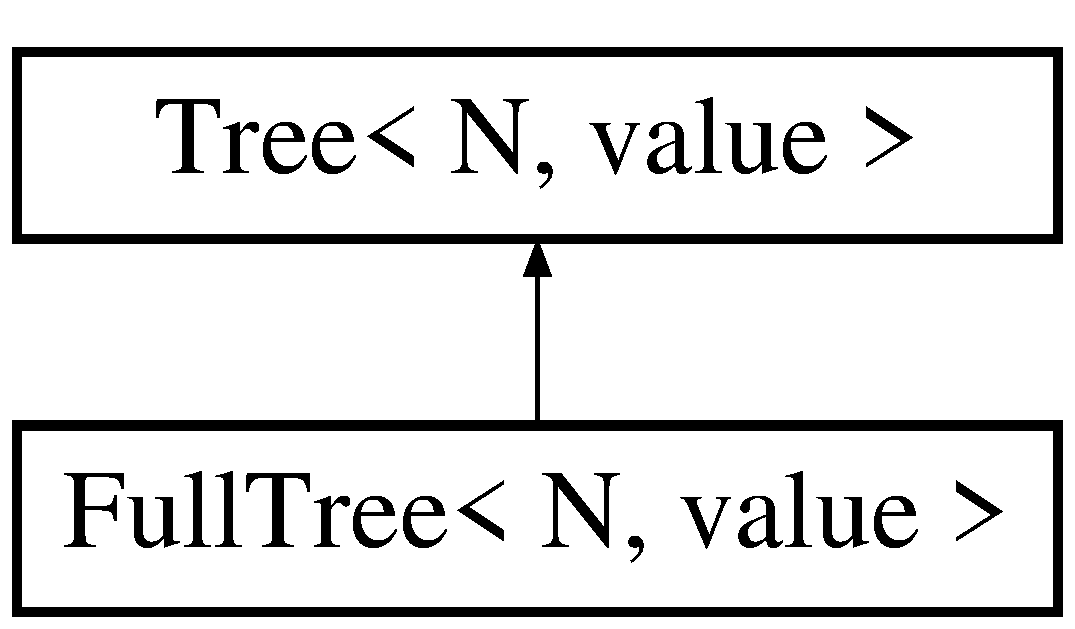
\includegraphics[height=2.000000cm]{classFullTree}
\end{center}
\end{figure}
\subsection*{Public Member Functions}
\begin{DoxyCompactItemize}
\item 
\mbox{\hyperlink{classFullTree_a7e91df045a1e04bb4d749d67300a1c3b}{Full\+Tree}} (\mbox{\hyperlink{definitions_8h_aedc0ad84d1e764530814f57ad931d02a}{real}} $\ast$length, \mbox{\hyperlink{definitions_8h_aedc0ad84d1e764530814f57ad931d02a}{real}} $\ast$coords)
\item 
void \mbox{\hyperlink{classFullTree_a1f880ec827fcd885759f6eafc76048be}{set\+Level}} (const \mbox{\hyperlink{definitions_8h_a69aa29b598b851b0640aa225a9e5d61d}{uint}} \&l)
\item 
void \mbox{\hyperlink{classFullTree_a2aadfbda309e246642550044712f98a0}{level}} (\mbox{\hyperlink{definitions_8h_af8682350bd8bb38ee9023f7a0a310add}{morton}}$<$ N $>$ key, \mbox{\hyperlink{definitions_8h_a69aa29b598b851b0640aa225a9e5d61d}{uint}} $\ast$level)
\item 
void \mbox{\hyperlink{classFullTree_abce6ea3ea3393373f32a5b7ccfcac976}{insert\+Key}} (\mbox{\hyperlink{definitions_8h_af8682350bd8bb38ee9023f7a0a310add}{morton}}$<$ N $>$ key)
\item 
\mbox{\hyperlink{definitions_8h_a69aa29b598b851b0640aa225a9e5d61d}{uint}} \mbox{\hyperlink{classFullTree_abed32a809a754eab0ae47257da1863b4}{get\+Level}} ()
\item 
void \mbox{\hyperlink{classFullTree_ade3b60e3f3622a49edb5b7a88e348667}{nbrs\+Constrcut}} (vector$<$ \mbox{\hyperlink{definitions_8h_a69aa29b598b851b0640aa225a9e5d61d}{uint}} $>$ \&Nbrs, \mbox{\hyperlink{definitions_8h_a69aa29b598b851b0640aa225a9e5d61d}{uint}} myrank)
\item 
bool \mbox{\hyperlink{classFullTree_acb1eec16a6b73e2a465b7a32319fe4f6}{is\+Boundary}} (\mbox{\hyperlink{definitions_8h_a69aa29b598b851b0640aa225a9e5d61d}{uint}} \&direction, \mbox{\hyperlink{definitions_8h_a69aa29b598b851b0640aa225a9e5d61d}{uint}} myrank)
\item 
\mbox{\hyperlink{definitions_8h_acf2396ef4de9eb8a6324b9f1a624ea85}{bitmap}}$<$ N, value $>$\+::iterator \mbox{\hyperlink{classFullTree_ad0432afb277be83e79d33e1a748648a3}{find}} (\mbox{\hyperlink{definitions_8h_af8682350bd8bb38ee9023f7a0a310add}{morton}}$<$ N $>$ key)
\item 
\mbox{\hyperlink{definitions_8h_a69aa29b598b851b0640aa225a9e5d61d}{uint}} \mbox{\hyperlink{classFullTree_a13bb6b68dea0e36255dbd7b057110806}{size}} ()
\item 
void \mbox{\hyperlink{classFullTree_a1b0a9b6f0f5155dd8847905ee8aa1b56}{convert\+Coord\+To\+Morton}} (\mbox{\hyperlink{definitions_8h_aedc0ad84d1e764530814f57ad931d02a}{real}} $\ast$xyz, \mbox{\hyperlink{definitions_8h_af8682350bd8bb38ee9023f7a0a310add}{morton}}$<$ N $>$ \&key)
\item 
void \mbox{\hyperlink{classFullTree_a71034640d78c83c761cc005a77f83afa}{assign\+Procs}} (vector$<$ \mbox{\hyperlink{definitions_8h_a69aa29b598b851b0640aa225a9e5d61d}{uint}} $>$ \&Nbrs, \mbox{\hyperlink{definitions_8h_a69aa29b598b851b0640aa225a9e5d61d}{uint}} myrank)
\item 
void \mbox{\hyperlink{classFullTree_ae820d50b6b006f8bcdbcbcc5aa2fc9f6}{find\+Flip\+Level}} (\mbox{\hyperlink{definitions_8h_af8682350bd8bb38ee9023f7a0a310add}{morton}}$<$ \mbox{\hyperlink{params_8h_a869e77c8856c40dc7369197ee4ee8059ab8317ae7816b83628f4e2bcff586e2f5}{W\+S\+I\+ZE}} $>$ key, \mbox{\hyperlink{definitions_8h_a69aa29b598b851b0640aa225a9e5d61d}{uint}} \mbox{\hyperlink{classFullTree_a1bcc4d0daf8ad12569054422379b556f}{fixedlevel}}, \mbox{\hyperlink{definitions_8h_a69aa29b598b851b0640aa225a9e5d61d}{uint}} $\ast$changedirectionlevel, \mbox{\hyperlink{definitions_8h_a69aa29b598b851b0640aa225a9e5d61d}{uint}} $\ast$direction)
\item 
void \mbox{\hyperlink{classFullTree_ad3d930eda377be811df22070f6364865}{flip\+For\+Nbr}} (\mbox{\hyperlink{definitions_8h_af8682350bd8bb38ee9023f7a0a310add}{morton}}$<$ \mbox{\hyperlink{params_8h_a869e77c8856c40dc7369197ee4ee8059ab8317ae7816b83628f4e2bcff586e2f5}{W\+S\+I\+ZE}} $>$ $\ast$key, \mbox{\hyperlink{definitions_8h_a69aa29b598b851b0640aa225a9e5d61d}{uint}} \mbox{\hyperlink{classFullTree_a1bcc4d0daf8ad12569054422379b556f}{fixedlevel}}, \mbox{\hyperlink{definitions_8h_a69aa29b598b851b0640aa225a9e5d61d}{uint}} $\ast$changedirectionlevel, \mbox{\hyperlink{definitions_8h_a69aa29b598b851b0640aa225a9e5d61d}{uint}} $\ast$direction)
\item 
\mbox{\hyperlink{definitions_8h_acf2396ef4de9eb8a6324b9f1a624ea85}{bitmap}}$<$ N, value $>$\+::iterator \mbox{\hyperlink{classFullTree_af2fbecbd352a329634a6fdc35f519968}{begin}} ()
\item 
\mbox{\hyperlink{definitions_8h_acf2396ef4de9eb8a6324b9f1a624ea85}{bitmap}}$<$ N, value $>$\+::iterator \mbox{\hyperlink{classFullTree_a692131b057639fecdb1934b734cff1bb}{end}} ()
\item 
\mbox{\hyperlink{classFullTree_a8b2e043f141edee101d55ad0ea497d9f}{$\sim$\+Full\+Tree}} ()
\end{DoxyCompactItemize}
\subsection*{Private Attributes}
\begin{DoxyCompactItemize}
\item 
\mbox{\hyperlink{definitions_8h_a69aa29b598b851b0640aa225a9e5d61d}{uint}} \mbox{\hyperlink{classFullTree_a1bcc4d0daf8ad12569054422379b556f}{fixedlevel}}
\item 
\mbox{\hyperlink{definitions_8h_acf2396ef4de9eb8a6324b9f1a624ea85}{bitmap}}$<$ N, value $>$ \mbox{\hyperlink{classFullTree_a98c8b05985b0cf911db0d6252aa98396}{mesh}}
\item 
std\+::unordered\+\_\+map$<$ \mbox{\hyperlink{definitions_8h_af8682350bd8bb38ee9023f7a0a310add}{morton}}$<$ N $>$, int $>$ \mbox{\hyperlink{classFullTree_aa4cfcbc1c6029ecd353759159a8d8844}{refinelist}}
\item 
\mbox{\hyperlink{definitions_8h_a55821d7929f3f16aaf1466129c209492}{bitvector}}$<$ N $>$ \mbox{\hyperlink{classFullTree_a91af9d7a974af6484dc61c20cd78d1bc}{morton\+S\+TL}}
\item 
std\+::unordered\+\_\+map$<$ \mbox{\hyperlink{definitions_8h_af8682350bd8bb38ee9023f7a0a310add}{morton}}$<$ N $>$, int $>$ \mbox{\hyperlink{classFullTree_a4c87e86cce1c7f0f92651ad87d3823ec}{derefinelist}}
\end{DoxyCompactItemize}
\subsection*{Additional Inherited Members}


\subsection{Detailed Description}
\subsubsection*{template$<$size\+\_\+t N, typename value$>$\newline
class Full\+Tree$<$ N, value $>$}

This Class is specifically designed for weak analysis to operate on the fulltree topology in this class, level is preset by the user and the level function is redefined to make use of the polymorphism. 

\subsection{Constructor \& Destructor Documentation}
\mbox{\Hypertarget{classFullTree_a7e91df045a1e04bb4d749d67300a1c3b}\label{classFullTree_a7e91df045a1e04bb4d749d67300a1c3b}} 
\index{Full\+Tree@{Full\+Tree}!Full\+Tree@{Full\+Tree}}
\index{Full\+Tree@{Full\+Tree}!Full\+Tree@{Full\+Tree}}
\subsubsection{\texorpdfstring{Full\+Tree()}{FullTree()}}
{\footnotesize\ttfamily template$<$size\+\_\+t N, typename value$>$ \\
\mbox{\hyperlink{classFullTree}{Full\+Tree}}$<$ N, value $>$\+::\mbox{\hyperlink{classFullTree}{Full\+Tree}} (\begin{DoxyParamCaption}\item[{\mbox{\hyperlink{definitions_8h_aedc0ad84d1e764530814f57ad931d02a}{real}} $\ast$}]{length,  }\item[{\mbox{\hyperlink{definitions_8h_aedc0ad84d1e764530814f57ad931d02a}{real}} $\ast$}]{coords }\end{DoxyParamCaption})\hspace{0.3cm}{\ttfamily [inline]}}

\mbox{\Hypertarget{classFullTree_a8b2e043f141edee101d55ad0ea497d9f}\label{classFullTree_a8b2e043f141edee101d55ad0ea497d9f}} 
\index{Full\+Tree@{Full\+Tree}!````~Full\+Tree@{$\sim$\+Full\+Tree}}
\index{````~Full\+Tree@{$\sim$\+Full\+Tree}!Full\+Tree@{Full\+Tree}}
\subsubsection{\texorpdfstring{$\sim$\+Full\+Tree()}{~FullTree()}}
{\footnotesize\ttfamily template$<$size\+\_\+t N, typename value$>$ \\
\mbox{\hyperlink{classFullTree}{Full\+Tree}}$<$ N, value $>$\+::$\sim$\mbox{\hyperlink{classFullTree}{Full\+Tree}} (\begin{DoxyParamCaption}{ }\end{DoxyParamCaption})\hspace{0.3cm}{\ttfamily [inline]}}



\subsection{Member Function Documentation}
\mbox{\Hypertarget{classFullTree_a71034640d78c83c761cc005a77f83afa}\label{classFullTree_a71034640d78c83c761cc005a77f83afa}} 
\index{Full\+Tree@{Full\+Tree}!assign\+Procs@{assign\+Procs}}
\index{assign\+Procs@{assign\+Procs}!Full\+Tree@{Full\+Tree}}
\subsubsection{\texorpdfstring{assign\+Procs()}{assignProcs()}}
{\footnotesize\ttfamily template$<$size\+\_\+t N, typename value $>$ \\
void \mbox{\hyperlink{classFullTree}{Full\+Tree}}$<$ N, value $>$\+::assign\+Procs (\begin{DoxyParamCaption}\item[{vector$<$ \mbox{\hyperlink{definitions_8h_a69aa29b598b851b0640aa225a9e5d61d}{uint}} $>$ \&}]{Nbrs,  }\item[{\mbox{\hyperlink{definitions_8h_a69aa29b598b851b0640aa225a9e5d61d}{uint}}}]{myrank }\end{DoxyParamCaption})}

\mbox{\Hypertarget{classFullTree_af2fbecbd352a329634a6fdc35f519968}\label{classFullTree_af2fbecbd352a329634a6fdc35f519968}} 
\index{Full\+Tree@{Full\+Tree}!begin@{begin}}
\index{begin@{begin}!Full\+Tree@{Full\+Tree}}
\subsubsection{\texorpdfstring{begin()}{begin()}}
{\footnotesize\ttfamily template$<$size\+\_\+t N, typename value $>$ \\
\mbox{\hyperlink{definitions_8h_acf2396ef4de9eb8a6324b9f1a624ea85}{bitmap}}$<$ N, value $>$\+::iterator \mbox{\hyperlink{classFullTree}{Full\+Tree}}$<$ N, value $>$\+::begin (\begin{DoxyParamCaption}{ }\end{DoxyParamCaption})\hspace{0.3cm}{\ttfamily [virtual]}}

iterator returning the first object 

Reimplemented from \mbox{\hyperlink{classTree_aa9a32f0e006ee027c037669b8b1c7d01}{Tree$<$ N, value $>$}}.

\mbox{\Hypertarget{classFullTree_a1b0a9b6f0f5155dd8847905ee8aa1b56}\label{classFullTree_a1b0a9b6f0f5155dd8847905ee8aa1b56}} 
\index{Full\+Tree@{Full\+Tree}!convert\+Coord\+To\+Morton@{convert\+Coord\+To\+Morton}}
\index{convert\+Coord\+To\+Morton@{convert\+Coord\+To\+Morton}!Full\+Tree@{Full\+Tree}}
\subsubsection{\texorpdfstring{convert\+Coord\+To\+Morton()}{convertCoordToMorton()}}
{\footnotesize\ttfamily template$<$size\+\_\+t N, typename value $>$ \\
void \mbox{\hyperlink{classFullTree}{Full\+Tree}}$<$ N, value $>$\+::convert\+Coord\+To\+Morton (\begin{DoxyParamCaption}\item[{\mbox{\hyperlink{definitions_8h_aedc0ad84d1e764530814f57ad931d02a}{real}} $\ast$}]{xyz,  }\item[{\mbox{\hyperlink{definitions_8h_af8682350bd8bb38ee9023f7a0a310add}{morton}}$<$ N $>$ \&}]{key }\end{DoxyParamCaption})\hspace{0.3cm}{\ttfamily [virtual]}}

!$<$ this function is to find a value given the key 

Reimplemented from \mbox{\hyperlink{classTree_a945d137d27bb55d9feb5762ac821572a}{Tree$<$ N, value $>$}}.

\mbox{\Hypertarget{classFullTree_a692131b057639fecdb1934b734cff1bb}\label{classFullTree_a692131b057639fecdb1934b734cff1bb}} 
\index{Full\+Tree@{Full\+Tree}!end@{end}}
\index{end@{end}!Full\+Tree@{Full\+Tree}}
\subsubsection{\texorpdfstring{end()}{end()}}
{\footnotesize\ttfamily template$<$size\+\_\+t N, typename value $>$ \\
\mbox{\hyperlink{definitions_8h_acf2396ef4de9eb8a6324b9f1a624ea85}{bitmap}}$<$ N, value $>$\+::iterator \mbox{\hyperlink{classFullTree}{Full\+Tree}}$<$ N, value $>$\+::end (\begin{DoxyParamCaption}{ }\end{DoxyParamCaption})\hspace{0.3cm}{\ttfamily [virtual]}}

iterator returning the last object 

Reimplemented from \mbox{\hyperlink{classTree_a780c144c3fa4f648e7c616d7010721b0}{Tree$<$ N, value $>$}}.

\mbox{\Hypertarget{classFullTree_ad0432afb277be83e79d33e1a748648a3}\label{classFullTree_ad0432afb277be83e79d33e1a748648a3}} 
\index{Full\+Tree@{Full\+Tree}!find@{find}}
\index{find@{find}!Full\+Tree@{Full\+Tree}}
\subsubsection{\texorpdfstring{find()}{find()}}
{\footnotesize\ttfamily template$<$size\+\_\+t N, typename value $>$ \\
\mbox{\hyperlink{definitions_8h_acf2396ef4de9eb8a6324b9f1a624ea85}{bitmap}}$<$ N, value $>$\+::iterator \mbox{\hyperlink{classFullTree}{Full\+Tree}}$<$ N, value $>$\+::find (\begin{DoxyParamCaption}\item[{\mbox{\hyperlink{definitions_8h_af8682350bd8bb38ee9023f7a0a310add}{morton}}$<$ N $>$}]{key }\end{DoxyParamCaption})\hspace{0.3cm}{\ttfamily [virtual]}}

this function is to find a value given the key

!$<$ this function is to find a value given the key 

Reimplemented from \mbox{\hyperlink{classTree_a8337d6639f90ef96e4d42e1cbfab61dd}{Tree$<$ N, value $>$}}.

\mbox{\Hypertarget{classFullTree_ae820d50b6b006f8bcdbcbcc5aa2fc9f6}\label{classFullTree_ae820d50b6b006f8bcdbcbcc5aa2fc9f6}} 
\index{Full\+Tree@{Full\+Tree}!find\+Flip\+Level@{find\+Flip\+Level}}
\index{find\+Flip\+Level@{find\+Flip\+Level}!Full\+Tree@{Full\+Tree}}
\subsubsection{\texorpdfstring{find\+Flip\+Level()}{findFlipLevel()}}
{\footnotesize\ttfamily template$<$size\+\_\+t N, typename value $>$ \\
void \mbox{\hyperlink{classFullTree}{Full\+Tree}}$<$ N, value $>$\+::find\+Flip\+Level (\begin{DoxyParamCaption}\item[{\mbox{\hyperlink{definitions_8h_af8682350bd8bb38ee9023f7a0a310add}{morton}}$<$ \mbox{\hyperlink{params_8h_a869e77c8856c40dc7369197ee4ee8059ab8317ae7816b83628f4e2bcff586e2f5}{W\+S\+I\+ZE}} $>$}]{key,  }\item[{\mbox{\hyperlink{definitions_8h_a69aa29b598b851b0640aa225a9e5d61d}{uint}}}]{fixedlevel,  }\item[{\mbox{\hyperlink{definitions_8h_a69aa29b598b851b0640aa225a9e5d61d}{uint}} $\ast$}]{changedirectionlevel,  }\item[{\mbox{\hyperlink{definitions_8h_a69aa29b598b851b0640aa225a9e5d61d}{uint}} $\ast$}]{direction }\end{DoxyParamCaption})}

\mbox{\Hypertarget{classFullTree_ad3d930eda377be811df22070f6364865}\label{classFullTree_ad3d930eda377be811df22070f6364865}} 
\index{Full\+Tree@{Full\+Tree}!flip\+For\+Nbr@{flip\+For\+Nbr}}
\index{flip\+For\+Nbr@{flip\+For\+Nbr}!Full\+Tree@{Full\+Tree}}
\subsubsection{\texorpdfstring{flip\+For\+Nbr()}{flipForNbr()}}
{\footnotesize\ttfamily template$<$size\+\_\+t N, typename value $>$ \\
void \mbox{\hyperlink{classFullTree}{Full\+Tree}}$<$ N, value $>$\+::flip\+For\+Nbr (\begin{DoxyParamCaption}\item[{\mbox{\hyperlink{definitions_8h_af8682350bd8bb38ee9023f7a0a310add}{morton}}$<$ \mbox{\hyperlink{params_8h_a869e77c8856c40dc7369197ee4ee8059ab8317ae7816b83628f4e2bcff586e2f5}{W\+S\+I\+ZE}} $>$ $\ast$}]{key,  }\item[{\mbox{\hyperlink{definitions_8h_a69aa29b598b851b0640aa225a9e5d61d}{uint}}}]{fixedlevel,  }\item[{\mbox{\hyperlink{definitions_8h_a69aa29b598b851b0640aa225a9e5d61d}{uint}} $\ast$}]{changedirectionlevel,  }\item[{\mbox{\hyperlink{definitions_8h_a69aa29b598b851b0640aa225a9e5d61d}{uint}} $\ast$}]{direction }\end{DoxyParamCaption})}

\mbox{\Hypertarget{classFullTree_abed32a809a754eab0ae47257da1863b4}\label{classFullTree_abed32a809a754eab0ae47257da1863b4}} 
\index{Full\+Tree@{Full\+Tree}!get\+Level@{get\+Level}}
\index{get\+Level@{get\+Level}!Full\+Tree@{Full\+Tree}}
\subsubsection{\texorpdfstring{get\+Level()}{getLevel()}}
{\footnotesize\ttfamily template$<$size\+\_\+t N, typename value $>$ \\
\mbox{\hyperlink{definitions_8h_a69aa29b598b851b0640aa225a9e5d61d}{uint}} \mbox{\hyperlink{classFullTree}{Full\+Tree}}$<$ N, value $>$\+::get\+Level (\begin{DoxyParamCaption}{ }\end{DoxyParamCaption})}

\mbox{\Hypertarget{classFullTree_abce6ea3ea3393373f32a5b7ccfcac976}\label{classFullTree_abce6ea3ea3393373f32a5b7ccfcac976}} 
\index{Full\+Tree@{Full\+Tree}!insert\+Key@{insert\+Key}}
\index{insert\+Key@{insert\+Key}!Full\+Tree@{Full\+Tree}}
\subsubsection{\texorpdfstring{insert\+Key()}{insertKey()}}
{\footnotesize\ttfamily template$<$size\+\_\+t N, typename value $>$ \\
void \mbox{\hyperlink{classFullTree}{Full\+Tree}}$<$ N, value $>$\+::insert\+Key (\begin{DoxyParamCaption}\item[{\mbox{\hyperlink{definitions_8h_af8682350bd8bb38ee9023f7a0a310add}{morton}}$<$ N $>$}]{key }\end{DoxyParamCaption})}

\mbox{\Hypertarget{classFullTree_acb1eec16a6b73e2a465b7a32319fe4f6}\label{classFullTree_acb1eec16a6b73e2a465b7a32319fe4f6}} 
\index{Full\+Tree@{Full\+Tree}!is\+Boundary@{is\+Boundary}}
\index{is\+Boundary@{is\+Boundary}!Full\+Tree@{Full\+Tree}}
\subsubsection{\texorpdfstring{is\+Boundary()}{isBoundary()}}
{\footnotesize\ttfamily template$<$size\+\_\+t N, typename value $>$ \\
bool \mbox{\hyperlink{classFullTree}{Full\+Tree}}$<$ N, value $>$\+::is\+Boundary (\begin{DoxyParamCaption}\item[{\mbox{\hyperlink{definitions_8h_a69aa29b598b851b0640aa225a9e5d61d}{uint}} \&}]{direction,  }\item[{\mbox{\hyperlink{definitions_8h_a69aa29b598b851b0640aa225a9e5d61d}{uint}}}]{myrank }\end{DoxyParamCaption})}

\mbox{\Hypertarget{classFullTree_a2aadfbda309e246642550044712f98a0}\label{classFullTree_a2aadfbda309e246642550044712f98a0}} 
\index{Full\+Tree@{Full\+Tree}!level@{level}}
\index{level@{level}!Full\+Tree@{Full\+Tree}}
\subsubsection{\texorpdfstring{level()}{level()}}
{\footnotesize\ttfamily template$<$size\+\_\+t N, typename value $>$ \\
void \mbox{\hyperlink{classFullTree}{Full\+Tree}}$<$ N, value $>$\+::level (\begin{DoxyParamCaption}\item[{\mbox{\hyperlink{definitions_8h_af8682350bd8bb38ee9023f7a0a310add}{morton}}$<$ N $>$}]{key,  }\item[{\mbox{\hyperlink{definitions_8h_a69aa29b598b851b0640aa225a9e5d61d}{uint}} $\ast$}]{level }\end{DoxyParamCaption})\hspace{0.3cm}{\ttfamily [virtual]}}

obtains the level of the element from morton key to prevent unnecesary bit operation, the morton code is placed from starting from left hand side

now look and see if any siblings exist 

Reimplemented from \mbox{\hyperlink{classTree_a01f065cafedac5e2845e9d17bf87b783}{Tree$<$ N, value $>$}}.

\mbox{\Hypertarget{classFullTree_ade3b60e3f3622a49edb5b7a88e348667}\label{classFullTree_ade3b60e3f3622a49edb5b7a88e348667}} 
\index{Full\+Tree@{Full\+Tree}!nbrs\+Constrcut@{nbrs\+Constrcut}}
\index{nbrs\+Constrcut@{nbrs\+Constrcut}!Full\+Tree@{Full\+Tree}}
\subsubsection{\texorpdfstring{nbrs\+Constrcut()}{nbrsConstrcut()}}
{\footnotesize\ttfamily template$<$size\+\_\+t N, typename value $>$ \\
void \mbox{\hyperlink{classFullTree}{Full\+Tree}}$<$ N, value $>$\+::nbrs\+Constrcut (\begin{DoxyParamCaption}\item[{vector$<$ \mbox{\hyperlink{definitions_8h_a69aa29b598b851b0640aa225a9e5d61d}{uint}} $>$ \&}]{Nbrs,  }\item[{\mbox{\hyperlink{definitions_8h_a69aa29b598b851b0640aa225a9e5d61d}{uint}}}]{myrank }\end{DoxyParamCaption})}

\mbox{\Hypertarget{classFullTree_a1f880ec827fcd885759f6eafc76048be}\label{classFullTree_a1f880ec827fcd885759f6eafc76048be}} 
\index{Full\+Tree@{Full\+Tree}!set\+Level@{set\+Level}}
\index{set\+Level@{set\+Level}!Full\+Tree@{Full\+Tree}}
\subsubsection{\texorpdfstring{set\+Level()}{setLevel()}}
{\footnotesize\ttfamily template$<$size\+\_\+t N, typename value $>$ \\
void \mbox{\hyperlink{classFullTree}{Full\+Tree}}$<$ N, value $>$\+::set\+Level (\begin{DoxyParamCaption}\item[{const \mbox{\hyperlink{definitions_8h_a69aa29b598b851b0640aa225a9e5d61d}{uint}} \&}]{l }\end{DoxyParamCaption})}

constructor sets the maximum level for refinement \mbox{\Hypertarget{classFullTree_a13bb6b68dea0e36255dbd7b057110806}\label{classFullTree_a13bb6b68dea0e36255dbd7b057110806}} 
\index{Full\+Tree@{Full\+Tree}!size@{size}}
\index{size@{size}!Full\+Tree@{Full\+Tree}}
\subsubsection{\texorpdfstring{size()}{size()}}
{\footnotesize\ttfamily template$<$size\+\_\+t N, typename value $>$ \\
\mbox{\hyperlink{definitions_8h_a69aa29b598b851b0640aa225a9e5d61d}{uint}} \mbox{\hyperlink{classFullTree}{Full\+Tree}}$<$ N, value $>$\+::size (\begin{DoxyParamCaption}{ }\end{DoxyParamCaption})\hspace{0.3cm}{\ttfamily [virtual]}}

returns the size of the mesh 

Reimplemented from \mbox{\hyperlink{classTree_a8af31c93aa821f0d853e920bcba1829a}{Tree$<$ N, value $>$}}.



\subsection{Member Data Documentation}
\mbox{\Hypertarget{classFullTree_a4c87e86cce1c7f0f92651ad87d3823ec}\label{classFullTree_a4c87e86cce1c7f0f92651ad87d3823ec}} 
\index{Full\+Tree@{Full\+Tree}!derefinelist@{derefinelist}}
\index{derefinelist@{derefinelist}!Full\+Tree@{Full\+Tree}}
\subsubsection{\texorpdfstring{derefinelist}{derefinelist}}
{\footnotesize\ttfamily template$<$size\+\_\+t N, typename value$>$ \\
std\+::unordered\+\_\+map$<$\mbox{\hyperlink{definitions_8h_af8682350bd8bb38ee9023f7a0a310add}{morton}}$<$N$>$, int$>$ \mbox{\hyperlink{classFullTree}{Full\+Tree}}$<$ N, value $>$\+::derefinelist\hspace{0.3cm}{\ttfamily [private]}}

list of elements tagged to be removed, due to 4\+:1 balance this listi \mbox{\Hypertarget{classFullTree_a1bcc4d0daf8ad12569054422379b556f}\label{classFullTree_a1bcc4d0daf8ad12569054422379b556f}} 
\index{Full\+Tree@{Full\+Tree}!fixedlevel@{fixedlevel}}
\index{fixedlevel@{fixedlevel}!Full\+Tree@{Full\+Tree}}
\subsubsection{\texorpdfstring{fixedlevel}{fixedlevel}}
{\footnotesize\ttfamily template$<$size\+\_\+t N, typename value$>$ \\
\mbox{\hyperlink{definitions_8h_a69aa29b598b851b0640aa225a9e5d61d}{uint}} \mbox{\hyperlink{classFullTree}{Full\+Tree}}$<$ N, value $>$\+::fixedlevel\hspace{0.3cm}{\ttfamily [private]}}

maximum level of full tree \mbox{\Hypertarget{classFullTree_a98c8b05985b0cf911db0d6252aa98396}\label{classFullTree_a98c8b05985b0cf911db0d6252aa98396}} 
\index{Full\+Tree@{Full\+Tree}!mesh@{mesh}}
\index{mesh@{mesh}!Full\+Tree@{Full\+Tree}}
\subsubsection{\texorpdfstring{mesh}{mesh}}
{\footnotesize\ttfamily template$<$size\+\_\+t N, typename value$>$ \\
\mbox{\hyperlink{definitions_8h_acf2396ef4de9eb8a6324b9f1a624ea85}{bitmap}}$<$N, value$>$ \mbox{\hyperlink{classFullTree}{Full\+Tree}}$<$ N, value $>$\+::mesh\hspace{0.3cm}{\ttfamily [private]}}

\mbox{\Hypertarget{classFullTree_a91af9d7a974af6484dc61c20cd78d1bc}\label{classFullTree_a91af9d7a974af6484dc61c20cd78d1bc}} 
\index{Full\+Tree@{Full\+Tree}!morton\+S\+TL@{morton\+S\+TL}}
\index{morton\+S\+TL@{morton\+S\+TL}!Full\+Tree@{Full\+Tree}}
\subsubsection{\texorpdfstring{morton\+S\+TL}{mortonSTL}}
{\footnotesize\ttfamily template$<$size\+\_\+t N, typename value$>$ \\
\mbox{\hyperlink{definitions_8h_a55821d7929f3f16aaf1466129c209492}{bitvector}}$<$N$>$ \mbox{\hyperlink{classFullTree}{Full\+Tree}}$<$ N, value $>$\+::morton\+S\+TL\hspace{0.3cm}{\ttfamily [private]}}

vector to store geometric points in morton code \mbox{\Hypertarget{classFullTree_aa4cfcbc1c6029ecd353759159a8d8844}\label{classFullTree_aa4cfcbc1c6029ecd353759159a8d8844}} 
\index{Full\+Tree@{Full\+Tree}!refinelist@{refinelist}}
\index{refinelist@{refinelist}!Full\+Tree@{Full\+Tree}}
\subsubsection{\texorpdfstring{refinelist}{refinelist}}
{\footnotesize\ttfamily template$<$size\+\_\+t N, typename value$>$ \\
std\+::unordered\+\_\+map$<$\mbox{\hyperlink{definitions_8h_af8682350bd8bb38ee9023f7a0a310add}{morton}}$<$N$>$, int$>$ \mbox{\hyperlink{classFullTree}{Full\+Tree}}$<$ N, value $>$\+::refinelist\hspace{0.3cm}{\ttfamily [private]}}

list of elements tagged to be refined 

The documentation for this class was generated from the following files\+:\begin{DoxyCompactItemize}
\item 
/ihome/isenocak/jaber/\+Morton\+\_\+\+Parallel\+\_\+v0/test/\+Morton\+\_\+\+Parallel\+\_\+v0/src/include/\mbox{\hyperlink{tree_8h}{tree.\+h}}\item 
/ihome/isenocak/jaber/\+Morton\+\_\+\+Parallel\+\_\+v0/test/\+Morton\+\_\+\+Parallel\+\_\+v0/src/\mbox{\hyperlink{full__tree_8cpp}{full\+\_\+tree.\+cpp}}\end{DoxyCompactItemize}

\hypertarget{classGeomSTL}{}\section{Geom\+S\+TL Class Reference}
\label{classGeomSTL}\index{Geom\+S\+TL@{Geom\+S\+TL}}


{\ttfamily \#include $<$geom\+S\+T\+L.\+h$>$}

\subsection*{Public Member Functions}
\begin{DoxyCompactItemize}
\item 
\mbox{\hyperlink{classGeomSTL_a90b2b4613d18ae27f53393233b063207}{Geom\+S\+TL}} ()
\item 
void \mbox{\hyperlink{classGeomSTL_abda226b5dab2871a7b61bfaf2203234d}{construct}} (\mbox{\hyperlink{definitions_8h_aedc0ad84d1e764530814f57ad931d02a}{real}} $\ast$xyz1)
\item 
\mbox{\hyperlink{structstl__data}{stl\+\_\+data}} \mbox{\hyperlink{classGeomSTL_ab73af5ba40ffa45cbff467fc6421088c}{parse\+\_\+stl}} (const std\+::string \&stl\+\_\+path)
\item 
float \mbox{\hyperlink{classGeomSTL_a4da4da9fdbd99722ca7e2005420a8e68}{parse\+\_\+float}} (std\+::ifstream \&s)
\item 
\mbox{\hyperlink{structpoint}{point}} \mbox{\hyperlink{classGeomSTL_a188d94b64201e5d2ee6ce8919742c240}{parse\+\_\+point}} (std\+::ifstream \&s)
\item 
\mbox{\hyperlink{structstl__data}{stl\+\_\+data}} \mbox{\hyperlink{classGeomSTL_a4dd58852b67375603db2735f4ab119ce}{parse\+S\+TL}} (const std\+::string \&stl\+\_\+path)
\item 
void \mbox{\hyperlink{classGeomSTL_aeccef8dc47681bd8b594bdcf93fdf910}{read\+S\+T\+L\+Geom}} (char $\ast$argv\mbox{[}$\,$\mbox{]}, const \mbox{\hyperlink{definitions_8h_aedc0ad84d1e764530814f57ad931d02a}{real}} $\ast$\mbox{\hyperlink{classGeomSTL_a38716d8c3db44ebc059e020d2ce926b2}{xyz}})
\item 
void \mbox{\hyperlink{classGeomSTL_a55768801abe34a2326c1a5013924faac}{check\+Mesh}} (std\+::vector$<$ \mbox{\hyperlink{structtriangle}{triangle}} $>$ \&triangles)
\end{DoxyCompactItemize}
\subsection*{Private Attributes}
\begin{DoxyCompactItemize}
\item 
int \mbox{\hyperlink{classGeomSTL_ae5999187224ca4a905f6281f83ad10d4}{geom\+\_\+nn}}
\item 
\mbox{\hyperlink{definitions_8h_aedc0ad84d1e764530814f57ad931d02a}{real}} $\ast$ \mbox{\hyperlink{classGeomSTL_aa042c614009a5473c8bd34bf6cda0561}{geom\+\_\+xyz}}
\item 
\mbox{\hyperlink{definitions_8h_aedc0ad84d1e764530814f57ad931d02a}{real}} $\ast$\+\_\+\+\_\+restrict\+\_\+\+\_\+ \mbox{\hyperlink{classGeomSTL_a090ec3d4d4a5be7eb0a0874ce91b07a3}{triangle\+\_\+center}}
\item 
\mbox{\hyperlink{definitions_8h_aedc0ad84d1e764530814f57ad931d02a}{real}} \mbox{\hyperlink{classGeomSTL_a38716d8c3db44ebc059e020d2ce926b2}{xyz}} \mbox{[}6\mbox{]}
\end{DoxyCompactItemize}
\subsection*{Friends}
\begin{DoxyCompactItemize}
\item 
{\footnotesize template$<$size\+\_\+t N, typename Nvalue , size\+\_\+t M, typename Mvalue $>$ }\\class \mbox{\hyperlink{classGeomSTL_a8d90a8b4dd53f0733e15d6eed6d2dcdd}{Rebl\+Amr}}
\end{DoxyCompactItemize}


\subsection{Constructor \& Destructor Documentation}
\mbox{\Hypertarget{classGeomSTL_a90b2b4613d18ae27f53393233b063207}\label{classGeomSTL_a90b2b4613d18ae27f53393233b063207}} 
\index{Geom\+S\+TL@{Geom\+S\+TL}!Geom\+S\+TL@{Geom\+S\+TL}}
\index{Geom\+S\+TL@{Geom\+S\+TL}!Geom\+S\+TL@{Geom\+S\+TL}}
\subsubsection{\texorpdfstring{Geom\+S\+T\+L()}{GeomSTL()}}
{\footnotesize\ttfamily Geom\+S\+T\+L\+::\+Geom\+S\+TL (\begin{DoxyParamCaption}{ }\end{DoxyParamCaption})\hspace{0.3cm}{\ttfamily [inline]}}



\subsection{Member Function Documentation}
\mbox{\Hypertarget{classGeomSTL_a55768801abe34a2326c1a5013924faac}\label{classGeomSTL_a55768801abe34a2326c1a5013924faac}} 
\index{Geom\+S\+TL@{Geom\+S\+TL}!check\+Mesh@{check\+Mesh}}
\index{check\+Mesh@{check\+Mesh}!Geom\+S\+TL@{Geom\+S\+TL}}
\subsubsection{\texorpdfstring{check\+Mesh()}{checkMesh()}}
{\footnotesize\ttfamily void Geom\+S\+T\+L\+::check\+Mesh (\begin{DoxyParamCaption}\item[{std\+::vector$<$ \mbox{\hyperlink{structtriangle}{triangle}} $>$ \&}]{triangles }\end{DoxyParamCaption})}

\mbox{\Hypertarget{classGeomSTL_abda226b5dab2871a7b61bfaf2203234d}\label{classGeomSTL_abda226b5dab2871a7b61bfaf2203234d}} 
\index{Geom\+S\+TL@{Geom\+S\+TL}!construct@{construct}}
\index{construct@{construct}!Geom\+S\+TL@{Geom\+S\+TL}}
\subsubsection{\texorpdfstring{construct()}{construct()}}
{\footnotesize\ttfamily void Geom\+S\+T\+L\+::construct (\begin{DoxyParamCaption}\item[{\mbox{\hyperlink{definitions_8h_aedc0ad84d1e764530814f57ad931d02a}{real}} $\ast$}]{xyz1 }\end{DoxyParamCaption})}

\mbox{\Hypertarget{classGeomSTL_a4da4da9fdbd99722ca7e2005420a8e68}\label{classGeomSTL_a4da4da9fdbd99722ca7e2005420a8e68}} 
\index{Geom\+S\+TL@{Geom\+S\+TL}!parse\+\_\+float@{parse\+\_\+float}}
\index{parse\+\_\+float@{parse\+\_\+float}!Geom\+S\+TL@{Geom\+S\+TL}}
\subsubsection{\texorpdfstring{parse\+\_\+float()}{parse\_float()}}
{\footnotesize\ttfamily float Geom\+S\+T\+L\+::parse\+\_\+float (\begin{DoxyParamCaption}\item[{std\+::ifstream \&}]{s }\end{DoxyParamCaption})}

\mbox{\Hypertarget{classGeomSTL_a188d94b64201e5d2ee6ce8919742c240}\label{classGeomSTL_a188d94b64201e5d2ee6ce8919742c240}} 
\index{Geom\+S\+TL@{Geom\+S\+TL}!parse\+\_\+point@{parse\+\_\+point}}
\index{parse\+\_\+point@{parse\+\_\+point}!Geom\+S\+TL@{Geom\+S\+TL}}
\subsubsection{\texorpdfstring{parse\+\_\+point()}{parse\_point()}}
{\footnotesize\ttfamily \mbox{\hyperlink{structpoint}{point}} Geom\+S\+T\+L\+::parse\+\_\+point (\begin{DoxyParamCaption}\item[{std\+::ifstream \&}]{s }\end{DoxyParamCaption})}

\mbox{\Hypertarget{classGeomSTL_ab73af5ba40ffa45cbff467fc6421088c}\label{classGeomSTL_ab73af5ba40ffa45cbff467fc6421088c}} 
\index{Geom\+S\+TL@{Geom\+S\+TL}!parse\+\_\+stl@{parse\+\_\+stl}}
\index{parse\+\_\+stl@{parse\+\_\+stl}!Geom\+S\+TL@{Geom\+S\+TL}}
\subsubsection{\texorpdfstring{parse\+\_\+stl()}{parse\_stl()}}
{\footnotesize\ttfamily \mbox{\hyperlink{structstl__data}{stl\+\_\+data}} Geom\+S\+T\+L\+::parse\+\_\+stl (\begin{DoxyParamCaption}\item[{const std\+::string \&}]{stl\+\_\+path }\end{DoxyParamCaption})}

\mbox{\Hypertarget{classGeomSTL_a4dd58852b67375603db2735f4ab119ce}\label{classGeomSTL_a4dd58852b67375603db2735f4ab119ce}} 
\index{Geom\+S\+TL@{Geom\+S\+TL}!parse\+S\+TL@{parse\+S\+TL}}
\index{parse\+S\+TL@{parse\+S\+TL}!Geom\+S\+TL@{Geom\+S\+TL}}
\subsubsection{\texorpdfstring{parse\+S\+T\+L()}{parseSTL()}}
{\footnotesize\ttfamily \mbox{\hyperlink{structstl__data}{stl\+\_\+data}} Geom\+S\+T\+L\+::parse\+S\+TL (\begin{DoxyParamCaption}\item[{const std\+::string \&}]{stl\+\_\+path }\end{DoxyParamCaption})}

\mbox{\Hypertarget{classGeomSTL_aeccef8dc47681bd8b594bdcf93fdf910}\label{classGeomSTL_aeccef8dc47681bd8b594bdcf93fdf910}} 
\index{Geom\+S\+TL@{Geom\+S\+TL}!read\+S\+T\+L\+Geom@{read\+S\+T\+L\+Geom}}
\index{read\+S\+T\+L\+Geom@{read\+S\+T\+L\+Geom}!Geom\+S\+TL@{Geom\+S\+TL}}
\subsubsection{\texorpdfstring{read\+S\+T\+L\+Geom()}{readSTLGeom()}}
{\footnotesize\ttfamily void Geom\+S\+T\+L\+::read\+S\+T\+L\+Geom (\begin{DoxyParamCaption}\item[{char $\ast$}]{argv\mbox{[}$\,$\mbox{]},  }\item[{const \mbox{\hyperlink{definitions_8h_aedc0ad84d1e764530814f57ad931d02a}{real}} $\ast$}]{xyz }\end{DoxyParamCaption})}



\subsection{Friends And Related Function Documentation}
\mbox{\Hypertarget{classGeomSTL_a8d90a8b4dd53f0733e15d6eed6d2dcdd}\label{classGeomSTL_a8d90a8b4dd53f0733e15d6eed6d2dcdd}} 
\index{Geom\+S\+TL@{Geom\+S\+TL}!Rebl\+Amr@{Rebl\+Amr}}
\index{Rebl\+Amr@{Rebl\+Amr}!Geom\+S\+TL@{Geom\+S\+TL}}
\subsubsection{\texorpdfstring{Rebl\+Amr}{ReblAmr}}
{\footnotesize\ttfamily template$<$size\+\_\+t N, typename Nvalue , size\+\_\+t M, typename Mvalue $>$ \\
friend class \mbox{\hyperlink{classReblAmr}{Rebl\+Amr}}\hspace{0.3cm}{\ttfamily [friend]}}



\subsection{Member Data Documentation}
\mbox{\Hypertarget{classGeomSTL_ae5999187224ca4a905f6281f83ad10d4}\label{classGeomSTL_ae5999187224ca4a905f6281f83ad10d4}} 
\index{Geom\+S\+TL@{Geom\+S\+TL}!geom\+\_\+nn@{geom\+\_\+nn}}
\index{geom\+\_\+nn@{geom\+\_\+nn}!Geom\+S\+TL@{Geom\+S\+TL}}
\subsubsection{\texorpdfstring{geom\+\_\+nn}{geom\_nn}}
{\footnotesize\ttfamily int Geom\+S\+T\+L\+::geom\+\_\+nn\hspace{0.3cm}{\ttfamily [private]}}

\mbox{\Hypertarget{classGeomSTL_aa042c614009a5473c8bd34bf6cda0561}\label{classGeomSTL_aa042c614009a5473c8bd34bf6cda0561}} 
\index{Geom\+S\+TL@{Geom\+S\+TL}!geom\+\_\+xyz@{geom\+\_\+xyz}}
\index{geom\+\_\+xyz@{geom\+\_\+xyz}!Geom\+S\+TL@{Geom\+S\+TL}}
\subsubsection{\texorpdfstring{geom\+\_\+xyz}{geom\_xyz}}
{\footnotesize\ttfamily \mbox{\hyperlink{definitions_8h_aedc0ad84d1e764530814f57ad931d02a}{real}}$\ast$ Geom\+S\+T\+L\+::geom\+\_\+xyz\hspace{0.3cm}{\ttfamily [private]}}

\mbox{\Hypertarget{classGeomSTL_a090ec3d4d4a5be7eb0a0874ce91b07a3}\label{classGeomSTL_a090ec3d4d4a5be7eb0a0874ce91b07a3}} 
\index{Geom\+S\+TL@{Geom\+S\+TL}!triangle\+\_\+center@{triangle\+\_\+center}}
\index{triangle\+\_\+center@{triangle\+\_\+center}!Geom\+S\+TL@{Geom\+S\+TL}}
\subsubsection{\texorpdfstring{triangle\+\_\+center}{triangle\_center}}
{\footnotesize\ttfamily \mbox{\hyperlink{definitions_8h_aedc0ad84d1e764530814f57ad931d02a}{real}}$\ast$ \+\_\+\+\_\+restrict\+\_\+\+\_\+ Geom\+S\+T\+L\+::triangle\+\_\+center\hspace{0.3cm}{\ttfamily [private]}}

\mbox{\Hypertarget{classGeomSTL_a38716d8c3db44ebc059e020d2ce926b2}\label{classGeomSTL_a38716d8c3db44ebc059e020d2ce926b2}} 
\index{Geom\+S\+TL@{Geom\+S\+TL}!xyz@{xyz}}
\index{xyz@{xyz}!Geom\+S\+TL@{Geom\+S\+TL}}
\subsubsection{\texorpdfstring{xyz}{xyz}}
{\footnotesize\ttfamily \mbox{\hyperlink{definitions_8h_aedc0ad84d1e764530814f57ad931d02a}{real}} Geom\+S\+T\+L\+::xyz\mbox{[}6\mbox{]}\hspace{0.3cm}{\ttfamily [private]}}



The documentation for this class was generated from the following files\+:\begin{DoxyCompactItemize}
\item 
/ihome/isenocak/jaber/\+Morton\+\_\+\+Parallel\+\_\+v0/test/\+Morton\+\_\+\+Parallel\+\_\+v0/src/include/\mbox{\hyperlink{geomSTL_8h}{geom\+S\+T\+L.\+h}}\item 
/ihome/isenocak/jaber/\+Morton\+\_\+\+Parallel\+\_\+v0/test/\+Morton\+\_\+\+Parallel\+\_\+v0/src/\mbox{\hyperlink{geomSTL_8cpp}{geom\+S\+T\+L.\+cpp}}\end{DoxyCompactItemize}

\hypertarget{structGraphData}{}\section{Graph\+Data Struct Reference}
\label{structGraphData}\index{Graph\+Data@{Graph\+Data}}


struct to supply information required by zoltan for geometric partitioners  




{\ttfamily \#include $<$partition.\+h$>$}

\subsection*{Public Attributes}
\begin{DoxyCompactItemize}
\item 
Z\+O\+L\+T\+A\+N\+\_\+\+I\+D\+\_\+\+T\+Y\+PE \mbox{\hyperlink{structGraphData_a31f99cf2825678b9613e6a5d8dac1888}{num\+My\+Vertices}}
\item 
Z\+O\+L\+T\+A\+N\+\_\+\+I\+D\+\_\+\+P\+TR \mbox{\hyperlink{structGraphData_a145c72abf18fbaf01b69eac638fa8438}{vertex\+G\+ID}}
\item 
Z\+O\+L\+T\+A\+N\+\_\+\+I\+D\+\_\+\+P\+TR \mbox{\hyperlink{structGraphData_acb575a2eec4858a9a3aa11b8e0d4b73f}{nbr\+Index}}
\item 
Z\+O\+L\+T\+A\+N\+\_\+\+I\+D\+\_\+\+P\+TR \mbox{\hyperlink{structGraphData_a7d3d11059af8a40cd597b9323c96c445}{nbr\+G\+ID}}
\item 
int $\ast$ \mbox{\hyperlink{structGraphData_a2c7c5b7763b37451fd58cbab763fed75}{nbr\+Proc}}
\item 
float $\ast$ \mbox{\hyperlink{structGraphData_aaac05eba9859a4c920bb4b219740c103}{c}}
\end{DoxyCompactItemize}


\subsection{Detailed Description}
struct to supply information required by zoltan for geometric partitioners 

\subsection{Member Data Documentation}
\mbox{\Hypertarget{structGraphData_aaac05eba9859a4c920bb4b219740c103}\label{structGraphData_aaac05eba9859a4c920bb4b219740c103}} 
\index{Graph\+Data@{Graph\+Data}!c@{c}}
\index{c@{c}!Graph\+Data@{Graph\+Data}}
\subsubsection{\texorpdfstring{c}{c}}
{\footnotesize\ttfamily float$\ast$ Graph\+Data\+::c}

\mbox{\Hypertarget{structGraphData_a7d3d11059af8a40cd597b9323c96c445}\label{structGraphData_a7d3d11059af8a40cd597b9323c96c445}} 
\index{Graph\+Data@{Graph\+Data}!nbr\+G\+ID@{nbr\+G\+ID}}
\index{nbr\+G\+ID@{nbr\+G\+ID}!Graph\+Data@{Graph\+Data}}
\subsubsection{\texorpdfstring{nbr\+G\+ID}{nbrGID}}
{\footnotesize\ttfamily Z\+O\+L\+T\+A\+N\+\_\+\+I\+D\+\_\+\+P\+TR Graph\+Data\+::nbr\+G\+ID}

\mbox{\Hypertarget{structGraphData_acb575a2eec4858a9a3aa11b8e0d4b73f}\label{structGraphData_acb575a2eec4858a9a3aa11b8e0d4b73f}} 
\index{Graph\+Data@{Graph\+Data}!nbr\+Index@{nbr\+Index}}
\index{nbr\+Index@{nbr\+Index}!Graph\+Data@{Graph\+Data}}
\subsubsection{\texorpdfstring{nbr\+Index}{nbrIndex}}
{\footnotesize\ttfamily Z\+O\+L\+T\+A\+N\+\_\+\+I\+D\+\_\+\+P\+TR Graph\+Data\+::nbr\+Index}

\mbox{\Hypertarget{structGraphData_a2c7c5b7763b37451fd58cbab763fed75}\label{structGraphData_a2c7c5b7763b37451fd58cbab763fed75}} 
\index{Graph\+Data@{Graph\+Data}!nbr\+Proc@{nbr\+Proc}}
\index{nbr\+Proc@{nbr\+Proc}!Graph\+Data@{Graph\+Data}}
\subsubsection{\texorpdfstring{nbr\+Proc}{nbrProc}}
{\footnotesize\ttfamily int$\ast$ Graph\+Data\+::nbr\+Proc}

\mbox{\Hypertarget{structGraphData_a31f99cf2825678b9613e6a5d8dac1888}\label{structGraphData_a31f99cf2825678b9613e6a5d8dac1888}} 
\index{Graph\+Data@{Graph\+Data}!num\+My\+Vertices@{num\+My\+Vertices}}
\index{num\+My\+Vertices@{num\+My\+Vertices}!Graph\+Data@{Graph\+Data}}
\subsubsection{\texorpdfstring{num\+My\+Vertices}{numMyVertices}}
{\footnotesize\ttfamily Z\+O\+L\+T\+A\+N\+\_\+\+I\+D\+\_\+\+T\+Y\+PE Graph\+Data\+::num\+My\+Vertices}

\mbox{\Hypertarget{structGraphData_a145c72abf18fbaf01b69eac638fa8438}\label{structGraphData_a145c72abf18fbaf01b69eac638fa8438}} 
\index{Graph\+Data@{Graph\+Data}!vertex\+G\+ID@{vertex\+G\+ID}}
\index{vertex\+G\+ID@{vertex\+G\+ID}!Graph\+Data@{Graph\+Data}}
\subsubsection{\texorpdfstring{vertex\+G\+ID}{vertexGID}}
{\footnotesize\ttfamily Z\+O\+L\+T\+A\+N\+\_\+\+I\+D\+\_\+\+P\+TR Graph\+Data\+::vertex\+G\+ID}



The documentation for this struct was generated from the following file\+:\begin{DoxyCompactItemize}
\item 
/ihome/isenocak/jaber/\+Morton\+\_\+\+Parallel\+\_\+v0/test/\+Morton\+\_\+\+Parallel\+\_\+v0/src/include/\mbox{\hyperlink{partition_8h}{partition.\+h}}\end{DoxyCompactItemize}

\hypertarget{classHdf5Xmf}{}\section{Hdf5\+Xmf$<$ N, value $>$ Class Template Reference}
\label{classHdf5Xmf}\index{Hdf5\+Xmf$<$ N, value $>$@{Hdf5\+Xmf$<$ N, value $>$}}


{\ttfamily \#include $<$tree.\+h$>$}



The documentation for this class was generated from the following file\+:\begin{DoxyCompactItemize}
\item 
/ihome/isenocak/jaber/\+Morton\+\_\+\+Parallel\+\_\+v0/test/\+Morton\+\_\+\+Parallel\+\_\+v0/src/include/\mbox{\hyperlink{tree_8h}{tree.\+h}}\end{DoxyCompactItemize}

\hypertarget{structMeshData}{}\section{Mesh\+Data Struct Reference}
\label{structMeshData}\index{Mesh\+Data@{Mesh\+Data}}


struct to supply information required by zoltan for geometric partitioners  




{\ttfamily \#include $<$partition.\+h$>$}

\subsection*{Public Attributes}
\begin{DoxyCompactItemize}
\item 
Z\+O\+L\+T\+A\+N\+\_\+\+I\+D\+\_\+\+T\+Y\+PE \mbox{\hyperlink{structMeshData_ad914c94084e0b65137af012fc9e917b4}{num\+Global\+Points}}
\item 
Z\+O\+L\+T\+A\+N\+\_\+\+I\+D\+\_\+\+T\+Y\+PE \mbox{\hyperlink{structMeshData_ae5e258a70cdd92582ef565bf1d874f98}{num\+My\+Points}}
\item 
Z\+O\+L\+T\+A\+N\+\_\+\+I\+D\+\_\+\+P\+TR \mbox{\hyperlink{structMeshData_a0120c5fdf85c35392a53e3b2cb7eb5e5}{my\+Global\+I\+Ds}}
\item 
\mbox{\hyperlink{definitions_8h_aedc0ad84d1e764530814f57ad931d02a}{real}} $\ast$ \mbox{\hyperlink{structMeshData_ae4c17a78f9a4f1ffcc50cf828120dd7b}{c}}
\item 
\mbox{\hyperlink{definitions_8h_aedc0ad84d1e764530814f57ad931d02a}{real}} $\ast$ \mbox{\hyperlink{structMeshData_a7c848439c3b116ccc9968b69f44da17f}{w}}
\end{DoxyCompactItemize}


\subsection{Detailed Description}
struct to supply information required by zoltan for geometric partitioners 

\subsection{Member Data Documentation}
\mbox{\Hypertarget{structMeshData_ae4c17a78f9a4f1ffcc50cf828120dd7b}\label{structMeshData_ae4c17a78f9a4f1ffcc50cf828120dd7b}} 
\index{Mesh\+Data@{Mesh\+Data}!c@{c}}
\index{c@{c}!Mesh\+Data@{Mesh\+Data}}
\subsubsection{\texorpdfstring{c}{c}}
{\footnotesize\ttfamily \mbox{\hyperlink{definitions_8h_aedc0ad84d1e764530814f57ad931d02a}{real}}$\ast$ Mesh\+Data\+::c}

\mbox{\Hypertarget{structMeshData_a0120c5fdf85c35392a53e3b2cb7eb5e5}\label{structMeshData_a0120c5fdf85c35392a53e3b2cb7eb5e5}} 
\index{Mesh\+Data@{Mesh\+Data}!my\+Global\+I\+Ds@{my\+Global\+I\+Ds}}
\index{my\+Global\+I\+Ds@{my\+Global\+I\+Ds}!Mesh\+Data@{Mesh\+Data}}
\subsubsection{\texorpdfstring{my\+Global\+I\+Ds}{myGlobalIDs}}
{\footnotesize\ttfamily Z\+O\+L\+T\+A\+N\+\_\+\+I\+D\+\_\+\+P\+TR Mesh\+Data\+::my\+Global\+I\+Ds}

\mbox{\Hypertarget{structMeshData_ad914c94084e0b65137af012fc9e917b4}\label{structMeshData_ad914c94084e0b65137af012fc9e917b4}} 
\index{Mesh\+Data@{Mesh\+Data}!num\+Global\+Points@{num\+Global\+Points}}
\index{num\+Global\+Points@{num\+Global\+Points}!Mesh\+Data@{Mesh\+Data}}
\subsubsection{\texorpdfstring{num\+Global\+Points}{numGlobalPoints}}
{\footnotesize\ttfamily Z\+O\+L\+T\+A\+N\+\_\+\+I\+D\+\_\+\+T\+Y\+PE Mesh\+Data\+::num\+Global\+Points}

\mbox{\Hypertarget{structMeshData_ae5e258a70cdd92582ef565bf1d874f98}\label{structMeshData_ae5e258a70cdd92582ef565bf1d874f98}} 
\index{Mesh\+Data@{Mesh\+Data}!num\+My\+Points@{num\+My\+Points}}
\index{num\+My\+Points@{num\+My\+Points}!Mesh\+Data@{Mesh\+Data}}
\subsubsection{\texorpdfstring{num\+My\+Points}{numMyPoints}}
{\footnotesize\ttfamily Z\+O\+L\+T\+A\+N\+\_\+\+I\+D\+\_\+\+T\+Y\+PE Mesh\+Data\+::num\+My\+Points}

\mbox{\Hypertarget{structMeshData_a7c848439c3b116ccc9968b69f44da17f}\label{structMeshData_a7c848439c3b116ccc9968b69f44da17f}} 
\index{Mesh\+Data@{Mesh\+Data}!w@{w}}
\index{w@{w}!Mesh\+Data@{Mesh\+Data}}
\subsubsection{\texorpdfstring{w}{w}}
{\footnotesize\ttfamily \mbox{\hyperlink{definitions_8h_aedc0ad84d1e764530814f57ad931d02a}{real}}$\ast$ Mesh\+Data\+::w}



The documentation for this struct was generated from the following file\+:\begin{DoxyCompactItemize}
\item 
/ihome/isenocak/jaber/\+Morton\+\_\+\+Parallel\+\_\+v0/test/\+Morton\+\_\+\+Parallel\+\_\+v0/src/include/\mbox{\hyperlink{partition_8h}{partition.\+h}}\end{DoxyCompactItemize}

\hypertarget{structMessage}{}\section{Message Struct Reference}
\label{structMessage}\index{Message@{Message}}


struct that embeds data related to the message and envelope  




{\ttfamily \#include $<$communicate.\+h$>$}

\subsection*{Public Member Functions}
\begin{DoxyCompactItemize}
\item 
void \mbox{\hyperlink{structMessage_a9d9fb4752c49738110413a6c2c02ab2d}{print}} ()
\end{DoxyCompactItemize}
\subsection*{Public Attributes}
\begin{DoxyCompactItemize}
\item 
\mbox{\hyperlink{definitions_8h_a69aa29b598b851b0640aa225a9e5d61d}{uint}} \mbox{\hyperlink{structMessage_a66dd9a1c2793e7f4f5718b40eaa8f99a}{count}}
\item 
int \mbox{\hyperlink{structMessage_ab84b0b508c7dd4e3852ea4f12b4afe07}{tag}}
\item 
\mbox{\hyperlink{definitions_8h_a69aa29b598b851b0640aa225a9e5d61d}{uint}} \mbox{\hyperlink{structMessage_a377ce65ee6a414cb9ff14c344b34eda7}{sender}}
\item 
\mbox{\hyperlink{definitions_8h_a69aa29b598b851b0640aa225a9e5d61d}{uint}} \mbox{\hyperlink{structMessage_a294808f8950df933fc36bf178f0b0608}{reciever}}
\item 
void $\ast$ \mbox{\hyperlink{structMessage_abb937f76a19076be9c3ba4349db00707}{buf}}
\item 
M\+P\+I\+\_\+\+Datatype \mbox{\hyperlink{structMessage_a5b21bf981f0142f06d9b3193d1505057}{datatype}}
\item 
M\+P\+I\+\_\+\+Status \mbox{\hyperlink{structMessage_a45010e58ede78479ac2d94b99573cd2f}{status}}
\item 
M\+P\+I\+\_\+\+Request \mbox{\hyperlink{structMessage_a05ea0926cf9173c46d2284492530095a}{request}}
\end{DoxyCompactItemize}


\subsection{Detailed Description}
struct that embeds data related to the message and envelope 

\subsection{Member Function Documentation}
\mbox{\Hypertarget{structMessage_a9d9fb4752c49738110413a6c2c02ab2d}\label{structMessage_a9d9fb4752c49738110413a6c2c02ab2d}} 
\index{Message@{Message}!print@{print}}
\index{print@{print}!Message@{Message}}
\subsubsection{\texorpdfstring{print()}{print()}}
{\footnotesize\ttfamily void Message\+::print (\begin{DoxyParamCaption}{ }\end{DoxyParamCaption})\hspace{0.3cm}{\ttfamily [inline]}}



\subsection{Member Data Documentation}
\mbox{\Hypertarget{structMessage_abb937f76a19076be9c3ba4349db00707}\label{structMessage_abb937f76a19076be9c3ba4349db00707}} 
\index{Message@{Message}!buf@{buf}}
\index{buf@{buf}!Message@{Message}}
\subsubsection{\texorpdfstring{buf}{buf}}
{\footnotesize\ttfamily void$\ast$ Message\+::buf}

pointer to the buffer of the data \mbox{\Hypertarget{structMessage_a66dd9a1c2793e7f4f5718b40eaa8f99a}\label{structMessage_a66dd9a1c2793e7f4f5718b40eaa8f99a}} 
\index{Message@{Message}!count@{count}}
\index{count@{count}!Message@{Message}}
\subsubsection{\texorpdfstring{count}{count}}
{\footnotesize\ttfamily \mbox{\hyperlink{definitions_8h_a69aa29b598b851b0640aa225a9e5d61d}{uint}} Message\+::count}

count of the message \mbox{\Hypertarget{structMessage_a5b21bf981f0142f06d9b3193d1505057}\label{structMessage_a5b21bf981f0142f06d9b3193d1505057}} 
\index{Message@{Message}!datatype@{datatype}}
\index{datatype@{datatype}!Message@{Message}}
\subsubsection{\texorpdfstring{datatype}{datatype}}
{\footnotesize\ttfamily M\+P\+I\+\_\+\+Datatype Message\+::datatype}

\mbox{\Hypertarget{structMessage_a294808f8950df933fc36bf178f0b0608}\label{structMessage_a294808f8950df933fc36bf178f0b0608}} 
\index{Message@{Message}!reciever@{reciever}}
\index{reciever@{reciever}!Message@{Message}}
\subsubsection{\texorpdfstring{reciever}{reciever}}
{\footnotesize\ttfamily \mbox{\hyperlink{definitions_8h_a69aa29b598b851b0640aa225a9e5d61d}{uint}} Message\+::reciever}

who is the destination \mbox{\Hypertarget{structMessage_a05ea0926cf9173c46d2284492530095a}\label{structMessage_a05ea0926cf9173c46d2284492530095a}} 
\index{Message@{Message}!request@{request}}
\index{request@{request}!Message@{Message}}
\subsubsection{\texorpdfstring{request}{request}}
{\footnotesize\ttfamily M\+P\+I\+\_\+\+Request Message\+::request}

\mbox{\Hypertarget{structMessage_a377ce65ee6a414cb9ff14c344b34eda7}\label{structMessage_a377ce65ee6a414cb9ff14c344b34eda7}} 
\index{Message@{Message}!sender@{sender}}
\index{sender@{sender}!Message@{Message}}
\subsubsection{\texorpdfstring{sender}{sender}}
{\footnotesize\ttfamily \mbox{\hyperlink{definitions_8h_a69aa29b598b851b0640aa225a9e5d61d}{uint}} Message\+::sender}

who is sending \mbox{\Hypertarget{structMessage_a45010e58ede78479ac2d94b99573cd2f}\label{structMessage_a45010e58ede78479ac2d94b99573cd2f}} 
\index{Message@{Message}!status@{status}}
\index{status@{status}!Message@{Message}}
\subsubsection{\texorpdfstring{status}{status}}
{\footnotesize\ttfamily M\+P\+I\+\_\+\+Status Message\+::status}

\mbox{\Hypertarget{structMessage_ab84b0b508c7dd4e3852ea4f12b4afe07}\label{structMessage_ab84b0b508c7dd4e3852ea4f12b4afe07}} 
\index{Message@{Message}!tag@{tag}}
\index{tag@{tag}!Message@{Message}}
\subsubsection{\texorpdfstring{tag}{tag}}
{\footnotesize\ttfamily int Message\+::tag}

tag of the message 

The documentation for this struct was generated from the following file\+:\begin{DoxyCompactItemize}
\item 
/ihome/isenocak/jaber/\+Morton\+\_\+\+Parallel\+\_\+v0/test/\+Morton\+\_\+\+Parallel\+\_\+v0/src/include/\mbox{\hyperlink{communicate_8h}{communicate.\+h}}\end{DoxyCompactItemize}

\hypertarget{structMpiCom}{}\section{Mpi\+Com Struct Reference}
\label{structMpiCom}\index{Mpi\+Com@{Mpi\+Com}}


class for embedding data related to the communicator  




{\ttfamily \#include $<$communicate.\+h$>$}

\subsection*{Public Member Functions}
\begin{DoxyCompactItemize}
\item 
\mbox{\hyperlink{structMpiCom_a32daad0b1965c35cdf7485a565cd0d8c}{Mpi\+Com}} ()
\item 
\mbox{\hyperlink{structMpiCom_a5099477d534468bdaffed3bb75e31152}{Mpi\+Com}} (M\+P\+I\+\_\+\+Comm Com)
\end{DoxyCompactItemize}
\subsection*{Public Attributes}
\begin{DoxyCompactItemize}
\item 
M\+P\+I\+\_\+\+Comm \mbox{\hyperlink{structMpiCom_aa7f455e509e222dc08a2dc22ef922b98}{mpicom}}
\item 
\mbox{\hyperlink{definitions_8h_adbd822dbdb8152553a0f77b84915bd8d}{integer}} \mbox{\hyperlink{structMpiCom_a32d8c35d746952fd9b435e25fc1fe54b}{myrank}}
\item 
\mbox{\hyperlink{definitions_8h_adbd822dbdb8152553a0f77b84915bd8d}{integer}} \mbox{\hyperlink{structMpiCom_a45b9f4f480725b1e51fad5c76273b7d2}{comsize}}
\end{DoxyCompactItemize}


\subsection{Detailed Description}
class for embedding data related to the communicator 

\subsection{Constructor \& Destructor Documentation}
\mbox{\Hypertarget{structMpiCom_a32daad0b1965c35cdf7485a565cd0d8c}\label{structMpiCom_a32daad0b1965c35cdf7485a565cd0d8c}} 
\index{Mpi\+Com@{Mpi\+Com}!Mpi\+Com@{Mpi\+Com}}
\index{Mpi\+Com@{Mpi\+Com}!Mpi\+Com@{Mpi\+Com}}
\subsubsection{\texorpdfstring{Mpi\+Com()}{MpiCom()}\hspace{0.1cm}{\footnotesize\ttfamily [1/2]}}
{\footnotesize\ttfamily Mpi\+Com\+::\+Mpi\+Com (\begin{DoxyParamCaption}{ }\end{DoxyParamCaption})\hspace{0.3cm}{\ttfamily [inline]}}

\mbox{\Hypertarget{structMpiCom_a5099477d534468bdaffed3bb75e31152}\label{structMpiCom_a5099477d534468bdaffed3bb75e31152}} 
\index{Mpi\+Com@{Mpi\+Com}!Mpi\+Com@{Mpi\+Com}}
\index{Mpi\+Com@{Mpi\+Com}!Mpi\+Com@{Mpi\+Com}}
\subsubsection{\texorpdfstring{Mpi\+Com()}{MpiCom()}\hspace{0.1cm}{\footnotesize\ttfamily [2/2]}}
{\footnotesize\ttfamily Mpi\+Com\+::\+Mpi\+Com (\begin{DoxyParamCaption}\item[{M\+P\+I\+\_\+\+Comm}]{Com }\end{DoxyParamCaption})}

constructor second constructor 

\subsection{Member Data Documentation}
\mbox{\Hypertarget{structMpiCom_a45b9f4f480725b1e51fad5c76273b7d2}\label{structMpiCom_a45b9f4f480725b1e51fad5c76273b7d2}} 
\index{Mpi\+Com@{Mpi\+Com}!comsize@{comsize}}
\index{comsize@{comsize}!Mpi\+Com@{Mpi\+Com}}
\subsubsection{\texorpdfstring{comsize}{comsize}}
{\footnotesize\ttfamily \mbox{\hyperlink{definitions_8h_adbd822dbdb8152553a0f77b84915bd8d}{integer}} Mpi\+Com\+::comsize}

size of the communicator \mbox{\Hypertarget{structMpiCom_aa7f455e509e222dc08a2dc22ef922b98}\label{structMpiCom_aa7f455e509e222dc08a2dc22ef922b98}} 
\index{Mpi\+Com@{Mpi\+Com}!mpicom@{mpicom}}
\index{mpicom@{mpicom}!Mpi\+Com@{Mpi\+Com}}
\subsubsection{\texorpdfstring{mpicom}{mpicom}}
{\footnotesize\ttfamily M\+P\+I\+\_\+\+Comm Mpi\+Com\+::mpicom}

Communicator \mbox{\Hypertarget{structMpiCom_a32d8c35d746952fd9b435e25fc1fe54b}\label{structMpiCom_a32d8c35d746952fd9b435e25fc1fe54b}} 
\index{Mpi\+Com@{Mpi\+Com}!myrank@{myrank}}
\index{myrank@{myrank}!Mpi\+Com@{Mpi\+Com}}
\subsubsection{\texorpdfstring{myrank}{myrank}}
{\footnotesize\ttfamily \mbox{\hyperlink{definitions_8h_adbd822dbdb8152553a0f77b84915bd8d}{integer}} Mpi\+Com\+::myrank}

rank of the processor 

The documentation for this struct was generated from the following file\+:\begin{DoxyCompactItemize}
\item 
/ihome/isenocak/jaber/\+Morton\+\_\+\+Parallel\+\_\+v0/test/\+Morton\+\_\+\+Parallel\+\_\+v0/src/include/\mbox{\hyperlink{communicate_8h}{communicate.\+h}}\end{DoxyCompactItemize}

\hypertarget{classPartition}{}\section{Partition Class Reference}
\label{classPartition}\index{Partition@{Partition}}


{\ttfamily \#include $<$partition.\+h$>$}

\subsection*{Public Member Functions}
\begin{DoxyCompactItemize}
\item 
\mbox{\hyperlink{classPartition_a689f61995d4ad15721d032ce7b6b696e}{Partition}} (int argcs, char $\ast$p\+Args\mbox{[}$\,$\mbox{]}, int meth, int sze)
\item 
\mbox{\hyperlink{classPartition_aa8a055cfc129cee2a2ef024556fb6c0d}{Partition}} ()
\item 
void \mbox{\hyperlink{classPartition_a26c1692ea81e7cf1129dac8e82b9fd38}{construct}} (int argcs, char $\ast$p\+Args\mbox{[}$\,$\mbox{]}, int meth, int sze)
\item 
void \mbox{\hyperlink{classPartition_ae6fcae8693a77d196cec7eeb91a14b92}{M\+P\+I\+Start\+Up}} ()
\item 
void \mbox{\hyperlink{classPartition_a7cfafd27a1ace83611ad244cf6fc0bcf}{partition}} (double $\ast$ID, int totalvalue)
\item 
bool \mbox{\hyperlink{classPartition_aa3a2a24791661618215c0ef6be361ac1}{zoltan\+Geometric\+Partitioner}} (const \mbox{\hyperlink{definitions_8h_a69aa29b598b851b0640aa225a9e5d61d}{uint}} \mbox{\hyperlink{classPartition_a718bdba639f222d90d23480b58caa1f9}{size}}, const \mbox{\hyperlink{definitions_8h_a69aa29b598b851b0640aa225a9e5d61d}{uint}} ncube\+\_\+total, const \mbox{\hyperlink{definitions_8h_a69aa29b598b851b0640aa225a9e5d61d}{uint}} offset)
\item 
void \mbox{\hyperlink{classPartition_ab1080a75f5acfd3d8b80f3c8d55595e2}{zoltan\+Set\+Params}} ()
\item 
bool \mbox{\hyperlink{classPartition_a139185844918e181a8ceebbe239d307f}{zoltan\+Geometric\+Partitioner\+Serial}} (const \mbox{\hyperlink{definitions_8h_a69aa29b598b851b0640aa225a9e5d61d}{uint}} \mbox{\hyperlink{classPartition_a718bdba639f222d90d23480b58caa1f9}{size}}, const \mbox{\hyperlink{definitions_8h_a69aa29b598b851b0640aa225a9e5d61d}{uint}} ncube\+\_\+total, const \mbox{\hyperlink{definitions_8h_a69aa29b598b851b0640aa225a9e5d61d}{uint}} offset, int comsize, \mbox{\hyperlink{structZoltan__Out}{Zoltan\+\_\+\+Out}} $\ast$zoltan\+\_\+out)
\item 
\mbox{\hyperlink{classPartition_a4d134cb81c72c674b162a0d21dbaabfb}{$\sim$\+Partition}} ()
\end{DoxyCompactItemize}
\subsection*{Private Attributes}
\begin{DoxyCompactItemize}
\item 
int \mbox{\hyperlink{classPartition_a718bdba639f222d90d23480b58caa1f9}{size}}
\item 
struct Zoltan\+\_\+\+Struct $\ast$ \mbox{\hyperlink{classPartition_a22c16cf67f6139f29e52b04ae03f22da}{zz}} =N\+U\+LL
\item 
\mbox{\hyperlink{structMpiCom}{Mpi\+Com}} \mbox{\hyperlink{classPartition_a40cdff1a2a978d2d3afef76f89f77315}{Com}}
\item 
\mbox{\hyperlink{structMeshData}{Mesh\+Data}} \mbox{\hyperlink{classPartition_a1dd04c2f5f7bf180b4b11058324dfd1a}{my\+Mesh}}
\item 
int \mbox{\hyperlink{classPartition_a2020845648e68361210ac8c0dbef2d0a}{method}}
\item 
\mbox{\hyperlink{typedefs_8h_a3ad6a5c3a7054ba718206a93e3af25b7}{Center\+\_\+coords}} \mbox{\hyperlink{classPartition_af4ec081f50a82bac1899e1729a92dcc8}{X\+YZ}}
\item 
\mbox{\hyperlink{definitions_8h_aedc0ad84d1e764530814f57ad931d02a}{real}} $\ast$ \mbox{\hyperlink{classPartition_a9371a86039815d9e187a8e414c94d372}{weight}} =nullptr
\end{DoxyCompactItemize}
\subsection*{Friends}
\begin{DoxyCompactItemize}
\item 
{\footnotesize template$<$size\+\_\+t N, typename Nvalue , size\+\_\+t M, typename Mvalue $>$ }\\class \mbox{\hyperlink{classPartition_a8d90a8b4dd53f0733e15d6eed6d2dcdd}{Rebl\+Amr}}
\end{DoxyCompactItemize}


\subsection{Constructor \& Destructor Documentation}
\mbox{\Hypertarget{classPartition_a689f61995d4ad15721d032ce7b6b696e}\label{classPartition_a689f61995d4ad15721d032ce7b6b696e}} 
\index{Partition@{Partition}!Partition@{Partition}}
\index{Partition@{Partition}!Partition@{Partition}}
\subsubsection{\texorpdfstring{Partition()}{Partition()}\hspace{0.1cm}{\footnotesize\ttfamily [1/2]}}
{\footnotesize\ttfamily Partition\+::\+Partition (\begin{DoxyParamCaption}\item[{int}]{argcs,  }\item[{char $\ast$}]{p\+Args\mbox{[}$\,$\mbox{]},  }\item[{int}]{meth,  }\item[{int}]{sze }\end{DoxyParamCaption})}

\mbox{\Hypertarget{classPartition_aa8a055cfc129cee2a2ef024556fb6c0d}\label{classPartition_aa8a055cfc129cee2a2ef024556fb6c0d}} 
\index{Partition@{Partition}!Partition@{Partition}}
\index{Partition@{Partition}!Partition@{Partition}}
\subsubsection{\texorpdfstring{Partition()}{Partition()}\hspace{0.1cm}{\footnotesize\ttfamily [2/2]}}
{\footnotesize\ttfamily Partition\+::\+Partition (\begin{DoxyParamCaption}{ }\end{DoxyParamCaption})\hspace{0.3cm}{\ttfamily [inline]}}

\mbox{\Hypertarget{classPartition_a4d134cb81c72c674b162a0d21dbaabfb}\label{classPartition_a4d134cb81c72c674b162a0d21dbaabfb}} 
\index{Partition@{Partition}!````~Partition@{$\sim$\+Partition}}
\index{````~Partition@{$\sim$\+Partition}!Partition@{Partition}}
\subsubsection{\texorpdfstring{$\sim$\+Partition()}{~Partition()}}
{\footnotesize\ttfamily Partition\+::$\sim$\+Partition (\begin{DoxyParamCaption}{ }\end{DoxyParamCaption})}



\subsection{Member Function Documentation}
\mbox{\Hypertarget{classPartition_a26c1692ea81e7cf1129dac8e82b9fd38}\label{classPartition_a26c1692ea81e7cf1129dac8e82b9fd38}} 
\index{Partition@{Partition}!construct@{construct}}
\index{construct@{construct}!Partition@{Partition}}
\subsubsection{\texorpdfstring{construct()}{construct()}}
{\footnotesize\ttfamily void Partition\+::construct (\begin{DoxyParamCaption}\item[{int}]{argcs,  }\item[{char $\ast$}]{p\+Args\mbox{[}$\,$\mbox{]},  }\item[{int}]{meth,  }\item[{int}]{sze }\end{DoxyParamCaption})}

\mbox{\Hypertarget{classPartition_ae6fcae8693a77d196cec7eeb91a14b92}\label{classPartition_ae6fcae8693a77d196cec7eeb91a14b92}} 
\index{Partition@{Partition}!M\+P\+I\+Start\+Up@{M\+P\+I\+Start\+Up}}
\index{M\+P\+I\+Start\+Up@{M\+P\+I\+Start\+Up}!Partition@{Partition}}
\subsubsection{\texorpdfstring{M\+P\+I\+Start\+Up()}{MPIStartUp()}}
{\footnotesize\ttfamily void Partition\+::\+M\+P\+I\+Start\+Up (\begin{DoxyParamCaption}{ }\end{DoxyParamCaption})}

\mbox{\Hypertarget{classPartition_a7cfafd27a1ace83611ad244cf6fc0bcf}\label{classPartition_a7cfafd27a1ace83611ad244cf6fc0bcf}} 
\index{Partition@{Partition}!partition@{partition}}
\index{partition@{partition}!Partition@{Partition}}
\subsubsection{\texorpdfstring{partition()}{partition()}}
{\footnotesize\ttfamily void Partition\+::partition (\begin{DoxyParamCaption}\item[{double $\ast$}]{ID,  }\item[{int}]{totalvalue }\end{DoxyParamCaption})}

\mbox{\Hypertarget{classPartition_aa3a2a24791661618215c0ef6be361ac1}\label{classPartition_aa3a2a24791661618215c0ef6be361ac1}} 
\index{Partition@{Partition}!zoltan\+Geometric\+Partitioner@{zoltan\+Geometric\+Partitioner}}
\index{zoltan\+Geometric\+Partitioner@{zoltan\+Geometric\+Partitioner}!Partition@{Partition}}
\subsubsection{\texorpdfstring{zoltan\+Geometric\+Partitioner()}{zoltanGeometricPartitioner()}}
{\footnotesize\ttfamily bool Partition\+::zoltan\+Geometric\+Partitioner (\begin{DoxyParamCaption}\item[{const \mbox{\hyperlink{definitions_8h_a69aa29b598b851b0640aa225a9e5d61d}{uint}}}]{size,  }\item[{const \mbox{\hyperlink{definitions_8h_a69aa29b598b851b0640aa225a9e5d61d}{uint}}}]{ncube\+\_\+total,  }\item[{const \mbox{\hyperlink{definitions_8h_a69aa29b598b851b0640aa225a9e5d61d}{uint}}}]{offset }\end{DoxyParamCaption})}

\mbox{\Hypertarget{classPartition_a139185844918e181a8ceebbe239d307f}\label{classPartition_a139185844918e181a8ceebbe239d307f}} 
\index{Partition@{Partition}!zoltan\+Geometric\+Partitioner\+Serial@{zoltan\+Geometric\+Partitioner\+Serial}}
\index{zoltan\+Geometric\+Partitioner\+Serial@{zoltan\+Geometric\+Partitioner\+Serial}!Partition@{Partition}}
\subsubsection{\texorpdfstring{zoltan\+Geometric\+Partitioner\+Serial()}{zoltanGeometricPartitionerSerial()}}
{\footnotesize\ttfamily bool Partition\+::zoltan\+Geometric\+Partitioner\+Serial (\begin{DoxyParamCaption}\item[{const \mbox{\hyperlink{definitions_8h_a69aa29b598b851b0640aa225a9e5d61d}{uint}}}]{size,  }\item[{const \mbox{\hyperlink{definitions_8h_a69aa29b598b851b0640aa225a9e5d61d}{uint}}}]{ncube\+\_\+total,  }\item[{const \mbox{\hyperlink{definitions_8h_a69aa29b598b851b0640aa225a9e5d61d}{uint}}}]{offset,  }\item[{int}]{comsize,  }\item[{\mbox{\hyperlink{structZoltan__Out}{Zoltan\+\_\+\+Out}} $\ast$}]{zoltan\+\_\+out }\end{DoxyParamCaption})}

\mbox{\Hypertarget{classPartition_ab1080a75f5acfd3d8b80f3c8d55595e2}\label{classPartition_ab1080a75f5acfd3d8b80f3c8d55595e2}} 
\index{Partition@{Partition}!zoltan\+Set\+Params@{zoltan\+Set\+Params}}
\index{zoltan\+Set\+Params@{zoltan\+Set\+Params}!Partition@{Partition}}
\subsubsection{\texorpdfstring{zoltan\+Set\+Params()}{zoltanSetParams()}}
{\footnotesize\ttfamily void Partition\+::zoltan\+Set\+Params (\begin{DoxyParamCaption}{ }\end{DoxyParamCaption})}



\subsection{Friends And Related Function Documentation}
\mbox{\Hypertarget{classPartition_a8d90a8b4dd53f0733e15d6eed6d2dcdd}\label{classPartition_a8d90a8b4dd53f0733e15d6eed6d2dcdd}} 
\index{Partition@{Partition}!Rebl\+Amr@{Rebl\+Amr}}
\index{Rebl\+Amr@{Rebl\+Amr}!Partition@{Partition}}
\subsubsection{\texorpdfstring{Rebl\+Amr}{ReblAmr}}
{\footnotesize\ttfamily template$<$size\+\_\+t N, typename Nvalue , size\+\_\+t M, typename Mvalue $>$ \\
friend class \mbox{\hyperlink{classReblAmr}{Rebl\+Amr}}\hspace{0.3cm}{\ttfamily [friend]}}



\subsection{Member Data Documentation}
\mbox{\Hypertarget{classPartition_a40cdff1a2a978d2d3afef76f89f77315}\label{classPartition_a40cdff1a2a978d2d3afef76f89f77315}} 
\index{Partition@{Partition}!Com@{Com}}
\index{Com@{Com}!Partition@{Partition}}
\subsubsection{\texorpdfstring{Com}{Com}}
{\footnotesize\ttfamily \mbox{\hyperlink{structMpiCom}{Mpi\+Com}} Partition\+::\+Com\hspace{0.3cm}{\ttfamily [private]}}

\mbox{\Hypertarget{classPartition_a2020845648e68361210ac8c0dbef2d0a}\label{classPartition_a2020845648e68361210ac8c0dbef2d0a}} 
\index{Partition@{Partition}!method@{method}}
\index{method@{method}!Partition@{Partition}}
\subsubsection{\texorpdfstring{method}{method}}
{\footnotesize\ttfamily int Partition\+::method\hspace{0.3cm}{\ttfamily [private]}}

\mbox{\Hypertarget{classPartition_a1dd04c2f5f7bf180b4b11058324dfd1a}\label{classPartition_a1dd04c2f5f7bf180b4b11058324dfd1a}} 
\index{Partition@{Partition}!my\+Mesh@{my\+Mesh}}
\index{my\+Mesh@{my\+Mesh}!Partition@{Partition}}
\subsubsection{\texorpdfstring{my\+Mesh}{myMesh}}
{\footnotesize\ttfamily \mbox{\hyperlink{structMeshData}{Mesh\+Data}} Partition\+::my\+Mesh\hspace{0.3cm}{\ttfamily [private]}}

\mbox{\Hypertarget{classPartition_a718bdba639f222d90d23480b58caa1f9}\label{classPartition_a718bdba639f222d90d23480b58caa1f9}} 
\index{Partition@{Partition}!size@{size}}
\index{size@{size}!Partition@{Partition}}
\subsubsection{\texorpdfstring{size}{size}}
{\footnotesize\ttfamily int Partition\+::size\hspace{0.3cm}{\ttfamily [private]}}

\mbox{\Hypertarget{classPartition_a9371a86039815d9e187a8e414c94d372}\label{classPartition_a9371a86039815d9e187a8e414c94d372}} 
\index{Partition@{Partition}!weight@{weight}}
\index{weight@{weight}!Partition@{Partition}}
\subsubsection{\texorpdfstring{weight}{weight}}
{\footnotesize\ttfamily \mbox{\hyperlink{definitions_8h_aedc0ad84d1e764530814f57ad931d02a}{real}}$\ast$ Partition\+::weight =nullptr\hspace{0.3cm}{\ttfamily [private]}}

\mbox{\Hypertarget{classPartition_af4ec081f50a82bac1899e1729a92dcc8}\label{classPartition_af4ec081f50a82bac1899e1729a92dcc8}} 
\index{Partition@{Partition}!X\+YZ@{X\+YZ}}
\index{X\+YZ@{X\+YZ}!Partition@{Partition}}
\subsubsection{\texorpdfstring{X\+YZ}{XYZ}}
{\footnotesize\ttfamily \mbox{\hyperlink{typedefs_8h_a3ad6a5c3a7054ba718206a93e3af25b7}{Center\+\_\+coords}} Partition\+::\+X\+YZ\hspace{0.3cm}{\ttfamily [private]}}

\mbox{\Hypertarget{classPartition_a22c16cf67f6139f29e52b04ae03f22da}\label{classPartition_a22c16cf67f6139f29e52b04ae03f22da}} 
\index{Partition@{Partition}!zz@{zz}}
\index{zz@{zz}!Partition@{Partition}}
\subsubsection{\texorpdfstring{zz}{zz}}
{\footnotesize\ttfamily struct Zoltan\+\_\+\+Struct$\ast$ Partition\+::zz =N\+U\+LL\hspace{0.3cm}{\ttfamily [private]}}



The documentation for this class was generated from the following files\+:\begin{DoxyCompactItemize}
\item 
/ihome/isenocak/jaber/\+Morton\+\_\+\+Parallel\+\_\+v0/test/\+Morton\+\_\+\+Parallel\+\_\+v0/src/include/\mbox{\hyperlink{partition_8h}{partition.\+h}}\item 
/ihome/isenocak/jaber/\+Morton\+\_\+\+Parallel\+\_\+v0/test/\+Morton\+\_\+\+Parallel\+\_\+v0/src/\mbox{\hyperlink{partition_8cpp}{partition.\+cpp}}\end{DoxyCompactItemize}

\hypertarget{classPhdf5}{}\section{Phdf5$<$ N, Nvalue, M, Mvalue $>$ Class Template Reference}
\label{classPhdf5}\index{Phdf5$<$ N, Nvalue, M, Mvalue $>$@{Phdf5$<$ N, Nvalue, M, Mvalue $>$}}


This Writes out \mbox{\hyperlink{classTree}{Tree}} data in hdf5 format in parallel with $\ast$.xmf as metadata suitable for paraview and visit.  




{\ttfamily \#include $<$phdf5.\+h$>$}

\subsection*{Public Member Functions}
\begin{DoxyCompactItemize}
\item 
\mbox{\hyperlink{classPhdf5_afc8ea2b7a2dfa770d5dec38e8b9f8d91}{Phdf5}} ()
\item 
void \mbox{\hyperlink{classPhdf5_a09da9d5b8a098327ed178237532f99c9}{write\+Polyvertex}} (\mbox{\hyperlink{classForest}{Forest}}$<$ N, Nvalue, M, Mvalue $>$ \&F, \mbox{\hyperlink{definitions_8h_a69aa29b598b851b0640aa225a9e5d61d}{uint}} appx)
\item 
void \mbox{\hyperlink{classPhdf5_afb34f940fb0ca36971a73a09800c388a}{xdmf\+Polyvertex}} (\mbox{\hyperlink{definitions_8h_adbd822dbdb8152553a0f77b84915bd8d}{integer}} my\+\_\+rank, \mbox{\hyperlink{definitions_8h_a69aa29b598b851b0640aa225a9e5d61d}{uint}} appx)
\item 
void \mbox{\hyperlink{classPhdf5_aae8557e831c06005dd887d04073a171d}{write\+Multi\+Block}} (\mbox{\hyperlink{classForest}{Forest}}$<$ N, Nvalue, M, Mvalue $>$ \&F, \mbox{\hyperlink{definitions_8h_a69aa29b598b851b0640aa225a9e5d61d}{uint}} appx)
\item 
void \mbox{\hyperlink{classPhdf5_a6f869e6df79d216b7746b35869b8d82f}{xdmf\+Multi\+Block}} (\mbox{\hyperlink{classForest}{Forest}}$<$ N, Nvalue, M, Mvalue $>$ \&F, \mbox{\hyperlink{definitions_8h_adbd822dbdb8152553a0f77b84915bd8d}{integer}} comsize, \mbox{\hyperlink{definitions_8h_adbd822dbdb8152553a0f77b84915bd8d}{integer}} my\+\_\+rank, \mbox{\hyperlink{definitions_8h_a69aa29b598b851b0640aa225a9e5d61d}{uint}} offset, \mbox{\hyperlink{definitions_8h_a69aa29b598b851b0640aa225a9e5d61d}{uint}} appx)
\item 
\mbox{\hyperlink{classPhdf5_aeff77d62aae395bc368d2baa132ac3f0}{$\sim$\+Phdf5}} ()
\end{DoxyCompactItemize}
\subsection*{Private Attributes}
\begin{DoxyCompactItemize}
\item 
\mbox{\hyperlink{definitions_8h_a69aa29b598b851b0640aa225a9e5d61d}{uint}} \mbox{\hyperlink{classPhdf5_a4bb1cd4f86aac47741578a1d904ce2b0}{totalnumber}}
\end{DoxyCompactItemize}


\subsection{Detailed Description}
\subsubsection*{template$<$size\+\_\+t N, typename Nvalue, size\+\_\+t M, typename Mvalue$>$\newline
class Phdf5$<$ N, Nvalue, M, Mvalue $>$}

This Writes out \mbox{\hyperlink{classTree}{Tree}} data in hdf5 format in parallel with $\ast$.xmf as metadata suitable for paraview and visit. 

\subsection{Constructor \& Destructor Documentation}
\mbox{\Hypertarget{classPhdf5_afc8ea2b7a2dfa770d5dec38e8b9f8d91}\label{classPhdf5_afc8ea2b7a2dfa770d5dec38e8b9f8d91}} 
\index{Phdf5@{Phdf5}!Phdf5@{Phdf5}}
\index{Phdf5@{Phdf5}!Phdf5@{Phdf5}}
\subsubsection{\texorpdfstring{Phdf5()}{Phdf5()}}
{\footnotesize\ttfamily template$<$size\+\_\+t N, typename Nvalue , size\+\_\+t M, typename Mvalue $>$ \\
\mbox{\hyperlink{classPhdf5}{Phdf5}}$<$ N, Nvalue, M, Mvalue $>$\+::\mbox{\hyperlink{classPhdf5}{Phdf5}} (\begin{DoxyParamCaption}{ }\end{DoxyParamCaption})\hspace{0.3cm}{\ttfamily [inline]}}

\mbox{\Hypertarget{classPhdf5_aeff77d62aae395bc368d2baa132ac3f0}\label{classPhdf5_aeff77d62aae395bc368d2baa132ac3f0}} 
\index{Phdf5@{Phdf5}!````~Phdf5@{$\sim$\+Phdf5}}
\index{````~Phdf5@{$\sim$\+Phdf5}!Phdf5@{Phdf5}}
\subsubsection{\texorpdfstring{$\sim$\+Phdf5()}{~Phdf5()}}
{\footnotesize\ttfamily template$<$size\+\_\+t N, typename Nvalue , size\+\_\+t M, typename Mvalue $>$ \\
\mbox{\hyperlink{classPhdf5}{Phdf5}}$<$ N, Nvalue, M, Mvalue $>$\+::$\sim$\mbox{\hyperlink{classPhdf5}{Phdf5}} (\begin{DoxyParamCaption}{ }\end{DoxyParamCaption})\hspace{0.3cm}{\ttfamily [inline]}}



\subsection{Member Function Documentation}
\mbox{\Hypertarget{classPhdf5_aae8557e831c06005dd887d04073a171d}\label{classPhdf5_aae8557e831c06005dd887d04073a171d}} 
\index{Phdf5@{Phdf5}!write\+Multi\+Block@{write\+Multi\+Block}}
\index{write\+Multi\+Block@{write\+Multi\+Block}!Phdf5@{Phdf5}}
\subsubsection{\texorpdfstring{write\+Multi\+Block()}{writeMultiBlock()}}
{\footnotesize\ttfamily template$<$size\+\_\+t N, typename Nvalue , size\+\_\+t M, typename Mvalue $>$ \\
void \mbox{\hyperlink{classPhdf5}{Phdf5}}$<$ N, Nvalue, M, Mvalue $>$\+::write\+Multi\+Block (\begin{DoxyParamCaption}\item[{\mbox{\hyperlink{classForest}{Forest}}$<$ N, Nvalue, M, Mvalue $>$ \&}]{F,  }\item[{\mbox{\hyperlink{definitions_8h_a69aa29b598b851b0640aa225a9e5d61d}{uint}}}]{appx }\end{DoxyParamCaption})}

writes each element as block and mesh is combination of blocks, appx sets the appendix as string for the output file \mbox{\Hypertarget{classPhdf5_a09da9d5b8a098327ed178237532f99c9}\label{classPhdf5_a09da9d5b8a098327ed178237532f99c9}} 
\index{Phdf5@{Phdf5}!write\+Polyvertex@{write\+Polyvertex}}
\index{write\+Polyvertex@{write\+Polyvertex}!Phdf5@{Phdf5}}
\subsubsection{\texorpdfstring{write\+Polyvertex()}{writePolyvertex()}}
{\footnotesize\ttfamily template$<$size\+\_\+t N, typename Nvalue , size\+\_\+t M, typename Mvalue $>$ \\
void \mbox{\hyperlink{classPhdf5}{Phdf5}}$<$ N, Nvalue, M, Mvalue $>$\+::write\+Polyvertex (\begin{DoxyParamCaption}\item[{\mbox{\hyperlink{classForest}{Forest}}$<$ N, Nvalue, M, Mvalue $>$ \&}]{F,  }\item[{\mbox{\hyperlink{definitions_8h_a69aa29b598b851b0640aa225a9e5d61d}{uint}}}]{appx }\end{DoxyParamCaption})}

writes only the centeroids of the mesh, appx sets the appendix as string for the output file \mbox{\Hypertarget{classPhdf5_a6f869e6df79d216b7746b35869b8d82f}\label{classPhdf5_a6f869e6df79d216b7746b35869b8d82f}} 
\index{Phdf5@{Phdf5}!xdmf\+Multi\+Block@{xdmf\+Multi\+Block}}
\index{xdmf\+Multi\+Block@{xdmf\+Multi\+Block}!Phdf5@{Phdf5}}
\subsubsection{\texorpdfstring{xdmf\+Multi\+Block()}{xdmfMultiBlock()}}
{\footnotesize\ttfamily template$<$size\+\_\+t N, typename Nvalue , size\+\_\+t M, typename Mvalue $>$ \\
void \mbox{\hyperlink{classPhdf5}{Phdf5}}$<$ N, Nvalue, M, Mvalue $>$\+::xdmf\+Multi\+Block (\begin{DoxyParamCaption}\item[{\mbox{\hyperlink{classForest}{Forest}}$<$ N, Nvalue, M, Mvalue $>$ \&}]{F,  }\item[{\mbox{\hyperlink{definitions_8h_adbd822dbdb8152553a0f77b84915bd8d}{integer}}}]{comsize,  }\item[{\mbox{\hyperlink{definitions_8h_adbd822dbdb8152553a0f77b84915bd8d}{integer}}}]{my\+\_\+rank,  }\item[{\mbox{\hyperlink{definitions_8h_a69aa29b598b851b0640aa225a9e5d61d}{uint}}}]{offset,  }\item[{\mbox{\hyperlink{definitions_8h_a69aa29b598b851b0640aa225a9e5d61d}{uint}}}]{appx }\end{DoxyParamCaption})}

\mbox{\Hypertarget{classPhdf5_afb34f940fb0ca36971a73a09800c388a}\label{classPhdf5_afb34f940fb0ca36971a73a09800c388a}} 
\index{Phdf5@{Phdf5}!xdmf\+Polyvertex@{xdmf\+Polyvertex}}
\index{xdmf\+Polyvertex@{xdmf\+Polyvertex}!Phdf5@{Phdf5}}
\subsubsection{\texorpdfstring{xdmf\+Polyvertex()}{xdmfPolyvertex()}}
{\footnotesize\ttfamily template$<$size\+\_\+t N, typename Nvalue , size\+\_\+t M, typename Mvalue $>$ \\
void \mbox{\hyperlink{classPhdf5}{Phdf5}}$<$ N, Nvalue, M, Mvalue $>$\+::xdmf\+Polyvertex (\begin{DoxyParamCaption}\item[{\mbox{\hyperlink{definitions_8h_adbd822dbdb8152553a0f77b84915bd8d}{integer}}}]{my\+\_\+rank,  }\item[{\mbox{\hyperlink{definitions_8h_a69aa29b598b851b0640aa225a9e5d61d}{uint}}}]{appx }\end{DoxyParamCaption})}



\subsection{Member Data Documentation}
\mbox{\Hypertarget{classPhdf5_a4bb1cd4f86aac47741578a1d904ce2b0}\label{classPhdf5_a4bb1cd4f86aac47741578a1d904ce2b0}} 
\index{Phdf5@{Phdf5}!totalnumber@{totalnumber}}
\index{totalnumber@{totalnumber}!Phdf5@{Phdf5}}
\subsubsection{\texorpdfstring{totalnumber}{totalnumber}}
{\footnotesize\ttfamily template$<$size\+\_\+t N, typename Nvalue , size\+\_\+t M, typename Mvalue $>$ \\
\mbox{\hyperlink{definitions_8h_a69aa29b598b851b0640aa225a9e5d61d}{uint}} \mbox{\hyperlink{classPhdf5}{Phdf5}}$<$ N, Nvalue, M, Mvalue $>$\+::totalnumber\hspace{0.3cm}{\ttfamily [private]}}



The documentation for this class was generated from the following file\+:\begin{DoxyCompactItemize}
\item 
/ihome/isenocak/jaber/\+Morton\+\_\+\+Parallel\+\_\+v0/test/\+Morton\+\_\+\+Parallel\+\_\+v0/src/include/\mbox{\hyperlink{phdf5_8h}{phdf5.\+h}}\end{DoxyCompactItemize}

\hypertarget{structstl_1_1point}{}\section{stl\+:\+:point Struct Reference}
\label{structstl_1_1point}\index{stl\+::point@{stl\+::point}}


Structure to hold coordinates of a point.  




{\ttfamily \#include $<$parse\+\_\+stl.\+h$>$}

\subsection*{Public Member Functions}
\begin{DoxyCompactItemize}
\item 
\mbox{\hyperlink{structstl_1_1point_a1f4c5480ba382f2a01949825935ef836}{point}} ()
\item 
\mbox{\hyperlink{structstl_1_1point_a11d525a49dfad0dfb950d990ce258570}{point}} (float xp, float yp, float zp)
\end{DoxyCompactItemize}
\subsection*{Public Attributes}
\begin{DoxyCompactItemize}
\item 
float \mbox{\hyperlink{structstl_1_1point_a346ae3ec6b455412446d88d9a6d2f46f}{x}}
\item 
float \mbox{\hyperlink{structstl_1_1point_af010147291568343ad5736eccd2318d4}{y}}
\item 
float \mbox{\hyperlink{structstl_1_1point_aa72d43418ec8747b27a97b1e4935c67d}{z}}
\end{DoxyCompactItemize}


\subsection{Detailed Description}
Structure to hold coordinates of a point. 

\subsection{Constructor \& Destructor Documentation}
\mbox{\Hypertarget{structstl_1_1point_a1f4c5480ba382f2a01949825935ef836}\label{structstl_1_1point_a1f4c5480ba382f2a01949825935ef836}} 
\index{stl\+::point@{stl\+::point}!point@{point}}
\index{point@{point}!stl\+::point@{stl\+::point}}
\subsubsection{\texorpdfstring{point()}{point()}\hspace{0.1cm}{\footnotesize\ttfamily [1/2]}}
{\footnotesize\ttfamily stl\+::point\+::point (\begin{DoxyParamCaption}{ }\end{DoxyParamCaption})\hspace{0.3cm}{\ttfamily [inline]}}

z coordinate default constructor \mbox{\Hypertarget{structstl_1_1point_a11d525a49dfad0dfb950d990ce258570}\label{structstl_1_1point_a11d525a49dfad0dfb950d990ce258570}} 
\index{stl\+::point@{stl\+::point}!point@{point}}
\index{point@{point}!stl\+::point@{stl\+::point}}
\subsubsection{\texorpdfstring{point()}{point()}\hspace{0.1cm}{\footnotesize\ttfamily [2/2]}}
{\footnotesize\ttfamily stl\+::point\+::point (\begin{DoxyParamCaption}\item[{float}]{xp,  }\item[{float}]{yp,  }\item[{float}]{zp }\end{DoxyParamCaption})\hspace{0.3cm}{\ttfamily [inline]}}

constructor 

\subsection{Member Data Documentation}
\mbox{\Hypertarget{structstl_1_1point_a346ae3ec6b455412446d88d9a6d2f46f}\label{structstl_1_1point_a346ae3ec6b455412446d88d9a6d2f46f}} 
\index{stl\+::point@{stl\+::point}!x@{x}}
\index{x@{x}!stl\+::point@{stl\+::point}}
\subsubsection{\texorpdfstring{x}{x}}
{\footnotesize\ttfamily float stl\+::point\+::x}

x coordinate \mbox{\Hypertarget{structstl_1_1point_af010147291568343ad5736eccd2318d4}\label{structstl_1_1point_af010147291568343ad5736eccd2318d4}} 
\index{stl\+::point@{stl\+::point}!y@{y}}
\index{y@{y}!stl\+::point@{stl\+::point}}
\subsubsection{\texorpdfstring{y}{y}}
{\footnotesize\ttfamily float stl\+::point\+::y}

\mbox{\Hypertarget{structstl_1_1point_aa72d43418ec8747b27a97b1e4935c67d}\label{structstl_1_1point_aa72d43418ec8747b27a97b1e4935c67d}} 
\index{stl\+::point@{stl\+::point}!z@{z}}
\index{z@{z}!stl\+::point@{stl\+::point}}
\subsubsection{\texorpdfstring{z}{z}}
{\footnotesize\ttfamily float stl\+::point\+::z}

y coordinate 

The documentation for this struct was generated from the following file\+:\begin{DoxyCompactItemize}
\item 
/ihome/isenocak/jaber/\+Morton\+\_\+\+Parallel\+\_\+v0/test/\+Morton\+\_\+\+Parallel\+\_\+v0/src/include/\mbox{\hyperlink{parse__stl_8h}{parse\+\_\+stl.\+h}}\end{DoxyCompactItemize}

\hypertarget{structpoint}{}\section{point Struct Reference}
\label{structpoint}\index{point@{point}}


Structure to hold coordinates of a point.  




{\ttfamily \#include $<$geom\+S\+T\+L.\+h$>$}

\subsection*{Public Member Functions}
\begin{DoxyCompactItemize}
\item 
\mbox{\hyperlink{structpoint_a5fe21d4a4539320bf0f5caf1218d31c8}{point}} ()
\item 
\mbox{\hyperlink{structpoint_aecb0ac3f8ece9589eac6ff62388075b5}{point}} (float xp, float yp, float zp)
\end{DoxyCompactItemize}
\subsection*{Public Attributes}
\begin{DoxyCompactItemize}
\item 
float \mbox{\hyperlink{structpoint_a8293fd2de3ce739deb6d53691fd21fcf}{x}}
\item 
float \mbox{\hyperlink{structpoint_a616ad85a2096d1566f5971666bbc3b3f}{y}}
\item 
float \mbox{\hyperlink{structpoint_a3c15cf62431e51a4d9432ca40b3b04f5}{z}}
\end{DoxyCompactItemize}


\subsection{Detailed Description}
Structure to hold coordinates of a point. 

\subsection{Constructor \& Destructor Documentation}
\mbox{\Hypertarget{structpoint_a5fe21d4a4539320bf0f5caf1218d31c8}\label{structpoint_a5fe21d4a4539320bf0f5caf1218d31c8}} 
\index{point@{point}!point@{point}}
\index{point@{point}!point@{point}}
\subsubsection{\texorpdfstring{point()}{point()}\hspace{0.1cm}{\footnotesize\ttfamily [1/2]}}
{\footnotesize\ttfamily point\+::point (\begin{DoxyParamCaption}{ }\end{DoxyParamCaption})\hspace{0.3cm}{\ttfamily [inline]}}

z coordinate default constructor \mbox{\Hypertarget{structpoint_aecb0ac3f8ece9589eac6ff62388075b5}\label{structpoint_aecb0ac3f8ece9589eac6ff62388075b5}} 
\index{point@{point}!point@{point}}
\index{point@{point}!point@{point}}
\subsubsection{\texorpdfstring{point()}{point()}\hspace{0.1cm}{\footnotesize\ttfamily [2/2]}}
{\footnotesize\ttfamily point\+::point (\begin{DoxyParamCaption}\item[{float}]{xp,  }\item[{float}]{yp,  }\item[{float}]{zp }\end{DoxyParamCaption})\hspace{0.3cm}{\ttfamily [inline]}}

constructor 

\subsection{Member Data Documentation}
\mbox{\Hypertarget{structpoint_a8293fd2de3ce739deb6d53691fd21fcf}\label{structpoint_a8293fd2de3ce739deb6d53691fd21fcf}} 
\index{point@{point}!x@{x}}
\index{x@{x}!point@{point}}
\subsubsection{\texorpdfstring{x}{x}}
{\footnotesize\ttfamily float point\+::x}

x coordinate \mbox{\Hypertarget{structpoint_a616ad85a2096d1566f5971666bbc3b3f}\label{structpoint_a616ad85a2096d1566f5971666bbc3b3f}} 
\index{point@{point}!y@{y}}
\index{y@{y}!point@{point}}
\subsubsection{\texorpdfstring{y}{y}}
{\footnotesize\ttfamily float point\+::y}

\mbox{\Hypertarget{structpoint_a3c15cf62431e51a4d9432ca40b3b04f5}\label{structpoint_a3c15cf62431e51a4d9432ca40b3b04f5}} 
\index{point@{point}!z@{z}}
\index{z@{z}!point@{point}}
\subsubsection{\texorpdfstring{z}{z}}
{\footnotesize\ttfamily float point\+::z}

y coordinate 

The documentation for this struct was generated from the following file\+:\begin{DoxyCompactItemize}
\item 
/ihome/isenocak/jaber/\+Morton\+\_\+\+Parallel\+\_\+v0/test/\+Morton\+\_\+\+Parallel\+\_\+v0/src/include/\mbox{\hyperlink{geomSTL_8h}{geom\+S\+T\+L.\+h}}\end{DoxyCompactItemize}

\hypertarget{classReblAmr}{}\section{Rebl\+Amr$<$ N, Nvalue, M, Mvalue $>$ Class Template Reference}
\label{classReblAmr}\index{Rebl\+Amr$<$ N, Nvalue, M, Mvalue $>$@{Rebl\+Amr$<$ N, Nvalue, M, Mvalue $>$}}


{\ttfamily \#include $<$Rebl\+Amr.\+h$>$}

\subsection*{Public Member Functions}
\begin{DoxyCompactItemize}
\item 
\mbox{\hyperlink{classReblAmr_a488d8ddc17e846da861a675599542106}{Rebl\+Amr}} (int argcs, char $\ast$p\+Args\mbox{[}$\,$\mbox{]}, \mbox{\hyperlink{definitions_8h_aedc0ad84d1e764530814f57ad931d02a}{real}} $\ast$length, \mbox{\hyperlink{definitions_8h_aedc0ad84d1e764530814f57ad931d02a}{real}} $\ast$coords, \mbox{\hyperlink{definitions_8h_a69aa29b598b851b0640aa225a9e5d61d}{uint}} nx, \mbox{\hyperlink{definitions_8h_a69aa29b598b851b0640aa225a9e5d61d}{uint}} ny, \mbox{\hyperlink{definitions_8h_a69aa29b598b851b0640aa225a9e5d61d}{uint}} nz)
\item 
void \mbox{\hyperlink{classReblAmr_a907b8f289b180b19c23a50ad63a2cfde}{generate\+Proc\+Topology}} ()
\item 
void \mbox{\hyperlink{classReblAmr_ace3c175fbab25b21c8a7174a7d90b16c}{count\+Pointsin\+Box}} ()
\item 
void \mbox{\hyperlink{classReblAmr_a1d870bec577ca1e6a0a649a820984fee}{asign\+Weights\+For\+Part}} ()
\item 
void \mbox{\hyperlink{classReblAmr_a5669456094f8fe106dd52af705ca9697}{assign\+Part\+To\+Proc}} ()
\item 
void \mbox{\hyperlink{classReblAmr_ac1be40e71c4df40ba3d4fb0086a710bf}{distribute\+Topology}} ()
\item 
void \mbox{\hyperlink{classReblAmr_a432a0fbbe5961e5bc972360c3bc28dce}{M\+P\+I\+Start\+Up}} ()
\item 
void \mbox{\hyperlink{classReblAmr_afd423ffee7cd189fc1f2c78236e66bac}{forest\+Construct}} (int argcs, char $\ast$p\+Args\mbox{[}$\,$\mbox{]}, \mbox{\hyperlink{definitions_8h_aedc0ad84d1e764530814f57ad931d02a}{real}} $\ast$length, \mbox{\hyperlink{definitions_8h_aedc0ad84d1e764530814f57ad931d02a}{real}} $\ast$coords, \mbox{\hyperlink{definitions_8h_a69aa29b598b851b0640aa225a9e5d61d}{uint}} nx, \mbox{\hyperlink{definitions_8h_a69aa29b598b851b0640aa225a9e5d61d}{uint}} ny, \mbox{\hyperlink{definitions_8h_a69aa29b598b851b0640aa225a9e5d61d}{uint}} nz)
\item 
void \mbox{\hyperlink{classReblAmr_ad6f63b60c46c82769a9d865f44a329dd}{set\+Forest\+Params}} ()
\item 
void \mbox{\hyperlink{classReblAmr_a664f6f7959bec8b2f38b9ee0a1747298}{create\+Com\+Pattern}} ()
\item 
void \mbox{\hyperlink{classReblAmr_ab35c58d7ff40251f6021688172eda329}{move\+Geometry}} (double $\ast$xx)
\item 
void \mbox{\hyperlink{classReblAmr_aaa3c7e59843ba6603e848c2406385fc9}{refine\+Forest}} ()
\item 
void \mbox{\hyperlink{classReblAmr_acd82ccef4a03c7c8c75e1cd4923d9eaa}{get\+Total\+Mesh\+Size}} ()
\item 
void \mbox{\hyperlink{classReblAmr_ae457adbea6445bc3a407b3e4ee1aa06b}{write\+Mesh}} ()
\item 
void \mbox{\hyperlink{classReblAmr_a1a5f144fa6c749227315f0098bc9ac7f}{write\+Run\+Info}} ()
\item 
\mbox{\hyperlink{classReblAmr_af52059b5251847e324784367498930a7}{$\sim$\+Rebl\+Amr}} ()
\end{DoxyCompactItemize}
\subsection*{Private Attributes}
\begin{DoxyCompactItemize}
\item 
\mbox{\hyperlink{definitions_8h_aedc0ad84d1e764530814f57ad931d02a}{real}} \mbox{\hyperlink{classReblAmr_abadf47bfc4c8453e3f9633df36e81ada}{xyz1}} \mbox{[}6\mbox{]}
\item 
\mbox{\hyperlink{classTree}{Tree}}$<$ \mbox{\hyperlink{params_8h_a869e77c8856c40dc7369197ee4ee8059ab3d1097d7132ac8b8c33439eb2e7c02f}{P\+R\+O\+C\+S\+I\+ZE}}, \mbox{\hyperlink{definitions_8h_a69aa29b598b851b0640aa225a9e5d61d}{uint}} $>$ \mbox{\hyperlink{classReblAmr_af59560765779ccba3b9722e2edfb0ae5}{Proc}}
\item 
\mbox{\hyperlink{classGeomSTL}{Geom\+S\+TL}} \mbox{\hyperlink{classReblAmr_a578fdac81e33fdc2098a77aa284a419c}{G\+MT}}
\item 
int \mbox{\hyperlink{classReblAmr_a5297343e897b4590989cec2d14895586}{proclevel}}
\item 
int \mbox{\hyperlink{classReblAmr_ac79b3649d10d28063e96be4144c4560a}{meshlevel}}
\item 
\mbox{\hyperlink{classPartition}{Partition}} \mbox{\hyperlink{classReblAmr_a26e32330b066f45fe5e12f65d92e3fc3}{Part}}
\item 
\mbox{\hyperlink{structMpiCom}{Mpi\+Com}} \mbox{\hyperlink{classReblAmr_adf0b8e77455c3078cd6fb3049d9cbf95}{Com}}
\item 
\mbox{\hyperlink{definitions_8h_a69aa29b598b851b0640aa225a9e5d61d}{uint}} $\ast$ \mbox{\hyperlink{classReblAmr_a89c3a7a5caa752d480fddeab19696eb3}{ID}} =nullptr
\item 
\mbox{\hyperlink{classTemplateForest}{Template\+Forest}}$<$ N, Nvalue, M, Mvalue, \mbox{\hyperlink{classTree}{Tree}}$<$ M, Mvalue $>$ $>$ \mbox{\hyperlink{classReblAmr_a7f5abdc0afc3fcd2c62ae7e52f61a2fa}{Forest}}
\end{DoxyCompactItemize}


\subsection{Constructor \& Destructor Documentation}
\mbox{\Hypertarget{classReblAmr_a488d8ddc17e846da861a675599542106}\label{classReblAmr_a488d8ddc17e846da861a675599542106}} 
\index{Rebl\+Amr@{Rebl\+Amr}!Rebl\+Amr@{Rebl\+Amr}}
\index{Rebl\+Amr@{Rebl\+Amr}!Rebl\+Amr@{Rebl\+Amr}}
\subsubsection{\texorpdfstring{Rebl\+Amr()}{ReblAmr()}}
{\footnotesize\ttfamily template$<$size\+\_\+t N, typename Nvalue , size\+\_\+t M, typename Mvalue $>$ \\
\mbox{\hyperlink{classReblAmr}{Rebl\+Amr}}$<$ N, Nvalue, M, Mvalue $>$\+::\mbox{\hyperlink{classReblAmr}{Rebl\+Amr}} (\begin{DoxyParamCaption}\item[{int}]{argcs,  }\item[{char $\ast$}]{p\+Args\mbox{[}$\,$\mbox{]},  }\item[{\mbox{\hyperlink{definitions_8h_aedc0ad84d1e764530814f57ad931d02a}{real}} $\ast$}]{length,  }\item[{\mbox{\hyperlink{definitions_8h_aedc0ad84d1e764530814f57ad931d02a}{real}} $\ast$}]{coords,  }\item[{\mbox{\hyperlink{definitions_8h_a69aa29b598b851b0640aa225a9e5d61d}{uint}}}]{nx,  }\item[{\mbox{\hyperlink{definitions_8h_a69aa29b598b851b0640aa225a9e5d61d}{uint}}}]{ny,  }\item[{\mbox{\hyperlink{definitions_8h_a69aa29b598b851b0640aa225a9e5d61d}{uint}}}]{nz }\end{DoxyParamCaption})}

class constructor \mbox{\Hypertarget{classReblAmr_af52059b5251847e324784367498930a7}\label{classReblAmr_af52059b5251847e324784367498930a7}} 
\index{Rebl\+Amr@{Rebl\+Amr}!````~Rebl\+Amr@{$\sim$\+Rebl\+Amr}}
\index{````~Rebl\+Amr@{$\sim$\+Rebl\+Amr}!Rebl\+Amr@{Rebl\+Amr}}
\subsubsection{\texorpdfstring{$\sim$\+Rebl\+Amr()}{~ReblAmr()}}
{\footnotesize\ttfamily template$<$size\+\_\+t N, typename Nvalue , size\+\_\+t M, typename Mvalue $>$ \\
\mbox{\hyperlink{classReblAmr}{Rebl\+Amr}}$<$ N, Nvalue, M, Mvalue $>$\+::$\sim$\mbox{\hyperlink{classReblAmr}{Rebl\+Amr}} (\begin{DoxyParamCaption}{ }\end{DoxyParamCaption})\hspace{0.3cm}{\ttfamily [inline]}}

writes out the log file 

\subsection{Member Function Documentation}
\mbox{\Hypertarget{classReblAmr_a1d870bec577ca1e6a0a649a820984fee}\label{classReblAmr_a1d870bec577ca1e6a0a649a820984fee}} 
\index{Rebl\+Amr@{Rebl\+Amr}!asign\+Weights\+For\+Part@{asign\+Weights\+For\+Part}}
\index{asign\+Weights\+For\+Part@{asign\+Weights\+For\+Part}!Rebl\+Amr@{Rebl\+Amr}}
\subsubsection{\texorpdfstring{asign\+Weights\+For\+Part()}{asignWeightsForPart()}}
{\footnotesize\ttfamily template$<$size\+\_\+t N, typename Nvalue , size\+\_\+t M, typename Mvalue $>$ \\
void \mbox{\hyperlink{classReblAmr}{Rebl\+Amr}}$<$ N, Nvalue, M, Mvalue $>$\+::asign\+Weights\+For\+Part (\begin{DoxyParamCaption}{ }\end{DoxyParamCaption})}

assigns wights for each element for weighted partitioning \mbox{\Hypertarget{classReblAmr_a5669456094f8fe106dd52af705ca9697}\label{classReblAmr_a5669456094f8fe106dd52af705ca9697}} 
\index{Rebl\+Amr@{Rebl\+Amr}!assign\+Part\+To\+Proc@{assign\+Part\+To\+Proc}}
\index{assign\+Part\+To\+Proc@{assign\+Part\+To\+Proc}!Rebl\+Amr@{Rebl\+Amr}}
\subsubsection{\texorpdfstring{assign\+Part\+To\+Proc()}{assignPartToProc()}}
{\footnotesize\ttfamily template$<$size\+\_\+t N, typename Nvalue , size\+\_\+t M, typename Mvalue $>$ \\
void \mbox{\hyperlink{classReblAmr}{Rebl\+Amr}}$<$ N, Nvalue, M, Mvalue $>$\+::assign\+Part\+To\+Proc (\begin{DoxyParamCaption}{ }\end{DoxyParamCaption})}

Partitions and assigns each element to the corresponding process accordignly \mbox{\Hypertarget{classReblAmr_ace3c175fbab25b21c8a7174a7d90b16c}\label{classReblAmr_ace3c175fbab25b21c8a7174a7d90b16c}} 
\index{Rebl\+Amr@{Rebl\+Amr}!count\+Pointsin\+Box@{count\+Pointsin\+Box}}
\index{count\+Pointsin\+Box@{count\+Pointsin\+Box}!Rebl\+Amr@{Rebl\+Amr}}
\subsubsection{\texorpdfstring{count\+Pointsin\+Box()}{countPointsinBox()}}
{\footnotesize\ttfamily template$<$size\+\_\+t N, typename Nvalue , size\+\_\+t M, typename Mvalue $>$ \\
void \mbox{\hyperlink{classReblAmr}{Rebl\+Amr}}$<$ N, Nvalue, M, Mvalue $>$\+::count\+Pointsin\+Box (\begin{DoxyParamCaption}{ }\end{DoxyParamCaption})}

Calculates the weights to be used for Partitioning Algorithms \mbox{\Hypertarget{classReblAmr_a664f6f7959bec8b2f38b9ee0a1747298}\label{classReblAmr_a664f6f7959bec8b2f38b9ee0a1747298}} 
\index{Rebl\+Amr@{Rebl\+Amr}!create\+Com\+Pattern@{create\+Com\+Pattern}}
\index{create\+Com\+Pattern@{create\+Com\+Pattern}!Rebl\+Amr@{Rebl\+Amr}}
\subsubsection{\texorpdfstring{create\+Com\+Pattern()}{createComPattern()}}
{\footnotesize\ttfamily template$<$size\+\_\+t N, typename Nvalue , size\+\_\+t M, typename Mvalue $>$ \\
void \mbox{\hyperlink{classReblAmr}{Rebl\+Amr}}$<$ N, Nvalue, M, Mvalue $>$\+::create\+Com\+Pattern (\begin{DoxyParamCaption}{ }\end{DoxyParamCaption})}

constructs communication pattern \mbox{\Hypertarget{classReblAmr_ac1be40e71c4df40ba3d4fb0086a710bf}\label{classReblAmr_ac1be40e71c4df40ba3d4fb0086a710bf}} 
\index{Rebl\+Amr@{Rebl\+Amr}!distribute\+Topology@{distribute\+Topology}}
\index{distribute\+Topology@{distribute\+Topology}!Rebl\+Amr@{Rebl\+Amr}}
\subsubsection{\texorpdfstring{distribute\+Topology()}{distributeTopology()}}
{\footnotesize\ttfamily template$<$size\+\_\+t N, typename Nvalue , size\+\_\+t M, typename Mvalue $>$ \\
void \mbox{\hyperlink{classReblAmr}{Rebl\+Amr}}$<$ N, Nvalue, M, Mvalue $>$\+::distribute\+Topology (\begin{DoxyParamCaption}{ }\end{DoxyParamCaption})}

\mbox{\Hypertarget{classReblAmr_afd423ffee7cd189fc1f2c78236e66bac}\label{classReblAmr_afd423ffee7cd189fc1f2c78236e66bac}} 
\index{Rebl\+Amr@{Rebl\+Amr}!forest\+Construct@{forest\+Construct}}
\index{forest\+Construct@{forest\+Construct}!Rebl\+Amr@{Rebl\+Amr}}
\subsubsection{\texorpdfstring{forest\+Construct()}{forestConstruct()}}
{\footnotesize\ttfamily template$<$size\+\_\+t N, typename Nvalue , size\+\_\+t M, typename Mvalue $>$ \\
void \mbox{\hyperlink{classReblAmr}{Rebl\+Amr}}$<$ N, Nvalue, M, Mvalue $>$\+::forest\+Construct (\begin{DoxyParamCaption}\item[{int}]{argcs,  }\item[{char $\ast$}]{p\+Args\mbox{[}$\,$\mbox{]},  }\item[{\mbox{\hyperlink{definitions_8h_aedc0ad84d1e764530814f57ad931d02a}{real}} $\ast$}]{length,  }\item[{\mbox{\hyperlink{definitions_8h_aedc0ad84d1e764530814f57ad931d02a}{real}} $\ast$}]{coords,  }\item[{\mbox{\hyperlink{definitions_8h_a69aa29b598b851b0640aa225a9e5d61d}{uint}}}]{nx,  }\item[{\mbox{\hyperlink{definitions_8h_a69aa29b598b851b0640aa225a9e5d61d}{uint}}}]{ny,  }\item[{\mbox{\hyperlink{definitions_8h_a69aa29b598b851b0640aa225a9e5d61d}{uint}}}]{nz }\end{DoxyParamCaption})}

constructor of the forest object \mbox{\Hypertarget{classReblAmr_a907b8f289b180b19c23a50ad63a2cfde}\label{classReblAmr_a907b8f289b180b19c23a50ad63a2cfde}} 
\index{Rebl\+Amr@{Rebl\+Amr}!generate\+Proc\+Topology@{generate\+Proc\+Topology}}
\index{generate\+Proc\+Topology@{generate\+Proc\+Topology}!Rebl\+Amr@{Rebl\+Amr}}
\subsubsection{\texorpdfstring{generate\+Proc\+Topology()}{generateProcTopology()}}
{\footnotesize\ttfamily template$<$size\+\_\+t N, typename Nvalue , size\+\_\+t M, typename Mvalue $>$ \\
void \mbox{\hyperlink{classReblAmr}{Rebl\+Amr}}$<$ N, Nvalue, M, Mvalue $>$\+::generate\+Proc\+Topology (\begin{DoxyParamCaption}{ }\end{DoxyParamCaption})}

Generates processor Topology which is a lower level \mbox{\hyperlink{classTree}{Tree}} \mbox{\Hypertarget{classReblAmr_acd82ccef4a03c7c8c75e1cd4923d9eaa}\label{classReblAmr_acd82ccef4a03c7c8c75e1cd4923d9eaa}} 
\index{Rebl\+Amr@{Rebl\+Amr}!get\+Total\+Mesh\+Size@{get\+Total\+Mesh\+Size}}
\index{get\+Total\+Mesh\+Size@{get\+Total\+Mesh\+Size}!Rebl\+Amr@{Rebl\+Amr}}
\subsubsection{\texorpdfstring{get\+Total\+Mesh\+Size()}{getTotalMeshSize()}}
{\footnotesize\ttfamily template$<$size\+\_\+t N, typename Nvalue , size\+\_\+t M, typename Mvalue $>$ \\
void \mbox{\hyperlink{classReblAmr}{Rebl\+Amr}}$<$ N, Nvalue, M, Mvalue $>$\+::get\+Total\+Mesh\+Size (\begin{DoxyParamCaption}{ }\end{DoxyParamCaption})}

return the global mesh size \mbox{\Hypertarget{classReblAmr_ab35c58d7ff40251f6021688172eda329}\label{classReblAmr_ab35c58d7ff40251f6021688172eda329}} 
\index{Rebl\+Amr@{Rebl\+Amr}!move\+Geometry@{move\+Geometry}}
\index{move\+Geometry@{move\+Geometry}!Rebl\+Amr@{Rebl\+Amr}}
\subsubsection{\texorpdfstring{move\+Geometry()}{moveGeometry()}}
{\footnotesize\ttfamily template$<$size\+\_\+t N, typename Nvalue , size\+\_\+t M, typename Mvalue $>$ \\
void \mbox{\hyperlink{classReblAmr}{Rebl\+Amr}}$<$ N, Nvalue, M, Mvalue $>$\+::move\+Geometry (\begin{DoxyParamCaption}\item[{double $\ast$}]{xx }\end{DoxyParamCaption})}

\mbox{\Hypertarget{classReblAmr_a432a0fbbe5961e5bc972360c3bc28dce}\label{classReblAmr_a432a0fbbe5961e5bc972360c3bc28dce}} 
\index{Rebl\+Amr@{Rebl\+Amr}!M\+P\+I\+Start\+Up@{M\+P\+I\+Start\+Up}}
\index{M\+P\+I\+Start\+Up@{M\+P\+I\+Start\+Up}!Rebl\+Amr@{Rebl\+Amr}}
\subsubsection{\texorpdfstring{M\+P\+I\+Start\+Up()}{MPIStartUp()}}
{\footnotesize\ttfamily template$<$size\+\_\+t N, typename Nvalue , size\+\_\+t M, typename Mvalue $>$ \\
void \mbox{\hyperlink{classReblAmr}{Rebl\+Amr}}$<$ N, Nvalue, M, Mvalue $>$\+::M\+P\+I\+Start\+Up (\begin{DoxyParamCaption}{ }\end{DoxyParamCaption})}

duplicates and starts up its own Communicator \mbox{\Hypertarget{classReblAmr_aaa3c7e59843ba6603e848c2406385fc9}\label{classReblAmr_aaa3c7e59843ba6603e848c2406385fc9}} 
\index{Rebl\+Amr@{Rebl\+Amr}!refine\+Forest@{refine\+Forest}}
\index{refine\+Forest@{refine\+Forest}!Rebl\+Amr@{Rebl\+Amr}}
\subsubsection{\texorpdfstring{refine\+Forest()}{refineForest()}}
{\footnotesize\ttfamily template$<$size\+\_\+t N, typename Nvalue , size\+\_\+t M, typename Mvalue $>$ \\
void \mbox{\hyperlink{classReblAmr}{Rebl\+Amr}}$<$ N, Nvalue, M, Mvalue $>$\+::refine\+Forest (\begin{DoxyParamCaption}{ }\end{DoxyParamCaption})}

performs refinement on forest \mbox{\Hypertarget{classReblAmr_ad6f63b60c46c82769a9d865f44a329dd}\label{classReblAmr_ad6f63b60c46c82769a9d865f44a329dd}} 
\index{Rebl\+Amr@{Rebl\+Amr}!set\+Forest\+Params@{set\+Forest\+Params}}
\index{set\+Forest\+Params@{set\+Forest\+Params}!Rebl\+Amr@{Rebl\+Amr}}
\subsubsection{\texorpdfstring{set\+Forest\+Params()}{setForestParams()}}
{\footnotesize\ttfamily template$<$size\+\_\+t N, typename Nvalue , size\+\_\+t M, typename Mvalue $>$ \\
void \mbox{\hyperlink{classReblAmr}{Rebl\+Amr}}$<$ N, Nvalue, M, Mvalue $>$\+::set\+Forest\+Params (\begin{DoxyParamCaption}{ }\end{DoxyParamCaption})}

sets some parameters for forest \mbox{\Hypertarget{classReblAmr_ae457adbea6445bc3a407b3e4ee1aa06b}\label{classReblAmr_ae457adbea6445bc3a407b3e4ee1aa06b}} 
\index{Rebl\+Amr@{Rebl\+Amr}!write\+Mesh@{write\+Mesh}}
\index{write\+Mesh@{write\+Mesh}!Rebl\+Amr@{Rebl\+Amr}}
\subsubsection{\texorpdfstring{write\+Mesh()}{writeMesh()}}
{\footnotesize\ttfamily template$<$size\+\_\+t N, typename Nvalue , size\+\_\+t M, typename Mvalue $>$ \\
void \mbox{\hyperlink{classReblAmr}{Rebl\+Amr}}$<$ N, Nvalue, M, Mvalue $>$\+::write\+Mesh (\begin{DoxyParamCaption}{ }\end{DoxyParamCaption})}

writes out mesh in hdf5 format \mbox{\Hypertarget{classReblAmr_a1a5f144fa6c749227315f0098bc9ac7f}\label{classReblAmr_a1a5f144fa6c749227315f0098bc9ac7f}} 
\index{Rebl\+Amr@{Rebl\+Amr}!write\+Run\+Info@{write\+Run\+Info}}
\index{write\+Run\+Info@{write\+Run\+Info}!Rebl\+Amr@{Rebl\+Amr}}
\subsubsection{\texorpdfstring{write\+Run\+Info()}{writeRunInfo()}}
{\footnotesize\ttfamily template$<$size\+\_\+t N, typename Nvalue , size\+\_\+t M, typename Mvalue $>$ \\
void \mbox{\hyperlink{classReblAmr}{Rebl\+Amr}}$<$ N, Nvalue, M, Mvalue $>$\+::write\+Run\+Info (\begin{DoxyParamCaption}{ }\end{DoxyParamCaption})}



\subsection{Member Data Documentation}
\mbox{\Hypertarget{classReblAmr_adf0b8e77455c3078cd6fb3049d9cbf95}\label{classReblAmr_adf0b8e77455c3078cd6fb3049d9cbf95}} 
\index{Rebl\+Amr@{Rebl\+Amr}!Com@{Com}}
\index{Com@{Com}!Rebl\+Amr@{Rebl\+Amr}}
\subsubsection{\texorpdfstring{Com}{Com}}
{\footnotesize\ttfamily template$<$size\+\_\+t N, typename Nvalue, size\+\_\+t M, typename Mvalue$>$ \\
\mbox{\hyperlink{structMpiCom}{Mpi\+Com}} \mbox{\hyperlink{classReblAmr}{Rebl\+Amr}}$<$ N, Nvalue, M, Mvalue $>$\+::Com\hspace{0.3cm}{\ttfamily [private]}}

communicator of the class \mbox{\Hypertarget{classReblAmr_a7f5abdc0afc3fcd2c62ae7e52f61a2fa}\label{classReblAmr_a7f5abdc0afc3fcd2c62ae7e52f61a2fa}} 
\index{Rebl\+Amr@{Rebl\+Amr}!Forest@{Forest}}
\index{Forest@{Forest}!Rebl\+Amr@{Rebl\+Amr}}
\subsubsection{\texorpdfstring{Forest}{Forest}}
{\footnotesize\ttfamily template$<$size\+\_\+t N, typename Nvalue, size\+\_\+t M, typename Mvalue$>$ \\
\mbox{\hyperlink{classTemplateForest}{Template\+Forest}}$<$N,Nvalue,M,Mvalue,\mbox{\hyperlink{classTree}{Tree}}$<$M,Mvalue$>$ $>$ \mbox{\hyperlink{classReblAmr}{Rebl\+Amr}}$<$ N, Nvalue, M, Mvalue $>$\+::\mbox{\hyperlink{classForest}{Forest}}\hspace{0.3cm}{\ttfamily [private]}}

main forest class \mbox{\Hypertarget{classReblAmr_a578fdac81e33fdc2098a77aa284a419c}\label{classReblAmr_a578fdac81e33fdc2098a77aa284a419c}} 
\index{Rebl\+Amr@{Rebl\+Amr}!G\+MT@{G\+MT}}
\index{G\+MT@{G\+MT}!Rebl\+Amr@{Rebl\+Amr}}
\subsubsection{\texorpdfstring{G\+MT}{GMT}}
{\footnotesize\ttfamily template$<$size\+\_\+t N, typename Nvalue, size\+\_\+t M, typename Mvalue$>$ \\
\mbox{\hyperlink{classGeomSTL}{Geom\+S\+TL}} \mbox{\hyperlink{classReblAmr}{Rebl\+Amr}}$<$ N, Nvalue, M, Mvalue $>$\+::G\+MT\hspace{0.3cm}{\ttfamily [private]}}

object to read and manipulate the S\+TL file \mbox{\Hypertarget{classReblAmr_a89c3a7a5caa752d480fddeab19696eb3}\label{classReblAmr_a89c3a7a5caa752d480fddeab19696eb3}} 
\index{Rebl\+Amr@{Rebl\+Amr}!ID@{ID}}
\index{ID@{ID}!Rebl\+Amr@{Rebl\+Amr}}
\subsubsection{\texorpdfstring{ID}{ID}}
{\footnotesize\ttfamily template$<$size\+\_\+t N, typename Nvalue, size\+\_\+t M, typename Mvalue$>$ \\
\mbox{\hyperlink{definitions_8h_a69aa29b598b851b0640aa225a9e5d61d}{uint}}$\ast$ \mbox{\hyperlink{classReblAmr}{Rebl\+Amr}}$<$ N, Nvalue, M, Mvalue $>$\+::ID =nullptr\hspace{0.3cm}{\ttfamily [private]}}

container used for partitioning \mbox{\Hypertarget{classReblAmr_ac79b3649d10d28063e96be4144c4560a}\label{classReblAmr_ac79b3649d10d28063e96be4144c4560a}} 
\index{Rebl\+Amr@{Rebl\+Amr}!meshlevel@{meshlevel}}
\index{meshlevel@{meshlevel}!Rebl\+Amr@{Rebl\+Amr}}
\subsubsection{\texorpdfstring{meshlevel}{meshlevel}}
{\footnotesize\ttfamily template$<$size\+\_\+t N, typename Nvalue, size\+\_\+t M, typename Mvalue$>$ \\
int \mbox{\hyperlink{classReblAmr}{Rebl\+Amr}}$<$ N, Nvalue, M, Mvalue $>$\+::meshlevel\hspace{0.3cm}{\ttfamily [private]}}

refinement level for each seed \mbox{\Hypertarget{classReblAmr_a26e32330b066f45fe5e12f65d92e3fc3}\label{classReblAmr_a26e32330b066f45fe5e12f65d92e3fc3}} 
\index{Rebl\+Amr@{Rebl\+Amr}!Part@{Part}}
\index{Part@{Part}!Rebl\+Amr@{Rebl\+Amr}}
\subsubsection{\texorpdfstring{Part}{Part}}
{\footnotesize\ttfamily template$<$size\+\_\+t N, typename Nvalue, size\+\_\+t M, typename Mvalue$>$ \\
\mbox{\hyperlink{classPartition}{Partition}} \mbox{\hyperlink{classReblAmr}{Rebl\+Amr}}$<$ N, Nvalue, M, Mvalue $>$\+::Part\hspace{0.3cm}{\ttfamily [private]}}

object used for partitioning \mbox{\Hypertarget{classReblAmr_af59560765779ccba3b9722e2edfb0ae5}\label{classReblAmr_af59560765779ccba3b9722e2edfb0ae5}} 
\index{Rebl\+Amr@{Rebl\+Amr}!Proc@{Proc}}
\index{Proc@{Proc}!Rebl\+Amr@{Rebl\+Amr}}
\subsubsection{\texorpdfstring{Proc}{Proc}}
{\footnotesize\ttfamily template$<$size\+\_\+t N, typename Nvalue, size\+\_\+t M, typename Mvalue$>$ \\
\mbox{\hyperlink{classTree}{Tree}}$<$\mbox{\hyperlink{params_8h_a869e77c8856c40dc7369197ee4ee8059ab3d1097d7132ac8b8c33439eb2e7c02f}{P\+R\+O\+C\+S\+I\+ZE}}, \mbox{\hyperlink{definitions_8h_a69aa29b598b851b0640aa225a9e5d61d}{uint}}$>$ \mbox{\hyperlink{classReblAmr}{Rebl\+Amr}}$<$ N, Nvalue, M, Mvalue $>$\+::Proc\hspace{0.3cm}{\ttfamily [private]}}

\mbox{\hyperlink{classTree}{Tree}} processor topology \mbox{\Hypertarget{classReblAmr_a5297343e897b4590989cec2d14895586}\label{classReblAmr_a5297343e897b4590989cec2d14895586}} 
\index{Rebl\+Amr@{Rebl\+Amr}!proclevel@{proclevel}}
\index{proclevel@{proclevel}!Rebl\+Amr@{Rebl\+Amr}}
\subsubsection{\texorpdfstring{proclevel}{proclevel}}
{\footnotesize\ttfamily template$<$size\+\_\+t N, typename Nvalue, size\+\_\+t M, typename Mvalue$>$ \\
int \mbox{\hyperlink{classReblAmr}{Rebl\+Amr}}$<$ N, Nvalue, M, Mvalue $>$\+::proclevel\hspace{0.3cm}{\ttfamily [private]}}

Initial refinement level for domain decomposition \mbox{\Hypertarget{classReblAmr_abadf47bfc4c8453e3f9633df36e81ada}\label{classReblAmr_abadf47bfc4c8453e3f9633df36e81ada}} 
\index{Rebl\+Amr@{Rebl\+Amr}!xyz1@{xyz1}}
\index{xyz1@{xyz1}!Rebl\+Amr@{Rebl\+Amr}}
\subsubsection{\texorpdfstring{xyz1}{xyz1}}
{\footnotesize\ttfamily template$<$size\+\_\+t N, typename Nvalue, size\+\_\+t M, typename Mvalue$>$ \\
\mbox{\hyperlink{definitions_8h_aedc0ad84d1e764530814f57ad931d02a}{real}} \mbox{\hyperlink{classReblAmr}{Rebl\+Amr}}$<$ N, Nvalue, M, Mvalue $>$\+::xyz1\mbox{[}6\mbox{]}\hspace{0.3cm}{\ttfamily [private]}}



The documentation for this class was generated from the following files\+:\begin{DoxyCompactItemize}
\item 
/ihome/isenocak/jaber/\+Morton\+\_\+\+Parallel\+\_\+v0/test/\+Morton\+\_\+\+Parallel\+\_\+v0/src/include/\mbox{\hyperlink{ReblAmr_8h}{Rebl\+Amr.\+h}}\item 
/ihome/isenocak/jaber/\+Morton\+\_\+\+Parallel\+\_\+v0/test/\+Morton\+\_\+\+Parallel\+\_\+v0/src/\mbox{\hyperlink{ReblAmr_8cpp}{Rebl\+Amr.\+cpp}}\end{DoxyCompactItemize}

\hypertarget{classRebleAmr}{}\section{Reble\+Amr Class Reference}
\label{classRebleAmr}\index{Reble\+Amr@{Reble\+Amr}}


This is the main class for Rebl-\/\+A\+MR and it uses all other classes developed in this project locally.  




{\ttfamily \#include $<$Rebl\+Amr.\+h$>$}



\subsection{Detailed Description}
This is the main class for Rebl-\/\+A\+MR and it uses all other classes developed in this project locally. 

The documentation for this class was generated from the following file\+:\begin{DoxyCompactItemize}
\item 
/ihome/isenocak/jaber/\+Morton\+\_\+\+Parallel\+\_\+v0/test/\+Morton\+\_\+\+Parallel\+\_\+v0/src/include/\mbox{\hyperlink{ReblAmr_8h}{Rebl\+Amr.\+h}}\end{DoxyCompactItemize}

\hypertarget{structstl__data}{}\section{stl\+\_\+data Struct Reference}
\label{structstl__data}\index{stl\+\_\+data@{stl\+\_\+data}}


structure to store vector of triangles read in from $\ast$.stl file  




{\ttfamily \#include $<$geom\+S\+T\+L.\+h$>$}

\subsection*{Public Member Functions}
\begin{DoxyCompactItemize}
\item 
\mbox{\hyperlink{structstl__data_aba1cf49ad354bf01462ff293cbc9141a}{stl\+\_\+data}} (std\+::string namep)
\end{DoxyCompactItemize}
\subsection*{Public Attributes}
\begin{DoxyCompactItemize}
\item 
std\+::string \mbox{\hyperlink{structstl__data_ab7c4953a186ecd969ceabd312b84c27d}{name}}
\item 
std\+::vector$<$ \mbox{\hyperlink{structtriangle}{triangle}} $>$ \mbox{\hyperlink{structstl__data_acd94c025a7af5a9c8eaabd40db263b25}{triangles}}
\end{DoxyCompactItemize}


\subsection{Detailed Description}
structure to store vector of triangles read in from $\ast$.stl file 

\subsection{Constructor \& Destructor Documentation}
\mbox{\Hypertarget{structstl__data_aba1cf49ad354bf01462ff293cbc9141a}\label{structstl__data_aba1cf49ad354bf01462ff293cbc9141a}} 
\index{stl\+\_\+data@{stl\+\_\+data}!stl\+\_\+data@{stl\+\_\+data}}
\index{stl\+\_\+data@{stl\+\_\+data}!stl\+\_\+data@{stl\+\_\+data}}
\subsubsection{\texorpdfstring{stl\+\_\+data()}{stl\_data()}}
{\footnotesize\ttfamily stl\+\_\+data\+::stl\+\_\+data (\begin{DoxyParamCaption}\item[{std\+::string}]{namep }\end{DoxyParamCaption})\hspace{0.3cm}{\ttfamily [inline]}}



\subsection{Member Data Documentation}
\mbox{\Hypertarget{structstl__data_ab7c4953a186ecd969ceabd312b84c27d}\label{structstl__data_ab7c4953a186ecd969ceabd312b84c27d}} 
\index{stl\+\_\+data@{stl\+\_\+data}!name@{name}}
\index{name@{name}!stl\+\_\+data@{stl\+\_\+data}}
\subsubsection{\texorpdfstring{name}{name}}
{\footnotesize\ttfamily std\+::string stl\+\_\+data\+::name}

\mbox{\Hypertarget{structstl__data_acd94c025a7af5a9c8eaabd40db263b25}\label{structstl__data_acd94c025a7af5a9c8eaabd40db263b25}} 
\index{stl\+\_\+data@{stl\+\_\+data}!triangles@{triangles}}
\index{triangles@{triangles}!stl\+\_\+data@{stl\+\_\+data}}
\subsubsection{\texorpdfstring{triangles}{triangles}}
{\footnotesize\ttfamily std\+::vector$<$\mbox{\hyperlink{structtriangle}{triangle}}$>$ stl\+\_\+data\+::triangles}



The documentation for this struct was generated from the following file\+:\begin{DoxyCompactItemize}
\item 
/ihome/isenocak/jaber/\+Morton\+\_\+\+Parallel\+\_\+v0/test/\+Morton\+\_\+\+Parallel\+\_\+v0/src/include/\mbox{\hyperlink{geomSTL_8h}{geom\+S\+T\+L.\+h}}\end{DoxyCompactItemize}

\hypertarget{structstl_1_1stl__data}{}\section{stl\+:\+:stl\+\_\+data Struct Reference}
\label{structstl_1_1stl__data}\index{stl\+::stl\+\_\+data@{stl\+::stl\+\_\+data}}


structure to store vector of triangles read in from $\ast$.stl file  




{\ttfamily \#include $<$parse\+\_\+stl.\+h$>$}

\subsection*{Public Member Functions}
\begin{DoxyCompactItemize}
\item 
\mbox{\hyperlink{structstl_1_1stl__data_a06898d3f2eb37dca887363dca067b89b}{stl\+\_\+data}} (std\+::string namep)
\end{DoxyCompactItemize}
\subsection*{Public Attributes}
\begin{DoxyCompactItemize}
\item 
std\+::string \mbox{\hyperlink{structstl_1_1stl__data_a567a8c7ba6526f8c70b52ef97e965cc4}{name}}
\item 
std\+::vector$<$ \mbox{\hyperlink{structstl_1_1triangle}{triangle}} $>$ \mbox{\hyperlink{structstl_1_1stl__data_a901ead3f2f8f2f3563a2e4bee87b825e}{triangles}}
\end{DoxyCompactItemize}


\subsection{Detailed Description}
structure to store vector of triangles read in from $\ast$.stl file 

\subsection{Constructor \& Destructor Documentation}
\mbox{\Hypertarget{structstl_1_1stl__data_a06898d3f2eb37dca887363dca067b89b}\label{structstl_1_1stl__data_a06898d3f2eb37dca887363dca067b89b}} 
\index{stl\+::stl\+\_\+data@{stl\+::stl\+\_\+data}!stl\+\_\+data@{stl\+\_\+data}}
\index{stl\+\_\+data@{stl\+\_\+data}!stl\+::stl\+\_\+data@{stl\+::stl\+\_\+data}}
\subsubsection{\texorpdfstring{stl\+\_\+data()}{stl\_data()}}
{\footnotesize\ttfamily stl\+::stl\+\_\+data\+::stl\+\_\+data (\begin{DoxyParamCaption}\item[{std\+::string}]{namep }\end{DoxyParamCaption})\hspace{0.3cm}{\ttfamily [inline]}}



\subsection{Member Data Documentation}
\mbox{\Hypertarget{structstl_1_1stl__data_a567a8c7ba6526f8c70b52ef97e965cc4}\label{structstl_1_1stl__data_a567a8c7ba6526f8c70b52ef97e965cc4}} 
\index{stl\+::stl\+\_\+data@{stl\+::stl\+\_\+data}!name@{name}}
\index{name@{name}!stl\+::stl\+\_\+data@{stl\+::stl\+\_\+data}}
\subsubsection{\texorpdfstring{name}{name}}
{\footnotesize\ttfamily std\+::string stl\+::stl\+\_\+data\+::name}

\mbox{\Hypertarget{structstl_1_1stl__data_a901ead3f2f8f2f3563a2e4bee87b825e}\label{structstl_1_1stl__data_a901ead3f2f8f2f3563a2e4bee87b825e}} 
\index{stl\+::stl\+\_\+data@{stl\+::stl\+\_\+data}!triangles@{triangles}}
\index{triangles@{triangles}!stl\+::stl\+\_\+data@{stl\+::stl\+\_\+data}}
\subsubsection{\texorpdfstring{triangles}{triangles}}
{\footnotesize\ttfamily std\+::vector$<$\mbox{\hyperlink{structstl_1_1triangle}{triangle}}$>$ stl\+::stl\+\_\+data\+::triangles}



The documentation for this struct was generated from the following file\+:\begin{DoxyCompactItemize}
\item 
/ihome/isenocak/jaber/\+Morton\+\_\+\+Parallel\+\_\+v0/test/\+Morton\+\_\+\+Parallel\+\_\+v0/src/include/\mbox{\hyperlink{parse__stl_8h}{parse\+\_\+stl.\+h}}\end{DoxyCompactItemize}

\hypertarget{classTemplateForest}{}\section{Template\+Forest$<$ N, Nvalue, M, Mvalue, T $>$ Class Template Reference}
\label{classTemplateForest}\index{Template\+Forest$<$ N, Nvalue, M, Mvalue, T $>$@{Template\+Forest$<$ N, Nvalue, M, Mvalue, T $>$}}


Template Class designed to unify tree and full\+\_\+tree topologies.  




{\ttfamily \#include $<$template\+Forest.\+h$>$}

\subsection*{Public Member Functions}
\begin{DoxyCompactItemize}
\item 
\mbox{\hyperlink{classTemplateForest_a48ebaf92fb390fd229a2438f99145881}{Template\+Forest}} ()
\item 
\mbox{\hyperlink{classTemplateForest_ab842720aca5e202357e399ba835565b7}{Template\+Forest}} (int argcs, char $\ast$p\+Args\mbox{[}$\,$\mbox{]}, T \&proc, \mbox{\hyperlink{definitions_8h_aedc0ad84d1e764530814f57ad931d02a}{real}} $\ast$length, \mbox{\hyperlink{definitions_8h_aedc0ad84d1e764530814f57ad931d02a}{real}} $\ast$coords, \mbox{\hyperlink{definitions_8h_a69aa29b598b851b0640aa225a9e5d61d}{uint}} nx, \mbox{\hyperlink{definitions_8h_a69aa29b598b851b0640aa225a9e5d61d}{uint}} ny, \mbox{\hyperlink{definitions_8h_a69aa29b598b851b0640aa225a9e5d61d}{uint}} nz)
\item 
void \mbox{\hyperlink{classTemplateForest_a6173898510ccf3f57a6b930a31f971dd}{construct}} (int argcs, char $\ast$p\+Args\mbox{[}$\,$\mbox{]}, T \&proc, \mbox{\hyperlink{definitions_8h_aedc0ad84d1e764530814f57ad931d02a}{real}} $\ast$length, \mbox{\hyperlink{definitions_8h_aedc0ad84d1e764530814f57ad931d02a}{real}} $\ast$coords, \mbox{\hyperlink{definitions_8h_a69aa29b598b851b0640aa225a9e5d61d}{uint}} nx, \mbox{\hyperlink{definitions_8h_a69aa29b598b851b0640aa225a9e5d61d}{uint}} ny, \mbox{\hyperlink{definitions_8h_a69aa29b598b851b0640aa225a9e5d61d}{uint}} nz)
\item 
\mbox{\hyperlink{definitions_8h_a69aa29b598b851b0640aa225a9e5d61d}{uint}} \mbox{\hyperlink{classTemplateForest_a43dbd821af1ed816be9ef782b6982c24}{get\+Total\+Size}} ()
\item 
void \mbox{\hyperlink{classTemplateForest_ae2a665238333df093bece9ec5b40d1f1}{assign\+Seeds}} (\mbox{\hyperlink{definitions_8h_aedc0ad84d1e764530814f57ad931d02a}{real}} $\ast$length, T \&proc)
\item 
void \mbox{\hyperlink{classTemplateForest_a81eba445f5dd75c651ec4477128e38ba}{assign\+Geom}} (T \&proc, \mbox{\hyperlink{definitions_8h_aedc0ad84d1e764530814f57ad931d02a}{real}} $\ast$geom\+\_\+xyz, \mbox{\hyperlink{definitions_8h_a69aa29b598b851b0640aa225a9e5d61d}{uint}} geom\+\_\+nn)
\item 
void \mbox{\hyperlink{classTemplateForest_a918118ff88c9f738de633c0e83a8b69b}{encode\+Geometry}} ()
\item 
void \mbox{\hyperlink{classTemplateForest_a011af6d1e352dfb90e3e74daa2d34e36}{refine\+Each\+Tree}} (\mbox{\hyperlink{definitions_8h_a69aa29b598b851b0640aa225a9e5d61d}{uint}} nlevel)
\item 
void \mbox{\hyperlink{classTemplateForest_a312fad17dc4021537c54119ab91fea87}{move\+Geom}} (T \&proc, \mbox{\hyperlink{definitions_8h_aedc0ad84d1e764530814f57ad931d02a}{real}} $\ast$geom\+\_\+xyz, \mbox{\hyperlink{definitions_8h_a69aa29b598b851b0640aa225a9e5d61d}{uint}} n, \mbox{\hyperlink{definitions_8h_aedc0ad84d1e764530814f57ad931d02a}{real}} x\mbox{[}3\mbox{]})
\item 
void \mbox{\hyperlink{classTemplateForest_abbc3d31a30cf34aa9e511c98ac677627}{get\+List\+Each\+Tree}} ()
\item 
bool \mbox{\hyperlink{classTemplateForest_aacf86db7e5c6a83890d0ae8c03c8ea84}{is\+In\+Seed}} (\mbox{\hyperlink{definitions_8h_af8682350bd8bb38ee9023f7a0a310add}{morton}}$<$ M $>$ \&key, \mbox{\hyperlink{definitions_8h_a69aa29b598b851b0640aa225a9e5d61d}{uint}} $\ast$counter)
\item 
void \mbox{\hyperlink{classTemplateForest_a65bc67d5decd8895c6d397d506ba19c3}{flip\+All}} (\mbox{\hyperlink{definitions_8h_af8682350bd8bb38ee9023f7a0a310add}{morton}}$<$ N $>$ \&key, \mbox{\hyperlink{definitions_8h_a69aa29b598b851b0640aa225a9e5d61d}{uint}} $\ast$mylevel, \mbox{\hyperlink{definitions_8h_a69aa29b598b851b0640aa225a9e5d61d}{uint}} $\ast$direction)
\item 
void \mbox{\hyperlink{classTemplateForest_abcdbb8b1c48c6e94ad86df60e80f36b3}{get\+Directions}} (\mbox{\hyperlink{definitions_8h_af8682350bd8bb38ee9023f7a0a310add}{morton}}$<$ N+M $>$ \&key, \mbox{\hyperlink{definitions_8h_a69aa29b598b851b0640aa225a9e5d61d}{uint}} combinedlevel, vector$<$ \mbox{\hyperlink{definitions_8h_a69aa29b598b851b0640aa225a9e5d61d}{uint}} $>$ \&directions)
\item 
void \mbox{\hyperlink{classTemplateForest_a92e50d5845a52e4bcf19d54b56e1ccf9}{recover\+All\+Zero\+Singularity}} (\mbox{\hyperlink{definitions_8h_af8682350bd8bb38ee9023f7a0a310add}{morton}}$<$ N+M $>$ \&key, const \mbox{\hyperlink{definitions_8h_a69aa29b598b851b0640aa225a9e5d61d}{uint}} \&combinedlevel)
\item 
void \mbox{\hyperlink{classTemplateForest_a3f0c01310e4f1b71e7d88c0f9e859b4d}{combined\+Level}} (const \mbox{\hyperlink{definitions_8h_af8682350bd8bb38ee9023f7a0a310add}{morton}}$<$ N+M $>$ \&key, \mbox{\hyperlink{definitions_8h_a69aa29b598b851b0640aa225a9e5d61d}{uint}} $\ast$level)
\item 
void \mbox{\hyperlink{classTemplateForest_a1d06e6ec854bd4490c116d95f8612bea}{find\+Seed\+Level\+For\+Rcvd\+Message}} (const \mbox{\hyperlink{definitions_8h_af8682350bd8bb38ee9023f7a0a310add}{morton}}$<$ N+M $>$ \&key, \mbox{\hyperlink{definitions_8h_a69aa29b598b851b0640aa225a9e5d61d}{uint}} $\ast$mylevel, \mbox{\hyperlink{classTree}{Tree}}$<$ M, Mvalue $>$ \&proc)
\item 
void \mbox{\hyperlink{classTemplateForest_aad29cb335e971d8441e13f04d6c16af8}{find\+Seed\+Level\+For\+Rcvd\+Message}} (const \mbox{\hyperlink{definitions_8h_af8682350bd8bb38ee9023f7a0a310add}{morton}}$<$ N+M $>$ \&key, \mbox{\hyperlink{definitions_8h_a69aa29b598b851b0640aa225a9e5d61d}{uint}} $\ast$mylevel, \mbox{\hyperlink{classFullTree}{Full\+Tree}}$<$ M, Mvalue $>$ \&proc)
\item 
void \mbox{\hyperlink{classTemplateForest_a6418c12f88e909d8fb69736e320f92b7}{construct\+Seed\+Key\+For\+Rcvd\+Message}} (const \mbox{\hyperlink{definitions_8h_af8682350bd8bb38ee9023f7a0a310add}{morton}}$<$ N+M $>$ \&key, const \mbox{\hyperlink{definitions_8h_a69aa29b598b851b0640aa225a9e5d61d}{uint}} \&seedlevel, \mbox{\hyperlink{definitions_8h_af8682350bd8bb38ee9023f7a0a310add}{morton}}$<$ M $>$ \&seedkey)
\item 
void \mbox{\hyperlink{classTemplateForest_ab6f0a6f80253a0253ed7882dfdf052ad}{construct\+Element\+Key\+For\+Rcvd\+Message}} (const \mbox{\hyperlink{definitions_8h_af8682350bd8bb38ee9023f7a0a310add}{morton}}$<$ N+M $>$ \&key, const \mbox{\hyperlink{definitions_8h_a69aa29b598b851b0640aa225a9e5d61d}{uint}} \&seedlevel, \mbox{\hyperlink{definitions_8h_af8682350bd8bb38ee9023f7a0a310add}{morton}}$<$ N $>$ \&elementkey)
\item 
void \mbox{\hyperlink{classTemplateForest_a5c2bf9dfe92ff1cb400fdbdba4bedf78}{remove\+All\+Zero\+Singularity}} (\mbox{\hyperlink{definitions_8h_af8682350bd8bb38ee9023f7a0a310add}{morton}}$<$ N+M $>$ \&key, const \mbox{\hyperlink{definitions_8h_a69aa29b598b851b0640aa225a9e5d61d}{uint}} \&combinedlevel)
\item 
void \mbox{\hyperlink{classTemplateForest_a71631fc657f72080f48dee632e706f2d}{get\+Max\+Seeds\+Level}} (T \&proc)
\item 
void \mbox{\hyperlink{classTemplateForest_a555d9f60caf33b715ab58fa808170ebe}{find\+Flip\+Level}} (\mbox{\hyperlink{definitions_8h_af8682350bd8bb38ee9023f7a0a310add}{morton}}$<$ N+M $>$ key, \mbox{\hyperlink{definitions_8h_a69aa29b598b851b0640aa225a9e5d61d}{uint}} $\ast$mylevel, \mbox{\hyperlink{definitions_8h_a69aa29b598b851b0640aa225a9e5d61d}{uint}} $\ast$changedirectionlevel, \mbox{\hyperlink{definitions_8h_a69aa29b598b851b0640aa225a9e5d61d}{uint}} $\ast$direction)
\item 
void \mbox{\hyperlink{classTemplateForest_a59f1842488667c16b27c29618790d7c3}{flip\+For\+Nbr}} (\mbox{\hyperlink{definitions_8h_af8682350bd8bb38ee9023f7a0a310add}{morton}}$<$ N+M $>$ \&key, \mbox{\hyperlink{definitions_8h_a69aa29b598b851b0640aa225a9e5d61d}{uint}} $\ast$mylevel, \mbox{\hyperlink{definitions_8h_a69aa29b598b851b0640aa225a9e5d61d}{uint}} $\ast$changedirectionlevel, \mbox{\hyperlink{definitions_8h_a69aa29b598b851b0640aa225a9e5d61d}{uint}} $\ast$direction)
\item 
void \mbox{\hyperlink{classTemplateForest_a77c9dba6818f98a45bcb10db4f8c7455}{get\+Total\+Mesh\+Size}} ()
\item 
void \mbox{\hyperlink{classTemplateForest_a6ce3bbf28ceb4e78324aaf8706fedc92}{get\+Nbr\+Seed\+Level}} (\mbox{\hyperlink{definitions_8h_af8682350bd8bb38ee9023f7a0a310add}{morton}}$<$ N+M $>$ \&combinedkey, \mbox{\hyperlink{definitions_8h_a69aa29b598b851b0640aa225a9e5d61d}{uint}} topologylevel, \mbox{\hyperlink{definitions_8h_a69aa29b598b851b0640aa225a9e5d61d}{uint}} $\ast$nbrseedleve, \mbox{\hyperlink{classTree}{Tree}}$<$ M, Mvalue $>$ \&proc)
\item 
void \mbox{\hyperlink{classTemplateForest_afe03a79ad5dbcbce96df1f7bdcac7e66}{get\+Nbr\+Seed\+Level}} (\mbox{\hyperlink{definitions_8h_af8682350bd8bb38ee9023f7a0a310add}{morton}}$<$ N+M $>$ \&combinedkey, \mbox{\hyperlink{definitions_8h_a69aa29b598b851b0640aa225a9e5d61d}{uint}} topologylevel, \mbox{\hyperlink{definitions_8h_a69aa29b598b851b0640aa225a9e5d61d}{uint}} $\ast$nbrseedleve, \mbox{\hyperlink{classFullTree}{Full\+Tree}}$<$ M, Mvalue $>$ \&proc)
\item 
\mbox{\hyperlink{definitions_8h_a69aa29b598b851b0640aa225a9e5d61d}{uint}} \mbox{\hyperlink{classTemplateForest_a832fb663d114e9fc75ac8bc965a77d66}{forestsize}} ()
\item 
void \mbox{\hyperlink{classTemplateForest_af8b358bae287aa4d0536988f56c6e07f}{get\+Elem\+Nbrs}} (\mbox{\hyperlink{classTree}{Tree}}$<$ M, Mvalue $>$ \&proc, const \mbox{\hyperlink{definitions_8h_af8682350bd8bb38ee9023f7a0a310add}{morton}}$<$ M $>$ key, \mbox{\hyperlink{definitions_8h_a55821d7929f3f16aaf1466129c209492}{bitvector}}$<$ M $>$ \&nbr)
\item 
void \mbox{\hyperlink{classTemplateForest_aa8695400b06ec321a3378ea68dafe4a9}{com\+Pattern\+Construct}} (\mbox{\hyperlink{classTree}{Tree}}$<$ M, Mvalue $>$ \&proc)
\item 
void \mbox{\hyperlink{classTemplateForest_a797a20798c773480c74f6a4c410d6de3}{com\+Pattern\+Construct}} (\mbox{\hyperlink{classFullTree}{Full\+Tree}}$<$ M, Mvalue $>$ \&proc, vector$<$ \mbox{\hyperlink{definitions_8h_a69aa29b598b851b0640aa225a9e5d61d}{uint}} $>$ \&Nbrs)
\item 
void \mbox{\hyperlink{classTemplateForest_abba9b72e8699f78570c73bec1b4396d1}{four\+To\+One\+Balance}} (T \&proc)
\item 
void \mbox{\hyperlink{classTemplateForest_a9d7144f8471d28d1412ab85363566a56}{refine\+Forest\+Balanced}} (\mbox{\hyperlink{definitions_8h_a69aa29b598b851b0640aa225a9e5d61d}{uint}} nlevel, T \&proc)
\item 
void \mbox{\hyperlink{classTemplateForest_a67af26aae3ccfcca14be70be3d9553ee}{non\+Collective\+Nbr\+Comm}} ()
\item 
void \mbox{\hyperlink{classTemplateForest_a2d6eaf33be1cc4cc461c269e1d2c88dd}{push\+To\+Derefine\+Each\+Tree}} (\mbox{\hyperlink{definitions_8h_a69aa29b598b851b0640aa225a9e5d61d}{uint}} nlevel, \mbox{\hyperlink{classTree}{Tree}}$<$ M, \mbox{\hyperlink{definitions_8h_a69aa29b598b851b0640aa225a9e5d61d}{uint}} $>$ \&proc)
\item 
void \mbox{\hyperlink{classTemplateForest_a070fad5f90490ac39ae703c080dc989d}{retain\+Four\+To\+One\+Balance}} (\mbox{\hyperlink{classTree}{Tree}}$<$ M, \mbox{\hyperlink{definitions_8h_a69aa29b598b851b0640aa225a9e5d61d}{uint}} $>$ \&proc)
\item 
void \mbox{\hyperlink{classTemplateForest_a6081a7e6c224459b4f6e695a25c04d14}{check\+Zoltan\+Part\+Consistency}} (\mbox{\hyperlink{classTree}{Tree}}$<$ M, Mvalue $>$ \&proc)
\item 
void \mbox{\hyperlink{classTemplateForest_a5816e439571082d5a109ff626730159d}{create\+Comm\+Graph}} (\mbox{\hyperlink{definitions_8h_a69aa29b598b851b0640aa225a9e5d61d}{uint}} Nnbr)
\item 
void \mbox{\hyperlink{classTemplateForest_a0f899811a6c9edda8c8aa807393dd0bf}{create\+Nbrs\+Of\+Nbrs}} ()
\item 
void \mbox{\hyperlink{classTemplateForest_a3d2daa1c271c51f027b114fe56e9322e}{check\+Graph\+Consistency}} ()
\item 
void \mbox{\hyperlink{classTemplateForest_a76986ce40169fb0e9f517ebd538c98cf}{filter\+Refine\+List}} ()
\item 
void \mbox{\hyperlink{classTemplateForest_aca233428d2484e70653d21ddfd8bc790}{set\+Max\+Proc\+Level}} (const \mbox{\hyperlink{definitions_8h_a69aa29b598b851b0640aa225a9e5d61d}{uint}} refinelevel)
\item 
\mbox{\hyperlink{definitions_8h_a69aa29b598b851b0640aa225a9e5d61d}{uint}} \mbox{\hyperlink{classTemplateForest_a94408f59c9721a96092d96b273c5d6b7}{find\+Index\+In\+Seed}} (T \&proc, \mbox{\hyperlink{definitions_8h_af8682350bd8bb38ee9023f7a0a310add}{morton}}$<$ M $>$ \&seedkey)
\item 
void \mbox{\hyperlink{classTemplateForest_a14f94cdb193a07e4488e3463c73f99e9}{append\+To\+Message}} (T \&proc, \mbox{\hyperlink{definitions_8h_af8682350bd8bb38ee9023f7a0a310add}{morton}}$<$ M $>$ \&seednbrkey, \mbox{\hyperlink{definitions_8h_af8682350bd8bb38ee9023f7a0a310add}{morton}}$<$ M+N $>$ \&combinedkey, const \mbox{\hyperlink{definitions_8h_a69aa29b598b851b0640aa225a9e5d61d}{uint}} combinedlevel)
\item 
void \mbox{\hyperlink{classTemplateForest_aec26a86ef4768ba448de15c612faf40d}{M\+P\+I\+Start\+Up}} ()
\item 
void \mbox{\hyperlink{classTemplateForest_aae43950b8b41ac3cc1568f7966f84d15}{check\+Input\+Params}} (int argcs, char $\ast$p\+Args\mbox{[}$\,$\mbox{]})
\item 
void \mbox{\hyperlink{classTemplateForest_a6894f2a77f8eba8e06bbbdf77ff39b61}{run\+Info}} ()
\item 
void \mbox{\hyperlink{classTemplateForest_a46d583a9f00ec3b0caf2067589a0ef8a}{current\+Date\+Time}} ()
\item 
\mbox{\hyperlink{classTemplateForest_a65c47765d20e839f0cb08b2119b628da}{$\sim$\+Template\+Forest}} ()
\end{DoxyCompactItemize}
\subsection*{Protected Attributes}
\begin{DoxyCompactItemize}
\item 
\mbox{\hyperlink{definitions_8h_aedc0ad84d1e764530814f57ad931d02a}{real}} \mbox{\hyperlink{classTemplateForest_a0a371d168c81cf8be77b681c27c06409}{ancestorlength}} \mbox{[}3\mbox{]}
\item 
\mbox{\hyperlink{definitions_8h_aedc0ad84d1e764530814f57ad931d02a}{real}} \mbox{\hyperlink{classTemplateForest_aa4644b5dd646be3d9e3d71107a33803a}{ancestorcoords}} \mbox{[}3\mbox{]}
\item 
\mbox{\hyperlink{definitions_8h_a69aa29b598b851b0640aa225a9e5d61d}{uint}} \mbox{\hyperlink{classTemplateForest_ac16738374c9880720dbb28de832a15f2}{npx}}
\item 
\mbox{\hyperlink{definitions_8h_a69aa29b598b851b0640aa225a9e5d61d}{uint}} \mbox{\hyperlink{classTemplateForest_afe37cbd294cd78c9f19cda314b21809e}{npy}}
\item 
\mbox{\hyperlink{definitions_8h_a69aa29b598b851b0640aa225a9e5d61d}{uint}} \mbox{\hyperlink{classTemplateForest_a8854c681d680f83d4a16a89f72b60b43}{npz}}
\end{DoxyCompactItemize}
\subsection*{Private Attributes}
\begin{DoxyCompactItemize}
\item 
\mbox{\hyperlink{structMpiCom}{Mpi\+Com}} \mbox{\hyperlink{classTemplateForest_a98136f14aec33e243ff65b68b89c5fdc}{Com}}
\item 
int \mbox{\hyperlink{classTemplateForest_a97bc83d3ecc6492e272230f00fb0b9f5}{duplicated}} =0
\item 
\mbox{\hyperlink{templateForest_8h_a7d5792f6e45225030ac74c936ce3b700}{tree\+List}}$<$ \mbox{\hyperlink{classTree}{Tree}}$<$ N, Nvalue $>$ $>$ \mbox{\hyperlink{classTemplateForest_a0399f34c2a5a887fc994657d128860bb}{trees}}
\item 
\mbox{\hyperlink{definitions_8h_a69aa29b598b851b0640aa225a9e5d61d}{uint}} \mbox{\hyperlink{classTemplateForest_ae3282ab0b3800e3f4c8b1fcfb9a6246e}{max\+Proc\+Level}}
\item 
\mbox{\hyperlink{definitions_8h_ad1cc49840e065ce2a93cd243916d310c}{bitlist}}$<$ M $>$ \mbox{\hyperlink{classTemplateForest_a00983bdc218abbf105f872e3d2187e8a}{seeds}}
\item 
\mbox{\hyperlink{definitions_8h_a69aa29b598b851b0640aa225a9e5d61d}{uint}} \mbox{\hyperlink{classTemplateForest_acde2c3f1395094ba171138b58b6eb335}{maxseedlevel}}
\item 
\mbox{\hyperlink{classTree}{Tree}}$<$ M, \mbox{\hyperlink{definitions_8h_aedc0ad84d1e764530814f57ad931d02a}{real}} $>$ \mbox{\hyperlink{classTemplateForest_a63125f7155297d70f8f189ffb17c9822}{geom}}
\item 
vector$<$ \mbox{\hyperlink{definitions_8h_a69aa29b598b851b0640aa225a9e5d61d}{uint}} $>$ \mbox{\hyperlink{classTemplateForest_a31344621cbe88d961bdb70174ce8bbc9}{destination}}
\item 
vector$<$ \mbox{\hyperlink{definitions_8h_a69aa29b598b851b0640aa225a9e5d61d}{uint}} $>$ \mbox{\hyperlink{classTemplateForest_ae38bc6bd6cce20a9e93c5d854bca2a18}{sendtag}}
\item 
vector$<$ \mbox{\hyperlink{definitions_8h_a69aa29b598b851b0640aa225a9e5d61d}{uint}} $>$ \mbox{\hyperlink{classTemplateForest_ab3c00d6a664a6194e6ce9c2f962feb56}{recvtag}}
\item 
vector$<$ \mbox{\hyperlink{definitions_8h_a69aa29b598b851b0640aa225a9e5d61d}{uint}} $>$ \mbox{\hyperlink{classTemplateForest_a36aededebe33b6c43e713b9fa93e9a14}{nbrs\+Of\+Nbrs}}
\item 
vector$<$ bitset$<$ M+N $>$ $>$ $\ast$ \mbox{\hyperlink{classTemplateForest_a5ecc1b5d7c94ff6c9164a2c63bfa6101}{message}} =nullptr
\item 
struct Zoltan\+\_\+\+Struct $\ast$ \mbox{\hyperlink{classTemplateForest_ad2dcf7d131f6fa9c68e3dba5229b85d6}{zz}} =nullptr
\item 
\mbox{\hyperlink{structZoltan__Out}{Zoltan\+\_\+\+Out}} \mbox{\hyperlink{classTemplateForest_a81d2200ebbc1e3a2ae557e6b6db3c442}{zoltan\+\_\+out}}
\item 
M\+P\+I\+\_\+\+Comm \mbox{\hyperlink{classTemplateForest_a55864067b34cf9807be0f42abb211b68}{graph\+Comm}}
\item 
M\+P\+I\+\_\+\+Request $\ast$ \mbox{\hyperlink{classTemplateForest_a0c51898863ad5472a890988d5645e2af}{request}} =nullptr
\item 
M\+P\+I\+\_\+\+Request $\ast$ \mbox{\hyperlink{classTemplateForest_a657e34ecc155063ccced9ca4ef3ef47e}{request1}} =nullptr
\item 
char \mbox{\hyperlink{classTemplateForest_a30c73b4c9e35b167e920dfe00af66b15}{name\+Appendix}} \mbox{[}80\mbox{]}
\item 
unsigned long long \mbox{\hyperlink{classTemplateForest_a421f9554610485547148a476d2e67147}{mesh\+Size}}
\end{DoxyCompactItemize}
\subsection*{Friends}
\begin{DoxyCompactItemize}
\item 
{\footnotesize template$<$size\+\_\+t N1, typename Nvalue1 , size\+\_\+t M1, typename Mvalue1 , class T1 $>$ }\\class \mbox{\hyperlink{classTemplateForest_a53f8d71ce667f14931aef7832c1b6c95}{template\+Phdf5}}
\end{DoxyCompactItemize}


\subsection{Detailed Description}
\subsubsection*{template$<$size\+\_\+t N, typename Nvalue, size\+\_\+t M, typename Mvalue, class T$>$\newline
class Template\+Forest$<$ N, Nvalue, M, Mvalue, T $>$}

Template Class designed to unify tree and full\+\_\+tree topologies. 

\subsection{Constructor \& Destructor Documentation}
\mbox{\Hypertarget{classTemplateForest_a48ebaf92fb390fd229a2438f99145881}\label{classTemplateForest_a48ebaf92fb390fd229a2438f99145881}} 
\index{Template\+Forest@{Template\+Forest}!Template\+Forest@{Template\+Forest}}
\index{Template\+Forest@{Template\+Forest}!Template\+Forest@{Template\+Forest}}
\subsubsection{\texorpdfstring{Template\+Forest()}{TemplateForest()}\hspace{0.1cm}{\footnotesize\ttfamily [1/2]}}
{\footnotesize\ttfamily template$<$size\+\_\+t N, typename Nvalue, size\+\_\+t M, typename Mvalue, class T$>$ \\
\mbox{\hyperlink{classTemplateForest}{Template\+Forest}}$<$ N, Nvalue, M, Mvalue, T $>$\+::\mbox{\hyperlink{classTemplateForest}{Template\+Forest}} (\begin{DoxyParamCaption}{ }\end{DoxyParamCaption})\hspace{0.3cm}{\ttfamily [inline]}}

\mbox{\Hypertarget{classTemplateForest_ab842720aca5e202357e399ba835565b7}\label{classTemplateForest_ab842720aca5e202357e399ba835565b7}} 
\index{Template\+Forest@{Template\+Forest}!Template\+Forest@{Template\+Forest}}
\index{Template\+Forest@{Template\+Forest}!Template\+Forest@{Template\+Forest}}
\subsubsection{\texorpdfstring{Template\+Forest()}{TemplateForest()}\hspace{0.1cm}{\footnotesize\ttfamily [2/2]}}
{\footnotesize\ttfamily template$<$size\+\_\+t N, typename Nvalue , size\+\_\+t M, typename Mvalue , class T$>$ \\
\mbox{\hyperlink{classTemplateForest}{Template\+Forest}}$<$ N, Nvalue, M, Mvalue, T $>$\+::\mbox{\hyperlink{classTemplateForest}{Template\+Forest}} (\begin{DoxyParamCaption}\item[{int}]{argcs,  }\item[{char $\ast$}]{p\+Args\mbox{[}$\,$\mbox{]},  }\item[{T \&}]{proc,  }\item[{\mbox{\hyperlink{definitions_8h_aedc0ad84d1e764530814f57ad931d02a}{real}} $\ast$}]{length,  }\item[{\mbox{\hyperlink{definitions_8h_aedc0ad84d1e764530814f57ad931d02a}{real}} $\ast$}]{coords,  }\item[{\mbox{\hyperlink{definitions_8h_a69aa29b598b851b0640aa225a9e5d61d}{uint}}}]{nx,  }\item[{\mbox{\hyperlink{definitions_8h_a69aa29b598b851b0640aa225a9e5d61d}{uint}}}]{ny,  }\item[{\mbox{\hyperlink{definitions_8h_a69aa29b598b851b0640aa225a9e5d61d}{uint}}}]{nz }\end{DoxyParamCaption})}

constructor constructor $<$part I, initialize the ancestor coords and length, just like we did for class tree \mbox{\Hypertarget{classTemplateForest_a65c47765d20e839f0cb08b2119b628da}\label{classTemplateForest_a65c47765d20e839f0cb08b2119b628da}} 
\index{Template\+Forest@{Template\+Forest}!````~Template\+Forest@{$\sim$\+Template\+Forest}}
\index{````~Template\+Forest@{$\sim$\+Template\+Forest}!Template\+Forest@{Template\+Forest}}
\subsubsection{\texorpdfstring{$\sim$\+Template\+Forest()}{~TemplateForest()}}
{\footnotesize\ttfamily template$<$size\+\_\+t N, typename Nvalue , size\+\_\+t M, typename Mvalue , class T $>$ \\
\mbox{\hyperlink{classTemplateForest}{Template\+Forest}}$<$ N, Nvalue, M, Mvalue, T $>$\+::$\sim$\mbox{\hyperlink{classTemplateForest}{Template\+Forest}} (\begin{DoxyParamCaption}{ }\end{DoxyParamCaption})}

Destructor of the object 

\subsection{Member Function Documentation}
\mbox{\Hypertarget{classTemplateForest_a14f94cdb193a07e4488e3463c73f99e9}\label{classTemplateForest_a14f94cdb193a07e4488e3463c73f99e9}} 
\index{Template\+Forest@{Template\+Forest}!append\+To\+Message@{append\+To\+Message}}
\index{append\+To\+Message@{append\+To\+Message}!Template\+Forest@{Template\+Forest}}
\subsubsection{\texorpdfstring{append\+To\+Message()}{appendToMessage()}}
{\footnotesize\ttfamily template$<$size\+\_\+t N, typename Nvalue , size\+\_\+t M, typename Mvalue , class T$>$ \\
void \mbox{\hyperlink{classTemplateForest}{Template\+Forest}}$<$ N, Nvalue, M, Mvalue, T $>$\+::append\+To\+Message (\begin{DoxyParamCaption}\item[{T \&}]{proc,  }\item[{\mbox{\hyperlink{definitions_8h_af8682350bd8bb38ee9023f7a0a310add}{morton}}$<$ M $>$ \&}]{seednbrkey,  }\item[{\mbox{\hyperlink{definitions_8h_af8682350bd8bb38ee9023f7a0a310add}{morton}}$<$ M+N $>$ \&}]{combinedkey,  }\item[{const \mbox{\hyperlink{definitions_8h_a69aa29b598b851b0640aa225a9e5d61d}{uint}}}]{combinedlevel }\end{DoxyParamCaption})}

\mbox{\Hypertarget{classTemplateForest_a81eba445f5dd75c651ec4477128e38ba}\label{classTemplateForest_a81eba445f5dd75c651ec4477128e38ba}} 
\index{Template\+Forest@{Template\+Forest}!assign\+Geom@{assign\+Geom}}
\index{assign\+Geom@{assign\+Geom}!Template\+Forest@{Template\+Forest}}
\subsubsection{\texorpdfstring{assign\+Geom()}{assignGeom()}}
{\footnotesize\ttfamily template$<$size\+\_\+t N, typename Nvalue , size\+\_\+t M, typename Mvalue , class T$>$ \\
void \mbox{\hyperlink{classTemplateForest}{Template\+Forest}}$<$ N, Nvalue, M, Mvalue, T $>$\+::assign\+Geom (\begin{DoxyParamCaption}\item[{T \&}]{proc,  }\item[{\mbox{\hyperlink{definitions_8h_aedc0ad84d1e764530814f57ad931d02a}{real}} $\ast$}]{geom\+\_\+xyz,  }\item[{\mbox{\hyperlink{definitions_8h_a69aa29b598b851b0640aa225a9e5d61d}{uint}}}]{geom\+\_\+nn }\end{DoxyParamCaption})}

\mbox{\Hypertarget{classTemplateForest_ae2a665238333df093bece9ec5b40d1f1}\label{classTemplateForest_ae2a665238333df093bece9ec5b40d1f1}} 
\index{Template\+Forest@{Template\+Forest}!assign\+Seeds@{assign\+Seeds}}
\index{assign\+Seeds@{assign\+Seeds}!Template\+Forest@{Template\+Forest}}
\subsubsection{\texorpdfstring{assign\+Seeds()}{assignSeeds()}}
{\footnotesize\ttfamily template$<$size\+\_\+t N, typename Nvalue , size\+\_\+t M, typename Mvalue , class T$>$ \\
void \mbox{\hyperlink{classTemplateForest}{Template\+Forest}}$<$ N, Nvalue, M, Mvalue, T $>$\+::assign\+Seeds (\begin{DoxyParamCaption}\item[{\mbox{\hyperlink{definitions_8h_aedc0ad84d1e764530814f57ad931d02a}{real}} $\ast$}]{length,  }\item[{T \&}]{proc }\end{DoxyParamCaption})}

\mbox{\Hypertarget{classTemplateForest_a3d2daa1c271c51f027b114fe56e9322e}\label{classTemplateForest_a3d2daa1c271c51f027b114fe56e9322e}} 
\index{Template\+Forest@{Template\+Forest}!check\+Graph\+Consistency@{check\+Graph\+Consistency}}
\index{check\+Graph\+Consistency@{check\+Graph\+Consistency}!Template\+Forest@{Template\+Forest}}
\subsubsection{\texorpdfstring{check\+Graph\+Consistency()}{checkGraphConsistency()}}
{\footnotesize\ttfamily template$<$size\+\_\+t N, typename Nvalue , size\+\_\+t M, typename Mvalue , class T $>$ \\
void \mbox{\hyperlink{classTemplateForest}{Template\+Forest}}$<$ N, Nvalue, M, Mvalue, T $>$\+::check\+Graph\+Consistency (\begin{DoxyParamCaption}{ }\end{DoxyParamCaption})}

\mbox{\Hypertarget{classTemplateForest_aae43950b8b41ac3cc1568f7966f84d15}\label{classTemplateForest_aae43950b8b41ac3cc1568f7966f84d15}} 
\index{Template\+Forest@{Template\+Forest}!check\+Input\+Params@{check\+Input\+Params}}
\index{check\+Input\+Params@{check\+Input\+Params}!Template\+Forest@{Template\+Forest}}
\subsubsection{\texorpdfstring{check\+Input\+Params()}{checkInputParams()}}
{\footnotesize\ttfamily template$<$size\+\_\+t N, typename Nvalue , size\+\_\+t M, typename Mvalue , class T $>$ \\
void \mbox{\hyperlink{classTemplateForest}{Template\+Forest}}$<$ N, Nvalue, M, Mvalue, T $>$\+::check\+Input\+Params (\begin{DoxyParamCaption}\item[{int}]{argcs,  }\item[{char $\ast$}]{p\+Args\mbox{[}$\,$\mbox{]} }\end{DoxyParamCaption})}

Checks input parameters for consistency \mbox{\Hypertarget{classTemplateForest_a6081a7e6c224459b4f6e695a25c04d14}\label{classTemplateForest_a6081a7e6c224459b4f6e695a25c04d14}} 
\index{Template\+Forest@{Template\+Forest}!check\+Zoltan\+Part\+Consistency@{check\+Zoltan\+Part\+Consistency}}
\index{check\+Zoltan\+Part\+Consistency@{check\+Zoltan\+Part\+Consistency}!Template\+Forest@{Template\+Forest}}
\subsubsection{\texorpdfstring{check\+Zoltan\+Part\+Consistency()}{checkZoltanPartConsistency()}}
{\footnotesize\ttfamily template$<$size\+\_\+t N, typename Nvalue , size\+\_\+t M, typename Mvalue, class T $>$ \\
void \mbox{\hyperlink{classTemplateForest}{Template\+Forest}}$<$ N, Nvalue, M, Mvalue, T $>$\+::check\+Zoltan\+Part\+Consistency (\begin{DoxyParamCaption}\item[{\mbox{\hyperlink{classTree}{Tree}}$<$ M, Mvalue $>$ \&}]{proc }\end{DoxyParamCaption})}


\begin{DoxyParams}{Parameters}
{\em proc} & creates distributed (acalable) graph for communication \\
\hline
\end{DoxyParams}
\mbox{\Hypertarget{classTemplateForest_a3f0c01310e4f1b71e7d88c0f9e859b4d}\label{classTemplateForest_a3f0c01310e4f1b71e7d88c0f9e859b4d}} 
\index{Template\+Forest@{Template\+Forest}!combined\+Level@{combined\+Level}}
\index{combined\+Level@{combined\+Level}!Template\+Forest@{Template\+Forest}}
\subsubsection{\texorpdfstring{combined\+Level()}{combinedLevel()}}
{\footnotesize\ttfamily template$<$size\+\_\+t N, typename Nvalue , size\+\_\+t M, typename Mvalue , class T $>$ \\
void \mbox{\hyperlink{classTemplateForest}{Template\+Forest}}$<$ N, Nvalue, M, Mvalue, T $>$\+::combined\+Level (\begin{DoxyParamCaption}\item[{const \mbox{\hyperlink{definitions_8h_af8682350bd8bb38ee9023f7a0a310add}{morton}}$<$ N+M $>$ \&}]{key,  }\item[{\mbox{\hyperlink{definitions_8h_a69aa29b598b851b0640aa225a9e5d61d}{uint}} $\ast$}]{level }\end{DoxyParamCaption})}

to prevent unnecesary bit operation, the morton code is placed from starting from left hand side \mbox{\Hypertarget{classTemplateForest_aa8695400b06ec321a3378ea68dafe4a9}\label{classTemplateForest_aa8695400b06ec321a3378ea68dafe4a9}} 
\index{Template\+Forest@{Template\+Forest}!com\+Pattern\+Construct@{com\+Pattern\+Construct}}
\index{com\+Pattern\+Construct@{com\+Pattern\+Construct}!Template\+Forest@{Template\+Forest}}
\subsubsection{\texorpdfstring{com\+Pattern\+Construct()}{comPatternConstruct()}\hspace{0.1cm}{\footnotesize\ttfamily [1/2]}}
{\footnotesize\ttfamily template$<$size\+\_\+t N, typename Nvalue , size\+\_\+t M, typename Mvalue, class T $>$ \\
void \mbox{\hyperlink{classTemplateForest}{Template\+Forest}}$<$ N, Nvalue, M, Mvalue, T $>$\+::com\+Pattern\+Construct (\begin{DoxyParamCaption}\item[{\mbox{\hyperlink{classTree}{Tree}}$<$ M, Mvalue $>$ \&}]{proc }\end{DoxyParamCaption})}

\mbox{\Hypertarget{classTemplateForest_a797a20798c773480c74f6a4c410d6de3}\label{classTemplateForest_a797a20798c773480c74f6a4c410d6de3}} 
\index{Template\+Forest@{Template\+Forest}!com\+Pattern\+Construct@{com\+Pattern\+Construct}}
\index{com\+Pattern\+Construct@{com\+Pattern\+Construct}!Template\+Forest@{Template\+Forest}}
\subsubsection{\texorpdfstring{com\+Pattern\+Construct()}{comPatternConstruct()}\hspace{0.1cm}{\footnotesize\ttfamily [2/2]}}
{\footnotesize\ttfamily template$<$size\+\_\+t N, typename Nvalue , size\+\_\+t M, typename Mvalue, class T $>$ \\
void \mbox{\hyperlink{classTemplateForest}{Template\+Forest}}$<$ N, Nvalue, M, Mvalue, T $>$\+::com\+Pattern\+Construct (\begin{DoxyParamCaption}\item[{\mbox{\hyperlink{classFullTree}{Full\+Tree}}$<$ M, Mvalue $>$ \&}]{proc,  }\item[{vector$<$ \mbox{\hyperlink{definitions_8h_a69aa29b598b851b0640aa225a9e5d61d}{uint}} $>$ \&}]{Nbrs }\end{DoxyParamCaption})}

\mbox{\Hypertarget{classTemplateForest_a6173898510ccf3f57a6b930a31f971dd}\label{classTemplateForest_a6173898510ccf3f57a6b930a31f971dd}} 
\index{Template\+Forest@{Template\+Forest}!construct@{construct}}
\index{construct@{construct}!Template\+Forest@{Template\+Forest}}
\subsubsection{\texorpdfstring{construct()}{construct()}}
{\footnotesize\ttfamily template$<$size\+\_\+t N, typename Nvalue , size\+\_\+t M, typename Mvalue , class T$>$ \\
void \mbox{\hyperlink{classTemplateForest}{Template\+Forest}}$<$ N, Nvalue, M, Mvalue, T $>$\+::construct (\begin{DoxyParamCaption}\item[{int}]{argcs,  }\item[{char $\ast$}]{p\+Args\mbox{[}$\,$\mbox{]},  }\item[{T \&}]{proc,  }\item[{\mbox{\hyperlink{definitions_8h_aedc0ad84d1e764530814f57ad931d02a}{real}} $\ast$}]{length,  }\item[{\mbox{\hyperlink{definitions_8h_aedc0ad84d1e764530814f57ad931d02a}{real}} $\ast$}]{coords,  }\item[{\mbox{\hyperlink{definitions_8h_a69aa29b598b851b0640aa225a9e5d61d}{uint}}}]{nx,  }\item[{\mbox{\hyperlink{definitions_8h_a69aa29b598b851b0640aa225a9e5d61d}{uint}}}]{ny,  }\item[{\mbox{\hyperlink{definitions_8h_a69aa29b598b851b0640aa225a9e5d61d}{uint}}}]{nz }\end{DoxyParamCaption})}

$<$part I, initialize the ancestor coords and length, just like we did for class tree \mbox{\Hypertarget{classTemplateForest_ab6f0a6f80253a0253ed7882dfdf052ad}\label{classTemplateForest_ab6f0a6f80253a0253ed7882dfdf052ad}} 
\index{Template\+Forest@{Template\+Forest}!construct\+Element\+Key\+For\+Rcvd\+Message@{construct\+Element\+Key\+For\+Rcvd\+Message}}
\index{construct\+Element\+Key\+For\+Rcvd\+Message@{construct\+Element\+Key\+For\+Rcvd\+Message}!Template\+Forest@{Template\+Forest}}
\subsubsection{\texorpdfstring{construct\+Element\+Key\+For\+Rcvd\+Message()}{constructElementKeyForRcvdMessage()}}
{\footnotesize\ttfamily template$<$size\+\_\+t N, typename Nvalue , size\+\_\+t M, typename Mvalue , class T $>$ \\
void \mbox{\hyperlink{classTemplateForest}{Template\+Forest}}$<$ N, Nvalue, M, Mvalue, T $>$\+::construct\+Element\+Key\+For\+Rcvd\+Message (\begin{DoxyParamCaption}\item[{const \mbox{\hyperlink{definitions_8h_af8682350bd8bb38ee9023f7a0a310add}{morton}}$<$ N+M $>$ \&}]{key,  }\item[{const \mbox{\hyperlink{definitions_8h_a69aa29b598b851b0640aa225a9e5d61d}{uint}} \&}]{seedlevel,  }\item[{\mbox{\hyperlink{definitions_8h_af8682350bd8bb38ee9023f7a0a310add}{morton}}$<$ N $>$ \&}]{elementkey }\end{DoxyParamCaption})}

\mbox{\Hypertarget{classTemplateForest_a6418c12f88e909d8fb69736e320f92b7}\label{classTemplateForest_a6418c12f88e909d8fb69736e320f92b7}} 
\index{Template\+Forest@{Template\+Forest}!construct\+Seed\+Key\+For\+Rcvd\+Message@{construct\+Seed\+Key\+For\+Rcvd\+Message}}
\index{construct\+Seed\+Key\+For\+Rcvd\+Message@{construct\+Seed\+Key\+For\+Rcvd\+Message}!Template\+Forest@{Template\+Forest}}
\subsubsection{\texorpdfstring{construct\+Seed\+Key\+For\+Rcvd\+Message()}{constructSeedKeyForRcvdMessage()}}
{\footnotesize\ttfamily template$<$size\+\_\+t N, typename Nvalue , size\+\_\+t M, typename Mvalue , class T $>$ \\
void \mbox{\hyperlink{classTemplateForest}{Template\+Forest}}$<$ N, Nvalue, M, Mvalue, T $>$\+::construct\+Seed\+Key\+For\+Rcvd\+Message (\begin{DoxyParamCaption}\item[{const \mbox{\hyperlink{definitions_8h_af8682350bd8bb38ee9023f7a0a310add}{morton}}$<$ N+M $>$ \&}]{key,  }\item[{const \mbox{\hyperlink{definitions_8h_a69aa29b598b851b0640aa225a9e5d61d}{uint}} \&}]{seedlevel,  }\item[{\mbox{\hyperlink{definitions_8h_af8682350bd8bb38ee9023f7a0a310add}{morton}}$<$ M $>$ \&}]{seedkey }\end{DoxyParamCaption})}

\mbox{\Hypertarget{classTemplateForest_a5816e439571082d5a109ff626730159d}\label{classTemplateForest_a5816e439571082d5a109ff626730159d}} 
\index{Template\+Forest@{Template\+Forest}!create\+Comm\+Graph@{create\+Comm\+Graph}}
\index{create\+Comm\+Graph@{create\+Comm\+Graph}!Template\+Forest@{Template\+Forest}}
\subsubsection{\texorpdfstring{create\+Comm\+Graph()}{createCommGraph()}}
{\footnotesize\ttfamily template$<$size\+\_\+t N, typename Nvalue , size\+\_\+t M, typename Mvalue , class T $>$ \\
void \mbox{\hyperlink{classTemplateForest}{Template\+Forest}}$<$ N, Nvalue, M, Mvalue, T $>$\+::create\+Comm\+Graph (\begin{DoxyParamCaption}\item[{\mbox{\hyperlink{definitions_8h_a69aa29b598b851b0640aa225a9e5d61d}{uint}}}]{Lnbr }\end{DoxyParamCaption})}

Zoltan might give zero elements to a processor, this function checks to see each element has at least one element assigned to it and that the number of elements before and after partitioning is the same level of neighbors 
\begin{DoxyParams}{Parameters}
{\em Lnbr} & creates distributed (scalable) graph for communication \\
\hline
\end{DoxyParams}
\mbox{\Hypertarget{classTemplateForest_a0f899811a6c9edda8c8aa807393dd0bf}\label{classTemplateForest_a0f899811a6c9edda8c8aa807393dd0bf}} 
\index{Template\+Forest@{Template\+Forest}!create\+Nbrs\+Of\+Nbrs@{create\+Nbrs\+Of\+Nbrs}}
\index{create\+Nbrs\+Of\+Nbrs@{create\+Nbrs\+Of\+Nbrs}!Template\+Forest@{Template\+Forest}}
\subsubsection{\texorpdfstring{create\+Nbrs\+Of\+Nbrs()}{createNbrsOfNbrs()}}
{\footnotesize\ttfamily template$<$size\+\_\+t N, typename Nvalue , size\+\_\+t M, typename Mvalue , class T $>$ \\
void \mbox{\hyperlink{classTemplateForest}{Template\+Forest}}$<$ N, Nvalue, M, Mvalue, T $>$\+::create\+Nbrs\+Of\+Nbrs (\begin{DoxyParamCaption}{ }\end{DoxyParamCaption})}

\mbox{\Hypertarget{classTemplateForest_a46d583a9f00ec3b0caf2067589a0ef8a}\label{classTemplateForest_a46d583a9f00ec3b0caf2067589a0ef8a}} 
\index{Template\+Forest@{Template\+Forest}!current\+Date\+Time@{current\+Date\+Time}}
\index{current\+Date\+Time@{current\+Date\+Time}!Template\+Forest@{Template\+Forest}}
\subsubsection{\texorpdfstring{current\+Date\+Time()}{currentDateTime()}}
{\footnotesize\ttfamily template$<$size\+\_\+t N, typename Nvalue , size\+\_\+t M, typename Mvalue , class T $>$ \\
void \mbox{\hyperlink{classTemplateForest}{Template\+Forest}}$<$ N, Nvalue, M, Mvalue, T $>$\+::current\+Date\+Time (\begin{DoxyParamCaption}{ }\end{DoxyParamCaption})}

\mbox{\Hypertarget{classTemplateForest_a918118ff88c9f738de633c0e83a8b69b}\label{classTemplateForest_a918118ff88c9f738de633c0e83a8b69b}} 
\index{Template\+Forest@{Template\+Forest}!encode\+Geometry@{encode\+Geometry}}
\index{encode\+Geometry@{encode\+Geometry}!Template\+Forest@{Template\+Forest}}
\subsubsection{\texorpdfstring{encode\+Geometry()}{encodeGeometry()}}
{\footnotesize\ttfamily template$<$size\+\_\+t N, typename Nvalue , size\+\_\+t M, typename Mvalue , class T $>$ \\
void \mbox{\hyperlink{classTemplateForest}{Template\+Forest}}$<$ N, Nvalue, M, Mvalue, T $>$\+::encode\+Geometry (\begin{DoxyParamCaption}{ }\end{DoxyParamCaption})}

encode the geometry once to the deepest level \mbox{\Hypertarget{classTemplateForest_a76986ce40169fb0e9f517ebd538c98cf}\label{classTemplateForest_a76986ce40169fb0e9f517ebd538c98cf}} 
\index{Template\+Forest@{Template\+Forest}!filter\+Refine\+List@{filter\+Refine\+List}}
\index{filter\+Refine\+List@{filter\+Refine\+List}!Template\+Forest@{Template\+Forest}}
\subsubsection{\texorpdfstring{filter\+Refine\+List()}{filterRefineList()}}
{\footnotesize\ttfamily template$<$size\+\_\+t N, typename Nvalue, size\+\_\+t M, typename Mvalue, class T$>$ \\
void \mbox{\hyperlink{classTemplateForest}{Template\+Forest}}$<$ N, Nvalue, M, Mvalue, T $>$\+::filter\+Refine\+List (\begin{DoxyParamCaption}{ }\end{DoxyParamCaption})}

Sanity check for the graph, it checks he fact that if element \char`\"{}\+A\char`\"{} is a neighbor of element \char`\"{}\+B\char`\"{}, element \char`\"{}\+B\char`\"{} should be a neighbor of element \char`\"{}\+A\char`\"{} as well \mbox{\Hypertarget{classTemplateForest_a555d9f60caf33b715ab58fa808170ebe}\label{classTemplateForest_a555d9f60caf33b715ab58fa808170ebe}} 
\index{Template\+Forest@{Template\+Forest}!find\+Flip\+Level@{find\+Flip\+Level}}
\index{find\+Flip\+Level@{find\+Flip\+Level}!Template\+Forest@{Template\+Forest}}
\subsubsection{\texorpdfstring{find\+Flip\+Level()}{findFlipLevel()}}
{\footnotesize\ttfamily template$<$size\+\_\+t N, typename Nvalue , size\+\_\+t M, typename Mvalue , class T $>$ \\
void \mbox{\hyperlink{classTemplateForest}{Template\+Forest}}$<$ N, Nvalue, M, Mvalue, T $>$\+::find\+Flip\+Level (\begin{DoxyParamCaption}\item[{\mbox{\hyperlink{definitions_8h_af8682350bd8bb38ee9023f7a0a310add}{morton}}$<$ N+M $>$}]{key,  }\item[{\mbox{\hyperlink{definitions_8h_a69aa29b598b851b0640aa225a9e5d61d}{uint}} $\ast$}]{mylevel,  }\item[{\mbox{\hyperlink{definitions_8h_a69aa29b598b851b0640aa225a9e5d61d}{uint}} $\ast$}]{changedirectionlevel,  }\item[{\mbox{\hyperlink{definitions_8h_a69aa29b598b851b0640aa225a9e5d61d}{uint}} $\ast$}]{direction }\end{DoxyParamCaption})}

same as the function defined in class three except that it workd on (M+N) bits \mbox{\Hypertarget{classTemplateForest_a94408f59c9721a96092d96b273c5d6b7}\label{classTemplateForest_a94408f59c9721a96092d96b273c5d6b7}} 
\index{Template\+Forest@{Template\+Forest}!find\+Index\+In\+Seed@{find\+Index\+In\+Seed}}
\index{find\+Index\+In\+Seed@{find\+Index\+In\+Seed}!Template\+Forest@{Template\+Forest}}
\subsubsection{\texorpdfstring{find\+Index\+In\+Seed()}{findIndexInSeed()}}
{\footnotesize\ttfamily template$<$size\+\_\+t N, typename Nvalue , size\+\_\+t M, typename Mvalue , class T$>$ \\
\mbox{\hyperlink{definitions_8h_a69aa29b598b851b0640aa225a9e5d61d}{uint}} \mbox{\hyperlink{classTemplateForest}{Template\+Forest}}$<$ N, Nvalue, M, Mvalue, T $>$\+::find\+Index\+In\+Seed (\begin{DoxyParamCaption}\item[{T \&}]{proc,  }\item[{\mbox{\hyperlink{definitions_8h_af8682350bd8bb38ee9023f7a0a310add}{morton}}$<$ M $>$ \&}]{seedkey }\end{DoxyParamCaption})}

\mbox{\Hypertarget{classTemplateForest_a1d06e6ec854bd4490c116d95f8612bea}\label{classTemplateForest_a1d06e6ec854bd4490c116d95f8612bea}} 
\index{Template\+Forest@{Template\+Forest}!find\+Seed\+Level\+For\+Rcvd\+Message@{find\+Seed\+Level\+For\+Rcvd\+Message}}
\index{find\+Seed\+Level\+For\+Rcvd\+Message@{find\+Seed\+Level\+For\+Rcvd\+Message}!Template\+Forest@{Template\+Forest}}
\subsubsection{\texorpdfstring{find\+Seed\+Level\+For\+Rcvd\+Message()}{findSeedLevelForRcvdMessage()}\hspace{0.1cm}{\footnotesize\ttfamily [1/2]}}
{\footnotesize\ttfamily template$<$size\+\_\+t N, typename Nvalue , size\+\_\+t M, typename Mvalue, class T $>$ \\
void \mbox{\hyperlink{classTemplateForest}{Template\+Forest}}$<$ N, Nvalue, M, Mvalue, T $>$\+::find\+Seed\+Level\+For\+Rcvd\+Message (\begin{DoxyParamCaption}\item[{const \mbox{\hyperlink{definitions_8h_af8682350bd8bb38ee9023f7a0a310add}{morton}}$<$ N+M $>$ \&}]{key,  }\item[{\mbox{\hyperlink{definitions_8h_a69aa29b598b851b0640aa225a9e5d61d}{uint}} $\ast$}]{mylevel,  }\item[{\mbox{\hyperlink{classTree}{Tree}}$<$ M, Mvalue $>$ \&}]{proc }\end{DoxyParamCaption})}

\mbox{\Hypertarget{classTemplateForest_aad29cb335e971d8441e13f04d6c16af8}\label{classTemplateForest_aad29cb335e971d8441e13f04d6c16af8}} 
\index{Template\+Forest@{Template\+Forest}!find\+Seed\+Level\+For\+Rcvd\+Message@{find\+Seed\+Level\+For\+Rcvd\+Message}}
\index{find\+Seed\+Level\+For\+Rcvd\+Message@{find\+Seed\+Level\+For\+Rcvd\+Message}!Template\+Forest@{Template\+Forest}}
\subsubsection{\texorpdfstring{find\+Seed\+Level\+For\+Rcvd\+Message()}{findSeedLevelForRcvdMessage()}\hspace{0.1cm}{\footnotesize\ttfamily [2/2]}}
{\footnotesize\ttfamily template$<$size\+\_\+t N, typename Nvalue , size\+\_\+t M, typename Mvalue, class T $>$ \\
void \mbox{\hyperlink{classTemplateForest}{Template\+Forest}}$<$ N, Nvalue, M, Mvalue, T $>$\+::find\+Seed\+Level\+For\+Rcvd\+Message (\begin{DoxyParamCaption}\item[{const \mbox{\hyperlink{definitions_8h_af8682350bd8bb38ee9023f7a0a310add}{morton}}$<$ N+M $>$ \&}]{key,  }\item[{\mbox{\hyperlink{definitions_8h_a69aa29b598b851b0640aa225a9e5d61d}{uint}} $\ast$}]{mylevel,  }\item[{\mbox{\hyperlink{classFullTree}{Full\+Tree}}$<$ M, Mvalue $>$ \&}]{proc }\end{DoxyParamCaption})}

\mbox{\Hypertarget{classTemplateForest_a65bc67d5decd8895c6d397d506ba19c3}\label{classTemplateForest_a65bc67d5decd8895c6d397d506ba19c3}} 
\index{Template\+Forest@{Template\+Forest}!flip\+All@{flip\+All}}
\index{flip\+All@{flip\+All}!Template\+Forest@{Template\+Forest}}
\subsubsection{\texorpdfstring{flip\+All()}{flipAll()}}
{\footnotesize\ttfamily template$<$size\+\_\+t N, typename Nvalue , size\+\_\+t M, typename Mvalue , class T $>$ \\
void \mbox{\hyperlink{classTemplateForest}{Template\+Forest}}$<$ N, Nvalue, M, Mvalue, T $>$\+::flip\+All (\begin{DoxyParamCaption}\item[{\mbox{\hyperlink{definitions_8h_af8682350bd8bb38ee9023f7a0a310add}{morton}}$<$ N $>$ \&}]{key,  }\item[{\mbox{\hyperlink{definitions_8h_a69aa29b598b851b0640aa225a9e5d61d}{uint}} $\ast$}]{mylevel,  }\item[{\mbox{\hyperlink{definitions_8h_a69aa29b598b851b0640aa225a9e5d61d}{uint}} $\ast$}]{direction }\end{DoxyParamCaption})}

\mbox{\Hypertarget{classTemplateForest_a59f1842488667c16b27c29618790d7c3}\label{classTemplateForest_a59f1842488667c16b27c29618790d7c3}} 
\index{Template\+Forest@{Template\+Forest}!flip\+For\+Nbr@{flip\+For\+Nbr}}
\index{flip\+For\+Nbr@{flip\+For\+Nbr}!Template\+Forest@{Template\+Forest}}
\subsubsection{\texorpdfstring{flip\+For\+Nbr()}{flipForNbr()}}
{\footnotesize\ttfamily template$<$size\+\_\+t N, typename Nvalue , size\+\_\+t M, typename Mvalue , class T $>$ \\
void \mbox{\hyperlink{classTemplateForest}{Template\+Forest}}$<$ N, Nvalue, M, Mvalue, T $>$\+::flip\+For\+Nbr (\begin{DoxyParamCaption}\item[{\mbox{\hyperlink{definitions_8h_af8682350bd8bb38ee9023f7a0a310add}{morton}}$<$ N+M $>$ \&}]{key,  }\item[{\mbox{\hyperlink{definitions_8h_a69aa29b598b851b0640aa225a9e5d61d}{uint}} $\ast$}]{mylevel,  }\item[{\mbox{\hyperlink{definitions_8h_a69aa29b598b851b0640aa225a9e5d61d}{uint}} $\ast$}]{changedirectionlevel,  }\item[{\mbox{\hyperlink{definitions_8h_a69aa29b598b851b0640aa225a9e5d61d}{uint}} $\ast$}]{direction }\end{DoxyParamCaption})}

same as the function defined in class three except that it workd on (M+N) bits \mbox{\Hypertarget{classTemplateForest_a832fb663d114e9fc75ac8bc965a77d66}\label{classTemplateForest_a832fb663d114e9fc75ac8bc965a77d66}} 
\index{Template\+Forest@{Template\+Forest}!forestsize@{forestsize}}
\index{forestsize@{forestsize}!Template\+Forest@{Template\+Forest}}
\subsubsection{\texorpdfstring{forestsize()}{forestsize()}}
{\footnotesize\ttfamily template$<$size\+\_\+t N, typename Nvalue , size\+\_\+t M, typename Mvalue , class T $>$ \\
\mbox{\hyperlink{definitions_8h_a69aa29b598b851b0640aa225a9e5d61d}{uint}} \mbox{\hyperlink{classTemplateForest}{Template\+Forest}}$<$ N, Nvalue, M, Mvalue, T $>$\+::forestsize (\begin{DoxyParamCaption}{ }\end{DoxyParamCaption})}

\mbox{\Hypertarget{classTemplateForest_abba9b72e8699f78570c73bec1b4396d1}\label{classTemplateForest_abba9b72e8699f78570c73bec1b4396d1}} 
\index{Template\+Forest@{Template\+Forest}!four\+To\+One\+Balance@{four\+To\+One\+Balance}}
\index{four\+To\+One\+Balance@{four\+To\+One\+Balance}!Template\+Forest@{Template\+Forest}}
\subsubsection{\texorpdfstring{four\+To\+One\+Balance()}{fourToOneBalance()}}
{\footnotesize\ttfamily template$<$size\+\_\+t N, typename Nvalue , size\+\_\+t M, typename Mvalue , class T$>$ \\
void \mbox{\hyperlink{classTemplateForest}{Template\+Forest}}$<$ N, Nvalue, M, Mvalue, T $>$\+::four\+To\+One\+Balance (\begin{DoxyParamCaption}\item[{T \&}]{proc }\end{DoxyParamCaption})}

4\+:1 balance enforced at forest including the other processors \mbox{\Hypertarget{classTemplateForest_abcdbb8b1c48c6e94ad86df60e80f36b3}\label{classTemplateForest_abcdbb8b1c48c6e94ad86df60e80f36b3}} 
\index{Template\+Forest@{Template\+Forest}!get\+Directions@{get\+Directions}}
\index{get\+Directions@{get\+Directions}!Template\+Forest@{Template\+Forest}}
\subsubsection{\texorpdfstring{get\+Directions()}{getDirections()}}
{\footnotesize\ttfamily template$<$size\+\_\+t N, typename Nvalue , size\+\_\+t M, typename Mvalue , class T $>$ \\
void \mbox{\hyperlink{classTemplateForest}{Template\+Forest}}$<$ N, Nvalue, M, Mvalue, T $>$\+::get\+Directions (\begin{DoxyParamCaption}\item[{\mbox{\hyperlink{definitions_8h_af8682350bd8bb38ee9023f7a0a310add}{morton}}$<$ N+M $>$ \&}]{key,  }\item[{\mbox{\hyperlink{definitions_8h_a69aa29b598b851b0640aa225a9e5d61d}{uint}}}]{combinedlevel,  }\item[{vector$<$ \mbox{\hyperlink{definitions_8h_a69aa29b598b851b0640aa225a9e5d61d}{uint}} $>$ \&}]{directions }\end{DoxyParamCaption})}

\mbox{\Hypertarget{classTemplateForest_af8b358bae287aa4d0536988f56c6e07f}\label{classTemplateForest_af8b358bae287aa4d0536988f56c6e07f}} 
\index{Template\+Forest@{Template\+Forest}!get\+Elem\+Nbrs@{get\+Elem\+Nbrs}}
\index{get\+Elem\+Nbrs@{get\+Elem\+Nbrs}!Template\+Forest@{Template\+Forest}}
\subsubsection{\texorpdfstring{get\+Elem\+Nbrs()}{getElemNbrs()}}
{\footnotesize\ttfamily template$<$size\+\_\+t N, typename Nvalue , size\+\_\+t M, typename Mvalue, class T $>$ \\
void \mbox{\hyperlink{classTemplateForest}{Template\+Forest}}$<$ N, Nvalue, M, Mvalue, T $>$\+::get\+Elem\+Nbrs (\begin{DoxyParamCaption}\item[{\mbox{\hyperlink{classTree}{Tree}}$<$ M, Mvalue $>$ \&}]{proc,  }\item[{const \mbox{\hyperlink{definitions_8h_af8682350bd8bb38ee9023f7a0a310add}{morton}}$<$ M $>$}]{key,  }\item[{\mbox{\hyperlink{definitions_8h_a55821d7929f3f16aaf1466129c209492}{bitvector}}$<$ M $>$ \&}]{nbr }\end{DoxyParamCaption})}

collects the neghbors of a given element \mbox{\Hypertarget{classTemplateForest_abbc3d31a30cf34aa9e511c98ac677627}\label{classTemplateForest_abbc3d31a30cf34aa9e511c98ac677627}} 
\index{Template\+Forest@{Template\+Forest}!get\+List\+Each\+Tree@{get\+List\+Each\+Tree}}
\index{get\+List\+Each\+Tree@{get\+List\+Each\+Tree}!Template\+Forest@{Template\+Forest}}
\subsubsection{\texorpdfstring{get\+List\+Each\+Tree()}{getListEachTree()}}
{\footnotesize\ttfamily template$<$size\+\_\+t N, typename Nvalue , size\+\_\+t M, typename Mvalue , class T $>$ \\
void \mbox{\hyperlink{classTemplateForest}{Template\+Forest}}$<$ N, Nvalue, M, Mvalue, T $>$\+::get\+List\+Each\+Tree (\begin{DoxyParamCaption}{ }\end{DoxyParamCaption})}

\mbox{\Hypertarget{classTemplateForest_a71631fc657f72080f48dee632e706f2d}\label{classTemplateForest_a71631fc657f72080f48dee632e706f2d}} 
\index{Template\+Forest@{Template\+Forest}!get\+Max\+Seeds\+Level@{get\+Max\+Seeds\+Level}}
\index{get\+Max\+Seeds\+Level@{get\+Max\+Seeds\+Level}!Template\+Forest@{Template\+Forest}}
\subsubsection{\texorpdfstring{get\+Max\+Seeds\+Level()}{getMaxSeedsLevel()}}
{\footnotesize\ttfamily template$<$size\+\_\+t N, typename Nvalue , size\+\_\+t M, typename Mvalue , class T$>$ \\
void \mbox{\hyperlink{classTemplateForest}{Template\+Forest}}$<$ N, Nvalue, M, Mvalue, T $>$\+::get\+Max\+Seeds\+Level (\begin{DoxyParamCaption}\item[{T \&}]{proc }\end{DoxyParamCaption})}

\mbox{\Hypertarget{classTemplateForest_a6ce3bbf28ceb4e78324aaf8706fedc92}\label{classTemplateForest_a6ce3bbf28ceb4e78324aaf8706fedc92}} 
\index{Template\+Forest@{Template\+Forest}!get\+Nbr\+Seed\+Level@{get\+Nbr\+Seed\+Level}}
\index{get\+Nbr\+Seed\+Level@{get\+Nbr\+Seed\+Level}!Template\+Forest@{Template\+Forest}}
\subsubsection{\texorpdfstring{get\+Nbr\+Seed\+Level()}{getNbrSeedLevel()}\hspace{0.1cm}{\footnotesize\ttfamily [1/2]}}
{\footnotesize\ttfamily template$<$size\+\_\+t N, typename Nvalue , size\+\_\+t M, typename Mvalue, class T $>$ \\
void \mbox{\hyperlink{classTemplateForest}{Template\+Forest}}$<$ N, Nvalue, M, Mvalue, T $>$\+::get\+Nbr\+Seed\+Level (\begin{DoxyParamCaption}\item[{\mbox{\hyperlink{definitions_8h_af8682350bd8bb38ee9023f7a0a310add}{morton}}$<$ N+M $>$ \&}]{combinedkey,  }\item[{\mbox{\hyperlink{definitions_8h_a69aa29b598b851b0640aa225a9e5d61d}{uint}}}]{topologylevel,  }\item[{\mbox{\hyperlink{definitions_8h_a69aa29b598b851b0640aa225a9e5d61d}{uint}} $\ast$}]{nbrseedleve,  }\item[{\mbox{\hyperlink{classTree}{Tree}}$<$ M, Mvalue $>$ \&}]{proc }\end{DoxyParamCaption})}

\mbox{\Hypertarget{classTemplateForest_afe03a79ad5dbcbce96df1f7bdcac7e66}\label{classTemplateForest_afe03a79ad5dbcbce96df1f7bdcac7e66}} 
\index{Template\+Forest@{Template\+Forest}!get\+Nbr\+Seed\+Level@{get\+Nbr\+Seed\+Level}}
\index{get\+Nbr\+Seed\+Level@{get\+Nbr\+Seed\+Level}!Template\+Forest@{Template\+Forest}}
\subsubsection{\texorpdfstring{get\+Nbr\+Seed\+Level()}{getNbrSeedLevel()}\hspace{0.1cm}{\footnotesize\ttfamily [2/2]}}
{\footnotesize\ttfamily template$<$size\+\_\+t N, typename Nvalue , size\+\_\+t M, typename Mvalue, class T $>$ \\
void \mbox{\hyperlink{classTemplateForest}{Template\+Forest}}$<$ N, Nvalue, M, Mvalue, T $>$\+::get\+Nbr\+Seed\+Level (\begin{DoxyParamCaption}\item[{\mbox{\hyperlink{definitions_8h_af8682350bd8bb38ee9023f7a0a310add}{morton}}$<$ N+M $>$ \&}]{combinedkey,  }\item[{\mbox{\hyperlink{definitions_8h_a69aa29b598b851b0640aa225a9e5d61d}{uint}}}]{topologylevel,  }\item[{\mbox{\hyperlink{definitions_8h_a69aa29b598b851b0640aa225a9e5d61d}{uint}} $\ast$}]{nbrseedleve,  }\item[{\mbox{\hyperlink{classFullTree}{Full\+Tree}}$<$ M, Mvalue $>$ \&}]{proc }\end{DoxyParamCaption})}

\mbox{\Hypertarget{classTemplateForest_a77c9dba6818f98a45bcb10db4f8c7455}\label{classTemplateForest_a77c9dba6818f98a45bcb10db4f8c7455}} 
\index{Template\+Forest@{Template\+Forest}!get\+Total\+Mesh\+Size@{get\+Total\+Mesh\+Size}}
\index{get\+Total\+Mesh\+Size@{get\+Total\+Mesh\+Size}!Template\+Forest@{Template\+Forest}}
\subsubsection{\texorpdfstring{get\+Total\+Mesh\+Size()}{getTotalMeshSize()}}
{\footnotesize\ttfamily template$<$size\+\_\+t N, typename Nvalue , size\+\_\+t M, typename Mvalue , class T $>$ \\
void \mbox{\hyperlink{classTemplateForest}{Template\+Forest}}$<$ N, Nvalue, M, Mvalue, T $>$\+::get\+Total\+Mesh\+Size (\begin{DoxyParamCaption}{ }\end{DoxyParamCaption})}

calculates the final number of the mesh generated with all processes \mbox{\Hypertarget{classTemplateForest_a43dbd821af1ed816be9ef782b6982c24}\label{classTemplateForest_a43dbd821af1ed816be9ef782b6982c24}} 
\index{Template\+Forest@{Template\+Forest}!get\+Total\+Size@{get\+Total\+Size}}
\index{get\+Total\+Size@{get\+Total\+Size}!Template\+Forest@{Template\+Forest}}
\subsubsection{\texorpdfstring{get\+Total\+Size()}{getTotalSize()}}
{\footnotesize\ttfamily template$<$size\+\_\+t N, typename Nvalue , size\+\_\+t M, typename Mvalue , class T $>$ \\
\mbox{\hyperlink{definitions_8h_a69aa29b598b851b0640aa225a9e5d61d}{uint}} \mbox{\hyperlink{classTemplateForest}{Template\+Forest}}$<$ N, Nvalue, M, Mvalue, T $>$\+::get\+Total\+Size (\begin{DoxyParamCaption}{ }\end{DoxyParamCaption})}

\mbox{\Hypertarget{classTemplateForest_aacf86db7e5c6a83890d0ae8c03c8ea84}\label{classTemplateForest_aacf86db7e5c6a83890d0ae8c03c8ea84}} 
\index{Template\+Forest@{Template\+Forest}!is\+In\+Seed@{is\+In\+Seed}}
\index{is\+In\+Seed@{is\+In\+Seed}!Template\+Forest@{Template\+Forest}}
\subsubsection{\texorpdfstring{is\+In\+Seed()}{isInSeed()}}
{\footnotesize\ttfamily template$<$size\+\_\+t N, typename Nvalue , size\+\_\+t M, typename Mvalue , class T $>$ \\
bool \mbox{\hyperlink{classTemplateForest}{Template\+Forest}}$<$ N, Nvalue, M, Mvalue, T $>$\+::is\+In\+Seed (\begin{DoxyParamCaption}\item[{\mbox{\hyperlink{definitions_8h_af8682350bd8bb38ee9023f7a0a310add}{morton}}$<$ M $>$ \&}]{key,  }\item[{\mbox{\hyperlink{definitions_8h_a69aa29b598b851b0640aa225a9e5d61d}{uint}} $\ast$}]{counter }\end{DoxyParamCaption})}

check and see if the forest incldues the particluar seed \mbox{\Hypertarget{classTemplateForest_a312fad17dc4021537c54119ab91fea87}\label{classTemplateForest_a312fad17dc4021537c54119ab91fea87}} 
\index{Template\+Forest@{Template\+Forest}!move\+Geom@{move\+Geom}}
\index{move\+Geom@{move\+Geom}!Template\+Forest@{Template\+Forest}}
\subsubsection{\texorpdfstring{move\+Geom()}{moveGeom()}}
{\footnotesize\ttfamily template$<$size\+\_\+t N, typename Nvalue , size\+\_\+t M, typename Mvalue , class T$>$ \\
void \mbox{\hyperlink{classTemplateForest}{Template\+Forest}}$<$ N, Nvalue, M, Mvalue, T $>$\+::move\+Geom (\begin{DoxyParamCaption}\item[{T \&}]{proc,  }\item[{\mbox{\hyperlink{definitions_8h_aedc0ad84d1e764530814f57ad931d02a}{real}} $\ast$}]{geom\+\_\+xyz,  }\item[{\mbox{\hyperlink{definitions_8h_a69aa29b598b851b0640aa225a9e5d61d}{uint}}}]{n,  }\item[{\mbox{\hyperlink{definitions_8h_aedc0ad84d1e764530814f57ad931d02a}{real}}}]{x\mbox{[}3\mbox{]} }\end{DoxyParamCaption})}

moves the geomerty with displacements specified in x\mbox{[}3\mbox{]} in x,y and z directions \mbox{\Hypertarget{classTemplateForest_aec26a86ef4768ba448de15c612faf40d}\label{classTemplateForest_aec26a86ef4768ba448de15c612faf40d}} 
\index{Template\+Forest@{Template\+Forest}!M\+P\+I\+Start\+Up@{M\+P\+I\+Start\+Up}}
\index{M\+P\+I\+Start\+Up@{M\+P\+I\+Start\+Up}!Template\+Forest@{Template\+Forest}}
\subsubsection{\texorpdfstring{M\+P\+I\+Start\+Up()}{MPIStartUp()}}
{\footnotesize\ttfamily template$<$size\+\_\+t N, typename Nvalue , size\+\_\+t M, typename Mvalue , class T $>$ \\
void \mbox{\hyperlink{classTemplateForest}{Template\+Forest}}$<$ N, Nvalue, M, Mvalue, T $>$\+::M\+P\+I\+Start\+Up (\begin{DoxyParamCaption}{ }\end{DoxyParamCaption})}

Creates an M\+PI communicator for \mbox{\hyperlink{classReblAmr}{Rebl\+Amr}} and assigns ranks \mbox{\Hypertarget{classTemplateForest_a67af26aae3ccfcca14be70be3d9553ee}\label{classTemplateForest_a67af26aae3ccfcca14be70be3d9553ee}} 
\index{Template\+Forest@{Template\+Forest}!non\+Collective\+Nbr\+Comm@{non\+Collective\+Nbr\+Comm}}
\index{non\+Collective\+Nbr\+Comm@{non\+Collective\+Nbr\+Comm}!Template\+Forest@{Template\+Forest}}
\subsubsection{\texorpdfstring{non\+Collective\+Nbr\+Comm()}{nonCollectiveNbrComm()}}
{\footnotesize\ttfamily template$<$size\+\_\+t N, typename Nvalue , size\+\_\+t M, typename Mvalue , class T $>$ \\
void \mbox{\hyperlink{classTemplateForest}{Template\+Forest}}$<$ N, Nvalue, M, Mvalue, T $>$\+::non\+Collective\+Nbr\+Comm (\begin{DoxyParamCaption}{ }\end{DoxyParamCaption})}

\mbox{\Hypertarget{classTemplateForest_a2d6eaf33be1cc4cc461c269e1d2c88dd}\label{classTemplateForest_a2d6eaf33be1cc4cc461c269e1d2c88dd}} 
\index{Template\+Forest@{Template\+Forest}!push\+To\+Derefine\+Each\+Tree@{push\+To\+Derefine\+Each\+Tree}}
\index{push\+To\+Derefine\+Each\+Tree@{push\+To\+Derefine\+Each\+Tree}!Template\+Forest@{Template\+Forest}}
\subsubsection{\texorpdfstring{push\+To\+Derefine\+Each\+Tree()}{pushToDerefineEachTree()}}
{\footnotesize\ttfamily template$<$size\+\_\+t N, typename Nvalue , size\+\_\+t M, typename Mvalue , class T $>$ \\
void \mbox{\hyperlink{classTemplateForest}{Template\+Forest}}$<$ N, Nvalue, M, Mvalue, T $>$\+::push\+To\+Derefine\+Each\+Tree (\begin{DoxyParamCaption}\item[{\mbox{\hyperlink{definitions_8h_a69aa29b598b851b0640aa225a9e5d61d}{uint}}}]{nlevel,  }\item[{\mbox{\hyperlink{classTree}{Tree}}$<$ M, \mbox{\hyperlink{definitions_8h_a69aa29b598b851b0640aa225a9e5d61d}{uint}} $>$ \&}]{proc }\end{DoxyParamCaption})}

\mbox{\Hypertarget{classTemplateForest_a92e50d5845a52e4bcf19d54b56e1ccf9}\label{classTemplateForest_a92e50d5845a52e4bcf19d54b56e1ccf9}} 
\index{Template\+Forest@{Template\+Forest}!recover\+All\+Zero\+Singularity@{recover\+All\+Zero\+Singularity}}
\index{recover\+All\+Zero\+Singularity@{recover\+All\+Zero\+Singularity}!Template\+Forest@{Template\+Forest}}
\subsubsection{\texorpdfstring{recover\+All\+Zero\+Singularity()}{recoverAllZeroSingularity()}}
{\footnotesize\ttfamily template$<$size\+\_\+t N, typename Nvalue , size\+\_\+t M, typename Mvalue , class T $>$ \\
void \mbox{\hyperlink{classTemplateForest}{Template\+Forest}}$<$ N, Nvalue, M, Mvalue, T $>$\+::recover\+All\+Zero\+Singularity (\begin{DoxyParamCaption}\item[{\mbox{\hyperlink{definitions_8h_af8682350bd8bb38ee9023f7a0a310add}{morton}}$<$ N+M $>$ \&}]{key,  }\item[{const \mbox{\hyperlink{definitions_8h_a69aa29b598b851b0640aa225a9e5d61d}{uint}} \&}]{combinedlevel }\end{DoxyParamCaption})}

note that this function operates on the element key, this is done to remove redundant calc \mbox{\Hypertarget{classTemplateForest_a011af6d1e352dfb90e3e74daa2d34e36}\label{classTemplateForest_a011af6d1e352dfb90e3e74daa2d34e36}} 
\index{Template\+Forest@{Template\+Forest}!refine\+Each\+Tree@{refine\+Each\+Tree}}
\index{refine\+Each\+Tree@{refine\+Each\+Tree}!Template\+Forest@{Template\+Forest}}
\subsubsection{\texorpdfstring{refine\+Each\+Tree()}{refineEachTree()}}
{\footnotesize\ttfamily template$<$size\+\_\+t N, typename Nvalue , size\+\_\+t M, typename Mvalue , class T $>$ \\
void \mbox{\hyperlink{classTemplateForest}{Template\+Forest}}$<$ N, Nvalue, M, Mvalue, T $>$\+::refine\+Each\+Tree (\begin{DoxyParamCaption}\item[{\mbox{\hyperlink{definitions_8h_a69aa29b598b851b0640aa225a9e5d61d}{uint}}}]{nlevel }\end{DoxyParamCaption})}

Refines every \mbox{\hyperlink{classTree}{Tree}} in the list, nlevels, balance is satisfired for each tree but not in the global scope \mbox{\Hypertarget{classTemplateForest_a9d7144f8471d28d1412ab85363566a56}\label{classTemplateForest_a9d7144f8471d28d1412ab85363566a56}} 
\index{Template\+Forest@{Template\+Forest}!refine\+Forest\+Balanced@{refine\+Forest\+Balanced}}
\index{refine\+Forest\+Balanced@{refine\+Forest\+Balanced}!Template\+Forest@{Template\+Forest}}
\subsubsection{\texorpdfstring{refine\+Forest\+Balanced()}{refineForestBalanced()}}
{\footnotesize\ttfamily template$<$size\+\_\+t N, typename Nvalue , size\+\_\+t M, typename Mvalue , class T$>$ \\
void \mbox{\hyperlink{classTemplateForest}{Template\+Forest}}$<$ N, Nvalue, M, Mvalue, T $>$\+::refine\+Forest\+Balanced (\begin{DoxyParamCaption}\item[{\mbox{\hyperlink{definitions_8h_a69aa29b598b851b0640aa225a9e5d61d}{uint}}}]{nlevel,  }\item[{T \&}]{proc }\end{DoxyParamCaption})}

\mbox{\Hypertarget{classTemplateForest_a5c2bf9dfe92ff1cb400fdbdba4bedf78}\label{classTemplateForest_a5c2bf9dfe92ff1cb400fdbdba4bedf78}} 
\index{Template\+Forest@{Template\+Forest}!remove\+All\+Zero\+Singularity@{remove\+All\+Zero\+Singularity}}
\index{remove\+All\+Zero\+Singularity@{remove\+All\+Zero\+Singularity}!Template\+Forest@{Template\+Forest}}
\subsubsection{\texorpdfstring{remove\+All\+Zero\+Singularity()}{removeAllZeroSingularity()}}
{\footnotesize\ttfamily template$<$size\+\_\+t N, typename Nvalue , size\+\_\+t M, typename Mvalue , class T $>$ \\
void \mbox{\hyperlink{classTemplateForest}{Template\+Forest}}$<$ N, Nvalue, M, Mvalue, T $>$\+::remove\+All\+Zero\+Singularity (\begin{DoxyParamCaption}\item[{\mbox{\hyperlink{definitions_8h_af8682350bd8bb38ee9023f7a0a310add}{morton}}$<$ N+M $>$ \&}]{key,  }\item[{const \mbox{\hyperlink{definitions_8h_a69aa29b598b851b0640aa225a9e5d61d}{uint}} \&}]{combinedlevel }\end{DoxyParamCaption})}

we use one bit to communicate the level of the element ending in zero at element level \mbox{\Hypertarget{classTemplateForest_a070fad5f90490ac39ae703c080dc989d}\label{classTemplateForest_a070fad5f90490ac39ae703c080dc989d}} 
\index{Template\+Forest@{Template\+Forest}!retain\+Four\+To\+One\+Balance@{retain\+Four\+To\+One\+Balance}}
\index{retain\+Four\+To\+One\+Balance@{retain\+Four\+To\+One\+Balance}!Template\+Forest@{Template\+Forest}}
\subsubsection{\texorpdfstring{retain\+Four\+To\+One\+Balance()}{retainFourToOneBalance()}}
{\footnotesize\ttfamily template$<$size\+\_\+t N, typename Nvalue , size\+\_\+t M, typename Mvalue , class T $>$ \\
void \mbox{\hyperlink{classTemplateForest}{Template\+Forest}}$<$ N, Nvalue, M, Mvalue, T $>$\+::retain\+Four\+To\+One\+Balance (\begin{DoxyParamCaption}\item[{\mbox{\hyperlink{classTree}{Tree}}$<$ M, \mbox{\hyperlink{definitions_8h_a69aa29b598b851b0640aa225a9e5d61d}{uint}} $>$ \&}]{proc }\end{DoxyParamCaption})}

Eliminates the elements that their removal would destroy the 2\+:1 balance \mbox{\Hypertarget{classTemplateForest_a6894f2a77f8eba8e06bbbdf77ff39b61}\label{classTemplateForest_a6894f2a77f8eba8e06bbbdf77ff39b61}} 
\index{Template\+Forest@{Template\+Forest}!run\+Info@{run\+Info}}
\index{run\+Info@{run\+Info}!Template\+Forest@{Template\+Forest}}
\subsubsection{\texorpdfstring{run\+Info()}{runInfo()}}
{\footnotesize\ttfamily template$<$size\+\_\+t N, typename Nvalue , size\+\_\+t M, typename Mvalue , class T $>$ \\
void \mbox{\hyperlink{classTemplateForest}{Template\+Forest}}$<$ N, Nvalue, M, Mvalue, T $>$\+::run\+Info (\begin{DoxyParamCaption}{ }\end{DoxyParamCaption})}

\mbox{\Hypertarget{classTemplateForest_aca233428d2484e70653d21ddfd8bc790}\label{classTemplateForest_aca233428d2484e70653d21ddfd8bc790}} 
\index{Template\+Forest@{Template\+Forest}!set\+Max\+Proc\+Level@{set\+Max\+Proc\+Level}}
\index{set\+Max\+Proc\+Level@{set\+Max\+Proc\+Level}!Template\+Forest@{Template\+Forest}}
\subsubsection{\texorpdfstring{set\+Max\+Proc\+Level()}{setMaxProcLevel()}}
{\footnotesize\ttfamily template$<$size\+\_\+t N, typename Nvalue , size\+\_\+t M, typename Mvalue , class T $>$ \\
void \mbox{\hyperlink{classTemplateForest}{Template\+Forest}}$<$ N, Nvalue, M, Mvalue, T $>$\+::set\+Max\+Proc\+Level (\begin{DoxyParamCaption}\item[{const \mbox{\hyperlink{definitions_8h_a69aa29b598b851b0640aa225a9e5d61d}{uint}}}]{refinelevel }\end{DoxyParamCaption})}



\subsection{Friends And Related Function Documentation}
\mbox{\Hypertarget{classTemplateForest_a53f8d71ce667f14931aef7832c1b6c95}\label{classTemplateForest_a53f8d71ce667f14931aef7832c1b6c95}} 
\index{Template\+Forest@{Template\+Forest}!template\+Phdf5@{template\+Phdf5}}
\index{template\+Phdf5@{template\+Phdf5}!Template\+Forest@{Template\+Forest}}
\subsubsection{\texorpdfstring{template\+Phdf5}{templatePhdf5}}
{\footnotesize\ttfamily template$<$size\+\_\+t N, typename Nvalue, size\+\_\+t M, typename Mvalue, class T$>$ \\
template$<$size\+\_\+t N1, typename Nvalue1 , size\+\_\+t M1, typename Mvalue1 , class T1 $>$ \\
friend class \mbox{\hyperlink{classtemplatePhdf5}{template\+Phdf5}}\hspace{0.3cm}{\ttfamily [friend]}}



\subsection{Member Data Documentation}
\mbox{\Hypertarget{classTemplateForest_aa4644b5dd646be3d9e3d71107a33803a}\label{classTemplateForest_aa4644b5dd646be3d9e3d71107a33803a}} 
\index{Template\+Forest@{Template\+Forest}!ancestorcoords@{ancestorcoords}}
\index{ancestorcoords@{ancestorcoords}!Template\+Forest@{Template\+Forest}}
\subsubsection{\texorpdfstring{ancestorcoords}{ancestorcoords}}
{\footnotesize\ttfamily template$<$size\+\_\+t N, typename Nvalue, size\+\_\+t M, typename Mvalue, class T$>$ \\
\mbox{\hyperlink{definitions_8h_aedc0ad84d1e764530814f57ad931d02a}{real}} \mbox{\hyperlink{classTemplateForest}{Template\+Forest}}$<$ N, Nvalue, M, Mvalue, T $>$\+::ancestorcoords\mbox{[}3\mbox{]}\hspace{0.3cm}{\ttfamily [protected]}}

centeroid of the of the first generation (root) element \mbox{\Hypertarget{classTemplateForest_a0a371d168c81cf8be77b681c27c06409}\label{classTemplateForest_a0a371d168c81cf8be77b681c27c06409}} 
\index{Template\+Forest@{Template\+Forest}!ancestorlength@{ancestorlength}}
\index{ancestorlength@{ancestorlength}!Template\+Forest@{Template\+Forest}}
\subsubsection{\texorpdfstring{ancestorlength}{ancestorlength}}
{\footnotesize\ttfamily template$<$size\+\_\+t N, typename Nvalue, size\+\_\+t M, typename Mvalue, class T$>$ \\
\mbox{\hyperlink{definitions_8h_aedc0ad84d1e764530814f57ad931d02a}{real}} \mbox{\hyperlink{classTemplateForest}{Template\+Forest}}$<$ N, Nvalue, M, Mvalue, T $>$\+::ancestorlength\mbox{[}3\mbox{]}\hspace{0.3cm}{\ttfamily [protected]}}

original length of the first generation (root) element \mbox{\Hypertarget{classTemplateForest_a98136f14aec33e243ff65b68b89c5fdc}\label{classTemplateForest_a98136f14aec33e243ff65b68b89c5fdc}} 
\index{Template\+Forest@{Template\+Forest}!Com@{Com}}
\index{Com@{Com}!Template\+Forest@{Template\+Forest}}
\subsubsection{\texorpdfstring{Com}{Com}}
{\footnotesize\ttfamily template$<$size\+\_\+t N, typename Nvalue, size\+\_\+t M, typename Mvalue, class T$>$ \\
\mbox{\hyperlink{structMpiCom}{Mpi\+Com}} \mbox{\hyperlink{classTemplateForest}{Template\+Forest}}$<$ N, Nvalue, M, Mvalue, T $>$\+::Com\hspace{0.3cm}{\ttfamily [private]}}

Object to hold communicator data such as rank, size, etc \mbox{\Hypertarget{classTemplateForest_a31344621cbe88d961bdb70174ce8bbc9}\label{classTemplateForest_a31344621cbe88d961bdb70174ce8bbc9}} 
\index{Template\+Forest@{Template\+Forest}!destination@{destination}}
\index{destination@{destination}!Template\+Forest@{Template\+Forest}}
\subsubsection{\texorpdfstring{destination}{destination}}
{\footnotesize\ttfamily template$<$size\+\_\+t N, typename Nvalue, size\+\_\+t M, typename Mvalue, class T$>$ \\
vector$<$\mbox{\hyperlink{definitions_8h_a69aa29b598b851b0640aa225a9e5d61d}{uint}}$>$ \mbox{\hyperlink{classTemplateForest}{Template\+Forest}}$<$ N, Nvalue, M, Mvalue, T $>$\+::destination\hspace{0.3cm}{\ttfamily [private]}}

neighbor processes to communicate messages \mbox{\Hypertarget{classTemplateForest_a97bc83d3ecc6492e272230f00fb0b9f5}\label{classTemplateForest_a97bc83d3ecc6492e272230f00fb0b9f5}} 
\index{Template\+Forest@{Template\+Forest}!duplicated@{duplicated}}
\index{duplicated@{duplicated}!Template\+Forest@{Template\+Forest}}
\subsubsection{\texorpdfstring{duplicated}{duplicated}}
{\footnotesize\ttfamily template$<$size\+\_\+t N, typename Nvalue, size\+\_\+t M, typename Mvalue, class T$>$ \\
int \mbox{\hyperlink{classTemplateForest}{Template\+Forest}}$<$ N, Nvalue, M, Mvalue, T $>$\+::duplicated =0\hspace{0.3cm}{\ttfamily [private]}}

\mbox{\Hypertarget{classTemplateForest_a63125f7155297d70f8f189ffb17c9822}\label{classTemplateForest_a63125f7155297d70f8f189ffb17c9822}} 
\index{Template\+Forest@{Template\+Forest}!geom@{geom}}
\index{geom@{geom}!Template\+Forest@{Template\+Forest}}
\subsubsection{\texorpdfstring{geom}{geom}}
{\footnotesize\ttfamily template$<$size\+\_\+t N, typename Nvalue, size\+\_\+t M, typename Mvalue, class T$>$ \\
\mbox{\hyperlink{classTree}{Tree}}$<$M, \mbox{\hyperlink{definitions_8h_aedc0ad84d1e764530814f57ad931d02a}{real}}$>$ \mbox{\hyperlink{classTemplateForest}{Template\+Forest}}$<$ N, Nvalue, M, Mvalue, T $>$\+::geom\hspace{0.3cm}{\ttfamily [private]}}

\mbox{\Hypertarget{classTemplateForest_a55864067b34cf9807be0f42abb211b68}\label{classTemplateForest_a55864067b34cf9807be0f42abb211b68}} 
\index{Template\+Forest@{Template\+Forest}!graph\+Comm@{graph\+Comm}}
\index{graph\+Comm@{graph\+Comm}!Template\+Forest@{Template\+Forest}}
\subsubsection{\texorpdfstring{graph\+Comm}{graphComm}}
{\footnotesize\ttfamily template$<$size\+\_\+t N, typename Nvalue, size\+\_\+t M, typename Mvalue, class T$>$ \\
M\+P\+I\+\_\+\+Comm \mbox{\hyperlink{classTemplateForest}{Template\+Forest}}$<$ N, Nvalue, M, Mvalue, T $>$\+::graph\+Comm\hspace{0.3cm}{\ttfamily [private]}}

\mbox{\Hypertarget{classTemplateForest_ae3282ab0b3800e3f4c8b1fcfb9a6246e}\label{classTemplateForest_ae3282ab0b3800e3f4c8b1fcfb9a6246e}} 
\index{Template\+Forest@{Template\+Forest}!max\+Proc\+Level@{max\+Proc\+Level}}
\index{max\+Proc\+Level@{max\+Proc\+Level}!Template\+Forest@{Template\+Forest}}
\subsubsection{\texorpdfstring{max\+Proc\+Level}{maxProcLevel}}
{\footnotesize\ttfamily template$<$size\+\_\+t N, typename Nvalue, size\+\_\+t M, typename Mvalue, class T$>$ \\
\mbox{\hyperlink{definitions_8h_a69aa29b598b851b0640aa225a9e5d61d}{uint}} \mbox{\hyperlink{classTemplateForest}{Template\+Forest}}$<$ N, Nvalue, M, Mvalue, T $>$\+::max\+Proc\+Level\hspace{0.3cm}{\ttfamily [private]}}

\mbox{\Hypertarget{classTemplateForest_acde2c3f1395094ba171138b58b6eb335}\label{classTemplateForest_acde2c3f1395094ba171138b58b6eb335}} 
\index{Template\+Forest@{Template\+Forest}!maxseedlevel@{maxseedlevel}}
\index{maxseedlevel@{maxseedlevel}!Template\+Forest@{Template\+Forest}}
\subsubsection{\texorpdfstring{maxseedlevel}{maxseedlevel}}
{\footnotesize\ttfamily template$<$size\+\_\+t N, typename Nvalue, size\+\_\+t M, typename Mvalue, class T$>$ \\
\mbox{\hyperlink{definitions_8h_a69aa29b598b851b0640aa225a9e5d61d}{uint}} \mbox{\hyperlink{classTemplateForest}{Template\+Forest}}$<$ N, Nvalue, M, Mvalue, T $>$\+::maxseedlevel\hspace{0.3cm}{\ttfamily [private]}}

finds tha maximum level of the seeds \mbox{\Hypertarget{classTemplateForest_a421f9554610485547148a476d2e67147}\label{classTemplateForest_a421f9554610485547148a476d2e67147}} 
\index{Template\+Forest@{Template\+Forest}!mesh\+Size@{mesh\+Size}}
\index{mesh\+Size@{mesh\+Size}!Template\+Forest@{Template\+Forest}}
\subsubsection{\texorpdfstring{mesh\+Size}{meshSize}}
{\footnotesize\ttfamily template$<$size\+\_\+t N, typename Nvalue, size\+\_\+t M, typename Mvalue, class T$>$ \\
unsigned long long \mbox{\hyperlink{classTemplateForest}{Template\+Forest}}$<$ N, Nvalue, M, Mvalue, T $>$\+::mesh\+Size\hspace{0.3cm}{\ttfamily [private]}}

Each seed will contain its own geometry points to search, this assumption implicitly coincides processor topology with geometry voxelization this way tree\textquotesingle{}s root will be morton code used in geometry voxelization and no extra operation is necessary \mbox{\Hypertarget{classTemplateForest_a5ecc1b5d7c94ff6c9164a2c63bfa6101}\label{classTemplateForest_a5ecc1b5d7c94ff6c9164a2c63bfa6101}} 
\index{Template\+Forest@{Template\+Forest}!message@{message}}
\index{message@{message}!Template\+Forest@{Template\+Forest}}
\subsubsection{\texorpdfstring{message}{message}}
{\footnotesize\ttfamily template$<$size\+\_\+t N, typename Nvalue, size\+\_\+t M, typename Mvalue, class T$>$ \\
vector$<$bitset$<$M + N$>$ $>$$\ast$ \mbox{\hyperlink{classTemplateForest}{Template\+Forest}}$<$ N, Nvalue, M, Mvalue, T $>$\+::message =nullptr\hspace{0.3cm}{\ttfamily [private]}}

\mbox{\Hypertarget{classTemplateForest_a30c73b4c9e35b167e920dfe00af66b15}\label{classTemplateForest_a30c73b4c9e35b167e920dfe00af66b15}} 
\index{Template\+Forest@{Template\+Forest}!name\+Appendix@{name\+Appendix}}
\index{name\+Appendix@{name\+Appendix}!Template\+Forest@{Template\+Forest}}
\subsubsection{\texorpdfstring{name\+Appendix}{nameAppendix}}
{\footnotesize\ttfamily template$<$size\+\_\+t N, typename Nvalue, size\+\_\+t M, typename Mvalue, class T$>$ \\
char \mbox{\hyperlink{classTemplateForest}{Template\+Forest}}$<$ N, Nvalue, M, Mvalue, T $>$\+::name\+Appendix\mbox{[}80\mbox{]}\hspace{0.3cm}{\ttfamily [private]}}

\mbox{\Hypertarget{classTemplateForest_a36aededebe33b6c43e713b9fa93e9a14}\label{classTemplateForest_a36aededebe33b6c43e713b9fa93e9a14}} 
\index{Template\+Forest@{Template\+Forest}!nbrs\+Of\+Nbrs@{nbrs\+Of\+Nbrs}}
\index{nbrs\+Of\+Nbrs@{nbrs\+Of\+Nbrs}!Template\+Forest@{Template\+Forest}}
\subsubsection{\texorpdfstring{nbrs\+Of\+Nbrs}{nbrsOfNbrs}}
{\footnotesize\ttfamily template$<$size\+\_\+t N, typename Nvalue, size\+\_\+t M, typename Mvalue, class T$>$ \\
vector$<$\mbox{\hyperlink{definitions_8h_a69aa29b598b851b0640aa225a9e5d61d}{uint}}$>$ \mbox{\hyperlink{classTemplateForest}{Template\+Forest}}$<$ N, Nvalue, M, Mvalue, T $>$\+::nbrs\+Of\+Nbrs\hspace{0.3cm}{\ttfamily [private]}}

\mbox{\Hypertarget{classTemplateForest_ac16738374c9880720dbb28de832a15f2}\label{classTemplateForest_ac16738374c9880720dbb28de832a15f2}} 
\index{Template\+Forest@{Template\+Forest}!npx@{npx}}
\index{npx@{npx}!Template\+Forest@{Template\+Forest}}
\subsubsection{\texorpdfstring{npx}{npx}}
{\footnotesize\ttfamily template$<$size\+\_\+t N, typename Nvalue, size\+\_\+t M, typename Mvalue, class T$>$ \\
\mbox{\hyperlink{definitions_8h_a69aa29b598b851b0640aa225a9e5d61d}{uint}} \mbox{\hyperlink{classTemplateForest}{Template\+Forest}}$<$ N, Nvalue, M, Mvalue, T $>$\+::npx\hspace{0.3cm}{\ttfamily [protected]}}

discritization in x direction, this value for proc tree is 2, therefore forest needs its own value of npx \mbox{\Hypertarget{classTemplateForest_afe37cbd294cd78c9f19cda314b21809e}\label{classTemplateForest_afe37cbd294cd78c9f19cda314b21809e}} 
\index{Template\+Forest@{Template\+Forest}!npy@{npy}}
\index{npy@{npy}!Template\+Forest@{Template\+Forest}}
\subsubsection{\texorpdfstring{npy}{npy}}
{\footnotesize\ttfamily template$<$size\+\_\+t N, typename Nvalue, size\+\_\+t M, typename Mvalue, class T$>$ \\
\mbox{\hyperlink{definitions_8h_a69aa29b598b851b0640aa225a9e5d61d}{uint}} \mbox{\hyperlink{classTemplateForest}{Template\+Forest}}$<$ N, Nvalue, M, Mvalue, T $>$\+::npy\hspace{0.3cm}{\ttfamily [protected]}}

discretization in y direction \mbox{\Hypertarget{classTemplateForest_a8854c681d680f83d4a16a89f72b60b43}\label{classTemplateForest_a8854c681d680f83d4a16a89f72b60b43}} 
\index{Template\+Forest@{Template\+Forest}!npz@{npz}}
\index{npz@{npz}!Template\+Forest@{Template\+Forest}}
\subsubsection{\texorpdfstring{npz}{npz}}
{\footnotesize\ttfamily template$<$size\+\_\+t N, typename Nvalue, size\+\_\+t M, typename Mvalue, class T$>$ \\
\mbox{\hyperlink{definitions_8h_a69aa29b598b851b0640aa225a9e5d61d}{uint}} \mbox{\hyperlink{classTemplateForest}{Template\+Forest}}$<$ N, Nvalue, M, Mvalue, T $>$\+::npz\hspace{0.3cm}{\ttfamily [protected]}}

discretization in z direction \mbox{\Hypertarget{classTemplateForest_ab3c00d6a664a6194e6ce9c2f962feb56}\label{classTemplateForest_ab3c00d6a664a6194e6ce9c2f962feb56}} 
\index{Template\+Forest@{Template\+Forest}!recvtag@{recvtag}}
\index{recvtag@{recvtag}!Template\+Forest@{Template\+Forest}}
\subsubsection{\texorpdfstring{recvtag}{recvtag}}
{\footnotesize\ttfamily template$<$size\+\_\+t N, typename Nvalue, size\+\_\+t M, typename Mvalue, class T$>$ \\
vector$<$\mbox{\hyperlink{definitions_8h_a69aa29b598b851b0640aa225a9e5d61d}{uint}}$>$ \mbox{\hyperlink{classTemplateForest}{Template\+Forest}}$<$ N, Nvalue, M, Mvalue, T $>$\+::recvtag\hspace{0.3cm}{\ttfamily [private]}}

\mbox{\Hypertarget{classTemplateForest_a0c51898863ad5472a890988d5645e2af}\label{classTemplateForest_a0c51898863ad5472a890988d5645e2af}} 
\index{Template\+Forest@{Template\+Forest}!request@{request}}
\index{request@{request}!Template\+Forest@{Template\+Forest}}
\subsubsection{\texorpdfstring{request}{request}}
{\footnotesize\ttfamily template$<$size\+\_\+t N, typename Nvalue, size\+\_\+t M, typename Mvalue, class T$>$ \\
M\+P\+I\+\_\+\+Request$\ast$ \mbox{\hyperlink{classTemplateForest}{Template\+Forest}}$<$ N, Nvalue, M, Mvalue, T $>$\+::request =nullptr\hspace{0.3cm}{\ttfamily [private]}}

\mbox{\Hypertarget{classTemplateForest_a657e34ecc155063ccced9ca4ef3ef47e}\label{classTemplateForest_a657e34ecc155063ccced9ca4ef3ef47e}} 
\index{Template\+Forest@{Template\+Forest}!request1@{request1}}
\index{request1@{request1}!Template\+Forest@{Template\+Forest}}
\subsubsection{\texorpdfstring{request1}{request1}}
{\footnotesize\ttfamily template$<$size\+\_\+t N, typename Nvalue, size\+\_\+t M, typename Mvalue, class T$>$ \\
M\+P\+I\+\_\+\+Request$\ast$ \mbox{\hyperlink{classTemplateForest}{Template\+Forest}}$<$ N, Nvalue, M, Mvalue, T $>$\+::request1 =nullptr\hspace{0.3cm}{\ttfamily [private]}}

\mbox{\Hypertarget{classTemplateForest_a00983bdc218abbf105f872e3d2187e8a}\label{classTemplateForest_a00983bdc218abbf105f872e3d2187e8a}} 
\index{Template\+Forest@{Template\+Forest}!seeds@{seeds}}
\index{seeds@{seeds}!Template\+Forest@{Template\+Forest}}
\subsubsection{\texorpdfstring{seeds}{seeds}}
{\footnotesize\ttfamily template$<$size\+\_\+t N, typename Nvalue, size\+\_\+t M, typename Mvalue, class T$>$ \\
\mbox{\hyperlink{definitions_8h_ad1cc49840e065ce2a93cd243916d310c}{bitlist}}$<$M$>$ \mbox{\hyperlink{classTemplateForest}{Template\+Forest}}$<$ N, Nvalue, M, Mvalue, T $>$\+::seeds\hspace{0.3cm}{\ttfamily [private]}}

$<$ Maximum level in processor topology. i.\+e. tree seeds\+: morton code for boxes to grow tree \mbox{\Hypertarget{classTemplateForest_ae38bc6bd6cce20a9e93c5d854bca2a18}\label{classTemplateForest_ae38bc6bd6cce20a9e93c5d854bca2a18}} 
\index{Template\+Forest@{Template\+Forest}!sendtag@{sendtag}}
\index{sendtag@{sendtag}!Template\+Forest@{Template\+Forest}}
\subsubsection{\texorpdfstring{sendtag}{sendtag}}
{\footnotesize\ttfamily template$<$size\+\_\+t N, typename Nvalue, size\+\_\+t M, typename Mvalue, class T$>$ \\
vector$<$\mbox{\hyperlink{definitions_8h_a69aa29b598b851b0640aa225a9e5d61d}{uint}}$>$ \mbox{\hyperlink{classTemplateForest}{Template\+Forest}}$<$ N, Nvalue, M, Mvalue, T $>$\+::sendtag\hspace{0.3cm}{\ttfamily [private]}}

\mbox{\Hypertarget{classTemplateForest_a0399f34c2a5a887fc994657d128860bb}\label{classTemplateForest_a0399f34c2a5a887fc994657d128860bb}} 
\index{Template\+Forest@{Template\+Forest}!trees@{trees}}
\index{trees@{trees}!Template\+Forest@{Template\+Forest}}
\subsubsection{\texorpdfstring{trees}{trees}}
{\footnotesize\ttfamily template$<$size\+\_\+t N, typename Nvalue, size\+\_\+t M, typename Mvalue, class T$>$ \\
\mbox{\hyperlink{templateForest_8h_a7d5792f6e45225030ac74c936ce3b700}{tree\+List}}$<$\mbox{\hyperlink{classTree}{Tree}}$<$N,Nvalue$>$ $>$ \mbox{\hyperlink{classTemplateForest}{Template\+Forest}}$<$ N, Nvalue, M, Mvalue, T $>$\+::trees\hspace{0.3cm}{\ttfamily [private]}}

list of trees that each processor includes \mbox{\Hypertarget{classTemplateForest_a81d2200ebbc1e3a2ae557e6b6db3c442}\label{classTemplateForest_a81d2200ebbc1e3a2ae557e6b6db3c442}} 
\index{Template\+Forest@{Template\+Forest}!zoltan\+\_\+out@{zoltan\+\_\+out}}
\index{zoltan\+\_\+out@{zoltan\+\_\+out}!Template\+Forest@{Template\+Forest}}
\subsubsection{\texorpdfstring{zoltan\+\_\+out}{zoltan\_out}}
{\footnotesize\ttfamily template$<$size\+\_\+t N, typename Nvalue, size\+\_\+t M, typename Mvalue, class T$>$ \\
\mbox{\hyperlink{structZoltan__Out}{Zoltan\+\_\+\+Out}} \mbox{\hyperlink{classTemplateForest}{Template\+Forest}}$<$ N, Nvalue, M, Mvalue, T $>$\+::zoltan\+\_\+out\hspace{0.3cm}{\ttfamily [private]}}

\mbox{\Hypertarget{classTemplateForest_ad2dcf7d131f6fa9c68e3dba5229b85d6}\label{classTemplateForest_ad2dcf7d131f6fa9c68e3dba5229b85d6}} 
\index{Template\+Forest@{Template\+Forest}!zz@{zz}}
\index{zz@{zz}!Template\+Forest@{Template\+Forest}}
\subsubsection{\texorpdfstring{zz}{zz}}
{\footnotesize\ttfamily template$<$size\+\_\+t N, typename Nvalue, size\+\_\+t M, typename Mvalue, class T$>$ \\
struct Zoltan\+\_\+\+Struct$\ast$ \mbox{\hyperlink{classTemplateForest}{Template\+Forest}}$<$ N, Nvalue, M, Mvalue, T $>$\+::zz =nullptr\hspace{0.3cm}{\ttfamily [private]}}



The documentation for this class was generated from the following files\+:\begin{DoxyCompactItemize}
\item 
/ihome/isenocak/jaber/\+Morton\+\_\+\+Parallel\+\_\+v0/test/\+Morton\+\_\+\+Parallel\+\_\+v0/src/include/\mbox{\hyperlink{templateForest_8h}{template\+Forest.\+h}}\item 
/ihome/isenocak/jaber/\+Morton\+\_\+\+Parallel\+\_\+v0/test/\+Morton\+\_\+\+Parallel\+\_\+v0/src/\mbox{\hyperlink{templateForest_8cpp}{template\+Forest.\+cpp}}\end{DoxyCompactItemize}

\hypertarget{classtemplateForest}{}\section{template\+Forest$<$ N, Nvalue, M, Mvalue, T $>$ Class Template Reference}
\label{classtemplateForest}\index{template\+Forest$<$ N, Nvalue, M, Mvalue, T $>$@{template\+Forest$<$ N, Nvalue, M, Mvalue, T $>$}}


{\ttfamily \#include $<$template\+Phdf5.\+h$>$}



The documentation for this class was generated from the following file\+:\begin{DoxyCompactItemize}
\item 
/ihome/isenocak/jaber/\+Morton\+\_\+\+Parallel\+\_\+v0/test/\+Morton\+\_\+\+Parallel\+\_\+v0/src/include/\mbox{\hyperlink{templatePhdf5_8h}{template\+Phdf5.\+h}}\end{DoxyCompactItemize}

\hypertarget{classTemplatePhdf5}{}\section{Template\+Phdf5 Class Reference}
\label{classTemplatePhdf5}\index{Template\+Phdf5@{Template\+Phdf5}}


This Writes out \mbox{\hyperlink{classTree}{Tree}} data in hdf5 format in parallel with $\ast$.xmf as metadata suitable for paraview and visit.  




{\ttfamily \#include $<$template\+Phdf5.\+h$>$}



\subsection{Detailed Description}
This Writes out \mbox{\hyperlink{classTree}{Tree}} data in hdf5 format in parallel with $\ast$.xmf as metadata suitable for paraview and visit. 

The documentation for this class was generated from the following file\+:\begin{DoxyCompactItemize}
\item 
/ihome/isenocak/jaber/\+Morton\+\_\+\+Parallel\+\_\+v0/test/\+Morton\+\_\+\+Parallel\+\_\+v0/src/include/\mbox{\hyperlink{templatePhdf5_8h}{template\+Phdf5.\+h}}\end{DoxyCompactItemize}

\hypertarget{classtemplatePhdf5}{}\section{template\+Phdf5$<$ N, Nvalue, M, Mvalue, T $>$ Class Template Reference}
\label{classtemplatePhdf5}\index{template\+Phdf5$<$ N, Nvalue, M, Mvalue, T $>$@{template\+Phdf5$<$ N, Nvalue, M, Mvalue, T $>$}}


{\ttfamily \#include $<$template\+Phdf5.\+h$>$}

\subsection*{Public Member Functions}
\begin{DoxyCompactItemize}
\item 
\mbox{\hyperlink{classtemplatePhdf5_a3b4cd745e1421e2fe9fbb91de266984a}{template\+Phdf5}} ()
\item 
void \mbox{\hyperlink{classtemplatePhdf5_a9c8c901d7a7472682a65678668f9d748}{write\+Polyvertex}} (\mbox{\hyperlink{classTemplateForest}{Template\+Forest}}$<$ N, Nvalue, M, Mvalue, T $>$ \&F, \mbox{\hyperlink{definitions_8h_a69aa29b598b851b0640aa225a9e5d61d}{uint}} appx)
\item 
void \mbox{\hyperlink{classtemplatePhdf5_ac6518d18bef649156b76f4f2871801e7}{xdmf\+Polyvertex}} (\mbox{\hyperlink{definitions_8h_adbd822dbdb8152553a0f77b84915bd8d}{integer}} my\+\_\+rank, \mbox{\hyperlink{definitions_8h_a69aa29b598b851b0640aa225a9e5d61d}{uint}} appx)
\item 
void \mbox{\hyperlink{classtemplatePhdf5_ad51ba0f27b82620be3bcc6c1e863ba6c}{write\+Multi\+Block}} (\mbox{\hyperlink{classTemplateForest}{Template\+Forest}}$<$ N, Nvalue, M, Mvalue, T $>$ \&F, \mbox{\hyperlink{definitions_8h_a69aa29b598b851b0640aa225a9e5d61d}{uint}} appx)
\item 
void \mbox{\hyperlink{classtemplatePhdf5_abf49ff7a33f6c843a145cebe64ea32bc}{xdmf\+Multi\+Block}} (\mbox{\hyperlink{classTemplateForest}{Template\+Forest}}$<$ N, Nvalue, M, Mvalue, T $>$ \&F, \mbox{\hyperlink{definitions_8h_adbd822dbdb8152553a0f77b84915bd8d}{integer}} comsize, \mbox{\hyperlink{definitions_8h_adbd822dbdb8152553a0f77b84915bd8d}{integer}} my\+\_\+rank, \mbox{\hyperlink{definitions_8h_a69aa29b598b851b0640aa225a9e5d61d}{uint}} offset, \mbox{\hyperlink{definitions_8h_a69aa29b598b851b0640aa225a9e5d61d}{uint}} appx)
\item 
\mbox{\hyperlink{classtemplatePhdf5_ac84ebe1ccff193434ab13172e69b338a}{$\sim$template\+Phdf5}} ()
\end{DoxyCompactItemize}
\subsection*{Private Attributes}
\begin{DoxyCompactItemize}
\item 
\mbox{\hyperlink{definitions_8h_a69aa29b598b851b0640aa225a9e5d61d}{uint}} \mbox{\hyperlink{classtemplatePhdf5_a9de9eb2740b4feb7029e3741cf349a90}{totalnumber}}
\end{DoxyCompactItemize}


\subsection{Constructor \& Destructor Documentation}
\mbox{\Hypertarget{classtemplatePhdf5_a3b4cd745e1421e2fe9fbb91de266984a}\label{classtemplatePhdf5_a3b4cd745e1421e2fe9fbb91de266984a}} 
\index{template\+Phdf5@{template\+Phdf5}!template\+Phdf5@{template\+Phdf5}}
\index{template\+Phdf5@{template\+Phdf5}!template\+Phdf5@{template\+Phdf5}}
\subsubsection{\texorpdfstring{template\+Phdf5()}{templatePhdf5()}}
{\footnotesize\ttfamily template$<$size\+\_\+t N, typename Nvalue , size\+\_\+t M, typename Mvalue , class T $>$ \\
\mbox{\hyperlink{classtemplatePhdf5}{template\+Phdf5}}$<$ N, Nvalue, M, Mvalue, T $>$\+::\mbox{\hyperlink{classtemplatePhdf5}{template\+Phdf5}} (\begin{DoxyParamCaption}{ }\end{DoxyParamCaption})\hspace{0.3cm}{\ttfamily [inline]}}

\mbox{\Hypertarget{classtemplatePhdf5_ac84ebe1ccff193434ab13172e69b338a}\label{classtemplatePhdf5_ac84ebe1ccff193434ab13172e69b338a}} 
\index{template\+Phdf5@{template\+Phdf5}!````~template\+Phdf5@{$\sim$template\+Phdf5}}
\index{````~template\+Phdf5@{$\sim$template\+Phdf5}!template\+Phdf5@{template\+Phdf5}}
\subsubsection{\texorpdfstring{$\sim$template\+Phdf5()}{~templatePhdf5()}}
{\footnotesize\ttfamily template$<$size\+\_\+t N, typename Nvalue , size\+\_\+t M, typename Mvalue , class T $>$ \\
\mbox{\hyperlink{classtemplatePhdf5}{template\+Phdf5}}$<$ N, Nvalue, M, Mvalue, T $>$\+::$\sim$\mbox{\hyperlink{classtemplatePhdf5}{template\+Phdf5}} (\begin{DoxyParamCaption}{ }\end{DoxyParamCaption})\hspace{0.3cm}{\ttfamily [inline]}}



\subsection{Member Function Documentation}
\mbox{\Hypertarget{classtemplatePhdf5_ad51ba0f27b82620be3bcc6c1e863ba6c}\label{classtemplatePhdf5_ad51ba0f27b82620be3bcc6c1e863ba6c}} 
\index{template\+Phdf5@{template\+Phdf5}!write\+Multi\+Block@{write\+Multi\+Block}}
\index{write\+Multi\+Block@{write\+Multi\+Block}!template\+Phdf5@{template\+Phdf5}}
\subsubsection{\texorpdfstring{write\+Multi\+Block()}{writeMultiBlock()}}
{\footnotesize\ttfamily template$<$size\+\_\+t N, typename Nvalue , size\+\_\+t M, typename Mvalue , class T $>$ \\
void \mbox{\hyperlink{classtemplatePhdf5}{template\+Phdf5}}$<$ N, Nvalue, M, Mvalue, T $>$\+::write\+Multi\+Block (\begin{DoxyParamCaption}\item[{\mbox{\hyperlink{classTemplateForest}{Template\+Forest}}$<$ N, Nvalue, M, Mvalue, T $>$ \&}]{F,  }\item[{\mbox{\hyperlink{definitions_8h_a69aa29b598b851b0640aa225a9e5d61d}{uint}}}]{appx }\end{DoxyParamCaption})}

$<$the forest size for each processor \mbox{\Hypertarget{classtemplatePhdf5_a9c8c901d7a7472682a65678668f9d748}\label{classtemplatePhdf5_a9c8c901d7a7472682a65678668f9d748}} 
\index{template\+Phdf5@{template\+Phdf5}!write\+Polyvertex@{write\+Polyvertex}}
\index{write\+Polyvertex@{write\+Polyvertex}!template\+Phdf5@{template\+Phdf5}}
\subsubsection{\texorpdfstring{write\+Polyvertex()}{writePolyvertex()}}
{\footnotesize\ttfamily template$<$size\+\_\+t N, typename Nvalue , size\+\_\+t M, typename Mvalue , class T $>$ \\
void \mbox{\hyperlink{classtemplatePhdf5}{template\+Phdf5}}$<$ N, Nvalue, M, Mvalue, T $>$\+::write\+Polyvertex (\begin{DoxyParamCaption}\item[{\mbox{\hyperlink{classTemplateForest}{Template\+Forest}}$<$ N, Nvalue, M, Mvalue, T $>$ \&}]{F,  }\item[{\mbox{\hyperlink{definitions_8h_a69aa29b598b851b0640aa225a9e5d61d}{uint}}}]{appx }\end{DoxyParamCaption})}

writes only the centeroids of the mesh, appx sets the appendix as string for the output file $<$the forest size for each processor \mbox{\Hypertarget{classtemplatePhdf5_abf49ff7a33f6c843a145cebe64ea32bc}\label{classtemplatePhdf5_abf49ff7a33f6c843a145cebe64ea32bc}} 
\index{template\+Phdf5@{template\+Phdf5}!xdmf\+Multi\+Block@{xdmf\+Multi\+Block}}
\index{xdmf\+Multi\+Block@{xdmf\+Multi\+Block}!template\+Phdf5@{template\+Phdf5}}
\subsubsection{\texorpdfstring{xdmf\+Multi\+Block()}{xdmfMultiBlock()}}
{\footnotesize\ttfamily template$<$size\+\_\+t N, typename Nvalue , size\+\_\+t M, typename Mvalue , class T $>$ \\
void \mbox{\hyperlink{classtemplatePhdf5}{template\+Phdf5}}$<$ N, Nvalue, M, Mvalue, T $>$\+::xdmf\+Multi\+Block (\begin{DoxyParamCaption}\item[{\mbox{\hyperlink{classTemplateForest}{Template\+Forest}}$<$ N, Nvalue, M, Mvalue, T $>$ \&}]{F,  }\item[{\mbox{\hyperlink{definitions_8h_adbd822dbdb8152553a0f77b84915bd8d}{integer}}}]{comsize,  }\item[{\mbox{\hyperlink{definitions_8h_adbd822dbdb8152553a0f77b84915bd8d}{integer}}}]{my\+\_\+rank,  }\item[{\mbox{\hyperlink{definitions_8h_a69aa29b598b851b0640aa225a9e5d61d}{uint}}}]{offset,  }\item[{\mbox{\hyperlink{definitions_8h_a69aa29b598b851b0640aa225a9e5d61d}{uint}}}]{appx }\end{DoxyParamCaption})}

\mbox{\Hypertarget{classtemplatePhdf5_ac6518d18bef649156b76f4f2871801e7}\label{classtemplatePhdf5_ac6518d18bef649156b76f4f2871801e7}} 
\index{template\+Phdf5@{template\+Phdf5}!xdmf\+Polyvertex@{xdmf\+Polyvertex}}
\index{xdmf\+Polyvertex@{xdmf\+Polyvertex}!template\+Phdf5@{template\+Phdf5}}
\subsubsection{\texorpdfstring{xdmf\+Polyvertex()}{xdmfPolyvertex()}}
{\footnotesize\ttfamily template$<$size\+\_\+t N, typename Nvalue , size\+\_\+t M, typename Mvalue , class T $>$ \\
void \mbox{\hyperlink{classtemplatePhdf5}{template\+Phdf5}}$<$ N, Nvalue, M, Mvalue, T $>$\+::xdmf\+Polyvertex (\begin{DoxyParamCaption}\item[{\mbox{\hyperlink{definitions_8h_adbd822dbdb8152553a0f77b84915bd8d}{integer}}}]{my\+\_\+rank,  }\item[{\mbox{\hyperlink{definitions_8h_a69aa29b598b851b0640aa225a9e5d61d}{uint}}}]{appx }\end{DoxyParamCaption})}



\subsection{Member Data Documentation}
\mbox{\Hypertarget{classtemplatePhdf5_a9de9eb2740b4feb7029e3741cf349a90}\label{classtemplatePhdf5_a9de9eb2740b4feb7029e3741cf349a90}} 
\index{template\+Phdf5@{template\+Phdf5}!totalnumber@{totalnumber}}
\index{totalnumber@{totalnumber}!template\+Phdf5@{template\+Phdf5}}
\subsubsection{\texorpdfstring{totalnumber}{totalnumber}}
{\footnotesize\ttfamily template$<$size\+\_\+t N, typename Nvalue , size\+\_\+t M, typename Mvalue , class T $>$ \\
\mbox{\hyperlink{definitions_8h_a69aa29b598b851b0640aa225a9e5d61d}{uint}} \mbox{\hyperlink{classtemplatePhdf5}{template\+Phdf5}}$<$ N, Nvalue, M, Mvalue, T $>$\+::totalnumber\hspace{0.3cm}{\ttfamily [private]}}



The documentation for this class was generated from the following files\+:\begin{DoxyCompactItemize}
\item 
/ihome/isenocak/jaber/\+Morton\+\_\+\+Parallel\+\_\+v0/test/\+Morton\+\_\+\+Parallel\+\_\+v0/src/include/\mbox{\hyperlink{templatePhdf5_8h}{template\+Phdf5.\+h}}\item 
/ihome/isenocak/jaber/\+Morton\+\_\+\+Parallel\+\_\+v0/test/\+Morton\+\_\+\+Parallel\+\_\+v0/src/\mbox{\hyperlink{templatePhdf5_8cpp}{template\+Phdf5.\+cpp}}\end{DoxyCompactItemize}

\hypertarget{classTree}{}\section{Tree$<$ N, value $>$ Class Template Reference}
\label{classTree}\index{Tree$<$ N, value $>$@{Tree$<$ N, value $>$}}


This Class Generates a 4\+:1 balancerd A\+MR mesh.  




{\ttfamily \#include $<$tree.\+h$>$}

Inheritance diagram for Tree$<$ N, value $>$\+:\begin{figure}[H]
\begin{center}
\leavevmode
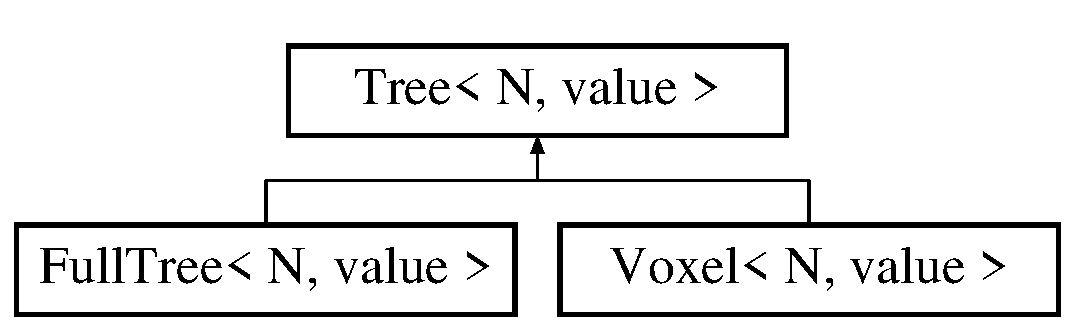
\includegraphics[height=2.000000cm]{classTree}
\end{center}
\end{figure}
\subsection*{Public Member Functions}
\begin{DoxyCompactItemize}
\item 
\mbox{\hyperlink{classTree_afd632b8d5a32c34865a305830558e256}{Tree}} (\mbox{\hyperlink{definitions_8h_aedc0ad84d1e764530814f57ad931d02a}{real}} $\ast$length, \mbox{\hyperlink{definitions_8h_aedc0ad84d1e764530814f57ad931d02a}{real}} $\ast$coords, \mbox{\hyperlink{definitions_8h_a69aa29b598b851b0640aa225a9e5d61d}{uint}} nx, \mbox{\hyperlink{definitions_8h_a69aa29b598b851b0640aa225a9e5d61d}{uint}} ny, \mbox{\hyperlink{definitions_8h_a69aa29b598b851b0640aa225a9e5d61d}{uint}} nz)
\item 
\mbox{\hyperlink{classTree_a6a43d80aaf3b7949cc412683161ef099}{Tree}} (\mbox{\hyperlink{definitions_8h_aedc0ad84d1e764530814f57ad931d02a}{real}} $\ast$length, \mbox{\hyperlink{definitions_8h_aedc0ad84d1e764530814f57ad931d02a}{real}} $\ast$coords)
\item 
\mbox{\hyperlink{classTree_a1435fce46bded38e5de4b1d5a1e1aca2}{Tree}} ()
\item 
void \mbox{\hyperlink{classTree_a56922413af6789f6ca5f64e110dc269b}{construct}} (\mbox{\hyperlink{definitions_8h_aedc0ad84d1e764530814f57ad931d02a}{real}} $\ast$length, \mbox{\hyperlink{definitions_8h_aedc0ad84d1e764530814f57ad931d02a}{real}} $\ast$coords, \mbox{\hyperlink{definitions_8h_a69aa29b598b851b0640aa225a9e5d61d}{uint}} nx, \mbox{\hyperlink{definitions_8h_a69aa29b598b851b0640aa225a9e5d61d}{uint}} ny, \mbox{\hyperlink{definitions_8h_a69aa29b598b851b0640aa225a9e5d61d}{uint}} nz)
\item 
virtual void \mbox{\hyperlink{classTree_a01f065cafedac5e2845e9d17bf87b783}{level}} (\mbox{\hyperlink{definitions_8h_af8682350bd8bb38ee9023f7a0a310add}{morton}}$<$ N $>$ key, \mbox{\hyperlink{definitions_8h_a69aa29b598b851b0640aa225a9e5d61d}{uint}} $\ast$level)
\item 
void \mbox{\hyperlink{classTree_aea583de3932917fd2cfbcd2d09318363}{centroid}} (\mbox{\hyperlink{definitions_8h_af8682350bd8bb38ee9023f7a0a310add}{morton}}$<$ N $>$ key, \mbox{\hyperlink{definitions_8h_aedc0ad84d1e764530814f57ad931d02a}{real}} $\ast$xyz)
\item 
void \mbox{\hyperlink{classTree_a9be1d9b3344d8c7300bc600e4d959ef1}{enclosing\+Box}} (\mbox{\hyperlink{definitions_8h_af8682350bd8bb38ee9023f7a0a310add}{morton}}$<$ N $>$ key, \mbox{\hyperlink{definitions_8h_aedc0ad84d1e764530814f57ad931d02a}{real}} $\ast$X)
\item 
virtual \mbox{\hyperlink{definitions_8h_acf2396ef4de9eb8a6324b9f1a624ea85}{bitmap}}$<$ N, value $>$\+::iterator \mbox{\hyperlink{classTree_aa9a32f0e006ee027c037669b8b1c7d01}{begin}} ()
\item 
virtual \mbox{\hyperlink{definitions_8h_acf2396ef4de9eb8a6324b9f1a624ea85}{bitmap}}$<$ N, value $>$\+::iterator \mbox{\hyperlink{classTree_a780c144c3fa4f648e7c616d7010721b0}{end}} ()
\item 
virtual \mbox{\hyperlink{definitions_8h_a69aa29b598b851b0640aa225a9e5d61d}{uint}} \mbox{\hyperlink{classTree_a8af31c93aa821f0d853e920bcba1829a}{size}} ()
\item 
void \mbox{\hyperlink{classTree_aca5c23bba3aa776b573e4f81d3ada031}{reserve}} (\mbox{\hyperlink{definitions_8h_a69aa29b598b851b0640aa225a9e5d61d}{uint}} $\ast$reservedsize)
\item 
void \mbox{\hyperlink{classTree_a33f60f27d0cf871b68bf2ed82638d1c7}{siblings}} (\mbox{\hyperlink{definitions_8h_af8682350bd8bb38ee9023f7a0a310add}{morton}}$<$ N $>$ key, \mbox{\hyperlink{definitions_8h_a69aa29b598b851b0640aa225a9e5d61d}{uint}} mylevel, \mbox{\hyperlink{definitions_8h_af8682350bd8bb38ee9023f7a0a310add}{morton}}$<$ N $>$ $\ast$sibkey)
\item 
void \mbox{\hyperlink{classTree_af2b416c08ae9132bfd466fe3fa288033}{refine}} (\mbox{\hyperlink{definitions_8h_af8682350bd8bb38ee9023f7a0a310add}{morton}}$<$ N $>$ key)
\item 
void \mbox{\hyperlink{classTree_ab570c49c859bb12ab22f29eb1fb51e0f}{derefine}} (\mbox{\hyperlink{definitions_8h_af8682350bd8bb38ee9023f7a0a310add}{morton}}$<$ N $>$ key)
\item 
void \mbox{\hyperlink{classTree_a4b8830fdf12cdd981a853937b6289816}{refine\+Refine\+List}} ()
\item 
void \mbox{\hyperlink{classTree_a44a82b0e29d139138605cd55427bb0bd}{refine\+Refine\+List}} (\mbox{\hyperlink{definitions_8h_a55821d7929f3f16aaf1466129c209492}{bitvector}}$<$ N $>$ \&V)
\item 
void \mbox{\hyperlink{classTree_a79d852515f810c7d67d3b8f7d157a03b}{four\+To\+OneP}} (\mbox{\hyperlink{definitions_8h_a69aa29b598b851b0640aa225a9e5d61d}{uint}} istart, \mbox{\hyperlink{definitions_8h_a69aa29b598b851b0640aa225a9e5d61d}{uint}} iend)
\item 
void \mbox{\hyperlink{classTree_a5e5fe24ceea87aeaa4931eb770e63484}{refine\+Refine\+List}} (\mbox{\hyperlink{definitions_8h_a69aa29b598b851b0640aa225a9e5d61d}{uint}} istart, \mbox{\hyperlink{definitions_8h_a69aa29b598b851b0640aa225a9e5d61d}{uint}} iend)
\item 
void \mbox{\hyperlink{classTree_a645682dbe12c75b89752e94b4c13faa4}{four\+To\+One}} ()
\item 
void \mbox{\hyperlink{classTree_a272d3af67b3ab350755281bba8d4e18c}{find\+Flip\+Level}} (\mbox{\hyperlink{definitions_8h_af8682350bd8bb38ee9023f7a0a310add}{morton}}$<$ N $>$ key, \mbox{\hyperlink{definitions_8h_a69aa29b598b851b0640aa225a9e5d61d}{uint}} $\ast$mylevel, \mbox{\hyperlink{definitions_8h_a69aa29b598b851b0640aa225a9e5d61d}{uint}} $\ast$changedirectionlevel, \mbox{\hyperlink{definitions_8h_a69aa29b598b851b0640aa225a9e5d61d}{uint}} $\ast$direction)
\item 
void \mbox{\hyperlink{classTree_add6b161eec89fc2a372f3e2f46862a98}{flip\+For\+Nbr}} (\mbox{\hyperlink{definitions_8h_af8682350bd8bb38ee9023f7a0a310add}{morton}}$<$ N $>$ $\ast$key, \mbox{\hyperlink{definitions_8h_a69aa29b598b851b0640aa225a9e5d61d}{uint}} $\ast$mylevel, \mbox{\hyperlink{definitions_8h_a69aa29b598b851b0640aa225a9e5d61d}{uint}} $\ast$changedirectionlevel, \mbox{\hyperlink{definitions_8h_a69aa29b598b851b0640aa225a9e5d61d}{uint}} $\ast$direction)
\item 
\mbox{\hyperlink{definitions_8h_a69aa29b598b851b0640aa225a9e5d61d}{uint}} \mbox{\hyperlink{classTree_a4bc3620d378608937e528270745f435e}{Is\+In\+Vector\+List}} (\mbox{\hyperlink{definitions_8h_af8682350bd8bb38ee9023f7a0a310add}{morton}}$<$ N $>$ key)
\item 
void \mbox{\hyperlink{classTree_a87d766216a59c8c77207f0fa2d093676}{add\+To\+List}} (\mbox{\hyperlink{definitions_8h_af8682350bd8bb38ee9023f7a0a310add}{morton}}$<$ N $>$ key)
\item 
\mbox{\hyperlink{definitions_8h_a69aa29b598b851b0640aa225a9e5d61d}{uint}} \mbox{\hyperlink{classTree_a5304383e6a6fea724e6ad4c8f5c4b754}{count}} (\mbox{\hyperlink{definitions_8h_af8682350bd8bb38ee9023f7a0a310add}{morton}}$<$ N $>$ key)
\item 
void \mbox{\hyperlink{classTree_a4527b5986587bad066e10ea733c1bc95}{add\+To\+Derefine\+List}} (\mbox{\hyperlink{definitions_8h_af8682350bd8bb38ee9023f7a0a310add}{morton}}$<$ N $>$ key)
\begin{DoxyCompactList}\small\item\em If any of the siblings are listed in the dereffinement do not add to the list as derefining one child means removing all the siblings. \end{DoxyCompactList}\item 
void \mbox{\hyperlink{classTree_a09d2a574f82bfd4e8f7974a6a3fda540}{derefine\+Derefine\+List}} (\mbox{\hyperlink{definitions_8h_a69aa29b598b851b0640aa225a9e5d61d}{uint}} nlevel)
\item 
\mbox{\hyperlink{definitions_8h_a69aa29b598b851b0640aa225a9e5d61d}{uint}} \mbox{\hyperlink{classTree_a2ef8077c21a8972b1ea126ec2fb9d4a5}{is\+Inside\+Solid}} (const \mbox{\hyperlink{definitions_8h_af8682350bd8bb38ee9023f7a0a310add}{morton}}$<$ N $>$ key, const \mbox{\hyperlink{definitions_8h_aedc0ad84d1e764530814f57ad931d02a}{real}} $\ast$geom\+\_\+xyz, \mbox{\hyperlink{definitions_8h_a69aa29b598b851b0640aa225a9e5d61d}{uint}} n)
\item 
virtual \mbox{\hyperlink{definitions_8h_acf2396ef4de9eb8a6324b9f1a624ea85}{bitmap}}$<$ N, value $>$\+::iterator \mbox{\hyperlink{classTree_a8337d6639f90ef96e4d42e1cbfab61dd}{find}} (\mbox{\hyperlink{definitions_8h_af8682350bd8bb38ee9023f7a0a310add}{morton}}$<$ N $>$ key)
\item 
void \mbox{\hyperlink{classTree_a5636d1c76405db54820d900909161987}{insert\+Key}} (\mbox{\hyperlink{definitions_8h_af8682350bd8bb38ee9023f7a0a310add}{morton}}$<$ N $>$ key)
\item 
void \mbox{\hyperlink{classTree_a799cfd84de5609b6a89284f116f03cfd}{convert\+Stl2\+Morton}} (\mbox{\hyperlink{definitions_8h_a69aa29b598b851b0640aa225a9e5d61d}{uint}} geom\+\_\+size, \mbox{\hyperlink{definitions_8h_aedc0ad84d1e764530814f57ad931d02a}{real}} $\ast$geom\+\_\+xyz)
\item 
void \mbox{\hyperlink{classTree_a9ba1d0e46c90f677fb33480f3061624b}{push\+To\+Refinelist}} (\mbox{\hyperlink{definitions_8h_a69aa29b598b851b0640aa225a9e5d61d}{uint}} \mbox{\hyperlink{classTree_a01f065cafedac5e2845e9d17bf87b783}{level}})
\item 
bool \mbox{\hyperlink{classTree_a48d8a704bb776cb9720e53b4e849abc5}{is\+Boundary}} (\mbox{\hyperlink{definitions_8h_af8682350bd8bb38ee9023f7a0a310add}{morton}}$<$ N $>$ \&key)
\item 
void \mbox{\hyperlink{classTree_afe37f37ae3c392c4df2abdf07dd7c5a3}{extract\+Boundary}} ()
\item 
void \mbox{\hyperlink{classTree_affd94b8b250ab921a02f987977c0b14c}{get\+Directions}} (\mbox{\hyperlink{definitions_8h_af8682350bd8bb38ee9023f7a0a310add}{morton}}$<$ N $>$ \&key, vector$<$ \mbox{\hyperlink{definitions_8h_a69aa29b598b851b0640aa225a9e5d61d}{uint}} $>$ \&directions)
\item 
\mbox{\hyperlink{definitions_8h_a69aa29b598b851b0640aa225a9e5d61d}{uint}} \mbox{\hyperlink{classTree_a214243106c17c81d193834cfeb7dfd85}{refine\+List\+Size}} ()
\item 
void \mbox{\hyperlink{classTree_ad047a737bb54fe039333c284f80994df}{clear\+Refine\+List}} ()
\item 
void \mbox{\hyperlink{classTree_a9e107129872bf20de6ea619136a74929}{extract\+BoundaryP}} (\mbox{\hyperlink{definitions_8h_a69aa29b598b851b0640aa225a9e5d61d}{uint}} istart, \mbox{\hyperlink{definitions_8h_a69aa29b598b851b0640aa225a9e5d61d}{uint}} iend)
\item 
bool \mbox{\hyperlink{classTree_af672673619621aa27e5e0c35dd3449d2}{is\+In\+Mesh\+List}} (const \mbox{\hyperlink{definitions_8h_af8682350bd8bb38ee9023f7a0a310add}{morton}}$<$ N $>$ \&key)
\item 
bool \mbox{\hyperlink{classTree_a78d174e942a78fa20ac98db8c98ae6be}{is\+In\+Refine\+List}} (const \mbox{\hyperlink{definitions_8h_af8682350bd8bb38ee9023f7a0a310add}{morton}}$<$ N $>$ \&key)
\item 
void \mbox{\hyperlink{classTree_abe71f9daa0c90b01a9144ade766c500f}{construct\+Higher\+Level\+Nbrs}} (const \mbox{\hyperlink{definitions_8h_af8682350bd8bb38ee9023f7a0a310add}{morton}}$<$ N $>$ \&key, const \mbox{\hyperlink{definitions_8h_a69aa29b598b851b0640aa225a9e5d61d}{uint}} \&keylevel, const \mbox{\hyperlink{definitions_8h_a69aa29b598b851b0640aa225a9e5d61d}{uint}} \&direction, \mbox{\hyperlink{definitions_8h_af8682350bd8bb38ee9023f7a0a310add}{morton}}$<$ N $>$ $\ast$nbr)
\item 
void \mbox{\hyperlink{classTree_a76dbe79f57a7f640a6427f4bb4c4adef}{print\+Mesh}} ()
\item 
bool \mbox{\hyperlink{classTree_a1fc56044946bc23f6c31c103c30d25fa}{is\+Boundary}} (const \mbox{\hyperlink{definitions_8h_af8682350bd8bb38ee9023f7a0a310add}{morton}}$<$ N $>$ \&key, \mbox{\hyperlink{definitions_8h_a69aa29b598b851b0640aa225a9e5d61d}{uint}} direction)
\item 
std\+::pair$<$ \mbox{\hyperlink{definitions_8h_af8682350bd8bb38ee9023f7a0a310add}{morton}}$<$ N $>$, int $>$ \mbox{\hyperlink{classTree_ae4cedc682194265e242bc37bc3df1386}{read\+Refine\+List}} (typename std\+::unordered\+\_\+map$<$ \mbox{\hyperlink{definitions_8h_af8682350bd8bb38ee9023f7a0a310add}{morton}}$<$ N $>$, int $>$\+::iterator it)
\item 
\mbox{\hyperlink{definitions_8h_af8682350bd8bb38ee9023f7a0a310add}{morton}}$<$ N $>$ \mbox{\hyperlink{classTree_acc8f2387fd43e2d148c7a800eddd0c31}{read\+Derefine\+List}} (typename std\+::unordered\+\_\+map$<$ \mbox{\hyperlink{definitions_8h_af8682350bd8bb38ee9023f7a0a310add}{morton}}$<$ N $>$, int $>$\+::iterator it)
\item 
void \mbox{\hyperlink{classTree_a7c243257bc4cbe0cec0d5b1a2098782c}{get\+Key}} (\mbox{\hyperlink{definitions_8h_a69aa29b598b851b0640aa225a9e5d61d}{uint}} i, \mbox{\hyperlink{definitions_8h_af8682350bd8bb38ee9023f7a0a310add}{morton}}$<$ N $>$ \&key)
\item 
void \mbox{\hyperlink{classTree_a2c51dee6b6d3a07a38fbd465adab62f8}{clear\+Morton\+S\+TL}} ()
\item 
void \mbox{\hyperlink{classTree_a017dbf01d574294edbd8e9003e8d0002}{retain\+Four\+To\+One}} ()
\item 
void \mbox{\hyperlink{classTree_a69539d7a5eb07c519460846207b50ae8}{remove\+From\+Derefine\+List}} (typename std\+::unordered\+\_\+map$<$ \mbox{\hyperlink{definitions_8h_af8682350bd8bb38ee9023f7a0a310add}{morton}}$<$ N $>$, int $>$\+::iterator it)
\item 
unordered\+\_\+map$<$ \mbox{\hyperlink{definitions_8h_af8682350bd8bb38ee9023f7a0a310add}{morton}}$<$ N $>$, int $>$\+::iterator \mbox{\hyperlink{classTree_aba8489b0b3498e5995e1ab0fc6a7fbab}{Dbegin}} ()
\item 
unordered\+\_\+map$<$ \mbox{\hyperlink{definitions_8h_af8682350bd8bb38ee9023f7a0a310add}{morton}}$<$ N $>$, int $>$\+::iterator \mbox{\hyperlink{classTree_a89894433bb64a326f411f328890b187a}{Dend}} ()
\item 
void \mbox{\hyperlink{classTree_ac151fd0d1ed04e995d03d3cc6b5f7237}{derefine\+Derefine\+List}} ()
\item 
void \mbox{\hyperlink{classTree_a3dab87d8315821f5ee2cc20a1b80c393}{clear\+Mesh}} ()
\item 
void \mbox{\hyperlink{classTree_a52c75138e39fc5ee1cb034b3ef3d9b97}{push\+To\+Derefinelist}} (\mbox{\hyperlink{definitions_8h_a69aa29b598b851b0640aa225a9e5d61d}{uint}} nlevel)
\item 
unordered\+\_\+map$<$ \mbox{\hyperlink{definitions_8h_af8682350bd8bb38ee9023f7a0a310add}{morton}}$<$ N $>$, int $>$\+::iterator \mbox{\hyperlink{classTree_aac90381448bee888a44fb8089023d0d8}{Rbegin}} ()
\item 
unordered\+\_\+map$<$ \mbox{\hyperlink{definitions_8h_af8682350bd8bb38ee9023f7a0a310add}{morton}}$<$ N $>$, int $>$\+::iterator \mbox{\hyperlink{classTree_aa3414a027171fb07f8f4b9acb0699d9a}{Rend}} ()
\item 
std\+::unordered\+\_\+map$<$ \mbox{\hyperlink{definitions_8h_af8682350bd8bb38ee9023f7a0a310add}{morton}}$<$ N $>$, int $>$\+::iterator \mbox{\hyperlink{classTree_a7844a0ee00798d6058e7a741cfe0e85b}{find\+In\+Derefine}} (\mbox{\hyperlink{definitions_8h_af8682350bd8bb38ee9023f7a0a310add}{morton}}$<$ N $>$ key)
\item 
void \mbox{\hyperlink{classTree_ad5d7ea8995c06e23b58f1ba00403427c}{morton\+S\+T\+Lclear}} ()
\item 
void \mbox{\hyperlink{classTree_a77e16d7a249bca09cf3deff800b85789}{flip\+Refine\+Elem\+Tag}} (typename std\+::unordered\+\_\+map$<$ \mbox{\hyperlink{definitions_8h_af8682350bd8bb38ee9023f7a0a310add}{morton}}$<$ N $>$, int $>$\+::iterator it)
\item 
void \mbox{\hyperlink{classTree_aa07840353d0eb24fe3af3ddf348f3378}{refinelist\+Reset}} ()
\item 
void \mbox{\hyperlink{classTree_ab93adb07d37664f0e359eb8ea9cf56d1}{construct\+Nonlocal\+Higher\+Level\+Nbrs}} (const \mbox{\hyperlink{definitions_8h_af8682350bd8bb38ee9023f7a0a310add}{morton}}$<$ N $>$ \&key, const \mbox{\hyperlink{definitions_8h_a69aa29b598b851b0640aa225a9e5d61d}{uint}} \&keylevel, const \mbox{\hyperlink{definitions_8h_a69aa29b598b851b0640aa225a9e5d61d}{uint}} \&direction, \mbox{\hyperlink{definitions_8h_af8682350bd8bb38ee9023f7a0a310add}{morton}}$<$ N $>$ $\ast$nbr)
\item 
void \mbox{\hyperlink{classTree_a9e11471977b8d0079c204b858357f339}{insert\+Seed}} (\mbox{\hyperlink{definitions_8h_af8682350bd8bb38ee9023f7a0a310add}{morton}}$<$ N $>$ \&key)
\item 
void \mbox{\hyperlink{classTree_acbedf93a6977d60abc4f08c789c7c30e}{insert\+Nbrs}} (vector$<$ int $>$ \&Nbrs)
\item 
void \mbox{\hyperlink{classTree_a49dcce2706c8e330950ac362826c3a9d}{enclosing\+Box\+Fixed\+Level}} (\mbox{\hyperlink{definitions_8h_af8682350bd8bb38ee9023f7a0a310add}{morton}}$<$ N $>$ key, \mbox{\hyperlink{definitions_8h_a69aa29b598b851b0640aa225a9e5d61d}{uint}} mylevel, \mbox{\hyperlink{definitions_8h_aedc0ad84d1e764530814f57ad931d02a}{real}} $\ast$X)
\item 
void \mbox{\hyperlink{classTree_a50c5721c4b9535029e4700419bec234c}{centroid\+Fixed\+Level}} (\mbox{\hyperlink{definitions_8h_af8682350bd8bb38ee9023f7a0a310add}{morton}}$<$ N $>$ key, const \mbox{\hyperlink{definitions_8h_a69aa29b598b851b0640aa225a9e5d61d}{uint}} mylevel, \mbox{\hyperlink{definitions_8h_aedc0ad84d1e764530814f57ad931d02a}{real}} $\ast$xyz)
\item 
virtual void \mbox{\hyperlink{classTree_a945d137d27bb55d9feb5762ac821572a}{convert\+Coord\+To\+Morton}} (\mbox{\hyperlink{definitions_8h_aedc0ad84d1e764530814f57ad931d02a}{real}} $\ast$xyz, \mbox{\hyperlink{definitions_8h_af8682350bd8bb38ee9023f7a0a310add}{morton}}$<$ N $>$ \&key)
\item 
std\+::unordered\+\_\+map$<$ \mbox{\hyperlink{definitions_8h_af8682350bd8bb38ee9023f7a0a310add}{morton}}$<$ N $>$, int $>$\+::iterator \mbox{\hyperlink{classTree_a9462adc7e7806404cc1b75d9a26894ae}{find\+In\+List}} (\mbox{\hyperlink{definitions_8h_af8682350bd8bb38ee9023f7a0a310add}{morton}}$<$ N $>$ key)
\item 
\mbox{\hyperlink{classTree_afcec6e88f6434550c3abf3185a25ff53}{$\sim$\+Tree}} ()
\end{DoxyCompactItemize}
\subsection*{Public Attributes}
\begin{DoxyCompactItemize}
\item 
\mbox{\hyperlink{definitions_8h_a55821d7929f3f16aaf1466129c209492}{bitvector}}$<$ N $>$ \mbox{\hyperlink{classTree_aa9c837fabf42230cfd53775130886cc6}{boundarylist}}
\end{DoxyCompactItemize}
\subsection*{Protected Attributes}
\begin{DoxyCompactItemize}
\item 
\mbox{\hyperlink{definitions_8h_aedc0ad84d1e764530814f57ad931d02a}{real}} \mbox{\hyperlink{classTree_a6dd200497bd886db369d621cc05af09f}{ancestorlength}} \mbox{[}3\mbox{]}
\item 
\mbox{\hyperlink{definitions_8h_aedc0ad84d1e764530814f57ad931d02a}{real}} \mbox{\hyperlink{classTree_a2199b0f2221e9bac89bbf57ac1fef24e}{ancestorcoords}} \mbox{[}3\mbox{]}
\item 
\mbox{\hyperlink{definitions_8h_af8682350bd8bb38ee9023f7a0a310add}{morton}}$<$ N $>$ \mbox{\hyperlink{classTree_a8b6e0e406bcbfc2b8e1598cfc967e6c8}{ancestorkey}} = 0
\item 
\mbox{\hyperlink{definitions_8h_a69aa29b598b851b0640aa225a9e5d61d}{uint}} \mbox{\hyperlink{classTree_a18a47db1dd6763090994bfe28d89b8f6}{npx}}
\item 
\mbox{\hyperlink{definitions_8h_a69aa29b598b851b0640aa225a9e5d61d}{uint}} \mbox{\hyperlink{classTree_af436baa75e35a4786a377b6fe237c5e0}{npy}}
\item 
\mbox{\hyperlink{definitions_8h_a69aa29b598b851b0640aa225a9e5d61d}{uint}} \mbox{\hyperlink{classTree_a0b132f3e84c33e27e1f78f0542081e7b}{npz}}
\end{DoxyCompactItemize}
\subsection*{Private Attributes}
\begin{DoxyCompactItemize}
\item 
\mbox{\hyperlink{definitions_8h_acf2396ef4de9eb8a6324b9f1a624ea85}{bitmap}}$<$ N, value $>$ \mbox{\hyperlink{classTree_a2baee1e4878452eac675671775360145}{mesh}}
\item 
std\+::unordered\+\_\+map$<$ \mbox{\hyperlink{definitions_8h_af8682350bd8bb38ee9023f7a0a310add}{morton}}$<$ N $>$, int $>$ \mbox{\hyperlink{classTree_a2fbb2b9ed44f73aa10192eab2a9d126b}{refinelist}}
\item 
\mbox{\hyperlink{definitions_8h_a55821d7929f3f16aaf1466129c209492}{bitvector}}$<$ N $>$ \mbox{\hyperlink{classTree_ab97dba8fe7958a363ff7eac2f8199dba}{morton\+S\+TL}}
\item 
std\+::unordered\+\_\+map$<$ \mbox{\hyperlink{definitions_8h_af8682350bd8bb38ee9023f7a0a310add}{morton}}$<$ N $>$, int $>$ \mbox{\hyperlink{classTree_acfb17b257f964def045244fbd73f8c6c}{derefinelist}}
\end{DoxyCompactItemize}
\subsection*{Friends}
\begin{DoxyCompactItemize}
\item 
{\footnotesize template$<$size\+\_\+t N1, typename value2 $>$ }\\class \mbox{\hyperlink{classTree_ab87a301be23011123f58ee948a55b2d9}{Hdf5\+Xmf}}
\end{DoxyCompactItemize}


\subsection{Detailed Description}
\subsubsection*{template$<$size\+\_\+t N, typename value$>$\newline
class Tree$<$ N, value $>$}

This Class Generates a 4\+:1 balancerd A\+MR mesh. 

\subsection{Constructor \& Destructor Documentation}
\mbox{\Hypertarget{classTree_afd632b8d5a32c34865a305830558e256}\label{classTree_afd632b8d5a32c34865a305830558e256}} 
\index{Tree@{Tree}!Tree@{Tree}}
\index{Tree@{Tree}!Tree@{Tree}}
\subsubsection{\texorpdfstring{Tree()}{Tree()}\hspace{0.1cm}{\footnotesize\ttfamily [1/3]}}
{\footnotesize\ttfamily template$<$size\+\_\+t N, typename value $>$ \\
\mbox{\hyperlink{classTree}{Tree}}$<$ N, value $>$\+::\mbox{\hyperlink{classTree}{Tree}} (\begin{DoxyParamCaption}\item[{\mbox{\hyperlink{definitions_8h_aedc0ad84d1e764530814f57ad931d02a}{real}} $\ast$}]{length,  }\item[{\mbox{\hyperlink{definitions_8h_aedc0ad84d1e764530814f57ad931d02a}{real}} $\ast$}]{coords,  }\item[{\mbox{\hyperlink{definitions_8h_a69aa29b598b851b0640aa225a9e5d61d}{uint}}}]{nx,  }\item[{\mbox{\hyperlink{definitions_8h_a69aa29b598b851b0640aa225a9e5d61d}{uint}}}]{ny,  }\item[{\mbox{\hyperlink{definitions_8h_a69aa29b598b851b0640aa225a9e5d61d}{uint}}}]{nz }\end{DoxyParamCaption})}

constructor \mbox{\Hypertarget{classTree_a6a43d80aaf3b7949cc412683161ef099}\label{classTree_a6a43d80aaf3b7949cc412683161ef099}} 
\index{Tree@{Tree}!Tree@{Tree}}
\index{Tree@{Tree}!Tree@{Tree}}
\subsubsection{\texorpdfstring{Tree()}{Tree()}\hspace{0.1cm}{\footnotesize\ttfamily [2/3]}}
{\footnotesize\ttfamily template$<$size\+\_\+t N, typename value $>$ \\
\mbox{\hyperlink{classTree}{Tree}}$<$ N, value $>$\+::\mbox{\hyperlink{classTree}{Tree}} (\begin{DoxyParamCaption}\item[{\mbox{\hyperlink{definitions_8h_aedc0ad84d1e764530814f57ad931d02a}{real}} $\ast$}]{length,  }\item[{\mbox{\hyperlink{definitions_8h_aedc0ad84d1e764530814f57ad931d02a}{real}} $\ast$}]{coords }\end{DoxyParamCaption})}

constructor \mbox{\Hypertarget{classTree_a1435fce46bded38e5de4b1d5a1e1aca2}\label{classTree_a1435fce46bded38e5de4b1d5a1e1aca2}} 
\index{Tree@{Tree}!Tree@{Tree}}
\index{Tree@{Tree}!Tree@{Tree}}
\subsubsection{\texorpdfstring{Tree()}{Tree()}\hspace{0.1cm}{\footnotesize\ttfamily [3/3]}}
{\footnotesize\ttfamily template$<$size\+\_\+t N, typename value$>$ \\
\mbox{\hyperlink{classTree}{Tree}}$<$ N, value $>$\+::\mbox{\hyperlink{classTree}{Tree}} (\begin{DoxyParamCaption}{ }\end{DoxyParamCaption})\hspace{0.3cm}{\ttfamily [inline]}}

\mbox{\Hypertarget{classTree_afcec6e88f6434550c3abf3185a25ff53}\label{classTree_afcec6e88f6434550c3abf3185a25ff53}} 
\index{Tree@{Tree}!````~Tree@{$\sim$\+Tree}}
\index{````~Tree@{$\sim$\+Tree}!Tree@{Tree}}
\subsubsection{\texorpdfstring{$\sim$\+Tree()}{~Tree()}}
{\footnotesize\ttfamily template$<$size\+\_\+t N, typename value $>$ \\
\mbox{\hyperlink{classTree}{Tree}}$<$ N, value $>$\+::$\sim$\mbox{\hyperlink{classTree}{Tree}} (\begin{DoxyParamCaption}{ }\end{DoxyParamCaption})}

Destructor of the class, it frees the memeory pointed by pointer in the hashmap value if allocated 

\subsection{Member Function Documentation}
\mbox{\Hypertarget{classTree_a4527b5986587bad066e10ea733c1bc95}\label{classTree_a4527b5986587bad066e10ea733c1bc95}} 
\index{Tree@{Tree}!add\+To\+Derefine\+List@{add\+To\+Derefine\+List}}
\index{add\+To\+Derefine\+List@{add\+To\+Derefine\+List}!Tree@{Tree}}
\subsubsection{\texorpdfstring{add\+To\+Derefine\+List()}{addToDerefineList()}}
{\footnotesize\ttfamily template$<$size\+\_\+t N, typename value $>$ \\
void \mbox{\hyperlink{classTree}{Tree}}$<$ N, value $>$\+::add\+To\+Derefine\+List (\begin{DoxyParamCaption}\item[{\mbox{\hyperlink{definitions_8h_af8682350bd8bb38ee9023f7a0a310add}{morton}}$<$ N $>$}]{key }\end{DoxyParamCaption})}



If any of the siblings are listed in the dereffinement do not add to the list as derefining one child means removing all the siblings. 

adds the element to derefinelist \mbox{\Hypertarget{classTree_a87d766216a59c8c77207f0fa2d093676}\label{classTree_a87d766216a59c8c77207f0fa2d093676}} 
\index{Tree@{Tree}!add\+To\+List@{add\+To\+List}}
\index{add\+To\+List@{add\+To\+List}!Tree@{Tree}}
\subsubsection{\texorpdfstring{add\+To\+List()}{addToList()}}
{\footnotesize\ttfamily template$<$size\+\_\+t N, typename value $>$ \\
void \mbox{\hyperlink{classTree}{Tree}}$<$ N, value $>$\+::add\+To\+List (\begin{DoxyParamCaption}\item[{\mbox{\hyperlink{definitions_8h_af8682350bd8bb38ee9023f7a0a310add}{morton}}$<$ N $>$}]{key }\end{DoxyParamCaption})}

adds element to refinelist \mbox{\Hypertarget{classTree_aa9a32f0e006ee027c037669b8b1c7d01}\label{classTree_aa9a32f0e006ee027c037669b8b1c7d01}} 
\index{Tree@{Tree}!begin@{begin}}
\index{begin@{begin}!Tree@{Tree}}
\subsubsection{\texorpdfstring{begin()}{begin()}}
{\footnotesize\ttfamily template$<$size\+\_\+t N, typename value $>$ \\
\mbox{\hyperlink{definitions_8h_acf2396ef4de9eb8a6324b9f1a624ea85}{bitmap}}$<$ N, value $>$\+::iterator \mbox{\hyperlink{classTree}{Tree}}$<$ N, value $>$\+::begin (\begin{DoxyParamCaption}{ }\end{DoxyParamCaption})\hspace{0.3cm}{\ttfamily [virtual]}}

iterator returning the first object 

Reimplemented in \mbox{\hyperlink{classFullTree_af2fbecbd352a329634a6fdc35f519968}{Full\+Tree$<$ N, value $>$}}.

\mbox{\Hypertarget{classTree_aea583de3932917fd2cfbcd2d09318363}\label{classTree_aea583de3932917fd2cfbcd2d09318363}} 
\index{Tree@{Tree}!centroid@{centroid}}
\index{centroid@{centroid}!Tree@{Tree}}
\subsubsection{\texorpdfstring{centroid()}{centroid()}}
{\footnotesize\ttfamily template$<$size\+\_\+t N, typename value $>$ \\
void \mbox{\hyperlink{classTree}{Tree}}$<$ N, value $>$\+::centroid (\begin{DoxyParamCaption}\item[{\mbox{\hyperlink{definitions_8h_af8682350bd8bb38ee9023f7a0a310add}{morton}}$<$ N $>$}]{key,  }\item[{\mbox{\hyperlink{definitions_8h_aedc0ad84d1e764530814f57ad931d02a}{real}} $\ast$}]{xyz }\end{DoxyParamCaption})}

calculates the centroid of the cube given the morton key of the element \mbox{\Hypertarget{classTree_a50c5721c4b9535029e4700419bec234c}\label{classTree_a50c5721c4b9535029e4700419bec234c}} 
\index{Tree@{Tree}!centroid\+Fixed\+Level@{centroid\+Fixed\+Level}}
\index{centroid\+Fixed\+Level@{centroid\+Fixed\+Level}!Tree@{Tree}}
\subsubsection{\texorpdfstring{centroid\+Fixed\+Level()}{centroidFixedLevel()}}
{\footnotesize\ttfamily template$<$size\+\_\+t N, typename value $>$ \\
void \mbox{\hyperlink{classTree}{Tree}}$<$ N, value $>$\+::centroid\+Fixed\+Level (\begin{DoxyParamCaption}\item[{\mbox{\hyperlink{definitions_8h_af8682350bd8bb38ee9023f7a0a310add}{morton}}$<$ N $>$}]{key,  }\item[{const \mbox{\hyperlink{definitions_8h_a69aa29b598b851b0640aa225a9e5d61d}{uint}}}]{mylevel,  }\item[{\mbox{\hyperlink{definitions_8h_aedc0ad84d1e764530814f57ad931d02a}{real}} $\ast$}]{xyz }\end{DoxyParamCaption})}

\mbox{\Hypertarget{classTree_a3dab87d8315821f5ee2cc20a1b80c393}\label{classTree_a3dab87d8315821f5ee2cc20a1b80c393}} 
\index{Tree@{Tree}!clear\+Mesh@{clear\+Mesh}}
\index{clear\+Mesh@{clear\+Mesh}!Tree@{Tree}}
\subsubsection{\texorpdfstring{clear\+Mesh()}{clearMesh()}}
{\footnotesize\ttfamily template$<$size\+\_\+t N, typename value $>$ \\
void \mbox{\hyperlink{classTree}{Tree}}$<$ N, value $>$\+::clear\+Mesh (\begin{DoxyParamCaption}{ }\end{DoxyParamCaption})}

\mbox{\Hypertarget{classTree_a2c51dee6b6d3a07a38fbd465adab62f8}\label{classTree_a2c51dee6b6d3a07a38fbd465adab62f8}} 
\index{Tree@{Tree}!clear\+Morton\+S\+TL@{clear\+Morton\+S\+TL}}
\index{clear\+Morton\+S\+TL@{clear\+Morton\+S\+TL}!Tree@{Tree}}
\subsubsection{\texorpdfstring{clear\+Morton\+S\+T\+L()}{clearMortonSTL()}}
{\footnotesize\ttfamily template$<$size\+\_\+t N, typename value $>$ \\
void \mbox{\hyperlink{classTree}{Tree}}$<$ N, value $>$\+::clear\+Morton\+S\+TL (\begin{DoxyParamCaption}{ }\end{DoxyParamCaption})}

\mbox{\Hypertarget{classTree_ad047a737bb54fe039333c284f80994df}\label{classTree_ad047a737bb54fe039333c284f80994df}} 
\index{Tree@{Tree}!clear\+Refine\+List@{clear\+Refine\+List}}
\index{clear\+Refine\+List@{clear\+Refine\+List}!Tree@{Tree}}
\subsubsection{\texorpdfstring{clear\+Refine\+List()}{clearRefineList()}}
{\footnotesize\ttfamily template$<$size\+\_\+t N, typename value $>$ \\
void \mbox{\hyperlink{classTree}{Tree}}$<$ N, value $>$\+::clear\+Refine\+List (\begin{DoxyParamCaption}{ }\end{DoxyParamCaption})}

\mbox{\Hypertarget{classTree_a56922413af6789f6ca5f64e110dc269b}\label{classTree_a56922413af6789f6ca5f64e110dc269b}} 
\index{Tree@{Tree}!construct@{construct}}
\index{construct@{construct}!Tree@{Tree}}
\subsubsection{\texorpdfstring{construct()}{construct()}}
{\footnotesize\ttfamily template$<$size\+\_\+t N, typename value $>$ \\
void \mbox{\hyperlink{classTree}{Tree}}$<$ N, value $>$\+::construct (\begin{DoxyParamCaption}\item[{\mbox{\hyperlink{definitions_8h_aedc0ad84d1e764530814f57ad931d02a}{real}} $\ast$}]{length,  }\item[{\mbox{\hyperlink{definitions_8h_aedc0ad84d1e764530814f57ad931d02a}{real}} $\ast$}]{coords,  }\item[{\mbox{\hyperlink{definitions_8h_a69aa29b598b851b0640aa225a9e5d61d}{uint}}}]{nx,  }\item[{\mbox{\hyperlink{definitions_8h_a69aa29b598b851b0640aa225a9e5d61d}{uint}}}]{ny,  }\item[{\mbox{\hyperlink{definitions_8h_a69aa29b598b851b0640aa225a9e5d61d}{uint}}}]{nz }\end{DoxyParamCaption})}

need to initialize inside forest \mbox{\Hypertarget{classTree_abe71f9daa0c90b01a9144ade766c500f}\label{classTree_abe71f9daa0c90b01a9144ade766c500f}} 
\index{Tree@{Tree}!construct\+Higher\+Level\+Nbrs@{construct\+Higher\+Level\+Nbrs}}
\index{construct\+Higher\+Level\+Nbrs@{construct\+Higher\+Level\+Nbrs}!Tree@{Tree}}
\subsubsection{\texorpdfstring{construct\+Higher\+Level\+Nbrs()}{constructHigherLevelNbrs()}}
{\footnotesize\ttfamily template$<$size\+\_\+t N, typename value $>$ \\
void \mbox{\hyperlink{classTree}{Tree}}$<$ N, value $>$\+::construct\+Higher\+Level\+Nbrs (\begin{DoxyParamCaption}\item[{const \mbox{\hyperlink{definitions_8h_af8682350bd8bb38ee9023f7a0a310add}{morton}}$<$ N $>$ \&}]{key,  }\item[{const \mbox{\hyperlink{definitions_8h_a69aa29b598b851b0640aa225a9e5d61d}{uint}} \&}]{keylevel,  }\item[{const \mbox{\hyperlink{definitions_8h_a69aa29b598b851b0640aa225a9e5d61d}{uint}} \&}]{direction,  }\item[{\mbox{\hyperlink{definitions_8h_af8682350bd8bb38ee9023f7a0a310add}{morton}}$<$ N $>$ $\ast$}]{nbr }\end{DoxyParamCaption})}

\mbox{\Hypertarget{classTree_ab93adb07d37664f0e359eb8ea9cf56d1}\label{classTree_ab93adb07d37664f0e359eb8ea9cf56d1}} 
\index{Tree@{Tree}!construct\+Nonlocal\+Higher\+Level\+Nbrs@{construct\+Nonlocal\+Higher\+Level\+Nbrs}}
\index{construct\+Nonlocal\+Higher\+Level\+Nbrs@{construct\+Nonlocal\+Higher\+Level\+Nbrs}!Tree@{Tree}}
\subsubsection{\texorpdfstring{construct\+Nonlocal\+Higher\+Level\+Nbrs()}{constructNonlocalHigherLevelNbrs()}}
{\footnotesize\ttfamily template$<$size\+\_\+t N, typename value $>$ \\
void \mbox{\hyperlink{classTree}{Tree}}$<$ N, value $>$\+::construct\+Nonlocal\+Higher\+Level\+Nbrs (\begin{DoxyParamCaption}\item[{const \mbox{\hyperlink{definitions_8h_af8682350bd8bb38ee9023f7a0a310add}{morton}}$<$ N $>$ \&}]{key,  }\item[{const \mbox{\hyperlink{definitions_8h_a69aa29b598b851b0640aa225a9e5d61d}{uint}} \&}]{keylevel,  }\item[{const \mbox{\hyperlink{definitions_8h_a69aa29b598b851b0640aa225a9e5d61d}{uint}} \&}]{direction,  }\item[{\mbox{\hyperlink{definitions_8h_af8682350bd8bb38ee9023f7a0a310add}{morton}}$<$ N $>$ $\ast$}]{nbr }\end{DoxyParamCaption})}

\mbox{\Hypertarget{classTree_a945d137d27bb55d9feb5762ac821572a}\label{classTree_a945d137d27bb55d9feb5762ac821572a}} 
\index{Tree@{Tree}!convert\+Coord\+To\+Morton@{convert\+Coord\+To\+Morton}}
\index{convert\+Coord\+To\+Morton@{convert\+Coord\+To\+Morton}!Tree@{Tree}}
\subsubsection{\texorpdfstring{convert\+Coord\+To\+Morton()}{convertCoordToMorton()}}
{\footnotesize\ttfamily template$<$size\+\_\+t N, typename value $>$ \\
void \mbox{\hyperlink{classTree}{Tree}}$<$ N, value $>$\+::convert\+Coord\+To\+Morton (\begin{DoxyParamCaption}\item[{\mbox{\hyperlink{definitions_8h_aedc0ad84d1e764530814f57ad931d02a}{real}} $\ast$}]{xyz,  }\item[{\mbox{\hyperlink{definitions_8h_af8682350bd8bb38ee9023f7a0a310add}{morton}}$<$ N $>$ \&}]{key }\end{DoxyParamCaption})\hspace{0.3cm}{\ttfamily [virtual]}}

converts coordinates of a point to morton code

!$<$ this function is to find a value given the key 

Reimplemented in \mbox{\hyperlink{classFullTree_a1b0a9b6f0f5155dd8847905ee8aa1b56}{Full\+Tree$<$ N, value $>$}}.

\mbox{\Hypertarget{classTree_a799cfd84de5609b6a89284f116f03cfd}\label{classTree_a799cfd84de5609b6a89284f116f03cfd}} 
\index{Tree@{Tree}!convert\+Stl2\+Morton@{convert\+Stl2\+Morton}}
\index{convert\+Stl2\+Morton@{convert\+Stl2\+Morton}!Tree@{Tree}}
\subsubsection{\texorpdfstring{convert\+Stl2\+Morton()}{convertStl2Morton()}}
{\footnotesize\ttfamily template$<$size\+\_\+t N, typename value $>$ \\
void \mbox{\hyperlink{classTree}{Tree}}$<$ N, value $>$\+::convert\+Stl2\+Morton (\begin{DoxyParamCaption}\item[{\mbox{\hyperlink{definitions_8h_a69aa29b598b851b0640aa225a9e5d61d}{uint}}}]{geom\+\_\+size,  }\item[{\mbox{\hyperlink{definitions_8h_aedc0ad84d1e764530814f57ad931d02a}{real}} $\ast$}]{geom\+\_\+xyz }\end{DoxyParamCaption})}

converts stl coordinates to morton and puts them in morton S\+TL

!$<$ this function is to find a value given the key \mbox{\Hypertarget{classTree_a5304383e6a6fea724e6ad4c8f5c4b754}\label{classTree_a5304383e6a6fea724e6ad4c8f5c4b754}} 
\index{Tree@{Tree}!count@{count}}
\index{count@{count}!Tree@{Tree}}
\subsubsection{\texorpdfstring{count()}{count()}}
{\footnotesize\ttfamily template$<$size\+\_\+t N, typename value $>$ \\
\mbox{\hyperlink{definitions_8h_a69aa29b598b851b0640aa225a9e5d61d}{uint}} \mbox{\hyperlink{classTree}{Tree}}$<$ N, value $>$\+::count (\begin{DoxyParamCaption}\item[{\mbox{\hyperlink{definitions_8h_af8682350bd8bb38ee9023f7a0a310add}{morton}}$<$ N $>$}]{key }\end{DoxyParamCaption})}

counts the number of elements \mbox{\Hypertarget{classTree_aba8489b0b3498e5995e1ab0fc6a7fbab}\label{classTree_aba8489b0b3498e5995e1ab0fc6a7fbab}} 
\index{Tree@{Tree}!Dbegin@{Dbegin}}
\index{Dbegin@{Dbegin}!Tree@{Tree}}
\subsubsection{\texorpdfstring{Dbegin()}{Dbegin()}}
{\footnotesize\ttfamily template$<$size\+\_\+t N, typename value $>$ \\
unordered\+\_\+map$<$ \mbox{\hyperlink{definitions_8h_af8682350bd8bb38ee9023f7a0a310add}{morton}}$<$ N $>$, int $>$\+::iterator \mbox{\hyperlink{classTree}{Tree}}$<$ N, value $>$\+::Dbegin (\begin{DoxyParamCaption}{ }\end{DoxyParamCaption})}

\mbox{\Hypertarget{classTree_a89894433bb64a326f411f328890b187a}\label{classTree_a89894433bb64a326f411f328890b187a}} 
\index{Tree@{Tree}!Dend@{Dend}}
\index{Dend@{Dend}!Tree@{Tree}}
\subsubsection{\texorpdfstring{Dend()}{Dend()}}
{\footnotesize\ttfamily template$<$size\+\_\+t N, typename value $>$ \\
unordered\+\_\+map$<$ \mbox{\hyperlink{definitions_8h_af8682350bd8bb38ee9023f7a0a310add}{morton}}$<$ N $>$, int $>$\+::iterator \mbox{\hyperlink{classTree}{Tree}}$<$ N, value $>$\+::Dend (\begin{DoxyParamCaption}{ }\end{DoxyParamCaption})}

\mbox{\Hypertarget{classTree_ab570c49c859bb12ab22f29eb1fb51e0f}\label{classTree_ab570c49c859bb12ab22f29eb1fb51e0f}} 
\index{Tree@{Tree}!derefine@{derefine}}
\index{derefine@{derefine}!Tree@{Tree}}
\subsubsection{\texorpdfstring{derefine()}{derefine()}}
{\footnotesize\ttfamily template$<$size\+\_\+t N, typename value $>$ \\
void \mbox{\hyperlink{classTree}{Tree}}$<$ N, value $>$\+::derefine (\begin{DoxyParamCaption}\item[{\mbox{\hyperlink{definitions_8h_af8682350bd8bb38ee9023f7a0a310add}{morton}}$<$ N $>$}]{key }\end{DoxyParamCaption})}

if the morton code does not exist in mesh, refinement is not permitted (derefining a nonexsiting element not permitted) Also, if any of the siblings have a higher level of refinement, derefinement is ignored

$<$if the key does not exist simply igonre doing anything \mbox{\Hypertarget{classTree_a09d2a574f82bfd4e8f7974a6a3fda540}\label{classTree_a09d2a574f82bfd4e8f7974a6a3fda540}} 
\index{Tree@{Tree}!derefine\+Derefine\+List@{derefine\+Derefine\+List}}
\index{derefine\+Derefine\+List@{derefine\+Derefine\+List}!Tree@{Tree}}
\subsubsection{\texorpdfstring{derefine\+Derefine\+List()}{derefineDerefineList()}\hspace{0.1cm}{\footnotesize\ttfamily [1/2]}}
{\footnotesize\ttfamily template$<$size\+\_\+t N, typename value$>$ \\
void \mbox{\hyperlink{classTree}{Tree}}$<$ N, value $>$\+::derefine\+Derefine\+List (\begin{DoxyParamCaption}\item[{\mbox{\hyperlink{definitions_8h_a69aa29b598b851b0640aa225a9e5d61d}{uint}}}]{nlevel }\end{DoxyParamCaption})}

Derefines the mesh \mbox{\Hypertarget{classTree_ac151fd0d1ed04e995d03d3cc6b5f7237}\label{classTree_ac151fd0d1ed04e995d03d3cc6b5f7237}} 
\index{Tree@{Tree}!derefine\+Derefine\+List@{derefine\+Derefine\+List}}
\index{derefine\+Derefine\+List@{derefine\+Derefine\+List}!Tree@{Tree}}
\subsubsection{\texorpdfstring{derefine\+Derefine\+List()}{derefineDerefineList()}\hspace{0.1cm}{\footnotesize\ttfamily [2/2]}}
{\footnotesize\ttfamily template$<$size\+\_\+t N, typename value $>$ \\
void \mbox{\hyperlink{classTree}{Tree}}$<$ N, value $>$\+::derefine\+Derefine\+List (\begin{DoxyParamCaption}{ }\end{DoxyParamCaption})}

\mbox{\Hypertarget{classTree_a9be1d9b3344d8c7300bc600e4d959ef1}\label{classTree_a9be1d9b3344d8c7300bc600e4d959ef1}} 
\index{Tree@{Tree}!enclosing\+Box@{enclosing\+Box}}
\index{enclosing\+Box@{enclosing\+Box}!Tree@{Tree}}
\subsubsection{\texorpdfstring{enclosing\+Box()}{enclosingBox()}}
{\footnotesize\ttfamily template$<$size\+\_\+t N, typename value $>$ \\
void \mbox{\hyperlink{classTree}{Tree}}$<$ N, value $>$\+::enclosing\+Box (\begin{DoxyParamCaption}\item[{\mbox{\hyperlink{definitions_8h_af8682350bd8bb38ee9023f7a0a310add}{morton}}$<$ N $>$}]{key,  }\item[{\mbox{\hyperlink{definitions_8h_aedc0ad84d1e764530814f57ad931d02a}{real}} $\ast$}]{X }\end{DoxyParamCaption})}

calculates the range that an element occupies in 3D space for a given Element \mbox{\Hypertarget{classTree_a49dcce2706c8e330950ac362826c3a9d}\label{classTree_a49dcce2706c8e330950ac362826c3a9d}} 
\index{Tree@{Tree}!enclosing\+Box\+Fixed\+Level@{enclosing\+Box\+Fixed\+Level}}
\index{enclosing\+Box\+Fixed\+Level@{enclosing\+Box\+Fixed\+Level}!Tree@{Tree}}
\subsubsection{\texorpdfstring{enclosing\+Box\+Fixed\+Level()}{enclosingBoxFixedLevel()}}
{\footnotesize\ttfamily template$<$size\+\_\+t N, typename value $>$ \\
void \mbox{\hyperlink{classTree}{Tree}}$<$ N, value $>$\+::enclosing\+Box\+Fixed\+Level (\begin{DoxyParamCaption}\item[{\mbox{\hyperlink{definitions_8h_af8682350bd8bb38ee9023f7a0a310add}{morton}}$<$ N $>$}]{key,  }\item[{\mbox{\hyperlink{definitions_8h_a69aa29b598b851b0640aa225a9e5d61d}{uint}}}]{mylevel,  }\item[{\mbox{\hyperlink{definitions_8h_aedc0ad84d1e764530814f57ad931d02a}{real}} $\ast$}]{X }\end{DoxyParamCaption})}

\mbox{\Hypertarget{classTree_a780c144c3fa4f648e7c616d7010721b0}\label{classTree_a780c144c3fa4f648e7c616d7010721b0}} 
\index{Tree@{Tree}!end@{end}}
\index{end@{end}!Tree@{Tree}}
\subsubsection{\texorpdfstring{end()}{end()}}
{\footnotesize\ttfamily template$<$size\+\_\+t N, typename value $>$ \\
\mbox{\hyperlink{definitions_8h_acf2396ef4de9eb8a6324b9f1a624ea85}{bitmap}}$<$ N, value $>$\+::iterator \mbox{\hyperlink{classTree}{Tree}}$<$ N, value $>$\+::end (\begin{DoxyParamCaption}{ }\end{DoxyParamCaption})\hspace{0.3cm}{\ttfamily [virtual]}}

iterator returning the last object 

Reimplemented in \mbox{\hyperlink{classFullTree_a692131b057639fecdb1934b734cff1bb}{Full\+Tree$<$ N, value $>$}}.

\mbox{\Hypertarget{classTree_afe37f37ae3c392c4df2abdf07dd7c5a3}\label{classTree_afe37f37ae3c392c4df2abdf07dd7c5a3}} 
\index{Tree@{Tree}!extract\+Boundary@{extract\+Boundary}}
\index{extract\+Boundary@{extract\+Boundary}!Tree@{Tree}}
\subsubsection{\texorpdfstring{extract\+Boundary()}{extractBoundary()}}
{\footnotesize\ttfamily template$<$size\+\_\+t N, typename value $>$ \\
void \mbox{\hyperlink{classTree}{Tree}}$<$ N, value $>$\+::extract\+Boundary (\begin{DoxyParamCaption}{ }\end{DoxyParamCaption})}

\mbox{\Hypertarget{classTree_a9e107129872bf20de6ea619136a74929}\label{classTree_a9e107129872bf20de6ea619136a74929}} 
\index{Tree@{Tree}!extract\+BoundaryP@{extract\+BoundaryP}}
\index{extract\+BoundaryP@{extract\+BoundaryP}!Tree@{Tree}}
\subsubsection{\texorpdfstring{extract\+Boundary\+P()}{extractBoundaryP()}}
{\footnotesize\ttfamily template$<$size\+\_\+t N, typename value $>$ \\
void \mbox{\hyperlink{classTree}{Tree}}$<$ N, value $>$\+::extract\+BoundaryP (\begin{DoxyParamCaption}\item[{\mbox{\hyperlink{definitions_8h_a69aa29b598b851b0640aa225a9e5d61d}{uint}}}]{istart,  }\item[{\mbox{\hyperlink{definitions_8h_a69aa29b598b851b0640aa225a9e5d61d}{uint}}}]{iend }\end{DoxyParamCaption})}

\mbox{\Hypertarget{classTree_a8337d6639f90ef96e4d42e1cbfab61dd}\label{classTree_a8337d6639f90ef96e4d42e1cbfab61dd}} 
\index{Tree@{Tree}!find@{find}}
\index{find@{find}!Tree@{Tree}}
\subsubsection{\texorpdfstring{find()}{find()}}
{\footnotesize\ttfamily template$<$size\+\_\+t N, typename value $>$ \\
\mbox{\hyperlink{definitions_8h_acf2396ef4de9eb8a6324b9f1a624ea85}{bitmap}}$<$ N, value $>$\+::iterator \mbox{\hyperlink{classTree}{Tree}}$<$ N, value $>$\+::find (\begin{DoxyParamCaption}\item[{\mbox{\hyperlink{definitions_8h_af8682350bd8bb38ee9023f7a0a310add}{morton}}$<$ N $>$}]{key }\end{DoxyParamCaption})\hspace{0.3cm}{\ttfamily [virtual]}}

this function is to find a value given the key

!$<$ this function is to find a value given the key 

Reimplemented in \mbox{\hyperlink{classFullTree_ad0432afb277be83e79d33e1a748648a3}{Full\+Tree$<$ N, value $>$}}.

\mbox{\Hypertarget{classTree_a272d3af67b3ab350755281bba8d4e18c}\label{classTree_a272d3af67b3ab350755281bba8d4e18c}} 
\index{Tree@{Tree}!find\+Flip\+Level@{find\+Flip\+Level}}
\index{find\+Flip\+Level@{find\+Flip\+Level}!Tree@{Tree}}
\subsubsection{\texorpdfstring{find\+Flip\+Level()}{findFlipLevel()}}
{\footnotesize\ttfamily template$<$size\+\_\+t N, typename value $>$ \\
void \mbox{\hyperlink{classTree}{Tree}}$<$ N, value $>$\+::find\+Flip\+Level (\begin{DoxyParamCaption}\item[{\mbox{\hyperlink{definitions_8h_af8682350bd8bb38ee9023f7a0a310add}{morton}}$<$ N $>$}]{key,  }\item[{\mbox{\hyperlink{definitions_8h_a69aa29b598b851b0640aa225a9e5d61d}{uint}} $\ast$}]{mylevel,  }\item[{\mbox{\hyperlink{definitions_8h_a69aa29b598b851b0640aa225a9e5d61d}{uint}} $\ast$}]{changedirectionlevel,  }\item[{\mbox{\hyperlink{definitions_8h_a69aa29b598b851b0640aa225a9e5d61d}{uint}} $\ast$}]{direction }\end{DoxyParamCaption})}

detects the flip level, this info used in finding nonlocal neighbors \mbox{\Hypertarget{classTree_a7844a0ee00798d6058e7a741cfe0e85b}\label{classTree_a7844a0ee00798d6058e7a741cfe0e85b}} 
\index{Tree@{Tree}!find\+In\+Derefine@{find\+In\+Derefine}}
\index{find\+In\+Derefine@{find\+In\+Derefine}!Tree@{Tree}}
\subsubsection{\texorpdfstring{find\+In\+Derefine()}{findInDerefine()}}
{\footnotesize\ttfamily template$<$size\+\_\+t N, typename value $>$ \\
std\+::unordered\+\_\+map$<$ \mbox{\hyperlink{definitions_8h_af8682350bd8bb38ee9023f7a0a310add}{morton}}$<$ N $>$, int $>$\+::iterator \mbox{\hyperlink{classTree}{Tree}}$<$ N, value $>$\+::find\+In\+Derefine (\begin{DoxyParamCaption}\item[{\mbox{\hyperlink{definitions_8h_af8682350bd8bb38ee9023f7a0a310add}{morton}}$<$ N $>$}]{key }\end{DoxyParamCaption})}

Get the iterator from derefinelist 
\begin{DoxyParams}{Parameters}
{\em key} & E;iminate from derefinelist \\
\hline
\end{DoxyParams}
\mbox{\Hypertarget{classTree_a9462adc7e7806404cc1b75d9a26894ae}\label{classTree_a9462adc7e7806404cc1b75d9a26894ae}} 
\index{Tree@{Tree}!find\+In\+List@{find\+In\+List}}
\index{find\+In\+List@{find\+In\+List}!Tree@{Tree}}
\subsubsection{\texorpdfstring{find\+In\+List()}{findInList()}}
{\footnotesize\ttfamily template$<$size\+\_\+t N, typename value $>$ \\
std\+::unordered\+\_\+map$<$ \mbox{\hyperlink{definitions_8h_af8682350bd8bb38ee9023f7a0a310add}{morton}}$<$ N $>$, int $>$\+::iterator \mbox{\hyperlink{classTree}{Tree}}$<$ N, value $>$\+::find\+In\+List (\begin{DoxyParamCaption}\item[{\mbox{\hyperlink{definitions_8h_af8682350bd8bb38ee9023f7a0a310add}{morton}}$<$ N $>$}]{key }\end{DoxyParamCaption})}

!$<$ this function is to find a value given the key \mbox{\Hypertarget{classTree_add6b161eec89fc2a372f3e2f46862a98}\label{classTree_add6b161eec89fc2a372f3e2f46862a98}} 
\index{Tree@{Tree}!flip\+For\+Nbr@{flip\+For\+Nbr}}
\index{flip\+For\+Nbr@{flip\+For\+Nbr}!Tree@{Tree}}
\subsubsection{\texorpdfstring{flip\+For\+Nbr()}{flipForNbr()}}
{\footnotesize\ttfamily template$<$size\+\_\+t N, typename value $>$ \\
void \mbox{\hyperlink{classTree}{Tree}}$<$ N, value $>$\+::flip\+For\+Nbr (\begin{DoxyParamCaption}\item[{\mbox{\hyperlink{definitions_8h_af8682350bd8bb38ee9023f7a0a310add}{morton}}$<$ N $>$ $\ast$}]{key,  }\item[{\mbox{\hyperlink{definitions_8h_a69aa29b598b851b0640aa225a9e5d61d}{uint}} $\ast$}]{mylevel,  }\item[{\mbox{\hyperlink{definitions_8h_a69aa29b598b851b0640aa225a9e5d61d}{uint}} $\ast$}]{changedirectionlevel,  }\item[{\mbox{\hyperlink{definitions_8h_a69aa29b598b851b0640aa225a9e5d61d}{uint}} $\ast$}]{direction }\end{DoxyParamCaption})}

perform the actual operation to identify the nonlocal nbr \mbox{\Hypertarget{classTree_a77e16d7a249bca09cf3deff800b85789}\label{classTree_a77e16d7a249bca09cf3deff800b85789}} 
\index{Tree@{Tree}!flip\+Refine\+Elem\+Tag@{flip\+Refine\+Elem\+Tag}}
\index{flip\+Refine\+Elem\+Tag@{flip\+Refine\+Elem\+Tag}!Tree@{Tree}}
\subsubsection{\texorpdfstring{flip\+Refine\+Elem\+Tag()}{flipRefineElemTag()}}
{\footnotesize\ttfamily template$<$size\+\_\+t N, typename value $>$ \\
void \mbox{\hyperlink{classTree}{Tree}}$<$ N, value $>$\+::flip\+Refine\+Elem\+Tag (\begin{DoxyParamCaption}\item[{typename std\+::unordered\+\_\+map$<$ \mbox{\hyperlink{definitions_8h_af8682350bd8bb38ee9023f7a0a310add}{morton}}$<$ N $>$, int $>$\+::iterator}]{it }\end{DoxyParamCaption})}

\mbox{\Hypertarget{classTree_a645682dbe12c75b89752e94b4c13faa4}\label{classTree_a645682dbe12c75b89752e94b4c13faa4}} 
\index{Tree@{Tree}!four\+To\+One@{four\+To\+One}}
\index{four\+To\+One@{four\+To\+One}!Tree@{Tree}}
\subsubsection{\texorpdfstring{four\+To\+One()}{fourToOne()}}
{\footnotesize\ttfamily template$<$size\+\_\+t N, typename value $>$ \\
void \mbox{\hyperlink{classTree}{Tree}}$<$ N, value $>$\+::four\+To\+One (\begin{DoxyParamCaption}{ }\end{DoxyParamCaption})}

imposes 4\+:1 balance given the list of elments to be refined in the vector refine list

$<$ all we are interested is the nonlocal neighbors, i.\+e. the neighbors of the parents as siblings will have same level $<$ this approach eliminates search algorithm as now we do not have the restrictions on cutting the cube that we had in the previous approach \mbox{\Hypertarget{classTree_a79d852515f810c7d67d3b8f7d157a03b}\label{classTree_a79d852515f810c7d67d3b8f7d157a03b}} 
\index{Tree@{Tree}!four\+To\+OneP@{four\+To\+OneP}}
\index{four\+To\+OneP@{four\+To\+OneP}!Tree@{Tree}}
\subsubsection{\texorpdfstring{four\+To\+One\+P()}{fourToOneP()}}
{\footnotesize\ttfamily template$<$size\+\_\+t N, typename value$>$ \\
void \mbox{\hyperlink{classTree}{Tree}}$<$ N, value $>$\+::four\+To\+OneP (\begin{DoxyParamCaption}\item[{\mbox{\hyperlink{definitions_8h_a69aa29b598b851b0640aa225a9e5d61d}{uint}}}]{istart,  }\item[{\mbox{\hyperlink{definitions_8h_a69aa29b598b851b0640aa225a9e5d61d}{uint}}}]{iend }\end{DoxyParamCaption})}

imposes 4\+:1 balance locally for each tree, while loop is eliminated due to parallel implementation \mbox{\Hypertarget{classTree_affd94b8b250ab921a02f987977c0b14c}\label{classTree_affd94b8b250ab921a02f987977c0b14c}} 
\index{Tree@{Tree}!get\+Directions@{get\+Directions}}
\index{get\+Directions@{get\+Directions}!Tree@{Tree}}
\subsubsection{\texorpdfstring{get\+Directions()}{getDirections()}}
{\footnotesize\ttfamily template$<$size\+\_\+t N, typename value $>$ \\
void \mbox{\hyperlink{classTree}{Tree}}$<$ N, value $>$\+::get\+Directions (\begin{DoxyParamCaption}\item[{\mbox{\hyperlink{definitions_8h_af8682350bd8bb38ee9023f7a0a310add}{morton}}$<$ N $>$ \&}]{key,  }\item[{vector$<$ \mbox{\hyperlink{definitions_8h_a69aa29b598b851b0640aa225a9e5d61d}{uint}} $>$ \&}]{directions }\end{DoxyParamCaption})}

\mbox{\Hypertarget{classTree_a7c243257bc4cbe0cec0d5b1a2098782c}\label{classTree_a7c243257bc4cbe0cec0d5b1a2098782c}} 
\index{Tree@{Tree}!get\+Key@{get\+Key}}
\index{get\+Key@{get\+Key}!Tree@{Tree}}
\subsubsection{\texorpdfstring{get\+Key()}{getKey()}}
{\footnotesize\ttfamily template$<$size\+\_\+t N, typename value $>$ \\
void \mbox{\hyperlink{classTree}{Tree}}$<$ N, value $>$\+::get\+Key (\begin{DoxyParamCaption}\item[{\mbox{\hyperlink{definitions_8h_a69aa29b598b851b0640aa225a9e5d61d}{uint}}}]{i,  }\item[{\mbox{\hyperlink{definitions_8h_af8682350bd8bb38ee9023f7a0a310add}{morton}}$<$ N $>$ \&}]{key }\end{DoxyParamCaption})}

\mbox{\Hypertarget{classTree_a5636d1c76405db54820d900909161987}\label{classTree_a5636d1c76405db54820d900909161987}} 
\index{Tree@{Tree}!insert\+Key@{insert\+Key}}
\index{insert\+Key@{insert\+Key}!Tree@{Tree}}
\subsubsection{\texorpdfstring{insert\+Key()}{insertKey()}}
{\footnotesize\ttfamily template$<$size\+\_\+t N, typename value $>$ \\
void \mbox{\hyperlink{classTree}{Tree}}$<$ N, value $>$\+::insert\+Key (\begin{DoxyParamCaption}\item[{\mbox{\hyperlink{definitions_8h_af8682350bd8bb38ee9023f7a0a310add}{morton}}$<$ N $>$}]{key }\end{DoxyParamCaption})}

\mbox{\Hypertarget{classTree_acbedf93a6977d60abc4f08c789c7c30e}\label{classTree_acbedf93a6977d60abc4f08c789c7c30e}} 
\index{Tree@{Tree}!insert\+Nbrs@{insert\+Nbrs}}
\index{insert\+Nbrs@{insert\+Nbrs}!Tree@{Tree}}
\subsubsection{\texorpdfstring{insert\+Nbrs()}{insertNbrs()}}
{\footnotesize\ttfamily template$<$size\+\_\+t N, typename value $>$ \\
void \mbox{\hyperlink{classTree}{Tree}}$<$ N, value $>$\+::insert\+Nbrs (\begin{DoxyParamCaption}\item[{vector$<$ int $>$ \&}]{Nbrs }\end{DoxyParamCaption})}


\begin{DoxyParams}{Parameters}
{\em Nbrs} & add neighbors \\
\hline
\end{DoxyParams}
\mbox{\Hypertarget{classTree_a9e11471977b8d0079c204b858357f339}\label{classTree_a9e11471977b8d0079c204b858357f339}} 
\index{Tree@{Tree}!insert\+Seed@{insert\+Seed}}
\index{insert\+Seed@{insert\+Seed}!Tree@{Tree}}
\subsubsection{\texorpdfstring{insert\+Seed()}{insertSeed()}}
{\footnotesize\ttfamily template$<$size\+\_\+t N, typename value $>$ \\
void \mbox{\hyperlink{classTree}{Tree}}$<$ N, value $>$\+::insert\+Seed (\begin{DoxyParamCaption}\item[{\mbox{\hyperlink{definitions_8h_af8682350bd8bb38ee9023f7a0a310add}{morton}}$<$ N $>$ \&}]{key }\end{DoxyParamCaption})}


\begin{DoxyParams}{Parameters}
{\em key} & Eliminate from derefinelist \\
\hline
\end{DoxyParams}
\mbox{\Hypertarget{classTree_a48d8a704bb776cb9720e53b4e849abc5}\label{classTree_a48d8a704bb776cb9720e53b4e849abc5}} 
\index{Tree@{Tree}!is\+Boundary@{is\+Boundary}}
\index{is\+Boundary@{is\+Boundary}!Tree@{Tree}}
\subsubsection{\texorpdfstring{is\+Boundary()}{isBoundary()}\hspace{0.1cm}{\footnotesize\ttfamily [1/2]}}
{\footnotesize\ttfamily template$<$size\+\_\+t N, typename value $>$ \\
bool \mbox{\hyperlink{classTree}{Tree}}$<$ N, value $>$\+::is\+Boundary (\begin{DoxyParamCaption}\item[{\mbox{\hyperlink{definitions_8h_af8682350bd8bb38ee9023f7a0a310add}{morton}}$<$ N $>$ \&}]{key }\end{DoxyParamCaption})}

\mbox{\Hypertarget{classTree_a1fc56044946bc23f6c31c103c30d25fa}\label{classTree_a1fc56044946bc23f6c31c103c30d25fa}} 
\index{Tree@{Tree}!is\+Boundary@{is\+Boundary}}
\index{is\+Boundary@{is\+Boundary}!Tree@{Tree}}
\subsubsection{\texorpdfstring{is\+Boundary()}{isBoundary()}\hspace{0.1cm}{\footnotesize\ttfamily [2/2]}}
{\footnotesize\ttfamily template$<$size\+\_\+t N, typename value $>$ \\
bool \mbox{\hyperlink{classTree}{Tree}}$<$ N, value $>$\+::is\+Boundary (\begin{DoxyParamCaption}\item[{const \mbox{\hyperlink{definitions_8h_af8682350bd8bb38ee9023f7a0a310add}{morton}}$<$ N $>$ \&}]{key,  }\item[{\mbox{\hyperlink{definitions_8h_a69aa29b598b851b0640aa225a9e5d61d}{uint}}}]{direction }\end{DoxyParamCaption})}

\mbox{\Hypertarget{classTree_af672673619621aa27e5e0c35dd3449d2}\label{classTree_af672673619621aa27e5e0c35dd3449d2}} 
\index{Tree@{Tree}!is\+In\+Mesh\+List@{is\+In\+Mesh\+List}}
\index{is\+In\+Mesh\+List@{is\+In\+Mesh\+List}!Tree@{Tree}}
\subsubsection{\texorpdfstring{is\+In\+Mesh\+List()}{isInMeshList()}}
{\footnotesize\ttfamily template$<$size\+\_\+t N, typename value $>$ \\
bool \mbox{\hyperlink{classTree}{Tree}}$<$ N, value $>$\+::is\+In\+Mesh\+List (\begin{DoxyParamCaption}\item[{const \mbox{\hyperlink{definitions_8h_af8682350bd8bb38ee9023f7a0a310add}{morton}}$<$ N $>$ \&}]{key }\end{DoxyParamCaption})}

\mbox{\Hypertarget{classTree_a78d174e942a78fa20ac98db8c98ae6be}\label{classTree_a78d174e942a78fa20ac98db8c98ae6be}} 
\index{Tree@{Tree}!is\+In\+Refine\+List@{is\+In\+Refine\+List}}
\index{is\+In\+Refine\+List@{is\+In\+Refine\+List}!Tree@{Tree}}
\subsubsection{\texorpdfstring{is\+In\+Refine\+List()}{isInRefineList()}}
{\footnotesize\ttfamily template$<$size\+\_\+t N, typename value $>$ \\
bool \mbox{\hyperlink{classTree}{Tree}}$<$ N, value $>$\+::is\+In\+Refine\+List (\begin{DoxyParamCaption}\item[{const \mbox{\hyperlink{definitions_8h_af8682350bd8bb38ee9023f7a0a310add}{morton}}$<$ N $>$ \&}]{key }\end{DoxyParamCaption})}

\mbox{\Hypertarget{classTree_a2ef8077c21a8972b1ea126ec2fb9d4a5}\label{classTree_a2ef8077c21a8972b1ea126ec2fb9d4a5}} 
\index{Tree@{Tree}!is\+Inside\+Solid@{is\+Inside\+Solid}}
\index{is\+Inside\+Solid@{is\+Inside\+Solid}!Tree@{Tree}}
\subsubsection{\texorpdfstring{is\+Inside\+Solid()}{isInsideSolid()}}
{\footnotesize\ttfamily template$<$size\+\_\+t N, typename value $>$ \\
\mbox{\hyperlink{definitions_8h_a69aa29b598b851b0640aa225a9e5d61d}{uint}} \mbox{\hyperlink{classTree}{Tree}}$<$ N, value $>$\+::is\+Inside\+Solid (\begin{DoxyParamCaption}\item[{const \mbox{\hyperlink{definitions_8h_af8682350bd8bb38ee9023f7a0a310add}{morton}}$<$ N $>$}]{key,  }\item[{const \mbox{\hyperlink{definitions_8h_aedc0ad84d1e764530814f57ad931d02a}{real}} $\ast$}]{geom\+\_\+xyz,  }\item[{\mbox{\hyperlink{definitions_8h_a69aa29b598b851b0640aa225a9e5d61d}{uint}}}]{n }\end{DoxyParamCaption})}

tags the elements if any points of the gemoetry resides in the enclosing box \mbox{\Hypertarget{classTree_a4bc3620d378608937e528270745f435e}\label{classTree_a4bc3620d378608937e528270745f435e}} 
\index{Tree@{Tree}!Is\+In\+Vector\+List@{Is\+In\+Vector\+List}}
\index{Is\+In\+Vector\+List@{Is\+In\+Vector\+List}!Tree@{Tree}}
\subsubsection{\texorpdfstring{Is\+In\+Vector\+List()}{IsInVectorList()}}
{\footnotesize\ttfamily template$<$size\+\_\+t N, typename value $>$ \\
\mbox{\hyperlink{definitions_8h_a69aa29b598b851b0640aa225a9e5d61d}{uint}} \mbox{\hyperlink{classTree}{Tree}}$<$ N, value $>$\+::Is\+In\+Vector\+List (\begin{DoxyParamCaption}\item[{\mbox{\hyperlink{definitions_8h_af8682350bd8bb38ee9023f7a0a310add}{morton}}$<$ N $>$}]{key }\end{DoxyParamCaption})}

checks to see if a given code is already in the list \mbox{\Hypertarget{classTree_a01f065cafedac5e2845e9d17bf87b783}\label{classTree_a01f065cafedac5e2845e9d17bf87b783}} 
\index{Tree@{Tree}!level@{level}}
\index{level@{level}!Tree@{Tree}}
\subsubsection{\texorpdfstring{level()}{level()}}
{\footnotesize\ttfamily template$<$size\+\_\+t N, typename value $>$ \\
void \mbox{\hyperlink{classTree}{Tree}}$<$ N, value $>$\+::level (\begin{DoxyParamCaption}\item[{\mbox{\hyperlink{definitions_8h_af8682350bd8bb38ee9023f7a0a310add}{morton}}$<$ N $>$}]{key,  }\item[{\mbox{\hyperlink{definitions_8h_a69aa29b598b851b0640aa225a9e5d61d}{uint}} $\ast$}]{level }\end{DoxyParamCaption})\hspace{0.3cm}{\ttfamily [virtual]}}

obtains the level of the element from morton key to prevent unnecesary bit operation, the morton code is placed from starting from left hand side

now look and see if any siblings exist 

Reimplemented in \mbox{\hyperlink{classFullTree_a2aadfbda309e246642550044712f98a0}{Full\+Tree$<$ N, value $>$}}.

\mbox{\Hypertarget{classTree_ad5d7ea8995c06e23b58f1ba00403427c}\label{classTree_ad5d7ea8995c06e23b58f1ba00403427c}} 
\index{Tree@{Tree}!morton\+S\+T\+Lclear@{morton\+S\+T\+Lclear}}
\index{morton\+S\+T\+Lclear@{morton\+S\+T\+Lclear}!Tree@{Tree}}
\subsubsection{\texorpdfstring{morton\+S\+T\+Lclear()}{mortonSTLclear()}}
{\footnotesize\ttfamily template$<$size\+\_\+t N, typename value $>$ \\
void \mbox{\hyperlink{classTree}{Tree}}$<$ N, value $>$\+::morton\+S\+T\+Lclear (\begin{DoxyParamCaption}{ }\end{DoxyParamCaption})}

\mbox{\Hypertarget{classTree_a76dbe79f57a7f640a6427f4bb4c4adef}\label{classTree_a76dbe79f57a7f640a6427f4bb4c4adef}} 
\index{Tree@{Tree}!print\+Mesh@{print\+Mesh}}
\index{print\+Mesh@{print\+Mesh}!Tree@{Tree}}
\subsubsection{\texorpdfstring{print\+Mesh()}{printMesh()}}
{\footnotesize\ttfamily template$<$size\+\_\+t N, typename value $>$ \\
void \mbox{\hyperlink{classTree}{Tree}}$<$ N, value $>$\+::print\+Mesh (\begin{DoxyParamCaption}{ }\end{DoxyParamCaption})}

\mbox{\Hypertarget{classTree_a52c75138e39fc5ee1cb034b3ef3d9b97}\label{classTree_a52c75138e39fc5ee1cb034b3ef3d9b97}} 
\index{Tree@{Tree}!push\+To\+Derefinelist@{push\+To\+Derefinelist}}
\index{push\+To\+Derefinelist@{push\+To\+Derefinelist}!Tree@{Tree}}
\subsubsection{\texorpdfstring{push\+To\+Derefinelist()}{pushToDerefinelist()}}
{\footnotesize\ttfamily template$<$size\+\_\+t N, typename value $>$ \\
void \mbox{\hyperlink{classTree}{Tree}}$<$ N, value $>$\+::push\+To\+Derefinelist (\begin{DoxyParamCaption}\item[{\mbox{\hyperlink{definitions_8h_a69aa29b598b851b0640aa225a9e5d61d}{uint}}}]{nlevel }\end{DoxyParamCaption})}

!$<$ this function is to find a value given the key \mbox{\Hypertarget{classTree_a9ba1d0e46c90f677fb33480f3061624b}\label{classTree_a9ba1d0e46c90f677fb33480f3061624b}} 
\index{Tree@{Tree}!push\+To\+Refinelist@{push\+To\+Refinelist}}
\index{push\+To\+Refinelist@{push\+To\+Refinelist}!Tree@{Tree}}
\subsubsection{\texorpdfstring{push\+To\+Refinelist()}{pushToRefinelist()}}
{\footnotesize\ttfamily template$<$size\+\_\+t N, typename value $>$ \\
void \mbox{\hyperlink{classTree}{Tree}}$<$ N, value $>$\+::push\+To\+Refinelist (\begin{DoxyParamCaption}\item[{\mbox{\hyperlink{definitions_8h_a69aa29b598b851b0640aa225a9e5d61d}{uint}}}]{nlevel }\end{DoxyParamCaption})}

Note that for dynamic mesh we need to make sure the element exists before adding to this list

!$<$ this function is to find a value given the key \mbox{\Hypertarget{classTree_aac90381448bee888a44fb8089023d0d8}\label{classTree_aac90381448bee888a44fb8089023d0d8}} 
\index{Tree@{Tree}!Rbegin@{Rbegin}}
\index{Rbegin@{Rbegin}!Tree@{Tree}}
\subsubsection{\texorpdfstring{Rbegin()}{Rbegin()}}
{\footnotesize\ttfamily template$<$size\+\_\+t N, typename value $>$ \\
unordered\+\_\+map$<$ \mbox{\hyperlink{definitions_8h_af8682350bd8bb38ee9023f7a0a310add}{morton}}$<$ N $>$, int $>$\+::iterator \mbox{\hyperlink{classTree}{Tree}}$<$ N, value $>$\+::Rbegin (\begin{DoxyParamCaption}{ }\end{DoxyParamCaption})}

\mbox{\Hypertarget{classTree_acc8f2387fd43e2d148c7a800eddd0c31}\label{classTree_acc8f2387fd43e2d148c7a800eddd0c31}} 
\index{Tree@{Tree}!read\+Derefine\+List@{read\+Derefine\+List}}
\index{read\+Derefine\+List@{read\+Derefine\+List}!Tree@{Tree}}
\subsubsection{\texorpdfstring{read\+Derefine\+List()}{readDerefineList()}}
{\footnotesize\ttfamily template$<$size\+\_\+t N, typename value $>$ \\
\mbox{\hyperlink{definitions_8h_af8682350bd8bb38ee9023f7a0a310add}{morton}}$<$ N $>$ \mbox{\hyperlink{classTree}{Tree}}$<$ N, value $>$\+::read\+Derefine\+List (\begin{DoxyParamCaption}\item[{typename std\+::unordered\+\_\+map$<$ \mbox{\hyperlink{definitions_8h_af8682350bd8bb38ee9023f7a0a310add}{morton}}$<$ N $>$, int $>$\+::iterator}]{it }\end{DoxyParamCaption})}

\mbox{\Hypertarget{classTree_ae4cedc682194265e242bc37bc3df1386}\label{classTree_ae4cedc682194265e242bc37bc3df1386}} 
\index{Tree@{Tree}!read\+Refine\+List@{read\+Refine\+List}}
\index{read\+Refine\+List@{read\+Refine\+List}!Tree@{Tree}}
\subsubsection{\texorpdfstring{read\+Refine\+List()}{readRefineList()}}
{\footnotesize\ttfamily template$<$size\+\_\+t N, typename value $>$ \\
std\+::pair$<$ \mbox{\hyperlink{definitions_8h_af8682350bd8bb38ee9023f7a0a310add}{morton}}$<$ N $>$, int $>$ \mbox{\hyperlink{classTree}{Tree}}$<$ N, value $>$\+::read\+Refine\+List (\begin{DoxyParamCaption}\item[{typename std\+::unordered\+\_\+map$<$ \mbox{\hyperlink{definitions_8h_af8682350bd8bb38ee9023f7a0a310add}{morton}}$<$ N $>$, int $>$\+::iterator}]{it }\end{DoxyParamCaption})}

\mbox{\Hypertarget{classTree_af2b416c08ae9132bfd466fe3fa288033}\label{classTree_af2b416c08ae9132bfd466fe3fa288033}} 
\index{Tree@{Tree}!refine@{refine}}
\index{refine@{refine}!Tree@{Tree}}
\subsubsection{\texorpdfstring{refine()}{refine()}}
{\footnotesize\ttfamily template$<$size\+\_\+t N, typename value $>$ \\
void \mbox{\hyperlink{classTree}{Tree}}$<$ N, value $>$\+::refine (\begin{DoxyParamCaption}\item[{\mbox{\hyperlink{definitions_8h_af8682350bd8bb38ee9023f7a0a310add}{morton}}$<$ N $>$}]{key }\end{DoxyParamCaption})}

perfomrs refinement for a tagged element given the Morton Key \mbox{\Hypertarget{classTree_aa07840353d0eb24fe3af3ddf348f3378}\label{classTree_aa07840353d0eb24fe3af3ddf348f3378}} 
\index{Tree@{Tree}!refinelist\+Reset@{refinelist\+Reset}}
\index{refinelist\+Reset@{refinelist\+Reset}!Tree@{Tree}}
\subsubsection{\texorpdfstring{refinelist\+Reset()}{refinelistReset()}}
{\footnotesize\ttfamily template$<$size\+\_\+t N, typename value $>$ \\
void \mbox{\hyperlink{classTree}{Tree}}$<$ N, value $>$\+::refinelist\+Reset (\begin{DoxyParamCaption}{ }\end{DoxyParamCaption})}

\mbox{\Hypertarget{classTree_a214243106c17c81d193834cfeb7dfd85}\label{classTree_a214243106c17c81d193834cfeb7dfd85}} 
\index{Tree@{Tree}!refine\+List\+Size@{refine\+List\+Size}}
\index{refine\+List\+Size@{refine\+List\+Size}!Tree@{Tree}}
\subsubsection{\texorpdfstring{refine\+List\+Size()}{refineListSize()}}
{\footnotesize\ttfamily template$<$size\+\_\+t N, typename value $>$ \\
\mbox{\hyperlink{definitions_8h_a69aa29b598b851b0640aa225a9e5d61d}{uint}} \mbox{\hyperlink{classTree}{Tree}}$<$ N, value $>$\+::refine\+List\+Size (\begin{DoxyParamCaption}{ }\end{DoxyParamCaption})}

\mbox{\Hypertarget{classTree_a4b8830fdf12cdd981a853937b6289816}\label{classTree_a4b8830fdf12cdd981a853937b6289816}} 
\index{Tree@{Tree}!refine\+Refine\+List@{refine\+Refine\+List}}
\index{refine\+Refine\+List@{refine\+Refine\+List}!Tree@{Tree}}
\subsubsection{\texorpdfstring{refine\+Refine\+List()}{refineRefineList()}\hspace{0.1cm}{\footnotesize\ttfamily [1/3]}}
{\footnotesize\ttfamily template$<$size\+\_\+t N, typename value $>$ \\
void \mbox{\hyperlink{classTree}{Tree}}$<$ N, value $>$\+::refine\+Refine\+List (\begin{DoxyParamCaption}{ }\end{DoxyParamCaption})}

performs derefinement on a single element given a morton key performs the refinement \mbox{\Hypertarget{classTree_a44a82b0e29d139138605cd55427bb0bd}\label{classTree_a44a82b0e29d139138605cd55427bb0bd}} 
\index{Tree@{Tree}!refine\+Refine\+List@{refine\+Refine\+List}}
\index{refine\+Refine\+List@{refine\+Refine\+List}!Tree@{Tree}}
\subsubsection{\texorpdfstring{refine\+Refine\+List()}{refineRefineList()}\hspace{0.1cm}{\footnotesize\ttfamily [2/3]}}
{\footnotesize\ttfamily template$<$size\+\_\+t N, typename value $>$ \\
void \mbox{\hyperlink{classTree}{Tree}}$<$ N, value $>$\+::refine\+Refine\+List (\begin{DoxyParamCaption}\item[{\mbox{\hyperlink{definitions_8h_a55821d7929f3f16aaf1466129c209492}{bitvector}}$<$ N $>$ \&}]{V }\end{DoxyParamCaption})}

performs the refinement \mbox{\Hypertarget{classTree_a5e5fe24ceea87aeaa4931eb770e63484}\label{classTree_a5e5fe24ceea87aeaa4931eb770e63484}} 
\index{Tree@{Tree}!refine\+Refine\+List@{refine\+Refine\+List}}
\index{refine\+Refine\+List@{refine\+Refine\+List}!Tree@{Tree}}
\subsubsection{\texorpdfstring{refine\+Refine\+List()}{refineRefineList()}\hspace{0.1cm}{\footnotesize\ttfamily [3/3]}}
{\footnotesize\ttfamily template$<$size\+\_\+t N, typename value $>$ \\
void \mbox{\hyperlink{classTree}{Tree}}$<$ N, value $>$\+::refine\+Refine\+List (\begin{DoxyParamCaption}\item[{\mbox{\hyperlink{definitions_8h_a69aa29b598b851b0640aa225a9e5d61d}{uint}}}]{istart,  }\item[{\mbox{\hyperlink{definitions_8h_a69aa29b598b851b0640aa225a9e5d61d}{uint}}}]{iend }\end{DoxyParamCaption})}

performs the refinement \mbox{\Hypertarget{classTree_a69539d7a5eb07c519460846207b50ae8}\label{classTree_a69539d7a5eb07c519460846207b50ae8}} 
\index{Tree@{Tree}!remove\+From\+Derefine\+List@{remove\+From\+Derefine\+List}}
\index{remove\+From\+Derefine\+List@{remove\+From\+Derefine\+List}!Tree@{Tree}}
\subsubsection{\texorpdfstring{remove\+From\+Derefine\+List()}{removeFromDerefineList()}}
{\footnotesize\ttfamily template$<$size\+\_\+t N, typename value $>$ \\
void \mbox{\hyperlink{classTree}{Tree}}$<$ N, value $>$\+::remove\+From\+Derefine\+List (\begin{DoxyParamCaption}\item[{typename std\+::unordered\+\_\+map$<$ \mbox{\hyperlink{definitions_8h_af8682350bd8bb38ee9023f7a0a310add}{morton}}$<$ N $>$, int $>$\+::iterator}]{it }\end{DoxyParamCaption})}


\begin{DoxyParams}{Parameters}
{\em it} & E;iminate from derefinelist \\
\hline
\end{DoxyParams}
\mbox{\Hypertarget{classTree_aa3414a027171fb07f8f4b9acb0699d9a}\label{classTree_aa3414a027171fb07f8f4b9acb0699d9a}} 
\index{Tree@{Tree}!Rend@{Rend}}
\index{Rend@{Rend}!Tree@{Tree}}
\subsubsection{\texorpdfstring{Rend()}{Rend()}}
{\footnotesize\ttfamily template$<$size\+\_\+t N, typename value $>$ \\
unordered\+\_\+map$<$ \mbox{\hyperlink{definitions_8h_af8682350bd8bb38ee9023f7a0a310add}{morton}}$<$ N $>$, int $>$\+::iterator \mbox{\hyperlink{classTree}{Tree}}$<$ N, value $>$\+::Rend (\begin{DoxyParamCaption}{ }\end{DoxyParamCaption})}

\mbox{\Hypertarget{classTree_aca5c23bba3aa776b573e4f81d3ada031}\label{classTree_aca5c23bba3aa776b573e4f81d3ada031}} 
\index{Tree@{Tree}!reserve@{reserve}}
\index{reserve@{reserve}!Tree@{Tree}}
\subsubsection{\texorpdfstring{reserve()}{reserve()}}
{\footnotesize\ttfamily template$<$size\+\_\+t N, typename value $>$ \\
void \mbox{\hyperlink{classTree}{Tree}}$<$ N, value $>$\+::reserve (\begin{DoxyParamCaption}\item[{\mbox{\hyperlink{definitions_8h_a69aa29b598b851b0640aa225a9e5d61d}{uint}} $\ast$}]{reservedsize }\end{DoxyParamCaption})}

this function reserves the memory given the reservedsize of the mesh \mbox{\Hypertarget{classTree_a017dbf01d574294edbd8e9003e8d0002}\label{classTree_a017dbf01d574294edbd8e9003e8d0002}} 
\index{Tree@{Tree}!retain\+Four\+To\+One@{retain\+Four\+To\+One}}
\index{retain\+Four\+To\+One@{retain\+Four\+To\+One}!Tree@{Tree}}
\subsubsection{\texorpdfstring{retain\+Four\+To\+One()}{retainFourToOne()}}
{\footnotesize\ttfamily template$<$size\+\_\+t N, typename value $>$ \\
void \mbox{\hyperlink{classTree}{Tree}}$<$ N, value $>$\+::retain\+Four\+To\+One (\begin{DoxyParamCaption}{ }\end{DoxyParamCaption})}

\mbox{\Hypertarget{classTree_a33f60f27d0cf871b68bf2ed82638d1c7}\label{classTree_a33f60f27d0cf871b68bf2ed82638d1c7}} 
\index{Tree@{Tree}!siblings@{siblings}}
\index{siblings@{siblings}!Tree@{Tree}}
\subsubsection{\texorpdfstring{siblings()}{siblings()}}
{\footnotesize\ttfamily template$<$size\+\_\+t N, typename value $>$ \\
void \mbox{\hyperlink{classTree}{Tree}}$<$ N, value $>$\+::siblings (\begin{DoxyParamCaption}\item[{\mbox{\hyperlink{definitions_8h_af8682350bd8bb38ee9023f7a0a310add}{morton}}$<$ N $>$}]{key,  }\item[{\mbox{\hyperlink{definitions_8h_a69aa29b598b851b0640aa225a9e5d61d}{uint}}}]{mylevel,  }\item[{\mbox{\hyperlink{definitions_8h_af8682350bd8bb38ee9023f7a0a310add}{morton}}$<$ N $>$ $\ast$}]{sibkey }\end{DoxyParamCaption})}

extracts the siblings from morton code \mbox{\Hypertarget{classTree_a8af31c93aa821f0d853e920bcba1829a}\label{classTree_a8af31c93aa821f0d853e920bcba1829a}} 
\index{Tree@{Tree}!size@{size}}
\index{size@{size}!Tree@{Tree}}
\subsubsection{\texorpdfstring{size()}{size()}}
{\footnotesize\ttfamily template$<$size\+\_\+t N, typename value $>$ \\
\mbox{\hyperlink{definitions_8h_a69aa29b598b851b0640aa225a9e5d61d}{uint}} \mbox{\hyperlink{classTree}{Tree}}$<$ N, value $>$\+::size (\begin{DoxyParamCaption}{ }\end{DoxyParamCaption})\hspace{0.3cm}{\ttfamily [virtual]}}

returns the size of the mesh 

Reimplemented in \mbox{\hyperlink{classFullTree_a13bb6b68dea0e36255dbd7b057110806}{Full\+Tree$<$ N, value $>$}}.



\subsection{Friends And Related Function Documentation}
\mbox{\Hypertarget{classTree_ab87a301be23011123f58ee948a55b2d9}\label{classTree_ab87a301be23011123f58ee948a55b2d9}} 
\index{Tree@{Tree}!Hdf5\+Xmf@{Hdf5\+Xmf}}
\index{Hdf5\+Xmf@{Hdf5\+Xmf}!Tree@{Tree}}
\subsubsection{\texorpdfstring{Hdf5\+Xmf}{Hdf5Xmf}}
{\footnotesize\ttfamily template$<$size\+\_\+t N, typename value$>$ \\
template$<$size\+\_\+t N1, typename value2 $>$ \\
friend class \mbox{\hyperlink{classHdf5Xmf}{Hdf5\+Xmf}}\hspace{0.3cm}{\ttfamily [friend]}}

this is a friend class to write out in hdf5 format 

\subsection{Member Data Documentation}
\mbox{\Hypertarget{classTree_a2199b0f2221e9bac89bbf57ac1fef24e}\label{classTree_a2199b0f2221e9bac89bbf57ac1fef24e}} 
\index{Tree@{Tree}!ancestorcoords@{ancestorcoords}}
\index{ancestorcoords@{ancestorcoords}!Tree@{Tree}}
\subsubsection{\texorpdfstring{ancestorcoords}{ancestorcoords}}
{\footnotesize\ttfamily template$<$size\+\_\+t N, typename value$>$ \\
\mbox{\hyperlink{definitions_8h_aedc0ad84d1e764530814f57ad931d02a}{real}} \mbox{\hyperlink{classTree}{Tree}}$<$ N, value $>$\+::ancestorcoords\mbox{[}3\mbox{]}\hspace{0.3cm}{\ttfamily [protected]}}

centeroid of the of the first generation (root) element \mbox{\Hypertarget{classTree_a8b6e0e406bcbfc2b8e1598cfc967e6c8}\label{classTree_a8b6e0e406bcbfc2b8e1598cfc967e6c8}} 
\index{Tree@{Tree}!ancestorkey@{ancestorkey}}
\index{ancestorkey@{ancestorkey}!Tree@{Tree}}
\subsubsection{\texorpdfstring{ancestorkey}{ancestorkey}}
{\footnotesize\ttfamily template$<$size\+\_\+t N, typename value$>$ \\
\mbox{\hyperlink{definitions_8h_af8682350bd8bb38ee9023f7a0a310add}{morton}}$<$N$>$ \mbox{\hyperlink{classTree}{Tree}}$<$ N, value $>$\+::ancestorkey = 0\hspace{0.3cm}{\ttfamily [protected]}}

root value is always set as 0000000000000 \mbox{\Hypertarget{classTree_a6dd200497bd886db369d621cc05af09f}\label{classTree_a6dd200497bd886db369d621cc05af09f}} 
\index{Tree@{Tree}!ancestorlength@{ancestorlength}}
\index{ancestorlength@{ancestorlength}!Tree@{Tree}}
\subsubsection{\texorpdfstring{ancestorlength}{ancestorlength}}
{\footnotesize\ttfamily template$<$size\+\_\+t N, typename value$>$ \\
\mbox{\hyperlink{definitions_8h_aedc0ad84d1e764530814f57ad931d02a}{real}} \mbox{\hyperlink{classTree}{Tree}}$<$ N, value $>$\+::ancestorlength\mbox{[}3\mbox{]}\hspace{0.3cm}{\ttfamily [protected]}}

original length of the first generation (root) element \mbox{\Hypertarget{classTree_aa9c837fabf42230cfd53775130886cc6}\label{classTree_aa9c837fabf42230cfd53775130886cc6}} 
\index{Tree@{Tree}!boundarylist@{boundarylist}}
\index{boundarylist@{boundarylist}!Tree@{Tree}}
\subsubsection{\texorpdfstring{boundarylist}{boundarylist}}
{\footnotesize\ttfamily template$<$size\+\_\+t N, typename value$>$ \\
\mbox{\hyperlink{definitions_8h_a55821d7929f3f16aaf1466129c209492}{bitvector}}$<$N$>$ \mbox{\hyperlink{classTree}{Tree}}$<$ N, value $>$\+::boundarylist}

list of elements of refinelist that are boundary elements \mbox{\Hypertarget{classTree_acfb17b257f964def045244fbd73f8c6c}\label{classTree_acfb17b257f964def045244fbd73f8c6c}} 
\index{Tree@{Tree}!derefinelist@{derefinelist}}
\index{derefinelist@{derefinelist}!Tree@{Tree}}
\subsubsection{\texorpdfstring{derefinelist}{derefinelist}}
{\footnotesize\ttfamily template$<$size\+\_\+t N, typename value$>$ \\
std\+::unordered\+\_\+map$<$\mbox{\hyperlink{definitions_8h_af8682350bd8bb38ee9023f7a0a310add}{morton}}$<$N$>$, int$>$ \mbox{\hyperlink{classTree}{Tree}}$<$ N, value $>$\+::derefinelist\hspace{0.3cm}{\ttfamily [private]}}

list of elements tagged to be removed, due to 4\+:1 balance this listi \mbox{\Hypertarget{classTree_a2baee1e4878452eac675671775360145}\label{classTree_a2baee1e4878452eac675671775360145}} 
\index{Tree@{Tree}!mesh@{mesh}}
\index{mesh@{mesh}!Tree@{Tree}}
\subsubsection{\texorpdfstring{mesh}{mesh}}
{\footnotesize\ttfamily template$<$size\+\_\+t N, typename value$>$ \\
\mbox{\hyperlink{definitions_8h_acf2396ef4de9eb8a6324b9f1a624ea85}{bitmap}}$<$N, value$>$ \mbox{\hyperlink{classTree}{Tree}}$<$ N, value $>$\+::mesh\hspace{0.3cm}{\ttfamily [private]}}

base main container \mbox{\Hypertarget{classTree_ab97dba8fe7958a363ff7eac2f8199dba}\label{classTree_ab97dba8fe7958a363ff7eac2f8199dba}} 
\index{Tree@{Tree}!morton\+S\+TL@{morton\+S\+TL}}
\index{morton\+S\+TL@{morton\+S\+TL}!Tree@{Tree}}
\subsubsection{\texorpdfstring{morton\+S\+TL}{mortonSTL}}
{\footnotesize\ttfamily template$<$size\+\_\+t N, typename value$>$ \\
\mbox{\hyperlink{definitions_8h_a55821d7929f3f16aaf1466129c209492}{bitvector}}$<$N$>$ \mbox{\hyperlink{classTree}{Tree}}$<$ N, value $>$\+::morton\+S\+TL\hspace{0.3cm}{\ttfamily [private]}}

vector to store geometric points in morton code \mbox{\Hypertarget{classTree_a18a47db1dd6763090994bfe28d89b8f6}\label{classTree_a18a47db1dd6763090994bfe28d89b8f6}} 
\index{Tree@{Tree}!npx@{npx}}
\index{npx@{npx}!Tree@{Tree}}
\subsubsection{\texorpdfstring{npx}{npx}}
{\footnotesize\ttfamily template$<$size\+\_\+t N, typename value$>$ \\
\mbox{\hyperlink{definitions_8h_a69aa29b598b851b0640aa225a9e5d61d}{uint}} \mbox{\hyperlink{classTree}{Tree}}$<$ N, value $>$\+::npx\hspace{0.3cm}{\ttfamily [protected]}}

discritization in x direction \mbox{\Hypertarget{classTree_af436baa75e35a4786a377b6fe237c5e0}\label{classTree_af436baa75e35a4786a377b6fe237c5e0}} 
\index{Tree@{Tree}!npy@{npy}}
\index{npy@{npy}!Tree@{Tree}}
\subsubsection{\texorpdfstring{npy}{npy}}
{\footnotesize\ttfamily template$<$size\+\_\+t N, typename value$>$ \\
\mbox{\hyperlink{definitions_8h_a69aa29b598b851b0640aa225a9e5d61d}{uint}} \mbox{\hyperlink{classTree}{Tree}}$<$ N, value $>$\+::npy\hspace{0.3cm}{\ttfamily [protected]}}

discretization in y direction \mbox{\Hypertarget{classTree_a0b132f3e84c33e27e1f78f0542081e7b}\label{classTree_a0b132f3e84c33e27e1f78f0542081e7b}} 
\index{Tree@{Tree}!npz@{npz}}
\index{npz@{npz}!Tree@{Tree}}
\subsubsection{\texorpdfstring{npz}{npz}}
{\footnotesize\ttfamily template$<$size\+\_\+t N, typename value$>$ \\
\mbox{\hyperlink{definitions_8h_a69aa29b598b851b0640aa225a9e5d61d}{uint}} \mbox{\hyperlink{classTree}{Tree}}$<$ N, value $>$\+::npz\hspace{0.3cm}{\ttfamily [protected]}}

discretization in y direction \mbox{\Hypertarget{classTree_a2fbb2b9ed44f73aa10192eab2a9d126b}\label{classTree_a2fbb2b9ed44f73aa10192eab2a9d126b}} 
\index{Tree@{Tree}!refinelist@{refinelist}}
\index{refinelist@{refinelist}!Tree@{Tree}}
\subsubsection{\texorpdfstring{refinelist}{refinelist}}
{\footnotesize\ttfamily template$<$size\+\_\+t N, typename value$>$ \\
std\+::unordered\+\_\+map$<$\mbox{\hyperlink{definitions_8h_af8682350bd8bb38ee9023f7a0a310add}{morton}}$<$N$>$, int$>$ \mbox{\hyperlink{classTree}{Tree}}$<$ N, value $>$\+::refinelist\hspace{0.3cm}{\ttfamily [private]}}

list of elements tagged to be refined 

The documentation for this class was generated from the following files\+:\begin{DoxyCompactItemize}
\item 
/ihome/isenocak/jaber/\+Morton\+\_\+\+Parallel\+\_\+v0/test/\+Morton\+\_\+\+Parallel\+\_\+v0/src/include/\mbox{\hyperlink{tree_8h}{tree.\+h}}\item 
/ihome/isenocak/jaber/\+Morton\+\_\+\+Parallel\+\_\+v0/test/\+Morton\+\_\+\+Parallel\+\_\+v0/src/\mbox{\hyperlink{tree_8cpp}{tree.\+cpp}}\end{DoxyCompactItemize}

\hypertarget{structstl_1_1triangle}{}\section{stl\+:\+:triangle Struct Reference}
\label{structstl_1_1triangle}\index{stl\+::triangle@{stl\+::triangle}}


structure to store normals and vertices of a triangle  




{\ttfamily \#include $<$parse\+\_\+stl.\+h$>$}

\subsection*{Public Member Functions}
\begin{DoxyCompactItemize}
\item 
\mbox{\hyperlink{structstl_1_1triangle_a21b54473d994da4eae217c4df12c8654}{triangle}} (\mbox{\hyperlink{structstl_1_1point}{point}} normalp, \mbox{\hyperlink{structstl_1_1point}{point}} v1p, \mbox{\hyperlink{structstl_1_1point}{point}} v2p, \mbox{\hyperlink{structstl_1_1point}{point}} v3p)
\end{DoxyCompactItemize}
\subsection*{Public Attributes}
\begin{DoxyCompactItemize}
\item 
\mbox{\hyperlink{structstl_1_1point}{point}} \mbox{\hyperlink{structstl_1_1triangle_ac17e971a0bd58456d74eb5507d1daa86}{normal}}
\item 
\mbox{\hyperlink{structstl_1_1point}{point}} \mbox{\hyperlink{structstl_1_1triangle_a8fda6f22f6e1f7064c3981696817e7f4}{v1}}
\item 
\mbox{\hyperlink{structstl_1_1point}{point}} \mbox{\hyperlink{structstl_1_1triangle_af767f5dd74a671bc24e3a246f241aad0}{v2}}
\item 
\mbox{\hyperlink{structstl_1_1point}{point}} \mbox{\hyperlink{structstl_1_1triangle_a641b217506153b32a9318535a60b6131}{v3}}
\end{DoxyCompactItemize}


\subsection{Detailed Description}
structure to store normals and vertices of a triangle 

\subsection{Constructor \& Destructor Documentation}
\mbox{\Hypertarget{structstl_1_1triangle_a21b54473d994da4eae217c4df12c8654}\label{structstl_1_1triangle_a21b54473d994da4eae217c4df12c8654}} 
\index{stl\+::triangle@{stl\+::triangle}!triangle@{triangle}}
\index{triangle@{triangle}!stl\+::triangle@{stl\+::triangle}}
\subsubsection{\texorpdfstring{triangle()}{triangle()}}
{\footnotesize\ttfamily stl\+::triangle\+::triangle (\begin{DoxyParamCaption}\item[{\mbox{\hyperlink{structstl_1_1point}{point}}}]{normalp,  }\item[{\mbox{\hyperlink{structstl_1_1point}{point}}}]{v1p,  }\item[{\mbox{\hyperlink{structstl_1_1point}{point}}}]{v2p,  }\item[{\mbox{\hyperlink{structstl_1_1point}{point}}}]{v3p }\end{DoxyParamCaption})\hspace{0.3cm}{\ttfamily [inline]}}



\subsection{Member Data Documentation}
\mbox{\Hypertarget{structstl_1_1triangle_ac17e971a0bd58456d74eb5507d1daa86}\label{structstl_1_1triangle_ac17e971a0bd58456d74eb5507d1daa86}} 
\index{stl\+::triangle@{stl\+::triangle}!normal@{normal}}
\index{normal@{normal}!stl\+::triangle@{stl\+::triangle}}
\subsubsection{\texorpdfstring{normal}{normal}}
{\footnotesize\ttfamily \mbox{\hyperlink{structstl_1_1point}{point}} stl\+::triangle\+::normal}

normal \mbox{\Hypertarget{structstl_1_1triangle_a8fda6f22f6e1f7064c3981696817e7f4}\label{structstl_1_1triangle_a8fda6f22f6e1f7064c3981696817e7f4}} 
\index{stl\+::triangle@{stl\+::triangle}!v1@{v1}}
\index{v1@{v1}!stl\+::triangle@{stl\+::triangle}}
\subsubsection{\texorpdfstring{v1}{v1}}
{\footnotesize\ttfamily \mbox{\hyperlink{structstl_1_1point}{point}} stl\+::triangle\+::v1}

coordinates of the vertex 1 \mbox{\Hypertarget{structstl_1_1triangle_af767f5dd74a671bc24e3a246f241aad0}\label{structstl_1_1triangle_af767f5dd74a671bc24e3a246f241aad0}} 
\index{stl\+::triangle@{stl\+::triangle}!v2@{v2}}
\index{v2@{v2}!stl\+::triangle@{stl\+::triangle}}
\subsubsection{\texorpdfstring{v2}{v2}}
{\footnotesize\ttfamily \mbox{\hyperlink{structstl_1_1point}{point}} stl\+::triangle\+::v2}

coordinates of the vertex 2 \mbox{\Hypertarget{structstl_1_1triangle_a641b217506153b32a9318535a60b6131}\label{structstl_1_1triangle_a641b217506153b32a9318535a60b6131}} 
\index{stl\+::triangle@{stl\+::triangle}!v3@{v3}}
\index{v3@{v3}!stl\+::triangle@{stl\+::triangle}}
\subsubsection{\texorpdfstring{v3}{v3}}
{\footnotesize\ttfamily \mbox{\hyperlink{structstl_1_1point}{point}} stl\+::triangle\+::v3}

coordinates of the vertex 3 

The documentation for this struct was generated from the following file\+:\begin{DoxyCompactItemize}
\item 
/ihome/isenocak/jaber/\+Morton\+\_\+\+Parallel\+\_\+v0/test/\+Morton\+\_\+\+Parallel\+\_\+v0/src/include/\mbox{\hyperlink{parse__stl_8h}{parse\+\_\+stl.\+h}}\end{DoxyCompactItemize}

\hypertarget{structtriangle}{}\section{triangle Struct Reference}
\label{structtriangle}\index{triangle@{triangle}}


structure to store normals and vertices of a triangle  




{\ttfamily \#include $<$geom\+S\+T\+L.\+h$>$}

\subsection*{Public Member Functions}
\begin{DoxyCompactItemize}
\item 
\mbox{\hyperlink{structtriangle_a5e5e5b835f82bf53f2ba36e96600b273}{triangle}} (\mbox{\hyperlink{structpoint}{point}} normalp, \mbox{\hyperlink{structpoint}{point}} v1p, \mbox{\hyperlink{structpoint}{point}} v2p, \mbox{\hyperlink{structpoint}{point}} v3p)
\end{DoxyCompactItemize}
\subsection*{Public Attributes}
\begin{DoxyCompactItemize}
\item 
\mbox{\hyperlink{structpoint}{point}} \mbox{\hyperlink{structtriangle_a99c2fc091345b37cb9d068a7851243d1}{normal}}
\item 
\mbox{\hyperlink{structpoint}{point}} \mbox{\hyperlink{structtriangle_a1f178f3ffddf2f1ff8258007641bb2d8}{v1}}
\item 
\mbox{\hyperlink{structpoint}{point}} \mbox{\hyperlink{structtriangle_a95fa7738b13194d20216d0086c534fec}{v2}}
\item 
\mbox{\hyperlink{structpoint}{point}} \mbox{\hyperlink{structtriangle_ae5cd151c51a4de27c02f1a742f5171e7}{v3}}
\end{DoxyCompactItemize}


\subsection{Detailed Description}
structure to store normals and vertices of a triangle 

\subsection{Constructor \& Destructor Documentation}
\mbox{\Hypertarget{structtriangle_a5e5e5b835f82bf53f2ba36e96600b273}\label{structtriangle_a5e5e5b835f82bf53f2ba36e96600b273}} 
\index{triangle@{triangle}!triangle@{triangle}}
\index{triangle@{triangle}!triangle@{triangle}}
\subsubsection{\texorpdfstring{triangle()}{triangle()}}
{\footnotesize\ttfamily triangle\+::triangle (\begin{DoxyParamCaption}\item[{\mbox{\hyperlink{structpoint}{point}}}]{normalp,  }\item[{\mbox{\hyperlink{structpoint}{point}}}]{v1p,  }\item[{\mbox{\hyperlink{structpoint}{point}}}]{v2p,  }\item[{\mbox{\hyperlink{structpoint}{point}}}]{v3p }\end{DoxyParamCaption})\hspace{0.3cm}{\ttfamily [inline]}}



\subsection{Member Data Documentation}
\mbox{\Hypertarget{structtriangle_a99c2fc091345b37cb9d068a7851243d1}\label{structtriangle_a99c2fc091345b37cb9d068a7851243d1}} 
\index{triangle@{triangle}!normal@{normal}}
\index{normal@{normal}!triangle@{triangle}}
\subsubsection{\texorpdfstring{normal}{normal}}
{\footnotesize\ttfamily \mbox{\hyperlink{structpoint}{point}} triangle\+::normal}

normal \mbox{\Hypertarget{structtriangle_a1f178f3ffddf2f1ff8258007641bb2d8}\label{structtriangle_a1f178f3ffddf2f1ff8258007641bb2d8}} 
\index{triangle@{triangle}!v1@{v1}}
\index{v1@{v1}!triangle@{triangle}}
\subsubsection{\texorpdfstring{v1}{v1}}
{\footnotesize\ttfamily \mbox{\hyperlink{structpoint}{point}} triangle\+::v1}

coordinates of the vertex 1 \mbox{\Hypertarget{structtriangle_a95fa7738b13194d20216d0086c534fec}\label{structtriangle_a95fa7738b13194d20216d0086c534fec}} 
\index{triangle@{triangle}!v2@{v2}}
\index{v2@{v2}!triangle@{triangle}}
\subsubsection{\texorpdfstring{v2}{v2}}
{\footnotesize\ttfamily \mbox{\hyperlink{structpoint}{point}} triangle\+::v2}

coordinates of the vertex 2 \mbox{\Hypertarget{structtriangle_ae5cd151c51a4de27c02f1a742f5171e7}\label{structtriangle_ae5cd151c51a4de27c02f1a742f5171e7}} 
\index{triangle@{triangle}!v3@{v3}}
\index{v3@{v3}!triangle@{triangle}}
\subsubsection{\texorpdfstring{v3}{v3}}
{\footnotesize\ttfamily \mbox{\hyperlink{structpoint}{point}} triangle\+::v3}

coordinates of the vertex 3 

The documentation for this struct was generated from the following file\+:\begin{DoxyCompactItemize}
\item 
/ihome/isenocak/jaber/\+Morton\+\_\+\+Parallel\+\_\+v0/test/\+Morton\+\_\+\+Parallel\+\_\+v0/src/include/\mbox{\hyperlink{geomSTL_8h}{geom\+S\+T\+L.\+h}}\end{DoxyCompactItemize}

\hypertarget{classVec3}{}\section{Vec3 Class Reference}
\label{classVec3}\index{Vec3@{Vec3}}


{\ttfamily \#include $<$geom\+S\+T\+L.\+h$>$}

\subsection*{Public Member Functions}
\begin{DoxyCompactItemize}
\item 
\mbox{\hyperlink{classVec3_ae4fa47cbaeb9c461d2e7af43fd275db9}{Vec3}} (void)
\item 
\mbox{\hyperlink{classVec3_a770373275bb044b46c334330fa1fc18c}{Vec3}} (float \mbox{\hyperlink{classVec3_a11e316f7f9654c39dc0ae0843d58882a}{X}}, float \mbox{\hyperlink{classVec3_a5cb084577e40b5fb152dc2d375ff07f2}{Y}}, float \mbox{\hyperlink{classVec3_ae7177886a74ecc6b6bed33afa16f6336}{Z}})
\item 
\mbox{\hyperlink{classVec3_a16cba9bda14d7bae1b0eb6509cf88315}{$\sim$\+Vec3}} (void)
\item 
float \mbox{\hyperlink{classVec3_ad4cf0bf3253bcd53454291cc313b8c7b}{Length}} ()
\item 
\mbox{\hyperlink{classVec3}{Vec3}} \mbox{\hyperlink{classVec3_a0d4222dd154c6892c4d0f92e79a89eb8}{Normalize}} ()
\item 
\mbox{\hyperlink{classVec3}{Vec3}} \mbox{\hyperlink{classVec3_a60aba12a644625b125edc09955bb335c}{Vectors}} ()
\end{DoxyCompactItemize}
\subsection*{Public Attributes}
\begin{DoxyCompactItemize}
\item 
float \mbox{\hyperlink{classVec3_a11e316f7f9654c39dc0ae0843d58882a}{X}}
\item 
float \mbox{\hyperlink{classVec3_a5cb084577e40b5fb152dc2d375ff07f2}{Y}}
\item 
float \mbox{\hyperlink{classVec3_ae7177886a74ecc6b6bed33afa16f6336}{Z}}
\end{DoxyCompactItemize}


\subsection{Constructor \& Destructor Documentation}
\mbox{\Hypertarget{classVec3_ae4fa47cbaeb9c461d2e7af43fd275db9}\label{classVec3_ae4fa47cbaeb9c461d2e7af43fd275db9}} 
\index{Vec3@{Vec3}!Vec3@{Vec3}}
\index{Vec3@{Vec3}!Vec3@{Vec3}}
\subsubsection{\texorpdfstring{Vec3()}{Vec3()}\hspace{0.1cm}{\footnotesize\ttfamily [1/2]}}
{\footnotesize\ttfamily Vec3\+::\+Vec3 (\begin{DoxyParamCaption}\item[{void}]{ }\end{DoxyParamCaption})}

\mbox{\Hypertarget{classVec3_a770373275bb044b46c334330fa1fc18c}\label{classVec3_a770373275bb044b46c334330fa1fc18c}} 
\index{Vec3@{Vec3}!Vec3@{Vec3}}
\index{Vec3@{Vec3}!Vec3@{Vec3}}
\subsubsection{\texorpdfstring{Vec3()}{Vec3()}\hspace{0.1cm}{\footnotesize\ttfamily [2/2]}}
{\footnotesize\ttfamily Vec3\+::\+Vec3 (\begin{DoxyParamCaption}\item[{float}]{X,  }\item[{float}]{Y,  }\item[{float}]{Z }\end{DoxyParamCaption})}

\mbox{\Hypertarget{classVec3_a16cba9bda14d7bae1b0eb6509cf88315}\label{classVec3_a16cba9bda14d7bae1b0eb6509cf88315}} 
\index{Vec3@{Vec3}!````~Vec3@{$\sim$\+Vec3}}
\index{````~Vec3@{$\sim$\+Vec3}!Vec3@{Vec3}}
\subsubsection{\texorpdfstring{$\sim$\+Vec3()}{~Vec3()}}
{\footnotesize\ttfamily Vec3\+::$\sim$\+Vec3 (\begin{DoxyParamCaption}\item[{void}]{ }\end{DoxyParamCaption})}



\subsection{Member Function Documentation}
\mbox{\Hypertarget{classVec3_ad4cf0bf3253bcd53454291cc313b8c7b}\label{classVec3_ad4cf0bf3253bcd53454291cc313b8c7b}} 
\index{Vec3@{Vec3}!Length@{Length}}
\index{Length@{Length}!Vec3@{Vec3}}
\subsubsection{\texorpdfstring{Length()}{Length()}}
{\footnotesize\ttfamily float Vec3\+::\+Length (\begin{DoxyParamCaption}{ }\end{DoxyParamCaption})}

\mbox{\Hypertarget{classVec3_a0d4222dd154c6892c4d0f92e79a89eb8}\label{classVec3_a0d4222dd154c6892c4d0f92e79a89eb8}} 
\index{Vec3@{Vec3}!Normalize@{Normalize}}
\index{Normalize@{Normalize}!Vec3@{Vec3}}
\subsubsection{\texorpdfstring{Normalize()}{Normalize()}}
{\footnotesize\ttfamily \mbox{\hyperlink{classVec3}{Vec3}} Vec3\+::\+Normalize (\begin{DoxyParamCaption}{ }\end{DoxyParamCaption})}

\mbox{\Hypertarget{classVec3_a60aba12a644625b125edc09955bb335c}\label{classVec3_a60aba12a644625b125edc09955bb335c}} 
\index{Vec3@{Vec3}!Vectors@{Vectors}}
\index{Vectors@{Vectors}!Vec3@{Vec3}}
\subsubsection{\texorpdfstring{Vectors()}{Vectors()}}
{\footnotesize\ttfamily \mbox{\hyperlink{classVec3}{Vec3}} Vec3\+::\+Vectors (\begin{DoxyParamCaption}{ }\end{DoxyParamCaption})}



\subsection{Member Data Documentation}
\mbox{\Hypertarget{classVec3_a11e316f7f9654c39dc0ae0843d58882a}\label{classVec3_a11e316f7f9654c39dc0ae0843d58882a}} 
\index{Vec3@{Vec3}!X@{X}}
\index{X@{X}!Vec3@{Vec3}}
\subsubsection{\texorpdfstring{X}{X}}
{\footnotesize\ttfamily float Vec3\+::X}

\mbox{\Hypertarget{classVec3_a5cb084577e40b5fb152dc2d375ff07f2}\label{classVec3_a5cb084577e40b5fb152dc2d375ff07f2}} 
\index{Vec3@{Vec3}!Y@{Y}}
\index{Y@{Y}!Vec3@{Vec3}}
\subsubsection{\texorpdfstring{Y}{Y}}
{\footnotesize\ttfamily float Vec3\+::Y}

\mbox{\Hypertarget{classVec3_ae7177886a74ecc6b6bed33afa16f6336}\label{classVec3_ae7177886a74ecc6b6bed33afa16f6336}} 
\index{Vec3@{Vec3}!Z@{Z}}
\index{Z@{Z}!Vec3@{Vec3}}
\subsubsection{\texorpdfstring{Z}{Z}}
{\footnotesize\ttfamily float Vec3\+::Z}



The documentation for this class was generated from the following files\+:\begin{DoxyCompactItemize}
\item 
/ihome/isenocak/jaber/\+Morton\+\_\+\+Parallel\+\_\+v0/test/\+Morton\+\_\+\+Parallel\+\_\+v0/src/include/\mbox{\hyperlink{geomSTL_8h}{geom\+S\+T\+L.\+h}}\item 
/ihome/isenocak/jaber/\+Morton\+\_\+\+Parallel\+\_\+v0/test/\+Morton\+\_\+\+Parallel\+\_\+v0/src/\mbox{\hyperlink{geomSTL_8cpp}{geom\+S\+T\+L.\+cpp}}\end{DoxyCompactItemize}

\hypertarget{classVector3}{}\section{Vector3 Class Reference}
\label{classVector3}\index{Vector3@{Vector3}}


{\ttfamily \#include $<$parse\+\_\+stl.\+h$>$}

\subsection*{Public Member Functions}
\begin{DoxyCompactItemize}
\item 
\mbox{\hyperlink{classVector3_a020d62af9911f9f174a3f2adbace2270}{Vector3}} (void)
\item 
\mbox{\hyperlink{classVector3_a139c27d257255f372ff858b1b51f0ccc}{Vector3}} (float \mbox{\hyperlink{classVector3_a37198537fb3a99b029e12632a1632b00}{X}}, float \mbox{\hyperlink{classVector3_a946530ae3177de1a94c10f0ffece365b}{Y}}, float \mbox{\hyperlink{classVector3_a78d01dc0845b9f17b51c972effdc495a}{Z}})
\item 
\mbox{\hyperlink{classVector3_a17fc19421d16ac167d99766aa167a9a3}{$\sim$\+Vector3}} (void)
\item 
float \mbox{\hyperlink{classVector3_ae5218ba9e630cc051924d1b3b66d9c62}{Length}} ()
\item 
\mbox{\hyperlink{classVector3}{Vector3}} \mbox{\hyperlink{classVector3_a8a8cb236aae8602af246f4f56495f159}{Normalize}} ()
\item 
\mbox{\hyperlink{classVector3}{Vector3}} \mbox{\hyperlink{classVector3_a49f4cb08ee79bc184e46101133f5ba4b}{Vectors}} ()
\end{DoxyCompactItemize}
\subsection*{Public Attributes}
\begin{DoxyCompactItemize}
\item 
float \mbox{\hyperlink{classVector3_a37198537fb3a99b029e12632a1632b00}{X}}
\item 
float \mbox{\hyperlink{classVector3_a946530ae3177de1a94c10f0ffece365b}{Y}}
\item 
float \mbox{\hyperlink{classVector3_a78d01dc0845b9f17b51c972effdc495a}{Z}}
\end{DoxyCompactItemize}


\subsection{Constructor \& Destructor Documentation}
\mbox{\Hypertarget{classVector3_a020d62af9911f9f174a3f2adbace2270}\label{classVector3_a020d62af9911f9f174a3f2adbace2270}} 
\index{Vector3@{Vector3}!Vector3@{Vector3}}
\index{Vector3@{Vector3}!Vector3@{Vector3}}
\subsubsection{\texorpdfstring{Vector3()}{Vector3()}\hspace{0.1cm}{\footnotesize\ttfamily [1/2]}}
{\footnotesize\ttfamily Vector3\+::\+Vector3 (\begin{DoxyParamCaption}\item[{void}]{ }\end{DoxyParamCaption})}

\mbox{\Hypertarget{classVector3_a139c27d257255f372ff858b1b51f0ccc}\label{classVector3_a139c27d257255f372ff858b1b51f0ccc}} 
\index{Vector3@{Vector3}!Vector3@{Vector3}}
\index{Vector3@{Vector3}!Vector3@{Vector3}}
\subsubsection{\texorpdfstring{Vector3()}{Vector3()}\hspace{0.1cm}{\footnotesize\ttfamily [2/2]}}
{\footnotesize\ttfamily Vector3\+::\+Vector3 (\begin{DoxyParamCaption}\item[{float}]{X,  }\item[{float}]{Y,  }\item[{float}]{Z }\end{DoxyParamCaption})}

\mbox{\Hypertarget{classVector3_a17fc19421d16ac167d99766aa167a9a3}\label{classVector3_a17fc19421d16ac167d99766aa167a9a3}} 
\index{Vector3@{Vector3}!````~Vector3@{$\sim$\+Vector3}}
\index{````~Vector3@{$\sim$\+Vector3}!Vector3@{Vector3}}
\subsubsection{\texorpdfstring{$\sim$\+Vector3()}{~Vector3()}}
{\footnotesize\ttfamily Vector3\+::$\sim$\+Vector3 (\begin{DoxyParamCaption}\item[{void}]{ }\end{DoxyParamCaption})}



\subsection{Member Function Documentation}
\mbox{\Hypertarget{classVector3_ae5218ba9e630cc051924d1b3b66d9c62}\label{classVector3_ae5218ba9e630cc051924d1b3b66d9c62}} 
\index{Vector3@{Vector3}!Length@{Length}}
\index{Length@{Length}!Vector3@{Vector3}}
\subsubsection{\texorpdfstring{Length()}{Length()}}
{\footnotesize\ttfamily float Vector3\+::\+Length (\begin{DoxyParamCaption}{ }\end{DoxyParamCaption})}

\mbox{\Hypertarget{classVector3_a8a8cb236aae8602af246f4f56495f159}\label{classVector3_a8a8cb236aae8602af246f4f56495f159}} 
\index{Vector3@{Vector3}!Normalize@{Normalize}}
\index{Normalize@{Normalize}!Vector3@{Vector3}}
\subsubsection{\texorpdfstring{Normalize()}{Normalize()}}
{\footnotesize\ttfamily \mbox{\hyperlink{classVector3}{Vector3}} Vector3\+::\+Normalize (\begin{DoxyParamCaption}{ }\end{DoxyParamCaption})}

\mbox{\Hypertarget{classVector3_a49f4cb08ee79bc184e46101133f5ba4b}\label{classVector3_a49f4cb08ee79bc184e46101133f5ba4b}} 
\index{Vector3@{Vector3}!Vectors@{Vectors}}
\index{Vectors@{Vectors}!Vector3@{Vector3}}
\subsubsection{\texorpdfstring{Vectors()}{Vectors()}}
{\footnotesize\ttfamily \mbox{\hyperlink{classVector3}{Vector3}} Vector3\+::\+Vectors (\begin{DoxyParamCaption}{ }\end{DoxyParamCaption})}



\subsection{Member Data Documentation}
\mbox{\Hypertarget{classVector3_a37198537fb3a99b029e12632a1632b00}\label{classVector3_a37198537fb3a99b029e12632a1632b00}} 
\index{Vector3@{Vector3}!X@{X}}
\index{X@{X}!Vector3@{Vector3}}
\subsubsection{\texorpdfstring{X}{X}}
{\footnotesize\ttfamily float Vector3\+::X}

\mbox{\Hypertarget{classVector3_a946530ae3177de1a94c10f0ffece365b}\label{classVector3_a946530ae3177de1a94c10f0ffece365b}} 
\index{Vector3@{Vector3}!Y@{Y}}
\index{Y@{Y}!Vector3@{Vector3}}
\subsubsection{\texorpdfstring{Y}{Y}}
{\footnotesize\ttfamily float Vector3\+::Y}

\mbox{\Hypertarget{classVector3_a78d01dc0845b9f17b51c972effdc495a}\label{classVector3_a78d01dc0845b9f17b51c972effdc495a}} 
\index{Vector3@{Vector3}!Z@{Z}}
\index{Z@{Z}!Vector3@{Vector3}}
\subsubsection{\texorpdfstring{Z}{Z}}
{\footnotesize\ttfamily float Vector3\+::Z}



The documentation for this class was generated from the following file\+:\begin{DoxyCompactItemize}
\item 
/ihome/isenocak/jaber/\+Morton\+\_\+\+Parallel\+\_\+v0/test/\+Morton\+\_\+\+Parallel\+\_\+v0/src/include/\mbox{\hyperlink{parse__stl_8h}{parse\+\_\+stl.\+h}}\end{DoxyCompactItemize}

\hypertarget{classVoxel}{}\section{Voxel$<$ N, value $>$ Class Template Reference}
\label{classVoxel}\index{Voxel$<$ N, value $>$@{Voxel$<$ N, value $>$}}


This Class Generates an unbalancerd \mbox{\hyperlink{classVoxel}{Voxel}} to improve search by geometry partitioning.  




{\ttfamily \#include $<$tree.\+h$>$}

Inheritance diagram for Voxel$<$ N, value $>$\+:\begin{figure}[H]
\begin{center}
\leavevmode
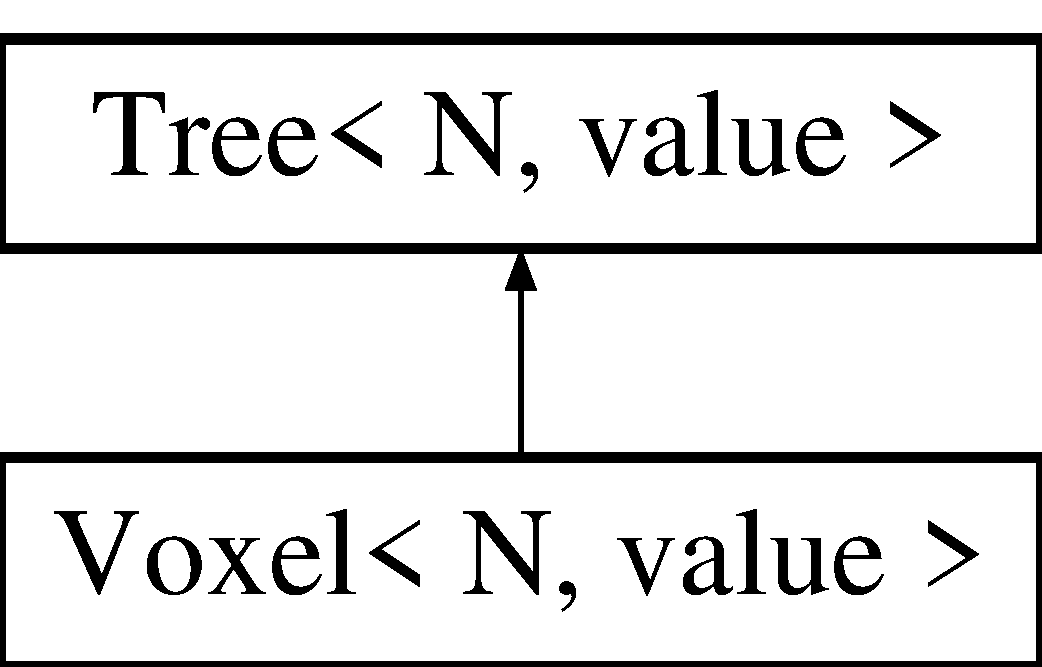
\includegraphics[height=2.000000cm]{classVoxel}
\end{center}
\end{figure}
\subsection*{Public Member Functions}
\begin{DoxyCompactItemize}
\item 
\mbox{\hyperlink{classVoxel_a2de5f4a796b6232664726a75cc727873}{Voxel}} (\mbox{\hyperlink{definitions_8h_aedc0ad84d1e764530814f57ad931d02a}{real}} $\ast$length, \mbox{\hyperlink{definitions_8h_aedc0ad84d1e764530814f57ad931d02a}{real}} $\ast$coords)
\item 
void \mbox{\hyperlink{classVoxel_af363467297ff56e7f67c8b8e433fba04}{set\+Level}} (\mbox{\hyperlink{definitions_8h_a69aa29b598b851b0640aa225a9e5d61d}{uint}} $\ast$l)
\item 
void \mbox{\hyperlink{classVoxel_acf4017ddfe4ecfb418cd4c8828eec71d}{generate\+Search\+Tree}} (\mbox{\hyperlink{definitions_8h_aedc0ad84d1e764530814f57ad931d02a}{real}} $\ast$geom\+\_\+xyz, \mbox{\hyperlink{definitions_8h_a69aa29b598b851b0640aa225a9e5d61d}{uint}} n)
\item 
void \mbox{\hyperlink{classVoxel_a97154e50e16297f2f9e81cac91271aee}{distribute\+Geom\+To\+Leaves}} (\mbox{\hyperlink{definitions_8h_aedc0ad84d1e764530814f57ad931d02a}{real}} $\ast$geom\+\_\+xyz, \mbox{\hyperlink{definitions_8h_a69aa29b598b851b0640aa225a9e5d61d}{uint}} n)
\item 
\mbox{\hyperlink{definitions_8h_a69aa29b598b851b0640aa225a9e5d61d}{uint}} \mbox{\hyperlink{classVoxel_a3f219470ab58fc5da5431566fd093378}{check\+Sibling\+Status}} (\mbox{\hyperlink{definitions_8h_af8682350bd8bb38ee9023f7a0a310add}{morton}}$<$ N $>$ key, \mbox{\hyperlink{definitions_8h_af8682350bd8bb38ee9023f7a0a310add}{morton}}$<$ N $>$ $\ast$sibkey)
\item 
void \mbox{\hyperlink{classVoxel_ad34c50e8ed627e20dba6188a1c074854}{derefine\+Geom\+Tree}} ()
\item 
bool \mbox{\hyperlink{classVoxel_af2e7050a3c6d74c62c929d6b08f123b3}{Is\+Inside\+Segment}} (\mbox{\hyperlink{definitions_8h_af8682350bd8bb38ee9023f7a0a310add}{morton}}$<$ N $>$ key, \mbox{\hyperlink{definitions_8h_aedc0ad84d1e764530814f57ad931d02a}{real}} $\ast$xyz)
\item 
\mbox{\hyperlink{classVoxel_a4e96d3d825885a1728f478bba74cd3c9}{$\sim$\+Voxel}} ()
\end{DoxyCompactItemize}
\subsection*{Private Attributes}
\begin{DoxyCompactItemize}
\item 
\mbox{\hyperlink{definitions_8h_a69aa29b598b851b0640aa225a9e5d61d}{uint}} \mbox{\hyperlink{classVoxel_addc02aaaef2f93ffcae1ded7a2184518}{maxlevel}}
\item 
\mbox{\hyperlink{definitions_8h_a69aa29b598b851b0640aa225a9e5d61d}{uint}} \mbox{\hyperlink{classVoxel_addfa7b07b7173c6727fd8cf0c38c61d8}{num\+Max}}
\item 
\mbox{\hyperlink{definitions_8h_acf2396ef4de9eb8a6324b9f1a624ea85}{bitmap}}$<$ N, value $>$ \mbox{\hyperlink{classVoxel_a3d53e01604350cc00c9bef098c7e23e5}{mesh}}
\item 
\mbox{\hyperlink{definitions_8h_a55821d7929f3f16aaf1466129c209492}{bitvector}}$<$ N $>$ \mbox{\hyperlink{classVoxel_a4e8a1661e9468250e10aa861d61f861e}{lookup}}
\end{DoxyCompactItemize}
\subsection*{Friends}
\begin{DoxyCompactItemize}
\item 
{\footnotesize template$<$size\+\_\+t N1, typename value1 $>$ }\\class \mbox{\hyperlink{classVoxel_a7f84a23096bb6840efa341b4cde72d9d}{Hdf5\+XmfV}}
\end{DoxyCompactItemize}
\subsection*{Additional Inherited Members}


\subsection{Detailed Description}
\subsubsection*{template$<$size\+\_\+t N, typename value$>$\newline
class Voxel$<$ N, value $>$}

This Class Generates an unbalancerd \mbox{\hyperlink{classVoxel}{Voxel}} to improve search by geometry partitioning. 

\subsection{Constructor \& Destructor Documentation}
\mbox{\Hypertarget{classVoxel_a2de5f4a796b6232664726a75cc727873}\label{classVoxel_a2de5f4a796b6232664726a75cc727873}} 
\index{Voxel@{Voxel}!Voxel@{Voxel}}
\index{Voxel@{Voxel}!Voxel@{Voxel}}
\subsubsection{\texorpdfstring{Voxel()}{Voxel()}}
{\footnotesize\ttfamily template$<$size\+\_\+t N, typename value$>$ \\
\mbox{\hyperlink{classVoxel}{Voxel}}$<$ N, value $>$\+::\mbox{\hyperlink{classVoxel}{Voxel}} (\begin{DoxyParamCaption}\item[{\mbox{\hyperlink{definitions_8h_aedc0ad84d1e764530814f57ad931d02a}{real}} $\ast$}]{length,  }\item[{\mbox{\hyperlink{definitions_8h_aedc0ad84d1e764530814f57ad931d02a}{real}} $\ast$}]{coords }\end{DoxyParamCaption})\hspace{0.3cm}{\ttfamily [inline]}}

\mbox{\Hypertarget{classVoxel_a4e96d3d825885a1728f478bba74cd3c9}\label{classVoxel_a4e96d3d825885a1728f478bba74cd3c9}} 
\index{Voxel@{Voxel}!````~Voxel@{$\sim$\+Voxel}}
\index{````~Voxel@{$\sim$\+Voxel}!Voxel@{Voxel}}
\subsubsection{\texorpdfstring{$\sim$\+Voxel()}{~Voxel()}}
{\footnotesize\ttfamily template$<$size\+\_\+t N, typename value $>$ \\
\mbox{\hyperlink{classVoxel}{Voxel}}$<$ N, value $>$\+::$\sim$\mbox{\hyperlink{classVoxel}{Voxel}} (\begin{DoxyParamCaption}{ }\end{DoxyParamCaption})}

Destructor of this class 

\subsection{Member Function Documentation}
\mbox{\Hypertarget{classVoxel_a3f219470ab58fc5da5431566fd093378}\label{classVoxel_a3f219470ab58fc5da5431566fd093378}} 
\index{Voxel@{Voxel}!check\+Sibling\+Status@{check\+Sibling\+Status}}
\index{check\+Sibling\+Status@{check\+Sibling\+Status}!Voxel@{Voxel}}
\subsubsection{\texorpdfstring{check\+Sibling\+Status()}{checkSiblingStatus()}}
{\footnotesize\ttfamily template$<$size\+\_\+t N, typename value $>$ \\
\mbox{\hyperlink{definitions_8h_a69aa29b598b851b0640aa225a9e5d61d}{uint}} \mbox{\hyperlink{classVoxel}{Voxel}}$<$ N, value $>$\+::check\+Sibling\+Status (\begin{DoxyParamCaption}\item[{\mbox{\hyperlink{definitions_8h_af8682350bd8bb38ee9023f7a0a310add}{morton}}$<$ N $>$}]{key,  }\item[{\mbox{\hyperlink{definitions_8h_af8682350bd8bb38ee9023f7a0a310add}{morton}}$<$ N $>$ $\ast$}]{sibkey }\end{DoxyParamCaption})}


\begin{DoxyParams}{Parameters}
{\em sibkey} & checks to see if siblings include any points and whether they have the same level \\
\hline
\end{DoxyParams}
\mbox{\Hypertarget{classVoxel_ad34c50e8ed627e20dba6188a1c074854}\label{classVoxel_ad34c50e8ed627e20dba6188a1c074854}} 
\index{Voxel@{Voxel}!derefine\+Geom\+Tree@{derefine\+Geom\+Tree}}
\index{derefine\+Geom\+Tree@{derefine\+Geom\+Tree}!Voxel@{Voxel}}
\subsubsection{\texorpdfstring{derefine\+Geom\+Tree()}{derefineGeomTree()}}
{\footnotesize\ttfamily template$<$size\+\_\+t N, typename value $>$ \\
void \mbox{\hyperlink{classVoxel}{Voxel}}$<$ N, value $>$\+::derefine\+Geom\+Tree (\begin{DoxyParamCaption}{ }\end{DoxyParamCaption})}

checks to see if siblings include any points and whether they have the same level derefines the tree based on geometry \mbox{\Hypertarget{classVoxel_a97154e50e16297f2f9e81cac91271aee}\label{classVoxel_a97154e50e16297f2f9e81cac91271aee}} 
\index{Voxel@{Voxel}!distribute\+Geom\+To\+Leaves@{distribute\+Geom\+To\+Leaves}}
\index{distribute\+Geom\+To\+Leaves@{distribute\+Geom\+To\+Leaves}!Voxel@{Voxel}}
\subsubsection{\texorpdfstring{distribute\+Geom\+To\+Leaves()}{distributeGeomToLeaves()}}
{\footnotesize\ttfamily template$<$size\+\_\+t N, typename value $>$ \\
void \mbox{\hyperlink{classVoxel}{Voxel}}$<$ N, value $>$\+::distribute\+Geom\+To\+Leaves (\begin{DoxyParamCaption}\item[{\mbox{\hyperlink{definitions_8h_aedc0ad84d1e764530814f57ad931d02a}{real}} $\ast$}]{geom\+\_\+xyz,  }\item[{\mbox{\hyperlink{definitions_8h_a69aa29b598b851b0640aa225a9e5d61d}{uint}}}]{n }\end{DoxyParamCaption})}

distributes geometry to different cells (leaves) \mbox{\Hypertarget{classVoxel_acf4017ddfe4ecfb418cd4c8828eec71d}\label{classVoxel_acf4017ddfe4ecfb418cd4c8828eec71d}} 
\index{Voxel@{Voxel}!generate\+Search\+Tree@{generate\+Search\+Tree}}
\index{generate\+Search\+Tree@{generate\+Search\+Tree}!Voxel@{Voxel}}
\subsubsection{\texorpdfstring{generate\+Search\+Tree()}{generateSearchTree()}}
{\footnotesize\ttfamily template$<$size\+\_\+t N, typename value $>$ \\
void \mbox{\hyperlink{classVoxel}{Voxel}}$<$ N, value $>$\+::generate\+Search\+Tree (\begin{DoxyParamCaption}\item[{\mbox{\hyperlink{definitions_8h_aedc0ad84d1e764530814f57ad931d02a}{real}} $\ast$}]{geom\+\_\+xyz,  }\item[{\mbox{\hyperlink{definitions_8h_a69aa29b598b851b0640aa225a9e5d61d}{uint}}}]{n }\end{DoxyParamCaption})}

generates an initial tree \mbox{\Hypertarget{classVoxel_af2e7050a3c6d74c62c929d6b08f123b3}\label{classVoxel_af2e7050a3c6d74c62c929d6b08f123b3}} 
\index{Voxel@{Voxel}!Is\+Inside\+Segment@{Is\+Inside\+Segment}}
\index{Is\+Inside\+Segment@{Is\+Inside\+Segment}!Voxel@{Voxel}}
\subsubsection{\texorpdfstring{Is\+Inside\+Segment()}{IsInsideSegment()}}
{\footnotesize\ttfamily template$<$size\+\_\+t N, typename value $>$ \\
bool \mbox{\hyperlink{classVoxel}{Voxel}}$<$ N, value $>$\+::Is\+Inside\+Segment (\begin{DoxyParamCaption}\item[{\mbox{\hyperlink{definitions_8h_af8682350bd8bb38ee9023f7a0a310add}{morton}}$<$ N $>$}]{key,  }\item[{\mbox{\hyperlink{definitions_8h_aedc0ad84d1e764530814f57ad931d02a}{real}} $\ast$}]{xyz }\end{DoxyParamCaption})}

\mbox{\Hypertarget{classVoxel_af363467297ff56e7f67c8b8e433fba04}\label{classVoxel_af363467297ff56e7f67c8b8e433fba04}} 
\index{Voxel@{Voxel}!set\+Level@{set\+Level}}
\index{set\+Level@{set\+Level}!Voxel@{Voxel}}
\subsubsection{\texorpdfstring{set\+Level()}{setLevel()}}
{\footnotesize\ttfamily template$<$size\+\_\+t N, typename value $>$ \\
void \mbox{\hyperlink{classVoxel}{Voxel}}$<$ N, value $>$\+::set\+Level (\begin{DoxyParamCaption}\item[{\mbox{\hyperlink{definitions_8h_a69aa29b598b851b0640aa225a9e5d61d}{uint}} $\ast$}]{l }\end{DoxyParamCaption})}

constructor sets the maximum level for refinement 

\subsection{Friends And Related Function Documentation}
\mbox{\Hypertarget{classVoxel_a7f84a23096bb6840efa341b4cde72d9d}\label{classVoxel_a7f84a23096bb6840efa341b4cde72d9d}} 
\index{Voxel@{Voxel}!Hdf5\+XmfV@{Hdf5\+XmfV}}
\index{Hdf5\+XmfV@{Hdf5\+XmfV}!Voxel@{Voxel}}
\subsubsection{\texorpdfstring{Hdf5\+XmfV}{Hdf5XmfV}}
{\footnotesize\ttfamily template$<$size\+\_\+t N, typename value$>$ \\
template$<$size\+\_\+t N1, typename value1 $>$ \\
friend class Hdf5\+XmfV\hspace{0.3cm}{\ttfamily [friend]}}

this is a friend class to write out in hdf5 format 

\subsection{Member Data Documentation}
\mbox{\Hypertarget{classVoxel_a4e8a1661e9468250e10aa861d61f861e}\label{classVoxel_a4e8a1661e9468250e10aa861d61f861e}} 
\index{Voxel@{Voxel}!lookup@{lookup}}
\index{lookup@{lookup}!Voxel@{Voxel}}
\subsubsection{\texorpdfstring{lookup}{lookup}}
{\footnotesize\ttfamily template$<$size\+\_\+t N, typename value$>$ \\
\mbox{\hyperlink{definitions_8h_a55821d7929f3f16aaf1466129c209492}{bitvector}}$<$N$>$ \mbox{\hyperlink{classVoxel}{Voxel}}$<$ N, value $>$\+::lookup\hspace{0.3cm}{\ttfamily [private]}}

\mbox{\Hypertarget{classVoxel_addc02aaaef2f93ffcae1ded7a2184518}\label{classVoxel_addc02aaaef2f93ffcae1ded7a2184518}} 
\index{Voxel@{Voxel}!maxlevel@{maxlevel}}
\index{maxlevel@{maxlevel}!Voxel@{Voxel}}
\subsubsection{\texorpdfstring{maxlevel}{maxlevel}}
{\footnotesize\ttfamily template$<$size\+\_\+t N, typename value$>$ \\
\mbox{\hyperlink{definitions_8h_a69aa29b598b851b0640aa225a9e5d61d}{uint}} \mbox{\hyperlink{classVoxel}{Voxel}}$<$ N, value $>$\+::maxlevel\hspace{0.3cm}{\ttfamily [private]}}

maximum level of refinement \mbox{\Hypertarget{classVoxel_a3d53e01604350cc00c9bef098c7e23e5}\label{classVoxel_a3d53e01604350cc00c9bef098c7e23e5}} 
\index{Voxel@{Voxel}!mesh@{mesh}}
\index{mesh@{mesh}!Voxel@{Voxel}}
\subsubsection{\texorpdfstring{mesh}{mesh}}
{\footnotesize\ttfamily template$<$size\+\_\+t N, typename value$>$ \\
\mbox{\hyperlink{definitions_8h_acf2396ef4de9eb8a6324b9f1a624ea85}{bitmap}}$<$N, value$>$ \mbox{\hyperlink{classVoxel}{Voxel}}$<$ N, value $>$\+::mesh\hspace{0.3cm}{\ttfamily [private]}}

\mbox{\Hypertarget{classVoxel_addfa7b07b7173c6727fd8cf0c38c61d8}\label{classVoxel_addfa7b07b7173c6727fd8cf0c38c61d8}} 
\index{Voxel@{Voxel}!num\+Max@{num\+Max}}
\index{num\+Max@{num\+Max}!Voxel@{Voxel}}
\subsubsection{\texorpdfstring{num\+Max}{numMax}}
{\footnotesize\ttfamily template$<$size\+\_\+t N, typename value$>$ \\
\mbox{\hyperlink{definitions_8h_a69aa29b598b851b0640aa225a9e5d61d}{uint}} \mbox{\hyperlink{classVoxel}{Voxel}}$<$ N, value $>$\+::num\+Max\hspace{0.3cm}{\ttfamily [private]}}

number of elements having the highest level 

The documentation for this class was generated from the following files\+:\begin{DoxyCompactItemize}
\item 
/ihome/isenocak/jaber/\+Morton\+\_\+\+Parallel\+\_\+v0/test/\+Morton\+\_\+\+Parallel\+\_\+v0/src/include/\mbox{\hyperlink{tree_8h}{tree.\+h}}\item 
/ihome/isenocak/jaber/\+Morton\+\_\+\+Parallel\+\_\+v0/test/\+Morton\+\_\+\+Parallel\+\_\+v0/src/\mbox{\hyperlink{voxel_8cpp}{voxel.\+cpp}}\end{DoxyCompactItemize}

\hypertarget{structZoltan__Out}{}\section{Zoltan\+\_\+\+Out Struct Reference}
\label{structZoltan__Out}\index{Zoltan\+\_\+\+Out@{Zoltan\+\_\+\+Out}}


This structure is an interface to store the output from Zoltan.  




{\ttfamily \#include $<$typedefs.\+h$>$}

\subsection*{Public Attributes}
\begin{DoxyCompactItemize}
\item 
int \mbox{\hyperlink{structZoltan__Out_a4a16fd4f8cc9d38d47810055e8b7b97b}{changes}}
\item 
int \mbox{\hyperlink{structZoltan__Out_a9ec8c391f2218e927b8e9f31fd49ee72}{num\+Gid\+Entries}}
\item 
int \mbox{\hyperlink{structZoltan__Out_a1de4e895402c6a3ceb3735c70ec88c23}{num\+Lid\+Entries}}
\item 
int \mbox{\hyperlink{structZoltan__Out_a3ec6846e956ee5337cb94c69b8bef4ce}{num\+Import}}
\item 
int \mbox{\hyperlink{structZoltan__Out_ae3c782bd4b01650d2ec6f970ec0df24b}{num\+Export}}
\item 
unsigned int $\ast$ \mbox{\hyperlink{structZoltan__Out_a2c70ebf8c353ba745560459779090703}{import\+Global\+Gids}}
\item 
unsigned int $\ast$ \mbox{\hyperlink{structZoltan__Out_aaabd5873a7bd360c3d02499c13455bc2}{import\+Local\+Gids}}
\item 
unsigned int $\ast$ \mbox{\hyperlink{structZoltan__Out_a41a465f7840cecafd959c81c56d57e9d}{export\+Global\+Gids}}
\item 
unsigned int $\ast$ \mbox{\hyperlink{structZoltan__Out_a7a5c47580bc0a77cd51f0179b0b9d92b}{export\+Local\+Gids}}
\item 
int $\ast$ \mbox{\hyperlink{structZoltan__Out_a6421b3c6ccec98151928ef6461be97e2}{import\+Procs}}
\item 
int $\ast$ \mbox{\hyperlink{structZoltan__Out_ac8fcf42b3806fe7b52f5455d67814098}{import\+To\+Part}}
\item 
int $\ast$ \mbox{\hyperlink{structZoltan__Out_a934d6621722a687a3d8b7bf43c259816}{export\+Procs}}
\item 
int $\ast$ \mbox{\hyperlink{structZoltan__Out_ab2a81da9a9d6ac69b69f5db89e97c6bf}{export\+To\+Part}}
\item 
int $\ast$ \mbox{\hyperlink{structZoltan__Out_addc3ad3c22e6fb8e7073de71425d4ead}{parts}}
\end{DoxyCompactItemize}


\subsection{Detailed Description}
This structure is an interface to store the output from Zoltan. 

\subsection{Member Data Documentation}
\mbox{\Hypertarget{structZoltan__Out_a4a16fd4f8cc9d38d47810055e8b7b97b}\label{structZoltan__Out_a4a16fd4f8cc9d38d47810055e8b7b97b}} 
\index{Zoltan\+\_\+\+Out@{Zoltan\+\_\+\+Out}!changes@{changes}}
\index{changes@{changes}!Zoltan\+\_\+\+Out@{Zoltan\+\_\+\+Out}}
\subsubsection{\texorpdfstring{changes}{changes}}
{\footnotesize\ttfamily int Zoltan\+\_\+\+Out\+::changes}

\mbox{\Hypertarget{structZoltan__Out_a41a465f7840cecafd959c81c56d57e9d}\label{structZoltan__Out_a41a465f7840cecafd959c81c56d57e9d}} 
\index{Zoltan\+\_\+\+Out@{Zoltan\+\_\+\+Out}!export\+Global\+Gids@{export\+Global\+Gids}}
\index{export\+Global\+Gids@{export\+Global\+Gids}!Zoltan\+\_\+\+Out@{Zoltan\+\_\+\+Out}}
\subsubsection{\texorpdfstring{export\+Global\+Gids}{exportGlobalGids}}
{\footnotesize\ttfamily unsigned int$\ast$ Zoltan\+\_\+\+Out\+::export\+Global\+Gids}

\mbox{\Hypertarget{structZoltan__Out_a7a5c47580bc0a77cd51f0179b0b9d92b}\label{structZoltan__Out_a7a5c47580bc0a77cd51f0179b0b9d92b}} 
\index{Zoltan\+\_\+\+Out@{Zoltan\+\_\+\+Out}!export\+Local\+Gids@{export\+Local\+Gids}}
\index{export\+Local\+Gids@{export\+Local\+Gids}!Zoltan\+\_\+\+Out@{Zoltan\+\_\+\+Out}}
\subsubsection{\texorpdfstring{export\+Local\+Gids}{exportLocalGids}}
{\footnotesize\ttfamily unsigned int$\ast$ Zoltan\+\_\+\+Out\+::export\+Local\+Gids}

\mbox{\Hypertarget{structZoltan__Out_a934d6621722a687a3d8b7bf43c259816}\label{structZoltan__Out_a934d6621722a687a3d8b7bf43c259816}} 
\index{Zoltan\+\_\+\+Out@{Zoltan\+\_\+\+Out}!export\+Procs@{export\+Procs}}
\index{export\+Procs@{export\+Procs}!Zoltan\+\_\+\+Out@{Zoltan\+\_\+\+Out}}
\subsubsection{\texorpdfstring{export\+Procs}{exportProcs}}
{\footnotesize\ttfamily int$\ast$ Zoltan\+\_\+\+Out\+::export\+Procs}

\mbox{\Hypertarget{structZoltan__Out_ab2a81da9a9d6ac69b69f5db89e97c6bf}\label{structZoltan__Out_ab2a81da9a9d6ac69b69f5db89e97c6bf}} 
\index{Zoltan\+\_\+\+Out@{Zoltan\+\_\+\+Out}!export\+To\+Part@{export\+To\+Part}}
\index{export\+To\+Part@{export\+To\+Part}!Zoltan\+\_\+\+Out@{Zoltan\+\_\+\+Out}}
\subsubsection{\texorpdfstring{export\+To\+Part}{exportToPart}}
{\footnotesize\ttfamily int$\ast$ Zoltan\+\_\+\+Out\+::export\+To\+Part}

\mbox{\Hypertarget{structZoltan__Out_a2c70ebf8c353ba745560459779090703}\label{structZoltan__Out_a2c70ebf8c353ba745560459779090703}} 
\index{Zoltan\+\_\+\+Out@{Zoltan\+\_\+\+Out}!import\+Global\+Gids@{import\+Global\+Gids}}
\index{import\+Global\+Gids@{import\+Global\+Gids}!Zoltan\+\_\+\+Out@{Zoltan\+\_\+\+Out}}
\subsubsection{\texorpdfstring{import\+Global\+Gids}{importGlobalGids}}
{\footnotesize\ttfamily unsigned int$\ast$ Zoltan\+\_\+\+Out\+::import\+Global\+Gids}

\mbox{\Hypertarget{structZoltan__Out_aaabd5873a7bd360c3d02499c13455bc2}\label{structZoltan__Out_aaabd5873a7bd360c3d02499c13455bc2}} 
\index{Zoltan\+\_\+\+Out@{Zoltan\+\_\+\+Out}!import\+Local\+Gids@{import\+Local\+Gids}}
\index{import\+Local\+Gids@{import\+Local\+Gids}!Zoltan\+\_\+\+Out@{Zoltan\+\_\+\+Out}}
\subsubsection{\texorpdfstring{import\+Local\+Gids}{importLocalGids}}
{\footnotesize\ttfamily unsigned int$\ast$ Zoltan\+\_\+\+Out\+::import\+Local\+Gids}

\mbox{\Hypertarget{structZoltan__Out_a6421b3c6ccec98151928ef6461be97e2}\label{structZoltan__Out_a6421b3c6ccec98151928ef6461be97e2}} 
\index{Zoltan\+\_\+\+Out@{Zoltan\+\_\+\+Out}!import\+Procs@{import\+Procs}}
\index{import\+Procs@{import\+Procs}!Zoltan\+\_\+\+Out@{Zoltan\+\_\+\+Out}}
\subsubsection{\texorpdfstring{import\+Procs}{importProcs}}
{\footnotesize\ttfamily int$\ast$ Zoltan\+\_\+\+Out\+::import\+Procs}

\mbox{\Hypertarget{structZoltan__Out_ac8fcf42b3806fe7b52f5455d67814098}\label{structZoltan__Out_ac8fcf42b3806fe7b52f5455d67814098}} 
\index{Zoltan\+\_\+\+Out@{Zoltan\+\_\+\+Out}!import\+To\+Part@{import\+To\+Part}}
\index{import\+To\+Part@{import\+To\+Part}!Zoltan\+\_\+\+Out@{Zoltan\+\_\+\+Out}}
\subsubsection{\texorpdfstring{import\+To\+Part}{importToPart}}
{\footnotesize\ttfamily int$\ast$ Zoltan\+\_\+\+Out\+::import\+To\+Part}

\mbox{\Hypertarget{structZoltan__Out_ae3c782bd4b01650d2ec6f970ec0df24b}\label{structZoltan__Out_ae3c782bd4b01650d2ec6f970ec0df24b}} 
\index{Zoltan\+\_\+\+Out@{Zoltan\+\_\+\+Out}!num\+Export@{num\+Export}}
\index{num\+Export@{num\+Export}!Zoltan\+\_\+\+Out@{Zoltan\+\_\+\+Out}}
\subsubsection{\texorpdfstring{num\+Export}{numExport}}
{\footnotesize\ttfamily int Zoltan\+\_\+\+Out\+::num\+Export}

\mbox{\Hypertarget{structZoltan__Out_a9ec8c391f2218e927b8e9f31fd49ee72}\label{structZoltan__Out_a9ec8c391f2218e927b8e9f31fd49ee72}} 
\index{Zoltan\+\_\+\+Out@{Zoltan\+\_\+\+Out}!num\+Gid\+Entries@{num\+Gid\+Entries}}
\index{num\+Gid\+Entries@{num\+Gid\+Entries}!Zoltan\+\_\+\+Out@{Zoltan\+\_\+\+Out}}
\subsubsection{\texorpdfstring{num\+Gid\+Entries}{numGidEntries}}
{\footnotesize\ttfamily int Zoltan\+\_\+\+Out\+::num\+Gid\+Entries}

\mbox{\Hypertarget{structZoltan__Out_a3ec6846e956ee5337cb94c69b8bef4ce}\label{structZoltan__Out_a3ec6846e956ee5337cb94c69b8bef4ce}} 
\index{Zoltan\+\_\+\+Out@{Zoltan\+\_\+\+Out}!num\+Import@{num\+Import}}
\index{num\+Import@{num\+Import}!Zoltan\+\_\+\+Out@{Zoltan\+\_\+\+Out}}
\subsubsection{\texorpdfstring{num\+Import}{numImport}}
{\footnotesize\ttfamily int Zoltan\+\_\+\+Out\+::num\+Import}

\mbox{\Hypertarget{structZoltan__Out_a1de4e895402c6a3ceb3735c70ec88c23}\label{structZoltan__Out_a1de4e895402c6a3ceb3735c70ec88c23}} 
\index{Zoltan\+\_\+\+Out@{Zoltan\+\_\+\+Out}!num\+Lid\+Entries@{num\+Lid\+Entries}}
\index{num\+Lid\+Entries@{num\+Lid\+Entries}!Zoltan\+\_\+\+Out@{Zoltan\+\_\+\+Out}}
\subsubsection{\texorpdfstring{num\+Lid\+Entries}{numLidEntries}}
{\footnotesize\ttfamily int Zoltan\+\_\+\+Out\+::num\+Lid\+Entries}

\mbox{\Hypertarget{structZoltan__Out_addc3ad3c22e6fb8e7073de71425d4ead}\label{structZoltan__Out_addc3ad3c22e6fb8e7073de71425d4ead}} 
\index{Zoltan\+\_\+\+Out@{Zoltan\+\_\+\+Out}!parts@{parts}}
\index{parts@{parts}!Zoltan\+\_\+\+Out@{Zoltan\+\_\+\+Out}}
\subsubsection{\texorpdfstring{parts}{parts}}
{\footnotesize\ttfamily int$\ast$ Zoltan\+\_\+\+Out\+::parts}



The documentation for this struct was generated from the following file\+:\begin{DoxyCompactItemize}
\item 
/ihome/isenocak/jaber/\+Morton\+\_\+\+Parallel\+\_\+v0/test/\+Morton\+\_\+\+Parallel\+\_\+v0/src/include/\mbox{\hyperlink{typedefs_8h}{typedefs.\+h}}\end{DoxyCompactItemize}

\chapter{File Documentation}
\hypertarget{communicate_8cpp}{}\section{/ihome/isenocak/jaber/\+Morton\+\_\+\+Parallel\+\_\+v0/test/\+Morton\+\_\+\+Parallel\+\_\+v0/src/communicate.cpp File Reference}
\label{communicate_8cpp}\index{/ihome/isenocak/jaber/\+Morton\+\_\+\+Parallel\+\_\+v0/test/\+Morton\+\_\+\+Parallel\+\_\+v0/src/communicate.\+cpp@{/ihome/isenocak/jaber/\+Morton\+\_\+\+Parallel\+\_\+v0/test/\+Morton\+\_\+\+Parallel\+\_\+v0/src/communicate.\+cpp}}
{\ttfamily \#include \char`\"{}communicate.\+h\char`\"{}}\newline
{\ttfamily \#include \char`\"{}datatype.\+h\char`\"{}}\newline
\subsection*{Functions}
\begin{DoxyCompactItemize}
\item 
static M\+P\+I\+\_\+\+Datatype \mbox{\hyperlink{communicate_8cpp_a214470942d424bf40235334f7b12033a}{Convert\+Type}} (\mbox{\hyperlink{namespaceAbstraction_a4cb76335aa0f291a9c5e3243653142b6}{Abstraction\+::\+Data\+Type}} type)
\end{DoxyCompactItemize}


\subsection{Function Documentation}
\mbox{\Hypertarget{communicate_8cpp_a214470942d424bf40235334f7b12033a}\label{communicate_8cpp_a214470942d424bf40235334f7b12033a}} 
\index{communicate.\+cpp@{communicate.\+cpp}!Convert\+Type@{Convert\+Type}}
\index{Convert\+Type@{Convert\+Type}!communicate.\+cpp@{communicate.\+cpp}}
\subsubsection{\texorpdfstring{Convert\+Type()}{ConvertType()}}
{\footnotesize\ttfamily static M\+P\+I\+\_\+\+Datatype Convert\+Type (\begin{DoxyParamCaption}\item[{\mbox{\hyperlink{namespaceAbstraction_a4cb76335aa0f291a9c5e3243653142b6}{Abstraction\+::\+Data\+Type}}}]{type }\end{DoxyParamCaption})\hspace{0.3cm}{\ttfamily [static]}}

communicate class member functions \mbox{\hyperlink{classCommPoint2Point}{Comm\+Point2\+Point}} This Class is a wrapper around M\+PI functions used in this project

Templating the \char`\"{}\+Intrinsic Type Conversion Using Template Specialization\char`\"{} message tag and mpi\+\_\+communicators are assigned by default if user doesnt assign them default tag is 0 and default Communicator is M\+P\+I\+\_\+\+C\+O\+M\+M\+\_\+\+W\+O\+R\+LD 
\hypertarget{full__tree_8cpp}{}\section{/ihome/isenocak/jaber/\+Morton\+\_\+\+Parallel\+\_\+v0/test/\+Morton\+\_\+\+Parallel\+\_\+v0/src/full\+\_\+tree.cpp File Reference}
\label{full__tree_8cpp}\index{/ihome/isenocak/jaber/\+Morton\+\_\+\+Parallel\+\_\+v0/test/\+Morton\+\_\+\+Parallel\+\_\+v0/src/full\+\_\+tree.\+cpp@{/ihome/isenocak/jaber/\+Morton\+\_\+\+Parallel\+\_\+v0/test/\+Morton\+\_\+\+Parallel\+\_\+v0/src/full\+\_\+tree.\+cpp}}
{\ttfamily \#include \char`\"{}tree.\+h\char`\"{}}\newline
{\ttfamily \#include \char`\"{}definitions.\+h\char`\"{}}\newline
{\ttfamily \#include \char`\"{}typedefs.\+h\char`\"{}}\newline

\hypertarget{geomSTL_8cpp}{}\section{/ihome/isenocak/jaber/\+Morton\+\_\+\+Parallel\+\_\+v0/test/\+Morton\+\_\+\+Parallel\+\_\+v0/src/geom\+S\+TL.cpp File Reference}
\label{geomSTL_8cpp}\index{/ihome/isenocak/jaber/\+Morton\+\_\+\+Parallel\+\_\+v0/test/\+Morton\+\_\+\+Parallel\+\_\+v0/src/geom\+S\+T\+L.\+cpp@{/ihome/isenocak/jaber/\+Morton\+\_\+\+Parallel\+\_\+v0/test/\+Morton\+\_\+\+Parallel\+\_\+v0/src/geom\+S\+T\+L.\+cpp}}
{\ttfamily \#include \char`\"{}geom\+S\+T\+L.\+h\char`\"{}}\newline
{\ttfamily \#include \char`\"{}definitions.\+h\char`\"{}}\newline
\subsection*{Macros}
\begin{DoxyCompactItemize}
\item 
\#define \mbox{\hyperlink{geomSTL_8cpp_aea8c2e7a86e2819ce737586c4db0901f}{M\+Y\+S\+C\+A\+LE}}~0.\+5
\end{DoxyCompactItemize}


\subsection{Macro Definition Documentation}
\mbox{\Hypertarget{geomSTL_8cpp_aea8c2e7a86e2819ce737586c4db0901f}\label{geomSTL_8cpp_aea8c2e7a86e2819ce737586c4db0901f}} 
\index{geom\+S\+T\+L.\+cpp@{geom\+S\+T\+L.\+cpp}!M\+Y\+S\+C\+A\+LE@{M\+Y\+S\+C\+A\+LE}}
\index{M\+Y\+S\+C\+A\+LE@{M\+Y\+S\+C\+A\+LE}!geom\+S\+T\+L.\+cpp@{geom\+S\+T\+L.\+cpp}}
\subsubsection{\texorpdfstring{M\+Y\+S\+C\+A\+LE}{MYSCALE}}
{\footnotesize\ttfamily \#define M\+Y\+S\+C\+A\+LE~0.\+5}


\hypertarget{communicate_8h}{}\section{/ihome/isenocak/jaber/\+Morton\+\_\+\+Parallel\+\_\+v0/test/\+Morton\+\_\+\+Parallel\+\_\+v0/src/include/communicate.h File Reference}
\label{communicate_8h}\index{/ihome/isenocak/jaber/\+Morton\+\_\+\+Parallel\+\_\+v0/test/\+Morton\+\_\+\+Parallel\+\_\+v0/src/include/communicate.\+h@{/ihome/isenocak/jaber/\+Morton\+\_\+\+Parallel\+\_\+v0/test/\+Morton\+\_\+\+Parallel\+\_\+v0/src/include/communicate.\+h}}
{\ttfamily \#include \char`\"{}definitions.\+h\char`\"{}}\newline
\subsection*{Classes}
\begin{DoxyCompactItemize}
\item 
struct \mbox{\hyperlink{structMpiCom}{Mpi\+Com}}
\begin{DoxyCompactList}\small\item\em class for embedding data related to the communicator \end{DoxyCompactList}\item 
struct \mbox{\hyperlink{structMessage}{Message}}
\begin{DoxyCompactList}\small\item\em struct that embeds data related to the message and envelope \end{DoxyCompactList}\item 
class \mbox{\hyperlink{classCommPoint2Point}{Comm\+Point2\+Point$<$ Type $>$}}
\begin{DoxyCompactList}\small\item\em A template wrapper around M\+PI functions for point to point communication. \end{DoxyCompactList}\item 
class \mbox{\hyperlink{classCommCollective}{Comm\+Collective$<$ Type $>$}}
\begin{DoxyCompactList}\small\item\em is a template wrapper around M\+PI functions for collective communicatios \end{DoxyCompactList}\end{DoxyCompactItemize}

\hypertarget{datatype_8h}{}\section{/ihome/isenocak/jaber/\+Morton\+\_\+\+Parallel\+\_\+v0/test/\+Morton\+\_\+\+Parallel\+\_\+v0/src/include/datatype.h File Reference}
\label{datatype_8h}\index{/ihome/isenocak/jaber/\+Morton\+\_\+\+Parallel\+\_\+v0/test/\+Morton\+\_\+\+Parallel\+\_\+v0/src/include/datatype.\+h@{/ihome/isenocak/jaber/\+Morton\+\_\+\+Parallel\+\_\+v0/test/\+Morton\+\_\+\+Parallel\+\_\+v0/src/include/datatype.\+h}}
{\ttfamily \#include \char`\"{}definitions.\+h\char`\"{}}\newline
\subsection*{Namespaces}
\begin{DoxyCompactItemize}
\item 
 \mbox{\hyperlink{namespaceAbstraction}{Abstraction}}
\end{DoxyCompactItemize}
\subsection*{Enumerations}
\begin{DoxyCompactItemize}
\item 
enum \mbox{\hyperlink{namespaceAbstraction_a4cb76335aa0f291a9c5e3243653142b6}{Abstraction\+::\+Data\+Type}} \{ \newline
\mbox{\hyperlink{namespaceAbstraction_a4cb76335aa0f291a9c5e3243653142b6a09efe0f05f3381a36a5204482ab9e14d}{Abstraction\+::type\+\_\+byte}}, 
\mbox{\hyperlink{namespaceAbstraction_a4cb76335aa0f291a9c5e3243653142b6ab790319c3c66bacaf9ea9dd0bc77dc4f}{Abstraction\+::type\+\_\+char}}, 
\mbox{\hyperlink{namespaceAbstraction_a4cb76335aa0f291a9c5e3243653142b6a2334bbb84bd996684a1e1710ad013478}{Abstraction\+::type\+\_\+unsigned\+\_\+char}}, 
\mbox{\hyperlink{namespaceAbstraction_a4cb76335aa0f291a9c5e3243653142b6aba60a14f1cac8708679c486b26ab6bcf}{Abstraction\+::type\+\_\+short}}, 
\newline
\mbox{\hyperlink{namespaceAbstraction_a4cb76335aa0f291a9c5e3243653142b6ad5b1d351112e27b39743ee07854c953c}{Abstraction\+::type\+\_\+unsigned\+\_\+short}}, 
\mbox{\hyperlink{namespaceAbstraction_a4cb76335aa0f291a9c5e3243653142b6a97254d30a88cb3658b14971d4f5c0f23}{Abstraction\+::type\+\_\+int}}, 
\mbox{\hyperlink{namespaceAbstraction_a4cb76335aa0f291a9c5e3243653142b6ac2076dbae89a400c740481fe899261e4}{Abstraction\+::type\+\_\+unsigned\+\_\+int}}, 
\mbox{\hyperlink{namespaceAbstraction_a4cb76335aa0f291a9c5e3243653142b6a4e972ab29af5757cac3549d05370a3bd}{Abstraction\+::type\+\_\+long}}, 
\newline
\mbox{\hyperlink{namespaceAbstraction_a4cb76335aa0f291a9c5e3243653142b6ac973c7f28ea1ae1b9c90abfb83937b2d}{Abstraction\+::type\+\_\+unsigned\+\_\+long}}, 
\mbox{\hyperlink{namespaceAbstraction_a4cb76335aa0f291a9c5e3243653142b6a518548d6e03d9b2bb74843da7c9785c7}{Abstraction\+::type\+\_\+float}}, 
\mbox{\hyperlink{namespaceAbstraction_a4cb76335aa0f291a9c5e3243653142b6a993738fea65f10b646638955cae91820}{Abstraction\+::type\+\_\+double}}
 \}
\end{DoxyCompactItemize}
\subsection*{Functions}
\begin{DoxyCompactItemize}
\item 
{\footnotesize template$<$class T $>$ }\\\mbox{\hyperlink{namespaceAbstraction_a4cb76335aa0f291a9c5e3243653142b6}{Abstraction\+::\+Data\+Type}} \mbox{\hyperlink{datatype_8h_a683c793ced9fc0eac13e96134e4db720}{get\+Abstraction\+Data\+Type}} ()
\item 
{\footnotesize template$<$$>$ }\\\mbox{\hyperlink{namespaceAbstraction_a4cb76335aa0f291a9c5e3243653142b6}{Abstraction\+::\+Data\+Type}} \mbox{\hyperlink{datatype_8h_a56673d6fe5ca82909b7bdd7ff3ee3d1c}{get\+Abstraction\+Data\+Type$<$ nullptr\+\_\+t $>$}} ()
\item 
{\footnotesize template$<$$>$ }\\\mbox{\hyperlink{namespaceAbstraction_a4cb76335aa0f291a9c5e3243653142b6}{Abstraction\+::\+Data\+Type}} \mbox{\hyperlink{datatype_8h_a7a097e5dfadc40ec416fcc8373e6ee76}{get\+Abstraction\+Data\+Type$<$ char $>$}} ()
\item 
{\footnotesize template$<$$>$ }\\\mbox{\hyperlink{namespaceAbstraction_a4cb76335aa0f291a9c5e3243653142b6}{Abstraction\+::\+Data\+Type}} \mbox{\hyperlink{datatype_8h_a5d0f8facb78dc9036393e1a6039f3665}{get\+Abstraction\+Data\+Type$<$ unsigned char $>$}} ()
\item 
{\footnotesize template$<$$>$ }\\\mbox{\hyperlink{namespaceAbstraction_a4cb76335aa0f291a9c5e3243653142b6}{Abstraction\+::\+Data\+Type}} \mbox{\hyperlink{datatype_8h_a66ae57a12d299230649429b9fe206597}{get\+Abstraction\+Data\+Type$<$ short $>$}} ()
\item 
{\footnotesize template$<$$>$ }\\\mbox{\hyperlink{namespaceAbstraction_a4cb76335aa0f291a9c5e3243653142b6}{Abstraction\+::\+Data\+Type}} \mbox{\hyperlink{datatype_8h_a207935add36ac709acd4063c986dd65d}{get\+Abstraction\+Data\+Type$<$ unsigned short $>$}} ()
\item 
{\footnotesize template$<$$>$ }\\\mbox{\hyperlink{namespaceAbstraction_a4cb76335aa0f291a9c5e3243653142b6}{Abstraction\+::\+Data\+Type}} \mbox{\hyperlink{datatype_8h_a25c868229c032057e931e39f802d888c}{get\+Abstraction\+Data\+Type$<$ int $>$}} ()
\item 
{\footnotesize template$<$$>$ }\\\mbox{\hyperlink{namespaceAbstraction_a4cb76335aa0f291a9c5e3243653142b6}{Abstraction\+::\+Data\+Type}} \mbox{\hyperlink{datatype_8h_ac87b8367c8011bb8c3e6d1380a42c662}{get\+Abstraction\+Data\+Type$<$ unsigned int $>$}} ()
\item 
{\footnotesize template$<$$>$ }\\\mbox{\hyperlink{namespaceAbstraction_a4cb76335aa0f291a9c5e3243653142b6}{Abstraction\+::\+Data\+Type}} \mbox{\hyperlink{datatype_8h_ac55a5258eed24337a45006a2cf8eda7f}{get\+Abstraction\+Data\+Type$<$ long $>$}} ()
\item 
{\footnotesize template$<$$>$ }\\\mbox{\hyperlink{namespaceAbstraction_a4cb76335aa0f291a9c5e3243653142b6}{Abstraction\+::\+Data\+Type}} \mbox{\hyperlink{datatype_8h_a8ee268e4a478851538c9ec03db816c0f}{get\+Abstraction\+Data\+Type$<$ unsigned long $>$}} ()
\item 
{\footnotesize template$<$$>$ }\\\mbox{\hyperlink{namespaceAbstraction_a4cb76335aa0f291a9c5e3243653142b6}{Abstraction\+::\+Data\+Type}} \mbox{\hyperlink{datatype_8h_aae841157b71af3b1a4fe4561db1a0e27}{get\+Abstraction\+Data\+Type$<$ float $>$}} ()
\item 
{\footnotesize template$<$$>$ }\\\mbox{\hyperlink{namespaceAbstraction_a4cb76335aa0f291a9c5e3243653142b6}{Abstraction\+::\+Data\+Type}} \mbox{\hyperlink{datatype_8h_ac84ccc630561e74e74d251b2c7d21c12}{get\+Abstraction\+Data\+Type$<$ double $>$}} ()
\end{DoxyCompactItemize}


\subsection{Function Documentation}
\mbox{\Hypertarget{datatype_8h_a683c793ced9fc0eac13e96134e4db720}\label{datatype_8h_a683c793ced9fc0eac13e96134e4db720}} 
\index{datatype.\+h@{datatype.\+h}!get\+Abstraction\+Data\+Type@{get\+Abstraction\+Data\+Type}}
\index{get\+Abstraction\+Data\+Type@{get\+Abstraction\+Data\+Type}!datatype.\+h@{datatype.\+h}}
\subsubsection{\texorpdfstring{get\+Abstraction\+Data\+Type()}{getAbstractionDataType()}}
{\footnotesize\ttfamily template$<$class T $>$ \\
\mbox{\hyperlink{namespaceAbstraction_a4cb76335aa0f291a9c5e3243653142b6}{Abstraction\+::\+Data\+Type}} get\+Abstraction\+Data\+Type (\begin{DoxyParamCaption}{ }\end{DoxyParamCaption})}

Specilizations for the template class \mbox{\Hypertarget{datatype_8h_a7a097e5dfadc40ec416fcc8373e6ee76}\label{datatype_8h_a7a097e5dfadc40ec416fcc8373e6ee76}} 
\index{datatype.\+h@{datatype.\+h}!get\+Abstraction\+Data\+Type$<$ char $>$@{get\+Abstraction\+Data\+Type$<$ char $>$}}
\index{get\+Abstraction\+Data\+Type$<$ char $>$@{get\+Abstraction\+Data\+Type$<$ char $>$}!datatype.\+h@{datatype.\+h}}
\subsubsection{\texorpdfstring{get\+Abstraction\+Data\+Type$<$ char $>$()}{getAbstractionDataType< char >()}}
{\footnotesize\ttfamily template$<$$>$ \\
\mbox{\hyperlink{namespaceAbstraction_a4cb76335aa0f291a9c5e3243653142b6}{Abstraction\+::\+Data\+Type}} \mbox{\hyperlink{datatype_8h_a683c793ced9fc0eac13e96134e4db720}{get\+Abstraction\+Data\+Type}}$<$ char $>$ (\begin{DoxyParamCaption}{ }\end{DoxyParamCaption})\hspace{0.3cm}{\ttfamily [inline]}}

\mbox{\Hypertarget{datatype_8h_ac84ccc630561e74e74d251b2c7d21c12}\label{datatype_8h_ac84ccc630561e74e74d251b2c7d21c12}} 
\index{datatype.\+h@{datatype.\+h}!get\+Abstraction\+Data\+Type$<$ double $>$@{get\+Abstraction\+Data\+Type$<$ double $>$}}
\index{get\+Abstraction\+Data\+Type$<$ double $>$@{get\+Abstraction\+Data\+Type$<$ double $>$}!datatype.\+h@{datatype.\+h}}
\subsubsection{\texorpdfstring{get\+Abstraction\+Data\+Type$<$ double $>$()}{getAbstractionDataType< double >()}}
{\footnotesize\ttfamily template$<$$>$ \\
\mbox{\hyperlink{namespaceAbstraction_a4cb76335aa0f291a9c5e3243653142b6}{Abstraction\+::\+Data\+Type}} \mbox{\hyperlink{datatype_8h_a683c793ced9fc0eac13e96134e4db720}{get\+Abstraction\+Data\+Type}}$<$ double $>$ (\begin{DoxyParamCaption}{ }\end{DoxyParamCaption})\hspace{0.3cm}{\ttfamily [inline]}}

\mbox{\Hypertarget{datatype_8h_aae841157b71af3b1a4fe4561db1a0e27}\label{datatype_8h_aae841157b71af3b1a4fe4561db1a0e27}} 
\index{datatype.\+h@{datatype.\+h}!get\+Abstraction\+Data\+Type$<$ float $>$@{get\+Abstraction\+Data\+Type$<$ float $>$}}
\index{get\+Abstraction\+Data\+Type$<$ float $>$@{get\+Abstraction\+Data\+Type$<$ float $>$}!datatype.\+h@{datatype.\+h}}
\subsubsection{\texorpdfstring{get\+Abstraction\+Data\+Type$<$ float $>$()}{getAbstractionDataType< float >()}}
{\footnotesize\ttfamily template$<$$>$ \\
\mbox{\hyperlink{namespaceAbstraction_a4cb76335aa0f291a9c5e3243653142b6}{Abstraction\+::\+Data\+Type}} \mbox{\hyperlink{datatype_8h_a683c793ced9fc0eac13e96134e4db720}{get\+Abstraction\+Data\+Type}}$<$ float $>$ (\begin{DoxyParamCaption}{ }\end{DoxyParamCaption})\hspace{0.3cm}{\ttfamily [inline]}}

\mbox{\Hypertarget{datatype_8h_a25c868229c032057e931e39f802d888c}\label{datatype_8h_a25c868229c032057e931e39f802d888c}} 
\index{datatype.\+h@{datatype.\+h}!get\+Abstraction\+Data\+Type$<$ int $>$@{get\+Abstraction\+Data\+Type$<$ int $>$}}
\index{get\+Abstraction\+Data\+Type$<$ int $>$@{get\+Abstraction\+Data\+Type$<$ int $>$}!datatype.\+h@{datatype.\+h}}
\subsubsection{\texorpdfstring{get\+Abstraction\+Data\+Type$<$ int $>$()}{getAbstractionDataType< int >()}}
{\footnotesize\ttfamily template$<$$>$ \\
\mbox{\hyperlink{namespaceAbstraction_a4cb76335aa0f291a9c5e3243653142b6}{Abstraction\+::\+Data\+Type}} \mbox{\hyperlink{datatype_8h_a683c793ced9fc0eac13e96134e4db720}{get\+Abstraction\+Data\+Type}}$<$ int $>$ (\begin{DoxyParamCaption}{ }\end{DoxyParamCaption})\hspace{0.3cm}{\ttfamily [inline]}}

\mbox{\Hypertarget{datatype_8h_ac55a5258eed24337a45006a2cf8eda7f}\label{datatype_8h_ac55a5258eed24337a45006a2cf8eda7f}} 
\index{datatype.\+h@{datatype.\+h}!get\+Abstraction\+Data\+Type$<$ long $>$@{get\+Abstraction\+Data\+Type$<$ long $>$}}
\index{get\+Abstraction\+Data\+Type$<$ long $>$@{get\+Abstraction\+Data\+Type$<$ long $>$}!datatype.\+h@{datatype.\+h}}
\subsubsection{\texorpdfstring{get\+Abstraction\+Data\+Type$<$ long $>$()}{getAbstractionDataType< long >()}}
{\footnotesize\ttfamily template$<$$>$ \\
\mbox{\hyperlink{namespaceAbstraction_a4cb76335aa0f291a9c5e3243653142b6}{Abstraction\+::\+Data\+Type}} \mbox{\hyperlink{datatype_8h_a683c793ced9fc0eac13e96134e4db720}{get\+Abstraction\+Data\+Type}}$<$ long $>$ (\begin{DoxyParamCaption}{ }\end{DoxyParamCaption})\hspace{0.3cm}{\ttfamily [inline]}}

\mbox{\Hypertarget{datatype_8h_a56673d6fe5ca82909b7bdd7ff3ee3d1c}\label{datatype_8h_a56673d6fe5ca82909b7bdd7ff3ee3d1c}} 
\index{datatype.\+h@{datatype.\+h}!get\+Abstraction\+Data\+Type$<$ nullptr\+\_\+t $>$@{get\+Abstraction\+Data\+Type$<$ nullptr\+\_\+t $>$}}
\index{get\+Abstraction\+Data\+Type$<$ nullptr\+\_\+t $>$@{get\+Abstraction\+Data\+Type$<$ nullptr\+\_\+t $>$}!datatype.\+h@{datatype.\+h}}
\subsubsection{\texorpdfstring{get\+Abstraction\+Data\+Type$<$ nullptr\+\_\+t $>$()}{getAbstractionDataType< nullptr\_t >()}}
{\footnotesize\ttfamily template$<$$>$ \\
\mbox{\hyperlink{namespaceAbstraction_a4cb76335aa0f291a9c5e3243653142b6}{Abstraction\+::\+Data\+Type}} \mbox{\hyperlink{datatype_8h_a683c793ced9fc0eac13e96134e4db720}{get\+Abstraction\+Data\+Type}}$<$ nullptr\+\_\+t $>$ (\begin{DoxyParamCaption}{ }\end{DoxyParamCaption})\hspace{0.3cm}{\ttfamily [inline]}}

\mbox{\Hypertarget{datatype_8h_a66ae57a12d299230649429b9fe206597}\label{datatype_8h_a66ae57a12d299230649429b9fe206597}} 
\index{datatype.\+h@{datatype.\+h}!get\+Abstraction\+Data\+Type$<$ short $>$@{get\+Abstraction\+Data\+Type$<$ short $>$}}
\index{get\+Abstraction\+Data\+Type$<$ short $>$@{get\+Abstraction\+Data\+Type$<$ short $>$}!datatype.\+h@{datatype.\+h}}
\subsubsection{\texorpdfstring{get\+Abstraction\+Data\+Type$<$ short $>$()}{getAbstractionDataType< short >()}}
{\footnotesize\ttfamily template$<$$>$ \\
\mbox{\hyperlink{namespaceAbstraction_a4cb76335aa0f291a9c5e3243653142b6}{Abstraction\+::\+Data\+Type}} \mbox{\hyperlink{datatype_8h_a683c793ced9fc0eac13e96134e4db720}{get\+Abstraction\+Data\+Type}}$<$ short $>$ (\begin{DoxyParamCaption}{ }\end{DoxyParamCaption})\hspace{0.3cm}{\ttfamily [inline]}}

\mbox{\Hypertarget{datatype_8h_a5d0f8facb78dc9036393e1a6039f3665}\label{datatype_8h_a5d0f8facb78dc9036393e1a6039f3665}} 
\index{datatype.\+h@{datatype.\+h}!get\+Abstraction\+Data\+Type$<$ unsigned char $>$@{get\+Abstraction\+Data\+Type$<$ unsigned char $>$}}
\index{get\+Abstraction\+Data\+Type$<$ unsigned char $>$@{get\+Abstraction\+Data\+Type$<$ unsigned char $>$}!datatype.\+h@{datatype.\+h}}
\subsubsection{\texorpdfstring{get\+Abstraction\+Data\+Type$<$ unsigned char $>$()}{getAbstractionDataType< unsigned char >()}}
{\footnotesize\ttfamily template$<$$>$ \\
\mbox{\hyperlink{namespaceAbstraction_a4cb76335aa0f291a9c5e3243653142b6}{Abstraction\+::\+Data\+Type}} \mbox{\hyperlink{datatype_8h_a683c793ced9fc0eac13e96134e4db720}{get\+Abstraction\+Data\+Type}}$<$ unsigned char $>$ (\begin{DoxyParamCaption}{ }\end{DoxyParamCaption})\hspace{0.3cm}{\ttfamily [inline]}}

\mbox{\Hypertarget{datatype_8h_ac87b8367c8011bb8c3e6d1380a42c662}\label{datatype_8h_ac87b8367c8011bb8c3e6d1380a42c662}} 
\index{datatype.\+h@{datatype.\+h}!get\+Abstraction\+Data\+Type$<$ unsigned int $>$@{get\+Abstraction\+Data\+Type$<$ unsigned int $>$}}
\index{get\+Abstraction\+Data\+Type$<$ unsigned int $>$@{get\+Abstraction\+Data\+Type$<$ unsigned int $>$}!datatype.\+h@{datatype.\+h}}
\subsubsection{\texorpdfstring{get\+Abstraction\+Data\+Type$<$ unsigned int $>$()}{getAbstractionDataType< unsigned int >()}}
{\footnotesize\ttfamily template$<$$>$ \\
\mbox{\hyperlink{namespaceAbstraction_a4cb76335aa0f291a9c5e3243653142b6}{Abstraction\+::\+Data\+Type}} \mbox{\hyperlink{datatype_8h_a683c793ced9fc0eac13e96134e4db720}{get\+Abstraction\+Data\+Type}}$<$ unsigned int $>$ (\begin{DoxyParamCaption}{ }\end{DoxyParamCaption})\hspace{0.3cm}{\ttfamily [inline]}}

\mbox{\Hypertarget{datatype_8h_a8ee268e4a478851538c9ec03db816c0f}\label{datatype_8h_a8ee268e4a478851538c9ec03db816c0f}} 
\index{datatype.\+h@{datatype.\+h}!get\+Abstraction\+Data\+Type$<$ unsigned long $>$@{get\+Abstraction\+Data\+Type$<$ unsigned long $>$}}
\index{get\+Abstraction\+Data\+Type$<$ unsigned long $>$@{get\+Abstraction\+Data\+Type$<$ unsigned long $>$}!datatype.\+h@{datatype.\+h}}
\subsubsection{\texorpdfstring{get\+Abstraction\+Data\+Type$<$ unsigned long $>$()}{getAbstractionDataType< unsigned long >()}}
{\footnotesize\ttfamily template$<$$>$ \\
\mbox{\hyperlink{namespaceAbstraction_a4cb76335aa0f291a9c5e3243653142b6}{Abstraction\+::\+Data\+Type}} \mbox{\hyperlink{datatype_8h_a683c793ced9fc0eac13e96134e4db720}{get\+Abstraction\+Data\+Type}}$<$ unsigned long $>$ (\begin{DoxyParamCaption}{ }\end{DoxyParamCaption})\hspace{0.3cm}{\ttfamily [inline]}}

\mbox{\Hypertarget{datatype_8h_a207935add36ac709acd4063c986dd65d}\label{datatype_8h_a207935add36ac709acd4063c986dd65d}} 
\index{datatype.\+h@{datatype.\+h}!get\+Abstraction\+Data\+Type$<$ unsigned short $>$@{get\+Abstraction\+Data\+Type$<$ unsigned short $>$}}
\index{get\+Abstraction\+Data\+Type$<$ unsigned short $>$@{get\+Abstraction\+Data\+Type$<$ unsigned short $>$}!datatype.\+h@{datatype.\+h}}
\subsubsection{\texorpdfstring{get\+Abstraction\+Data\+Type$<$ unsigned short $>$()}{getAbstractionDataType< unsigned short >()}}
{\footnotesize\ttfamily template$<$$>$ \\
\mbox{\hyperlink{namespaceAbstraction_a4cb76335aa0f291a9c5e3243653142b6}{Abstraction\+::\+Data\+Type}} \mbox{\hyperlink{datatype_8h_a683c793ced9fc0eac13e96134e4db720}{get\+Abstraction\+Data\+Type}}$<$ unsigned short $>$ (\begin{DoxyParamCaption}{ }\end{DoxyParamCaption})\hspace{0.3cm}{\ttfamily [inline]}}


\hypertarget{definitions_8h}{}\section{/ihome/isenocak/jaber/\+Morton\+\_\+\+Parallel\+\_\+v0/test/\+Morton\+\_\+\+Parallel\+\_\+v0/src/include/definitions.h File Reference}
\label{definitions_8h}\index{/ihome/isenocak/jaber/\+Morton\+\_\+\+Parallel\+\_\+v0/test/\+Morton\+\_\+\+Parallel\+\_\+v0/src/include/definitions.\+h@{/ihome/isenocak/jaber/\+Morton\+\_\+\+Parallel\+\_\+v0/test/\+Morton\+\_\+\+Parallel\+\_\+v0/src/include/definitions.\+h}}
{\ttfamily \#include $<$algorithm$>$}\newline
{\ttfamily \#include $<$bitset$>$}\newline
{\ttfamily \#include $<$cstdint$>$}\newline
{\ttfamily \#include $<$cstdio$>$}\newline
{\ttfamily \#include $<$cstdlib$>$}\newline
{\ttfamily \#include $<$functional$>$}\newline
{\ttfamily \#include $<$iostream$>$}\newline
{\ttfamily \#include $<$stack$>$}\newline
{\ttfamily \#include $<$unordered\+\_\+map$>$}\newline
{\ttfamily \#include $<$vector$>$}\newline
{\ttfamily \#include $<$list$>$}\newline
{\ttfamily \#include $<$unistd.\+h$>$}\newline
{\ttfamily \#include $<$mpi.\+h$>$}\newline
{\ttfamily \#include $<$memory$>$}\newline
{\ttfamily \#include $<$time.\+h$>$}\newline
{\ttfamily \#include $<$stdexcept$>$}\newline
{\ttfamily \#include \char`\"{}zoltan.\+h\char`\"{}}\newline
{\ttfamily \#include $<$cstddef$>$}\newline
{\ttfamily \#include $<$string$>$}\newline
{\ttfamily \#include $<$fstream$>$}\newline
{\ttfamily \#include $<$sstream$>$}\newline
{\ttfamily \#include $<$unordered\+\_\+set$>$}\newline
{\ttfamily \#include $<$utility$>$}\newline
{\ttfamily \#include $<$iomanip$>$}\newline
{\ttfamily \#include $<$cmath$>$}\newline
{\ttfamily \#include $<$assert.\+h$>$}\newline
{\ttfamily \#include \char`\"{}params.\+h\char`\"{}}\newline
{\ttfamily \#include $<$locale$>$}\newline
\subsection*{Macros}
\begin{DoxyCompactItemize}
\item 
\#define \mbox{\hyperlink{definitions_8h_a56920ca57918a11822f9e3ca30cdf185}{hash}}~0
\item 
\#define \mbox{\hyperlink{definitions_8h_a2b712df63457e13f19d605ebe22cdbd2}{nonnative}}~1 /$\ast$!\textbackslash{} default S\+TD \mbox{\hyperlink{definitions_8h_a56920ca57918a11822f9e3ca30cdf185}{hash}} and comparison functions  $\ast$/
\item 
\#define \mbox{\hyperlink{definitions_8h_a8d23feea868a983c8c2b661e1e16972f}{R\+ED}}~\char`\"{}\textbackslash{}033\mbox{[}01;31m\char`\"{}
\item 
\#define \mbox{\hyperlink{definitions_8h_acfbc006ea433ad708fdee3e82996e721}{G\+R\+E\+EN}}~\char`\"{}\textbackslash{}033\mbox{[}22;32m\char`\"{}
\item 
\#define \mbox{\hyperlink{definitions_8h_abf681265909adf3d3e8116c93c0ba179}{Y\+E\+L\+L\+OW}}~\char`\"{}\textbackslash{}033\mbox{[}22;33m\char`\"{}
\item 
\#define \mbox{\hyperlink{definitions_8h_a79d10e672abb49ad63eeaa8aaef57c38}{B\+L\+UE}}~\char`\"{}\textbackslash{}033\mbox{[}22;34m\char`\"{}
\item 
\#define \mbox{\hyperlink{definitions_8h_a6f699060902f800f12aaae150f3a708e}{M\+A\+G\+E\+N\+TA}}~\char`\"{}\textbackslash{}033\mbox{[}22;35m\char`\"{}
\item 
\#define \mbox{\hyperlink{definitions_8h_ad243f93c16bc4c1d3e0a13b84421d760}{C\+Y\+AN}}~\char`\"{}\textbackslash{}033\mbox{[}22;36m\char`\"{}
\item 
\#define \mbox{\hyperlink{definitions_8h_ab702106cf3b3e96750b6845ded4e0299}{R\+E\+S\+ET}}~\char`\"{}\textbackslash{}033\mbox{[}22;0m\char`\"{}
\end{DoxyCompactItemize}
\subsection*{Typedefs}
\begin{DoxyCompactItemize}
\item 
using \mbox{\hyperlink{definitions_8h_aedc0ad84d1e764530814f57ad931d02a}{real}} = double
\item 
using \mbox{\hyperlink{definitions_8h_a69aa29b598b851b0640aa225a9e5d61d}{uint}} = unsigned int
\item 
using \mbox{\hyperlink{definitions_8h_adbd822dbdb8152553a0f77b84915bd8d}{integer}} = int
\item 
{\footnotesize template$<$size\+\_\+t N$>$ }\\using \mbox{\hyperlink{definitions_8h_af8682350bd8bb38ee9023f7a0a310add}{morton}} = std\+::bitset$<$ N $>$
\item 
{\footnotesize template$<$size\+\_\+t N, typename value $>$ }\\using \mbox{\hyperlink{definitions_8h_acf2396ef4de9eb8a6324b9f1a624ea85}{bitmap}} = std\+::unordered\+\_\+map$<$ \mbox{\hyperlink{definitions_8h_af8682350bd8bb38ee9023f7a0a310add}{morton}}$<$ N $>$, value $\ast$ $>$
\item 
{\footnotesize template$<$size\+\_\+t M$>$ }\\using \mbox{\hyperlink{definitions_8h_ad1cc49840e065ce2a93cd243916d310c}{bitlist}} = std\+::list$<$ \mbox{\hyperlink{definitions_8h_af8682350bd8bb38ee9023f7a0a310add}{morton}}$<$ M $>$ $>$
\item 
{\footnotesize template$<$size\+\_\+t N$>$ }\\using \mbox{\hyperlink{definitions_8h_a55821d7929f3f16aaf1466129c209492}{bitvector}} = std\+::vector$<$ \mbox{\hyperlink{definitions_8h_af8682350bd8bb38ee9023f7a0a310add}{morton}}$<$ N $>$ $>$
\item 
{\footnotesize template$<$size\+\_\+t N$>$ }\\using \mbox{\hyperlink{definitions_8h_ac6fc04f398a123aff7e39e0d6eaba32f}{bitunorderedset}} = std\+::unordered\+\_\+set$<$ \mbox{\hyperlink{definitions_8h_af8682350bd8bb38ee9023f7a0a310add}{morton}}$<$ N $>$ $>$
\end{DoxyCompactItemize}
\subsection*{Functions}
\begin{DoxyCompactItemize}
\item 
{\footnotesize template$<$class T $>$ }\\std\+::string \mbox{\hyperlink{definitions_8h_a49c5968265220480e31d6b469fb2e1e8}{Format\+With\+Commas}} (T value)
\end{DoxyCompactItemize}


\subsection{Macro Definition Documentation}
\mbox{\Hypertarget{definitions_8h_a79d10e672abb49ad63eeaa8aaef57c38}\label{definitions_8h_a79d10e672abb49ad63eeaa8aaef57c38}} 
\index{definitions.\+h@{definitions.\+h}!B\+L\+UE@{B\+L\+UE}}
\index{B\+L\+UE@{B\+L\+UE}!definitions.\+h@{definitions.\+h}}
\subsubsection{\texorpdfstring{B\+L\+UE}{BLUE}}
{\footnotesize\ttfamily \#define B\+L\+UE~\char`\"{}\textbackslash{}033\mbox{[}22;34m\char`\"{}}

\mbox{\Hypertarget{definitions_8h_ad243f93c16bc4c1d3e0a13b84421d760}\label{definitions_8h_ad243f93c16bc4c1d3e0a13b84421d760}} 
\index{definitions.\+h@{definitions.\+h}!C\+Y\+AN@{C\+Y\+AN}}
\index{C\+Y\+AN@{C\+Y\+AN}!definitions.\+h@{definitions.\+h}}
\subsubsection{\texorpdfstring{C\+Y\+AN}{CYAN}}
{\footnotesize\ttfamily \#define C\+Y\+AN~\char`\"{}\textbackslash{}033\mbox{[}22;36m\char`\"{}}

\mbox{\Hypertarget{definitions_8h_acfbc006ea433ad708fdee3e82996e721}\label{definitions_8h_acfbc006ea433ad708fdee3e82996e721}} 
\index{definitions.\+h@{definitions.\+h}!G\+R\+E\+EN@{G\+R\+E\+EN}}
\index{G\+R\+E\+EN@{G\+R\+E\+EN}!definitions.\+h@{definitions.\+h}}
\subsubsection{\texorpdfstring{G\+R\+E\+EN}{GREEN}}
{\footnotesize\ttfamily \#define G\+R\+E\+EN~\char`\"{}\textbackslash{}033\mbox{[}22;32m\char`\"{}}

\mbox{\Hypertarget{definitions_8h_a56920ca57918a11822f9e3ca30cdf185}\label{definitions_8h_a56920ca57918a11822f9e3ca30cdf185}} 
\index{definitions.\+h@{definitions.\+h}!hash@{hash}}
\index{hash@{hash}!definitions.\+h@{definitions.\+h}}
\subsubsection{\texorpdfstring{hash}{hash}}
{\footnotesize\ttfamily \#define hash~0}

\mbox{\Hypertarget{definitions_8h_a6f699060902f800f12aaae150f3a708e}\label{definitions_8h_a6f699060902f800f12aaae150f3a708e}} 
\index{definitions.\+h@{definitions.\+h}!M\+A\+G\+E\+N\+TA@{M\+A\+G\+E\+N\+TA}}
\index{M\+A\+G\+E\+N\+TA@{M\+A\+G\+E\+N\+TA}!definitions.\+h@{definitions.\+h}}
\subsubsection{\texorpdfstring{M\+A\+G\+E\+N\+TA}{MAGENTA}}
{\footnotesize\ttfamily \#define M\+A\+G\+E\+N\+TA~\char`\"{}\textbackslash{}033\mbox{[}22;35m\char`\"{}}

\mbox{\Hypertarget{definitions_8h_a2b712df63457e13f19d605ebe22cdbd2}\label{definitions_8h_a2b712df63457e13f19d605ebe22cdbd2}} 
\index{definitions.\+h@{definitions.\+h}!nonnative@{nonnative}}
\index{nonnative@{nonnative}!definitions.\+h@{definitions.\+h}}
\subsubsection{\texorpdfstring{nonnative}{nonnative}}
{\footnotesize\ttfamily \#define nonnative~1 /$\ast$!\textbackslash{} default S\+TD \mbox{\hyperlink{definitions_8h_a56920ca57918a11822f9e3ca30cdf185}{hash}} and comparison functions  $\ast$/}

\mbox{\Hypertarget{definitions_8h_a8d23feea868a983c8c2b661e1e16972f}\label{definitions_8h_a8d23feea868a983c8c2b661e1e16972f}} 
\index{definitions.\+h@{definitions.\+h}!R\+ED@{R\+ED}}
\index{R\+ED@{R\+ED}!definitions.\+h@{definitions.\+h}}
\subsubsection{\texorpdfstring{R\+ED}{RED}}
{\footnotesize\ttfamily \#define R\+ED~\char`\"{}\textbackslash{}033\mbox{[}01;31m\char`\"{}}

\mbox{\Hypertarget{definitions_8h_ab702106cf3b3e96750b6845ded4e0299}\label{definitions_8h_ab702106cf3b3e96750b6845ded4e0299}} 
\index{definitions.\+h@{definitions.\+h}!R\+E\+S\+ET@{R\+E\+S\+ET}}
\index{R\+E\+S\+ET@{R\+E\+S\+ET}!definitions.\+h@{definitions.\+h}}
\subsubsection{\texorpdfstring{R\+E\+S\+ET}{RESET}}
{\footnotesize\ttfamily \#define R\+E\+S\+ET~\char`\"{}\textbackslash{}033\mbox{[}22;0m\char`\"{}}

\mbox{\Hypertarget{definitions_8h_abf681265909adf3d3e8116c93c0ba179}\label{definitions_8h_abf681265909adf3d3e8116c93c0ba179}} 
\index{definitions.\+h@{definitions.\+h}!Y\+E\+L\+L\+OW@{Y\+E\+L\+L\+OW}}
\index{Y\+E\+L\+L\+OW@{Y\+E\+L\+L\+OW}!definitions.\+h@{definitions.\+h}}
\subsubsection{\texorpdfstring{Y\+E\+L\+L\+OW}{YELLOW}}
{\footnotesize\ttfamily \#define Y\+E\+L\+L\+OW~\char`\"{}\textbackslash{}033\mbox{[}22;33m\char`\"{}}



\subsection{Typedef Documentation}
\mbox{\Hypertarget{definitions_8h_ad1cc49840e065ce2a93cd243916d310c}\label{definitions_8h_ad1cc49840e065ce2a93cd243916d310c}} 
\index{definitions.\+h@{definitions.\+h}!bitlist@{bitlist}}
\index{bitlist@{bitlist}!definitions.\+h@{definitions.\+h}}
\subsubsection{\texorpdfstring{bitlist}{bitlist}}
{\footnotesize\ttfamily template$<$size\+\_\+t M$>$ \\
using \mbox{\hyperlink{definitions_8h_ad1cc49840e065ce2a93cd243916d310c}{bitlist}} =  std\+::list$<$\mbox{\hyperlink{definitions_8h_af8682350bd8bb38ee9023f7a0a310add}{morton}}$<$M$>$ $>$}

\mbox{\Hypertarget{definitions_8h_acf2396ef4de9eb8a6324b9f1a624ea85}\label{definitions_8h_acf2396ef4de9eb8a6324b9f1a624ea85}} 
\index{definitions.\+h@{definitions.\+h}!bitmap@{bitmap}}
\index{bitmap@{bitmap}!definitions.\+h@{definitions.\+h}}
\subsubsection{\texorpdfstring{bitmap}{bitmap}}
{\footnotesize\ttfamily template$<$size\+\_\+t N, typename value $>$ \\
using \mbox{\hyperlink{definitions_8h_acf2396ef4de9eb8a6324b9f1a624ea85}{bitmap}} =  std\+::unordered\+\_\+map$<$\mbox{\hyperlink{definitions_8h_af8682350bd8bb38ee9023f7a0a310add}{morton}}$<$N$>$, value $\ast$$>$}

\mbox{\Hypertarget{definitions_8h_ac6fc04f398a123aff7e39e0d6eaba32f}\label{definitions_8h_ac6fc04f398a123aff7e39e0d6eaba32f}} 
\index{definitions.\+h@{definitions.\+h}!bitunorderedset@{bitunorderedset}}
\index{bitunorderedset@{bitunorderedset}!definitions.\+h@{definitions.\+h}}
\subsubsection{\texorpdfstring{bitunorderedset}{bitunorderedset}}
{\footnotesize\ttfamily template$<$size\+\_\+t N$>$ \\
using \mbox{\hyperlink{definitions_8h_ac6fc04f398a123aff7e39e0d6eaba32f}{bitunorderedset}} =  std\+::unordered\+\_\+set$<$\mbox{\hyperlink{definitions_8h_af8682350bd8bb38ee9023f7a0a310add}{morton}}$<$N$>$ $>$}

\mbox{\Hypertarget{definitions_8h_a55821d7929f3f16aaf1466129c209492}\label{definitions_8h_a55821d7929f3f16aaf1466129c209492}} 
\index{definitions.\+h@{definitions.\+h}!bitvector@{bitvector}}
\index{bitvector@{bitvector}!definitions.\+h@{definitions.\+h}}
\subsubsection{\texorpdfstring{bitvector}{bitvector}}
{\footnotesize\ttfamily template$<$size\+\_\+t N$>$ \\
using \mbox{\hyperlink{definitions_8h_a55821d7929f3f16aaf1466129c209492}{bitvector}} =  std\+::vector$<$\mbox{\hyperlink{definitions_8h_af8682350bd8bb38ee9023f7a0a310add}{morton}}$<$N$>$ $>$}

\mbox{\Hypertarget{definitions_8h_adbd822dbdb8152553a0f77b84915bd8d}\label{definitions_8h_adbd822dbdb8152553a0f77b84915bd8d}} 
\index{definitions.\+h@{definitions.\+h}!integer@{integer}}
\index{integer@{integer}!definitions.\+h@{definitions.\+h}}
\subsubsection{\texorpdfstring{integer}{integer}}
{\footnotesize\ttfamily using \mbox{\hyperlink{definitions_8h_adbd822dbdb8152553a0f77b84915bd8d}{integer}} =  int}

\mbox{\Hypertarget{definitions_8h_af8682350bd8bb38ee9023f7a0a310add}\label{definitions_8h_af8682350bd8bb38ee9023f7a0a310add}} 
\index{definitions.\+h@{definitions.\+h}!morton@{morton}}
\index{morton@{morton}!definitions.\+h@{definitions.\+h}}
\subsubsection{\texorpdfstring{morton}{morton}}
{\footnotesize\ttfamily template$<$size\+\_\+t N$>$ \\
using \mbox{\hyperlink{definitions_8h_af8682350bd8bb38ee9023f7a0a310add}{morton}} =  std\+::bitset$<$N$>$}

\mbox{\Hypertarget{definitions_8h_aedc0ad84d1e764530814f57ad931d02a}\label{definitions_8h_aedc0ad84d1e764530814f57ad931d02a}} 
\index{definitions.\+h@{definitions.\+h}!real@{real}}
\index{real@{real}!definitions.\+h@{definitions.\+h}}
\subsubsection{\texorpdfstring{real}{real}}
{\footnotesize\ttfamily using \mbox{\hyperlink{definitions_8h_aedc0ad84d1e764530814f57ad931d02a}{real}} =  double}

\mbox{\Hypertarget{definitions_8h_a69aa29b598b851b0640aa225a9e5d61d}\label{definitions_8h_a69aa29b598b851b0640aa225a9e5d61d}} 
\index{definitions.\+h@{definitions.\+h}!uint@{uint}}
\index{uint@{uint}!definitions.\+h@{definitions.\+h}}
\subsubsection{\texorpdfstring{uint}{uint}}
{\footnotesize\ttfamily using \mbox{\hyperlink{definitions_8h_a69aa29b598b851b0640aa225a9e5d61d}{uint}} =  unsigned int}



\subsection{Function Documentation}
\mbox{\Hypertarget{definitions_8h_a49c5968265220480e31d6b469fb2e1e8}\label{definitions_8h_a49c5968265220480e31d6b469fb2e1e8}} 
\index{definitions.\+h@{definitions.\+h}!Format\+With\+Commas@{Format\+With\+Commas}}
\index{Format\+With\+Commas@{Format\+With\+Commas}!definitions.\+h@{definitions.\+h}}
\subsubsection{\texorpdfstring{Format\+With\+Commas()}{FormatWithCommas()}}
{\footnotesize\ttfamily template$<$class T $>$ \\
std\+::string Format\+With\+Commas (\begin{DoxyParamCaption}\item[{T}]{value }\end{DoxyParamCaption})}


\hypertarget{forest_8h}{}\section{/ihome/isenocak/jaber/\+Morton\+\_\+\+Parallel\+\_\+v0/test/\+Morton\+\_\+\+Parallel\+\_\+v0/src/include/forest.h File Reference}
\label{forest_8h}\index{/ihome/isenocak/jaber/\+Morton\+\_\+\+Parallel\+\_\+v0/test/\+Morton\+\_\+\+Parallel\+\_\+v0/src/include/forest.\+h@{/ihome/isenocak/jaber/\+Morton\+\_\+\+Parallel\+\_\+v0/test/\+Morton\+\_\+\+Parallel\+\_\+v0/src/include/forest.\+h}}
{\ttfamily \#include \char`\"{}communicate.\+h\char`\"{}}\newline
{\ttfamily \#include \char`\"{}definitions.\+h\char`\"{}}\newline
{\ttfamily \#include \char`\"{}tree.\+h\char`\"{}}\newline
{\ttfamily \#include \char`\"{}typedefs.\+h\char`\"{}}\newline
\subsection*{Classes}
\begin{DoxyCompactItemize}
\item 
class \mbox{\hyperlink{classForest}{Forest$<$ N, Nvalue, M, Mvalue $>$}}
\begin{DoxyCompactList}\small\item\em template class that is a forest of octrees with semi-\/structured process topology \end{DoxyCompactList}\end{DoxyCompactItemize}
\subsection*{Typedefs}
\begin{DoxyCompactItemize}
\item 
{\footnotesize template$<$size\+\_\+t N, typename value $>$ }\\using \mbox{\hyperlink{forest_8h_af5ed6d1f9068fb44be5133afda14c2ac}{treelist}} = std\+::list$<$ \mbox{\hyperlink{classTree}{Tree}}$<$ N, value $>$ $>$
\item 
{\footnotesize template$<$size\+\_\+t M$>$ }\\using \mbox{\hyperlink{forest_8h_a4e31d150d0a7a955787a5deeba9361e8}{seed}} = std\+::unordered\+\_\+map$<$ \mbox{\hyperlink{definitions_8h_af8682350bd8bb38ee9023f7a0a310add}{morton}}$<$ M $>$, \mbox{\hyperlink{definitions_8h_a69aa29b598b851b0640aa225a9e5d61d}{uint}} $>$
\end{DoxyCompactItemize}


\subsection{Typedef Documentation}
\mbox{\Hypertarget{forest_8h_a4e31d150d0a7a955787a5deeba9361e8}\label{forest_8h_a4e31d150d0a7a955787a5deeba9361e8}} 
\index{forest.\+h@{forest.\+h}!seed@{seed}}
\index{seed@{seed}!forest.\+h@{forest.\+h}}
\subsubsection{\texorpdfstring{seed}{seed}}
{\footnotesize\ttfamily template$<$size\+\_\+t M$>$ \\
using \mbox{\hyperlink{forest_8h_a4e31d150d0a7a955787a5deeba9361e8}{seed}} =  std\+::unordered\+\_\+map$<$\mbox{\hyperlink{definitions_8h_af8682350bd8bb38ee9023f7a0a310add}{morton}}$<$M$>$, \mbox{\hyperlink{definitions_8h_a69aa29b598b851b0640aa225a9e5d61d}{uint}}$>$}

\mbox{\Hypertarget{forest_8h_af5ed6d1f9068fb44be5133afda14c2ac}\label{forest_8h_af5ed6d1f9068fb44be5133afda14c2ac}} 
\index{forest.\+h@{forest.\+h}!treelist@{treelist}}
\index{treelist@{treelist}!forest.\+h@{forest.\+h}}
\subsubsection{\texorpdfstring{treelist}{treelist}}
{\footnotesize\ttfamily template$<$size\+\_\+t N, typename value $>$ \\
using \mbox{\hyperlink{forest_8h_af5ed6d1f9068fb44be5133afda14c2ac}{treelist}} =  std\+::list$<$\mbox{\hyperlink{classTree}{Tree}}$<$N, value$>$ $>$}


\hypertarget{geomSTL_8h}{}\section{/ihome/isenocak/jaber/\+Morton\+\_\+\+Parallel\+\_\+v0/test/\+Morton\+\_\+\+Parallel\+\_\+v0/src/include/geom\+S\+TL.h File Reference}
\label{geomSTL_8h}\index{/ihome/isenocak/jaber/\+Morton\+\_\+\+Parallel\+\_\+v0/test/\+Morton\+\_\+\+Parallel\+\_\+v0/src/include/geom\+S\+T\+L.\+h@{/ihome/isenocak/jaber/\+Morton\+\_\+\+Parallel\+\_\+v0/test/\+Morton\+\_\+\+Parallel\+\_\+v0/src/include/geom\+S\+T\+L.\+h}}
{\ttfamily \#include $<$string$>$}\newline
{\ttfamily \#include $<$vector$>$}\newline
{\ttfamily \#include $<$cassert$>$}\newline
{\ttfamily \#include $<$fstream$>$}\newline
{\ttfamily \#include $<$iostream$>$}\newline
{\ttfamily \#include $<$sstream$>$}\newline
{\ttfamily \#include $<$streambuf$>$}\newline
{\ttfamily \#include \char`\"{}definitions.\+h\char`\"{}}\newline
\subsection*{Classes}
\begin{DoxyCompactItemize}
\item 
struct \mbox{\hyperlink{structpoint}{point}}
\begin{DoxyCompactList}\small\item\em Structure to hold coordinates of a point. \end{DoxyCompactList}\item 
struct \mbox{\hyperlink{structtriangle}{triangle}}
\begin{DoxyCompactList}\small\item\em structure to store normals and vertices of a triangle \end{DoxyCompactList}\item 
struct \mbox{\hyperlink{structstl__data}{stl\+\_\+data}}
\begin{DoxyCompactList}\small\item\em structure to store vector of triangles read in from $\ast$.stl file \end{DoxyCompactList}\item 
class \mbox{\hyperlink{classVec3}{Vec3}}
\item 
class \mbox{\hyperlink{classGeomSTL}{Geom\+S\+TL}}
\end{DoxyCompactItemize}

\hypertarget{params_8h}{}\section{/ihome/isenocak/jaber/\+Morton\+\_\+\+Parallel\+\_\+v0/test/\+Morton\+\_\+\+Parallel\+\_\+v0/src/include/params.h File Reference}
\label{params_8h}\index{/ihome/isenocak/jaber/\+Morton\+\_\+\+Parallel\+\_\+v0/test/\+Morton\+\_\+\+Parallel\+\_\+v0/src/include/params.\+h@{/ihome/isenocak/jaber/\+Morton\+\_\+\+Parallel\+\_\+v0/test/\+Morton\+\_\+\+Parallel\+\_\+v0/src/include/params.\+h}}
\subsection*{Macros}
\begin{DoxyCompactItemize}
\item 
\#define \mbox{\hyperlink{params_8h_a7acfc6e2f2442cbb9d8657e96d73bbec}{M\+E\+T\+H\+OD}}~2
\begin{DoxyCompactList}\small\item\em parameters to vconfigure the code for strong and weak scalings \end{DoxyCompactList}\end{DoxyCompactItemize}
\subsection*{Typedefs}
\begin{DoxyCompactItemize}
\item 
typedef enum \mbox{\hyperlink{params_8h_a6d2559537edf923a43f7ca68c4a0b2c7}{Rebl\+Amr\+Error\+Codes}} \mbox{\hyperlink{params_8h_affa707cc0886cde416cabae66be2f22b}{Rebl\+Amr\+Result}}
\end{DoxyCompactItemize}
\subsection*{Enumerations}
\begin{DoxyCompactItemize}
\item 
enum \mbox{\hyperlink{params_8h_a869e77c8856c40dc7369197ee4ee8059}{Rebl\+Amr\+Parameters}} \+: uint \{ \newline
\mbox{\hyperlink{params_8h_a869e77c8856c40dc7369197ee4ee8059ab3d1097d7132ac8b8c33439eb2e7c02f}{P\+R\+O\+C\+S\+I\+ZE}} = 32, 
\mbox{\hyperlink{params_8h_a869e77c8856c40dc7369197ee4ee8059a719bd37d9b2b9f69b6810cb9c57ff609}{T\+R\+E\+E\+S\+I\+ZE}} = 32, 
\mbox{\hyperlink{params_8h_a869e77c8856c40dc7369197ee4ee8059abbe30a0eac1951ce821536bcb28a29bc}{Z\+O\+L\+T\+A\+N\+\_\+\+ON}} =1, 
\mbox{\hyperlink{params_8h_a869e77c8856c40dc7369197ee4ee8059ace8418fba5050dcc1c9317313849cbe6}{Z\+O\+L\+T\+A\+N\+\_\+\+G\+E\+O\+M\+E\+T\+R\+I\+C\+\_\+\+P\+A\+R\+T\+I\+T\+I\+ON}} = 1, 
\newline
\mbox{\hyperlink{params_8h_a869e77c8856c40dc7369197ee4ee8059a9747ee647b4e8f6329a394f45e4e92aa}{W\+E\+I\+G\+HT}} = 1, 
\mbox{\hyperlink{params_8h_a869e77c8856c40dc7369197ee4ee8059a82486eb1581ede01bd8ab6697460de01}{WR}} = 1, 
\mbox{\hyperlink{params_8h_a869e77c8856c40dc7369197ee4ee8059afe4722ca9de2cfd88591a69de2430c0a}{W\+E\+AK}} = 3, 
\mbox{\hyperlink{params_8h_a869e77c8856c40dc7369197ee4ee8059ab8317ae7816b83628f4e2bcff586e2f5}{W\+S\+I\+ZE}} = 3, 
\newline
\mbox{\hyperlink{params_8h_a869e77c8856c40dc7369197ee4ee8059ac9424061a71de8a6a01763ef2e1c97b7}{R\+E\+O\+R\+D\+ER}} = 0, 
\mbox{\hyperlink{params_8h_a869e77c8856c40dc7369197ee4ee8059acb2f0de53b7bc584fc5838a34911189c}{O\+V\+E\+R\+L\+AP}} = 0, 
\mbox{\hyperlink{params_8h_a869e77c8856c40dc7369197ee4ee8059a467497eecd6354af8483eb0c79ce5d45}{P\+A\+R\+T\+\_\+\+M\+E\+T\+H\+OD}} = 1, 
\mbox{\hyperlink{params_8h_a869e77c8856c40dc7369197ee4ee8059a2c6aa1c337918cdc9cbf0921ea631965}{npx}} =2, 
\newline
\mbox{\hyperlink{params_8h_a869e77c8856c40dc7369197ee4ee8059a6312e0341f7131bd95bd587158b9c4d2}{npy}} =2, 
\mbox{\hyperlink{params_8h_a869e77c8856c40dc7369197ee4ee8059ab8dc3eff14aabfc11dd8bd794d8ecc18}{npz}} =2, 
\mbox{\hyperlink{params_8h_a869e77c8856c40dc7369197ee4ee8059a07745944e3db8ad357b437db4bd8ded3}{C\+H\+E\+C\+K\+\_\+\+M\+E\+SH}} =0, 
\mbox{\hyperlink{params_8h_a869e77c8856c40dc7369197ee4ee8059af6ff2f1fe09514977e84ec8b9e0e81fe}{M\+P\+I\+\_\+\+E\+R\+R\+O\+R\+\_\+\+D\+I\+S\+A\+B\+LE}} = 0
 \}
\item 
enum \mbox{\hyperlink{params_8h_a6d2559537edf923a43f7ca68c4a0b2c7}{Rebl\+Amr\+Error\+Codes}} \{ \newline
\mbox{\hyperlink{params_8h_a6d2559537edf923a43f7ca68c4a0b2c7ac7f69f7c9e5aea9b8f54cf02870e2bf8}{S\+U\+C\+C\+E\+SS}} = 0, 
\mbox{\hyperlink{params_8h_a6d2559537edf923a43f7ca68c4a0b2c7ae2cb31851cb1842b977bc0f153d11588}{N\+U\+M\+\_\+\+I\+N\+P\+U\+T\+\_\+\+A\+R\+GS}} = 1, 
\mbox{\hyperlink{params_8h_a6d2559537edf923a43f7ca68c4a0b2c7abd7764bd3a76db5a378da2a4000bc456}{M\+P\+I\+\_\+\+I\+N\+I\+T\+\_\+\+C\+H\+E\+C\+K\+\_\+\+F\+A\+IL}} = 2, 
\mbox{\hyperlink{params_8h_a6d2559537edf923a43f7ca68c4a0b2c7a7817b3e245598d2ae48ee50cb94d9427}{M\+P\+I\+\_\+\+I\+N\+I\+T\+\_\+\+F\+A\+IL}} = 3, 
\newline
\mbox{\hyperlink{params_8h_a6d2559537edf923a43f7ca68c4a0b2c7a9b43388982267c18f4450af0f102ab80}{M\+P\+I\+\_\+\+D\+U\+P\+\_\+\+F\+A\+IL}} = 4, 
\mbox{\hyperlink{params_8h_a6d2559537edf923a43f7ca68c4a0b2c7ade18e7b6e186b7902145cf12045d1aad}{C\+O\+M\+S\+I\+Z\+E\+\_\+\+F\+A\+IL}} = 5, 
\mbox{\hyperlink{params_8h_a6d2559537edf923a43f7ca68c4a0b2c7a7daa74d9da01e994227dc0c367b79b95}{P\+R\+O\+C\+\_\+\+L\+E\+V\+EL}} = 6, 
\mbox{\hyperlink{params_8h_a6d2559537edf923a43f7ca68c4a0b2c7ab740a7c72dd8a9cc01221a7747daf345}{M\+E\+S\+H\+\_\+\+L\+E\+V\+EL}} = 7, 
\newline
\mbox{\hyperlink{params_8h_a6d2559537edf923a43f7ca68c4a0b2c7a552627076ab7732a34b9b6762d23f797}{M\+P\+I\+\_\+\+G\+E\+T\+\_\+\+R\+A\+N\+K\+\_\+\+F\+A\+IL}} = 8, 
\mbox{\hyperlink{params_8h_a6d2559537edf923a43f7ca68c4a0b2c7a2856e8492bf0e6f954ef8046f57026e7}{M\+P\+I\+\_\+\+C\+O\+M\+S\+I\+Z\+E\+\_\+\+F\+A\+IL}} = 9, 
\mbox{\hyperlink{params_8h_a6d2559537edf923a43f7ca68c4a0b2c7ab1b3872d9cb06574f2a884e46fd9c84e}{C\+O\+M\+B\+I\+N\+E\+D\+\_\+\+S\+I\+ZE}} = 10, 
\mbox{\hyperlink{params_8h_a6d2559537edf923a43f7ca68c4a0b2c7ace4b2b8caef4c84b2a9f44c02f387b10}{N\+O\+\_\+\+S\+E\+ED}} = 11, 
\newline
\mbox{\hyperlink{params_8h_a6d2559537edf923a43f7ca68c4a0b2c7a5fcd69731a0b0150fb895ce431727205}{G\+R\+A\+P\+H\+\_\+\+C\+R\+E\+A\+T\+E\+\_\+\+F\+A\+IL}} = 12, 
\mbox{\hyperlink{params_8h_a6d2559537edf923a43f7ca68c4a0b2c7a93fe36e569a95d0332382ac998cf9f8c}{M\+P\+I\+\_\+\+I\+N\+E\+I\+G\+H\+B\+O\+R\+\_\+\+F\+A\+I\+L\+\_\+\+ZX}} = 13, 
\mbox{\hyperlink{params_8h_a6d2559537edf923a43f7ca68c4a0b2c7a5d8b197dfd56d985926259f28f6a6a2f}{M\+P\+I\+\_\+\+I\+N\+E\+I\+G\+H\+B\+O\+R\+\_\+\+F\+A\+I\+L\+\_\+\+XY}} = 14, 
\mbox{\hyperlink{params_8h_a6d2559537edf923a43f7ca68c4a0b2c7a7c4ba46c9af41778d44ed050ace448fb}{B\+L\+O\+C\+K\+\_\+\+N\+U\+M\+B\+E\+R\+\_\+\+F\+A\+IL}} = 15, 
\newline
\mbox{\hyperlink{params_8h_a6d2559537edf923a43f7ca68c4a0b2c7ae93ec7fc09f109351dcf4067bb214623}{A\+L\+L\+O\+C\+A\+T\+I\+O\+N\+\_\+\+F\+A\+IL}} = 16, 
\mbox{\hyperlink{params_8h_a6d2559537edf923a43f7ca68c4a0b2c7ae0d5f87670f6bac46fb578168c0cbcef}{M\+P\+I\+\_\+\+F\+I\+N\+A\+L\+I\+Z\+E\+\_\+\+F\+A\+IL}} = 17, 
\mbox{\hyperlink{params_8h_a6d2559537edf923a43f7ca68c4a0b2c7aa4910ff39fc0cc6575d91062d9bba2a0}{M\+P\+I\+\_\+\+E\+R\+R\+O\+R\+\_\+\+H\+A\+N\+D\+L\+E\+\_\+\+F\+A\+IL}} = 18, 
\mbox{\hyperlink{params_8h_a6d2559537edf923a43f7ca68c4a0b2c7a02fa2ee2473833d3e7164a2eb671a7b8}{C\+O\+N\+N\+E\+C\+T\+I\+V\+I\+T\+Y\+\_\+\+C\+O\+N\+S\+T\+R\+U\+C\+T\+I\+O\+N\+\_\+\+F\+A\+IL}} = 19, 
\newline
\mbox{\hyperlink{params_8h_a6d2559537edf923a43f7ca68c4a0b2c7abe6990d3d100869f48c72fc1fc1a1fe7}{T\+H\+O\+M\+A\+S\+\_\+\+F\+A\+IL}} = 20
 \}
\end{DoxyCompactItemize}
\subsection*{Functions}
\begin{DoxyCompactItemize}
\item 
const char $\ast$ \mbox{\hyperlink{params_8h_a1310ec04131919b2ae72f3e3b547d276}{Rebl\+Amr\+Get\+Error\+Enum}} (\mbox{\hyperlink{params_8h_affa707cc0886cde416cabae66be2f22b}{Rebl\+Amr\+Result}} error)
\end{DoxyCompactItemize}


\subsection{Macro Definition Documentation}
\mbox{\Hypertarget{params_8h_a7acfc6e2f2442cbb9d8657e96d73bbec}\label{params_8h_a7acfc6e2f2442cbb9d8657e96d73bbec}} 
\index{params.\+h@{params.\+h}!M\+E\+T\+H\+OD@{M\+E\+T\+H\+OD}}
\index{M\+E\+T\+H\+OD@{M\+E\+T\+H\+OD}!params.\+h@{params.\+h}}
\subsubsection{\texorpdfstring{M\+E\+T\+H\+OD}{METHOD}}
{\footnotesize\ttfamily \#define M\+E\+T\+H\+OD~2}



parameters to vconfigure the code for strong and weak scalings 



\subsection{Typedef Documentation}
\mbox{\Hypertarget{params_8h_affa707cc0886cde416cabae66be2f22b}\label{params_8h_affa707cc0886cde416cabae66be2f22b}} 
\index{params.\+h@{params.\+h}!Rebl\+Amr\+Result@{Rebl\+Amr\+Result}}
\index{Rebl\+Amr\+Result@{Rebl\+Amr\+Result}!params.\+h@{params.\+h}}
\subsubsection{\texorpdfstring{Rebl\+Amr\+Result}{ReblAmrResult}}
{\footnotesize\ttfamily typedef enum \mbox{\hyperlink{params_8h_a6d2559537edf923a43f7ca68c4a0b2c7}{Rebl\+Amr\+Error\+Codes}}  \mbox{\hyperlink{params_8h_affa707cc0886cde416cabae66be2f22b}{Rebl\+Amr\+Result}}}



\subsection{Enumeration Type Documentation}
\mbox{\Hypertarget{params_8h_a6d2559537edf923a43f7ca68c4a0b2c7}\label{params_8h_a6d2559537edf923a43f7ca68c4a0b2c7}} 
\index{params.\+h@{params.\+h}!Rebl\+Amr\+Error\+Codes@{Rebl\+Amr\+Error\+Codes}}
\index{Rebl\+Amr\+Error\+Codes@{Rebl\+Amr\+Error\+Codes}!params.\+h@{params.\+h}}
\subsubsection{\texorpdfstring{Rebl\+Amr\+Error\+Codes}{ReblAmrErrorCodes}}
{\footnotesize\ttfamily enum \mbox{\hyperlink{params_8h_a6d2559537edf923a43f7ca68c4a0b2c7}{Rebl\+Amr\+Error\+Codes}}}

\begin{DoxyEnumFields}{Enumerator}
\raisebox{\heightof{T}}[0pt][0pt]{\index{S\+U\+C\+C\+E\+SS@{S\+U\+C\+C\+E\+SS}!params.\+h@{params.\+h}}\index{params.\+h@{params.\+h}!S\+U\+C\+C\+E\+SS@{S\+U\+C\+C\+E\+SS}}}\mbox{\Hypertarget{params_8h_a6d2559537edf923a43f7ca68c4a0b2c7ac7f69f7c9e5aea9b8f54cf02870e2bf8}\label{params_8h_a6d2559537edf923a43f7ca68c4a0b2c7ac7f69f7c9e5aea9b8f54cf02870e2bf8}} 
S\+U\+C\+C\+E\+SS&\\
\hline

\raisebox{\heightof{T}}[0pt][0pt]{\index{N\+U\+M\+\_\+\+I\+N\+P\+U\+T\+\_\+\+A\+R\+GS@{N\+U\+M\+\_\+\+I\+N\+P\+U\+T\+\_\+\+A\+R\+GS}!params.\+h@{params.\+h}}\index{params.\+h@{params.\+h}!N\+U\+M\+\_\+\+I\+N\+P\+U\+T\+\_\+\+A\+R\+GS@{N\+U\+M\+\_\+\+I\+N\+P\+U\+T\+\_\+\+A\+R\+GS}}}\mbox{\Hypertarget{params_8h_a6d2559537edf923a43f7ca68c4a0b2c7ae2cb31851cb1842b977bc0f153d11588}\label{params_8h_a6d2559537edf923a43f7ca68c4a0b2c7ae2cb31851cb1842b977bc0f153d11588}} 
N\+U\+M\+\_\+\+I\+N\+P\+U\+T\+\_\+\+A\+R\+GS&\\
\hline

\raisebox{\heightof{T}}[0pt][0pt]{\index{M\+P\+I\+\_\+\+I\+N\+I\+T\+\_\+\+C\+H\+E\+C\+K\+\_\+\+F\+A\+IL@{M\+P\+I\+\_\+\+I\+N\+I\+T\+\_\+\+C\+H\+E\+C\+K\+\_\+\+F\+A\+IL}!params.\+h@{params.\+h}}\index{params.\+h@{params.\+h}!M\+P\+I\+\_\+\+I\+N\+I\+T\+\_\+\+C\+H\+E\+C\+K\+\_\+\+F\+A\+IL@{M\+P\+I\+\_\+\+I\+N\+I\+T\+\_\+\+C\+H\+E\+C\+K\+\_\+\+F\+A\+IL}}}\mbox{\Hypertarget{params_8h_a6d2559537edf923a43f7ca68c4a0b2c7abd7764bd3a76db5a378da2a4000bc456}\label{params_8h_a6d2559537edf923a43f7ca68c4a0b2c7abd7764bd3a76db5a378da2a4000bc456}} 
M\+P\+I\+\_\+\+I\+N\+I\+T\+\_\+\+C\+H\+E\+C\+K\+\_\+\+F\+A\+IL&\\
\hline

\raisebox{\heightof{T}}[0pt][0pt]{\index{M\+P\+I\+\_\+\+I\+N\+I\+T\+\_\+\+F\+A\+IL@{M\+P\+I\+\_\+\+I\+N\+I\+T\+\_\+\+F\+A\+IL}!params.\+h@{params.\+h}}\index{params.\+h@{params.\+h}!M\+P\+I\+\_\+\+I\+N\+I\+T\+\_\+\+F\+A\+IL@{M\+P\+I\+\_\+\+I\+N\+I\+T\+\_\+\+F\+A\+IL}}}\mbox{\Hypertarget{params_8h_a6d2559537edf923a43f7ca68c4a0b2c7a7817b3e245598d2ae48ee50cb94d9427}\label{params_8h_a6d2559537edf923a43f7ca68c4a0b2c7a7817b3e245598d2ae48ee50cb94d9427}} 
M\+P\+I\+\_\+\+I\+N\+I\+T\+\_\+\+F\+A\+IL&\\
\hline

\raisebox{\heightof{T}}[0pt][0pt]{\index{M\+P\+I\+\_\+\+D\+U\+P\+\_\+\+F\+A\+IL@{M\+P\+I\+\_\+\+D\+U\+P\+\_\+\+F\+A\+IL}!params.\+h@{params.\+h}}\index{params.\+h@{params.\+h}!M\+P\+I\+\_\+\+D\+U\+P\+\_\+\+F\+A\+IL@{M\+P\+I\+\_\+\+D\+U\+P\+\_\+\+F\+A\+IL}}}\mbox{\Hypertarget{params_8h_a6d2559537edf923a43f7ca68c4a0b2c7a9b43388982267c18f4450af0f102ab80}\label{params_8h_a6d2559537edf923a43f7ca68c4a0b2c7a9b43388982267c18f4450af0f102ab80}} 
M\+P\+I\+\_\+\+D\+U\+P\+\_\+\+F\+A\+IL&\\
\hline

\raisebox{\heightof{T}}[0pt][0pt]{\index{C\+O\+M\+S\+I\+Z\+E\+\_\+\+F\+A\+IL@{C\+O\+M\+S\+I\+Z\+E\+\_\+\+F\+A\+IL}!params.\+h@{params.\+h}}\index{params.\+h@{params.\+h}!C\+O\+M\+S\+I\+Z\+E\+\_\+\+F\+A\+IL@{C\+O\+M\+S\+I\+Z\+E\+\_\+\+F\+A\+IL}}}\mbox{\Hypertarget{params_8h_a6d2559537edf923a43f7ca68c4a0b2c7ade18e7b6e186b7902145cf12045d1aad}\label{params_8h_a6d2559537edf923a43f7ca68c4a0b2c7ade18e7b6e186b7902145cf12045d1aad}} 
C\+O\+M\+S\+I\+Z\+E\+\_\+\+F\+A\+IL&\\
\hline

\raisebox{\heightof{T}}[0pt][0pt]{\index{P\+R\+O\+C\+\_\+\+L\+E\+V\+EL@{P\+R\+O\+C\+\_\+\+L\+E\+V\+EL}!params.\+h@{params.\+h}}\index{params.\+h@{params.\+h}!P\+R\+O\+C\+\_\+\+L\+E\+V\+EL@{P\+R\+O\+C\+\_\+\+L\+E\+V\+EL}}}\mbox{\Hypertarget{params_8h_a6d2559537edf923a43f7ca68c4a0b2c7a7daa74d9da01e994227dc0c367b79b95}\label{params_8h_a6d2559537edf923a43f7ca68c4a0b2c7a7daa74d9da01e994227dc0c367b79b95}} 
P\+R\+O\+C\+\_\+\+L\+E\+V\+EL&\\
\hline

\raisebox{\heightof{T}}[0pt][0pt]{\index{M\+E\+S\+H\+\_\+\+L\+E\+V\+EL@{M\+E\+S\+H\+\_\+\+L\+E\+V\+EL}!params.\+h@{params.\+h}}\index{params.\+h@{params.\+h}!M\+E\+S\+H\+\_\+\+L\+E\+V\+EL@{M\+E\+S\+H\+\_\+\+L\+E\+V\+EL}}}\mbox{\Hypertarget{params_8h_a6d2559537edf923a43f7ca68c4a0b2c7ab740a7c72dd8a9cc01221a7747daf345}\label{params_8h_a6d2559537edf923a43f7ca68c4a0b2c7ab740a7c72dd8a9cc01221a7747daf345}} 
M\+E\+S\+H\+\_\+\+L\+E\+V\+EL&\\
\hline

\raisebox{\heightof{T}}[0pt][0pt]{\index{M\+P\+I\+\_\+\+G\+E\+T\+\_\+\+R\+A\+N\+K\+\_\+\+F\+A\+IL@{M\+P\+I\+\_\+\+G\+E\+T\+\_\+\+R\+A\+N\+K\+\_\+\+F\+A\+IL}!params.\+h@{params.\+h}}\index{params.\+h@{params.\+h}!M\+P\+I\+\_\+\+G\+E\+T\+\_\+\+R\+A\+N\+K\+\_\+\+F\+A\+IL@{M\+P\+I\+\_\+\+G\+E\+T\+\_\+\+R\+A\+N\+K\+\_\+\+F\+A\+IL}}}\mbox{\Hypertarget{params_8h_a6d2559537edf923a43f7ca68c4a0b2c7a552627076ab7732a34b9b6762d23f797}\label{params_8h_a6d2559537edf923a43f7ca68c4a0b2c7a552627076ab7732a34b9b6762d23f797}} 
M\+P\+I\+\_\+\+G\+E\+T\+\_\+\+R\+A\+N\+K\+\_\+\+F\+A\+IL&\\
\hline

\raisebox{\heightof{T}}[0pt][0pt]{\index{M\+P\+I\+\_\+\+C\+O\+M\+S\+I\+Z\+E\+\_\+\+F\+A\+IL@{M\+P\+I\+\_\+\+C\+O\+M\+S\+I\+Z\+E\+\_\+\+F\+A\+IL}!params.\+h@{params.\+h}}\index{params.\+h@{params.\+h}!M\+P\+I\+\_\+\+C\+O\+M\+S\+I\+Z\+E\+\_\+\+F\+A\+IL@{M\+P\+I\+\_\+\+C\+O\+M\+S\+I\+Z\+E\+\_\+\+F\+A\+IL}}}\mbox{\Hypertarget{params_8h_a6d2559537edf923a43f7ca68c4a0b2c7a2856e8492bf0e6f954ef8046f57026e7}\label{params_8h_a6d2559537edf923a43f7ca68c4a0b2c7a2856e8492bf0e6f954ef8046f57026e7}} 
M\+P\+I\+\_\+\+C\+O\+M\+S\+I\+Z\+E\+\_\+\+F\+A\+IL&\\
\hline

\raisebox{\heightof{T}}[0pt][0pt]{\index{C\+O\+M\+B\+I\+N\+E\+D\+\_\+\+S\+I\+ZE@{C\+O\+M\+B\+I\+N\+E\+D\+\_\+\+S\+I\+ZE}!params.\+h@{params.\+h}}\index{params.\+h@{params.\+h}!C\+O\+M\+B\+I\+N\+E\+D\+\_\+\+S\+I\+ZE@{C\+O\+M\+B\+I\+N\+E\+D\+\_\+\+S\+I\+ZE}}}\mbox{\Hypertarget{params_8h_a6d2559537edf923a43f7ca68c4a0b2c7ab1b3872d9cb06574f2a884e46fd9c84e}\label{params_8h_a6d2559537edf923a43f7ca68c4a0b2c7ab1b3872d9cb06574f2a884e46fd9c84e}} 
C\+O\+M\+B\+I\+N\+E\+D\+\_\+\+S\+I\+ZE&\\
\hline

\raisebox{\heightof{T}}[0pt][0pt]{\index{N\+O\+\_\+\+S\+E\+ED@{N\+O\+\_\+\+S\+E\+ED}!params.\+h@{params.\+h}}\index{params.\+h@{params.\+h}!N\+O\+\_\+\+S\+E\+ED@{N\+O\+\_\+\+S\+E\+ED}}}\mbox{\Hypertarget{params_8h_a6d2559537edf923a43f7ca68c4a0b2c7ace4b2b8caef4c84b2a9f44c02f387b10}\label{params_8h_a6d2559537edf923a43f7ca68c4a0b2c7ace4b2b8caef4c84b2a9f44c02f387b10}} 
N\+O\+\_\+\+S\+E\+ED&\\
\hline

\raisebox{\heightof{T}}[0pt][0pt]{\index{G\+R\+A\+P\+H\+\_\+\+C\+R\+E\+A\+T\+E\+\_\+\+F\+A\+IL@{G\+R\+A\+P\+H\+\_\+\+C\+R\+E\+A\+T\+E\+\_\+\+F\+A\+IL}!params.\+h@{params.\+h}}\index{params.\+h@{params.\+h}!G\+R\+A\+P\+H\+\_\+\+C\+R\+E\+A\+T\+E\+\_\+\+F\+A\+IL@{G\+R\+A\+P\+H\+\_\+\+C\+R\+E\+A\+T\+E\+\_\+\+F\+A\+IL}}}\mbox{\Hypertarget{params_8h_a6d2559537edf923a43f7ca68c4a0b2c7a5fcd69731a0b0150fb895ce431727205}\label{params_8h_a6d2559537edf923a43f7ca68c4a0b2c7a5fcd69731a0b0150fb895ce431727205}} 
G\+R\+A\+P\+H\+\_\+\+C\+R\+E\+A\+T\+E\+\_\+\+F\+A\+IL&\\
\hline

\raisebox{\heightof{T}}[0pt][0pt]{\index{M\+P\+I\+\_\+\+I\+N\+E\+I\+G\+H\+B\+O\+R\+\_\+\+F\+A\+I\+L\+\_\+\+ZX@{M\+P\+I\+\_\+\+I\+N\+E\+I\+G\+H\+B\+O\+R\+\_\+\+F\+A\+I\+L\+\_\+\+ZX}!params.\+h@{params.\+h}}\index{params.\+h@{params.\+h}!M\+P\+I\+\_\+\+I\+N\+E\+I\+G\+H\+B\+O\+R\+\_\+\+F\+A\+I\+L\+\_\+\+ZX@{M\+P\+I\+\_\+\+I\+N\+E\+I\+G\+H\+B\+O\+R\+\_\+\+F\+A\+I\+L\+\_\+\+ZX}}}\mbox{\Hypertarget{params_8h_a6d2559537edf923a43f7ca68c4a0b2c7a93fe36e569a95d0332382ac998cf9f8c}\label{params_8h_a6d2559537edf923a43f7ca68c4a0b2c7a93fe36e569a95d0332382ac998cf9f8c}} 
M\+P\+I\+\_\+\+I\+N\+E\+I\+G\+H\+B\+O\+R\+\_\+\+F\+A\+I\+L\+\_\+\+ZX&\\
\hline

\raisebox{\heightof{T}}[0pt][0pt]{\index{M\+P\+I\+\_\+\+I\+N\+E\+I\+G\+H\+B\+O\+R\+\_\+\+F\+A\+I\+L\+\_\+\+XY@{M\+P\+I\+\_\+\+I\+N\+E\+I\+G\+H\+B\+O\+R\+\_\+\+F\+A\+I\+L\+\_\+\+XY}!params.\+h@{params.\+h}}\index{params.\+h@{params.\+h}!M\+P\+I\+\_\+\+I\+N\+E\+I\+G\+H\+B\+O\+R\+\_\+\+F\+A\+I\+L\+\_\+\+XY@{M\+P\+I\+\_\+\+I\+N\+E\+I\+G\+H\+B\+O\+R\+\_\+\+F\+A\+I\+L\+\_\+\+XY}}}\mbox{\Hypertarget{params_8h_a6d2559537edf923a43f7ca68c4a0b2c7a5d8b197dfd56d985926259f28f6a6a2f}\label{params_8h_a6d2559537edf923a43f7ca68c4a0b2c7a5d8b197dfd56d985926259f28f6a6a2f}} 
M\+P\+I\+\_\+\+I\+N\+E\+I\+G\+H\+B\+O\+R\+\_\+\+F\+A\+I\+L\+\_\+\+XY&\\
\hline

\raisebox{\heightof{T}}[0pt][0pt]{\index{B\+L\+O\+C\+K\+\_\+\+N\+U\+M\+B\+E\+R\+\_\+\+F\+A\+IL@{B\+L\+O\+C\+K\+\_\+\+N\+U\+M\+B\+E\+R\+\_\+\+F\+A\+IL}!params.\+h@{params.\+h}}\index{params.\+h@{params.\+h}!B\+L\+O\+C\+K\+\_\+\+N\+U\+M\+B\+E\+R\+\_\+\+F\+A\+IL@{B\+L\+O\+C\+K\+\_\+\+N\+U\+M\+B\+E\+R\+\_\+\+F\+A\+IL}}}\mbox{\Hypertarget{params_8h_a6d2559537edf923a43f7ca68c4a0b2c7a7c4ba46c9af41778d44ed050ace448fb}\label{params_8h_a6d2559537edf923a43f7ca68c4a0b2c7a7c4ba46c9af41778d44ed050ace448fb}} 
B\+L\+O\+C\+K\+\_\+\+N\+U\+M\+B\+E\+R\+\_\+\+F\+A\+IL&\\
\hline

\raisebox{\heightof{T}}[0pt][0pt]{\index{A\+L\+L\+O\+C\+A\+T\+I\+O\+N\+\_\+\+F\+A\+IL@{A\+L\+L\+O\+C\+A\+T\+I\+O\+N\+\_\+\+F\+A\+IL}!params.\+h@{params.\+h}}\index{params.\+h@{params.\+h}!A\+L\+L\+O\+C\+A\+T\+I\+O\+N\+\_\+\+F\+A\+IL@{A\+L\+L\+O\+C\+A\+T\+I\+O\+N\+\_\+\+F\+A\+IL}}}\mbox{\Hypertarget{params_8h_a6d2559537edf923a43f7ca68c4a0b2c7ae93ec7fc09f109351dcf4067bb214623}\label{params_8h_a6d2559537edf923a43f7ca68c4a0b2c7ae93ec7fc09f109351dcf4067bb214623}} 
A\+L\+L\+O\+C\+A\+T\+I\+O\+N\+\_\+\+F\+A\+IL&\\
\hline

\raisebox{\heightof{T}}[0pt][0pt]{\index{M\+P\+I\+\_\+\+F\+I\+N\+A\+L\+I\+Z\+E\+\_\+\+F\+A\+IL@{M\+P\+I\+\_\+\+F\+I\+N\+A\+L\+I\+Z\+E\+\_\+\+F\+A\+IL}!params.\+h@{params.\+h}}\index{params.\+h@{params.\+h}!M\+P\+I\+\_\+\+F\+I\+N\+A\+L\+I\+Z\+E\+\_\+\+F\+A\+IL@{M\+P\+I\+\_\+\+F\+I\+N\+A\+L\+I\+Z\+E\+\_\+\+F\+A\+IL}}}\mbox{\Hypertarget{params_8h_a6d2559537edf923a43f7ca68c4a0b2c7ae0d5f87670f6bac46fb578168c0cbcef}\label{params_8h_a6d2559537edf923a43f7ca68c4a0b2c7ae0d5f87670f6bac46fb578168c0cbcef}} 
M\+P\+I\+\_\+\+F\+I\+N\+A\+L\+I\+Z\+E\+\_\+\+F\+A\+IL&\\
\hline

\raisebox{\heightof{T}}[0pt][0pt]{\index{M\+P\+I\+\_\+\+E\+R\+R\+O\+R\+\_\+\+H\+A\+N\+D\+L\+E\+\_\+\+F\+A\+IL@{M\+P\+I\+\_\+\+E\+R\+R\+O\+R\+\_\+\+H\+A\+N\+D\+L\+E\+\_\+\+F\+A\+IL}!params.\+h@{params.\+h}}\index{params.\+h@{params.\+h}!M\+P\+I\+\_\+\+E\+R\+R\+O\+R\+\_\+\+H\+A\+N\+D\+L\+E\+\_\+\+F\+A\+IL@{M\+P\+I\+\_\+\+E\+R\+R\+O\+R\+\_\+\+H\+A\+N\+D\+L\+E\+\_\+\+F\+A\+IL}}}\mbox{\Hypertarget{params_8h_a6d2559537edf923a43f7ca68c4a0b2c7aa4910ff39fc0cc6575d91062d9bba2a0}\label{params_8h_a6d2559537edf923a43f7ca68c4a0b2c7aa4910ff39fc0cc6575d91062d9bba2a0}} 
M\+P\+I\+\_\+\+E\+R\+R\+O\+R\+\_\+\+H\+A\+N\+D\+L\+E\+\_\+\+F\+A\+IL&\\
\hline

\raisebox{\heightof{T}}[0pt][0pt]{\index{C\+O\+N\+N\+E\+C\+T\+I\+V\+I\+T\+Y\+\_\+\+C\+O\+N\+S\+T\+R\+U\+C\+T\+I\+O\+N\+\_\+\+F\+A\+IL@{C\+O\+N\+N\+E\+C\+T\+I\+V\+I\+T\+Y\+\_\+\+C\+O\+N\+S\+T\+R\+U\+C\+T\+I\+O\+N\+\_\+\+F\+A\+IL}!params.\+h@{params.\+h}}\index{params.\+h@{params.\+h}!C\+O\+N\+N\+E\+C\+T\+I\+V\+I\+T\+Y\+\_\+\+C\+O\+N\+S\+T\+R\+U\+C\+T\+I\+O\+N\+\_\+\+F\+A\+IL@{C\+O\+N\+N\+E\+C\+T\+I\+V\+I\+T\+Y\+\_\+\+C\+O\+N\+S\+T\+R\+U\+C\+T\+I\+O\+N\+\_\+\+F\+A\+IL}}}\mbox{\Hypertarget{params_8h_a6d2559537edf923a43f7ca68c4a0b2c7a02fa2ee2473833d3e7164a2eb671a7b8}\label{params_8h_a6d2559537edf923a43f7ca68c4a0b2c7a02fa2ee2473833d3e7164a2eb671a7b8}} 
C\+O\+N\+N\+E\+C\+T\+I\+V\+I\+T\+Y\+\_\+\+C\+O\+N\+S\+T\+R\+U\+C\+T\+I\+O\+N\+\_\+\+F\+A\+IL&\\
\hline

\raisebox{\heightof{T}}[0pt][0pt]{\index{T\+H\+O\+M\+A\+S\+\_\+\+F\+A\+IL@{T\+H\+O\+M\+A\+S\+\_\+\+F\+A\+IL}!params.\+h@{params.\+h}}\index{params.\+h@{params.\+h}!T\+H\+O\+M\+A\+S\+\_\+\+F\+A\+IL@{T\+H\+O\+M\+A\+S\+\_\+\+F\+A\+IL}}}\mbox{\Hypertarget{params_8h_a6d2559537edf923a43f7ca68c4a0b2c7abe6990d3d100869f48c72fc1fc1a1fe7}\label{params_8h_a6d2559537edf923a43f7ca68c4a0b2c7abe6990d3d100869f48c72fc1fc1a1fe7}} 
T\+H\+O\+M\+A\+S\+\_\+\+F\+A\+IL&\\
\hline

\end{DoxyEnumFields}
\mbox{\Hypertarget{params_8h_a869e77c8856c40dc7369197ee4ee8059}\label{params_8h_a869e77c8856c40dc7369197ee4ee8059}} 
\index{params.\+h@{params.\+h}!Rebl\+Amr\+Parameters@{Rebl\+Amr\+Parameters}}
\index{Rebl\+Amr\+Parameters@{Rebl\+Amr\+Parameters}!params.\+h@{params.\+h}}
\subsubsection{\texorpdfstring{Rebl\+Amr\+Parameters}{ReblAmrParameters}}
{\footnotesize\ttfamily enum \mbox{\hyperlink{params_8h_a869e77c8856c40dc7369197ee4ee8059}{Rebl\+Amr\+Parameters}} \+: \mbox{\hyperlink{definitions_8h_a69aa29b598b851b0640aa225a9e5d61d}{uint}}}

\begin{DoxyEnumFields}{Enumerator}
\raisebox{\heightof{T}}[0pt][0pt]{\index{P\+R\+O\+C\+S\+I\+ZE@{P\+R\+O\+C\+S\+I\+ZE}!params.\+h@{params.\+h}}\index{params.\+h@{params.\+h}!P\+R\+O\+C\+S\+I\+ZE@{P\+R\+O\+C\+S\+I\+ZE}}}\mbox{\Hypertarget{params_8h_a869e77c8856c40dc7369197ee4ee8059ab3d1097d7132ac8b8c33439eb2e7c02f}\label{params_8h_a869e77c8856c40dc7369197ee4ee8059ab3d1097d7132ac8b8c33439eb2e7c02f}} 
P\+R\+O\+C\+S\+I\+ZE&size of container in bits for each seed, i.\+e. topology \\
\hline

\raisebox{\heightof{T}}[0pt][0pt]{\index{T\+R\+E\+E\+S\+I\+ZE@{T\+R\+E\+E\+S\+I\+ZE}!params.\+h@{params.\+h}}\index{params.\+h@{params.\+h}!T\+R\+E\+E\+S\+I\+ZE@{T\+R\+E\+E\+S\+I\+ZE}}}\mbox{\Hypertarget{params_8h_a869e77c8856c40dc7369197ee4ee8059a719bd37d9b2b9f69b6810cb9c57ff609}\label{params_8h_a869e77c8856c40dc7369197ee4ee8059a719bd37d9b2b9f69b6810cb9c57ff609}} 
T\+R\+E\+E\+S\+I\+ZE&size of the container in bits for each tree \\
\hline

\raisebox{\heightof{T}}[0pt][0pt]{\index{Z\+O\+L\+T\+A\+N\+\_\+\+ON@{Z\+O\+L\+T\+A\+N\+\_\+\+ON}!params.\+h@{params.\+h}}\index{params.\+h@{params.\+h}!Z\+O\+L\+T\+A\+N\+\_\+\+ON@{Z\+O\+L\+T\+A\+N\+\_\+\+ON}}}\mbox{\Hypertarget{params_8h_a869e77c8856c40dc7369197ee4ee8059abbe30a0eac1951ce821536bcb28a29bc}\label{params_8h_a869e77c8856c40dc7369197ee4ee8059abbe30a0eac1951ce821536bcb28a29bc}} 
Z\+O\+L\+T\+A\+N\+\_\+\+ON&turn zoltan on and off \\
\hline

\raisebox{\heightof{T}}[0pt][0pt]{\index{Z\+O\+L\+T\+A\+N\+\_\+\+G\+E\+O\+M\+E\+T\+R\+I\+C\+\_\+\+P\+A\+R\+T\+I\+T\+I\+ON@{Z\+O\+L\+T\+A\+N\+\_\+\+G\+E\+O\+M\+E\+T\+R\+I\+C\+\_\+\+P\+A\+R\+T\+I\+T\+I\+ON}!params.\+h@{params.\+h}}\index{params.\+h@{params.\+h}!Z\+O\+L\+T\+A\+N\+\_\+\+G\+E\+O\+M\+E\+T\+R\+I\+C\+\_\+\+P\+A\+R\+T\+I\+T\+I\+ON@{Z\+O\+L\+T\+A\+N\+\_\+\+G\+E\+O\+M\+E\+T\+R\+I\+C\+\_\+\+P\+A\+R\+T\+I\+T\+I\+ON}}}\mbox{\Hypertarget{params_8h_a869e77c8856c40dc7369197ee4ee8059ace8418fba5050dcc1c9317313849cbe6}\label{params_8h_a869e77c8856c40dc7369197ee4ee8059ace8418fba5050dcc1c9317313849cbe6}} 
Z\+O\+L\+T\+A\+N\+\_\+\+G\+E\+O\+M\+E\+T\+R\+I\+C\+\_\+\+P\+A\+R\+T\+I\+T\+I\+ON&partition using geometric methods H\+S\+FC \\
\hline

\raisebox{\heightof{T}}[0pt][0pt]{\index{W\+E\+I\+G\+HT@{W\+E\+I\+G\+HT}!params.\+h@{params.\+h}}\index{params.\+h@{params.\+h}!W\+E\+I\+G\+HT@{W\+E\+I\+G\+HT}}}\mbox{\Hypertarget{params_8h_a869e77c8856c40dc7369197ee4ee8059a9747ee647b4e8f6329a394f45e4e92aa}\label{params_8h_a869e77c8856c40dc7369197ee4ee8059a9747ee647b4e8f6329a394f45e4e92aa}} 
W\+E\+I\+G\+HT&use the eighted version of H\+S\+FC \\
\hline

\raisebox{\heightof{T}}[0pt][0pt]{\index{WR@{WR}!params.\+h@{params.\+h}}\index{params.\+h@{params.\+h}!WR@{WR}}}\mbox{\Hypertarget{params_8h_a869e77c8856c40dc7369197ee4ee8059a82486eb1581ede01bd8ab6697460de01}\label{params_8h_a869e77c8856c40dc7369197ee4ee8059a82486eb1581ede01bd8ab6697460de01}} 
WR&controls the output, set 0 to turn it off, set to 1 for polyvertex and set 2 for multiblock \\
\hline

\raisebox{\heightof{T}}[0pt][0pt]{\index{W\+E\+AK@{W\+E\+AK}!params.\+h@{params.\+h}}\index{params.\+h@{params.\+h}!W\+E\+AK@{W\+E\+AK}}}\mbox{\Hypertarget{params_8h_a869e77c8856c40dc7369197ee4ee8059afe4722ca9de2cfd88591a69de2430c0a}\label{params_8h_a869e77c8856c40dc7369197ee4ee8059afe4722ca9de2cfd88591a69de2430c0a}} 
W\+E\+AK&set to 0 for weak scaling to 1 for strong, default is 0 \\
\hline

\raisebox{\heightof{T}}[0pt][0pt]{\index{W\+S\+I\+ZE@{W\+S\+I\+ZE}!params.\+h@{params.\+h}}\index{params.\+h@{params.\+h}!W\+S\+I\+ZE@{W\+S\+I\+ZE}}}\mbox{\Hypertarget{params_8h_a869e77c8856c40dc7369197ee4ee8059ab8317ae7816b83628f4e2bcff586e2f5}\label{params_8h_a869e77c8856c40dc7369197ee4ee8059ab8317ae7816b83628f4e2bcff586e2f5}} 
W\+S\+I\+ZE&size of the container for full tree \\
\hline

\raisebox{\heightof{T}}[0pt][0pt]{\index{R\+E\+O\+R\+D\+ER@{R\+E\+O\+R\+D\+ER}!params.\+h@{params.\+h}}\index{params.\+h@{params.\+h}!R\+E\+O\+R\+D\+ER@{R\+E\+O\+R\+D\+ER}}}\mbox{\Hypertarget{params_8h_a869e77c8856c40dc7369197ee4ee8059ac9424061a71de8a6a01763ef2e1c97b7}\label{params_8h_a869e77c8856c40dc7369197ee4ee8059ac9424061a71de8a6a01763ef2e1c97b7}} 
R\+E\+O\+R\+D\+ER&redoredr processors in M\+P\+I\+\_\+\+Ineighbir.... \\
\hline

\raisebox{\heightof{T}}[0pt][0pt]{\index{O\+V\+E\+R\+L\+AP@{O\+V\+E\+R\+L\+AP}!params.\+h@{params.\+h}}\index{params.\+h@{params.\+h}!O\+V\+E\+R\+L\+AP@{O\+V\+E\+R\+L\+AP}}}\mbox{\Hypertarget{params_8h_a869e77c8856c40dc7369197ee4ee8059acb2f0de53b7bc584fc5838a34911189c}\label{params_8h_a869e77c8856c40dc7369197ee4ee8059acb2f0de53b7bc584fc5838a34911189c}} 
O\+V\+E\+R\+L\+AP&overlap communication and computation using non-\/blocking collectives \\
\hline

\raisebox{\heightof{T}}[0pt][0pt]{\index{P\+A\+R\+T\+\_\+\+M\+E\+T\+H\+OD@{P\+A\+R\+T\+\_\+\+M\+E\+T\+H\+OD}!params.\+h@{params.\+h}}\index{params.\+h@{params.\+h}!P\+A\+R\+T\+\_\+\+M\+E\+T\+H\+OD@{P\+A\+R\+T\+\_\+\+M\+E\+T\+H\+OD}}}\mbox{\Hypertarget{params_8h_a869e77c8856c40dc7369197ee4ee8059a467497eecd6354af8483eb0c79ce5d45}\label{params_8h_a869e77c8856c40dc7369197ee4ee8059a467497eecd6354af8483eb0c79ce5d45}} 
P\+A\+R\+T\+\_\+\+M\+E\+T\+H\+OD&Specift the partitoning method \\
\hline

\raisebox{\heightof{T}}[0pt][0pt]{\index{npx@{npx}!params.\+h@{params.\+h}}\index{params.\+h@{params.\+h}!npx@{npx}}}\mbox{\Hypertarget{params_8h_a869e77c8856c40dc7369197ee4ee8059a2c6aa1c337918cdc9cbf0921ea631965}\label{params_8h_a869e77c8856c40dc7369197ee4ee8059a2c6aa1c337918cdc9cbf0921ea631965}} 
npx&discretization in x,y, and zdirections \\
\hline

\raisebox{\heightof{T}}[0pt][0pt]{\index{npy@{npy}!params.\+h@{params.\+h}}\index{params.\+h@{params.\+h}!npy@{npy}}}\mbox{\Hypertarget{params_8h_a869e77c8856c40dc7369197ee4ee8059a6312e0341f7131bd95bd587158b9c4d2}\label{params_8h_a869e77c8856c40dc7369197ee4ee8059a6312e0341f7131bd95bd587158b9c4d2}} 
npy&\\
\hline

\raisebox{\heightof{T}}[0pt][0pt]{\index{npz@{npz}!params.\+h@{params.\+h}}\index{params.\+h@{params.\+h}!npz@{npz}}}\mbox{\Hypertarget{params_8h_a869e77c8856c40dc7369197ee4ee8059ab8dc3eff14aabfc11dd8bd794d8ecc18}\label{params_8h_a869e77c8856c40dc7369197ee4ee8059ab8dc3eff14aabfc11dd8bd794d8ecc18}} 
npz&\\
\hline

\raisebox{\heightof{T}}[0pt][0pt]{\index{C\+H\+E\+C\+K\+\_\+\+M\+E\+SH@{C\+H\+E\+C\+K\+\_\+\+M\+E\+SH}!params.\+h@{params.\+h}}\index{params.\+h@{params.\+h}!C\+H\+E\+C\+K\+\_\+\+M\+E\+SH@{C\+H\+E\+C\+K\+\_\+\+M\+E\+SH}}}\mbox{\Hypertarget{params_8h_a869e77c8856c40dc7369197ee4ee8059a07745944e3db8ad357b437db4bd8ded3}\label{params_8h_a869e77c8856c40dc7369197ee4ee8059a07745944e3db8ad357b437db4bd8ded3}} 
C\+H\+E\+C\+K\+\_\+\+M\+E\+SH&\\
\hline

\raisebox{\heightof{T}}[0pt][0pt]{\index{M\+P\+I\+\_\+\+E\+R\+R\+O\+R\+\_\+\+D\+I\+S\+A\+B\+LE@{M\+P\+I\+\_\+\+E\+R\+R\+O\+R\+\_\+\+D\+I\+S\+A\+B\+LE}!params.\+h@{params.\+h}}\index{params.\+h@{params.\+h}!M\+P\+I\+\_\+\+E\+R\+R\+O\+R\+\_\+\+D\+I\+S\+A\+B\+LE@{M\+P\+I\+\_\+\+E\+R\+R\+O\+R\+\_\+\+D\+I\+S\+A\+B\+LE}}}\mbox{\Hypertarget{params_8h_a869e77c8856c40dc7369197ee4ee8059af6ff2f1fe09514977e84ec8b9e0e81fe}\label{params_8h_a869e77c8856c40dc7369197ee4ee8059af6ff2f1fe09514977e84ec8b9e0e81fe}} 
M\+P\+I\+\_\+\+E\+R\+R\+O\+R\+\_\+\+D\+I\+S\+A\+B\+LE&\\
\hline

\end{DoxyEnumFields}


\subsection{Function Documentation}
\mbox{\Hypertarget{params_8h_a1310ec04131919b2ae72f3e3b547d276}\label{params_8h_a1310ec04131919b2ae72f3e3b547d276}} 
\index{params.\+h@{params.\+h}!Rebl\+Amr\+Get\+Error\+Enum@{Rebl\+Amr\+Get\+Error\+Enum}}
\index{Rebl\+Amr\+Get\+Error\+Enum@{Rebl\+Amr\+Get\+Error\+Enum}!params.\+h@{params.\+h}}
\subsubsection{\texorpdfstring{Rebl\+Amr\+Get\+Error\+Enum()}{ReblAmrGetErrorEnum()}}
{\footnotesize\ttfamily const char$\ast$ Rebl\+Amr\+Get\+Error\+Enum (\begin{DoxyParamCaption}\item[{\mbox{\hyperlink{params_8h_affa707cc0886cde416cabae66be2f22b}{Rebl\+Amr\+Result}}}]{error }\end{DoxyParamCaption})}

Information in tex form for Exit Codes 
\hypertarget{parse__stl_8h}{}\section{/ihome/isenocak/jaber/\+Morton\+\_\+\+Parallel\+\_\+v0/test/\+Morton\+\_\+\+Parallel\+\_\+v0/src/include/parse\+\_\+stl.h File Reference}
\label{parse__stl_8h}\index{/ihome/isenocak/jaber/\+Morton\+\_\+\+Parallel\+\_\+v0/test/\+Morton\+\_\+\+Parallel\+\_\+v0/src/include/parse\+\_\+stl.\+h@{/ihome/isenocak/jaber/\+Morton\+\_\+\+Parallel\+\_\+v0/test/\+Morton\+\_\+\+Parallel\+\_\+v0/src/include/parse\+\_\+stl.\+h}}
{\ttfamily \#include $<$string$>$}\newline
{\ttfamily \#include $<$vector$>$}\newline
{\ttfamily \#include $<$cassert$>$}\newline
{\ttfamily \#include $<$fstream$>$}\newline
{\ttfamily \#include $<$iostream$>$}\newline
{\ttfamily \#include $<$sstream$>$}\newline
{\ttfamily \#include $<$streambuf$>$}\newline
\subsection*{Classes}
\begin{DoxyCompactItemize}
\item 
struct \mbox{\hyperlink{structstl_1_1point}{stl\+::point}}
\begin{DoxyCompactList}\small\item\em Structure to hold coordinates of a point. \end{DoxyCompactList}\item 
struct \mbox{\hyperlink{structstl_1_1triangle}{stl\+::triangle}}
\begin{DoxyCompactList}\small\item\em structure to store normals and vertices of a triangle \end{DoxyCompactList}\item 
struct \mbox{\hyperlink{structstl_1_1stl__data}{stl\+::stl\+\_\+data}}
\begin{DoxyCompactList}\small\item\em structure to store vector of triangles read in from $\ast$.stl file \end{DoxyCompactList}\item 
class \mbox{\hyperlink{classVector3}{Vector3}}
\end{DoxyCompactItemize}
\subsection*{Namespaces}
\begin{DoxyCompactItemize}
\item 
 \mbox{\hyperlink{namespacestl}{stl}}
\end{DoxyCompactItemize}
\subsection*{Functions}
\begin{DoxyCompactItemize}
\item 
std\+::ostream \& \mbox{\hyperlink{namespacestl_ae4582d172b238234aa86690bb28044e9}{stl\+::operator$<$$<$}} (std\+::ostream \&out, const \mbox{\hyperlink{structtriangle}{triangle}} \&t)
\item 
\mbox{\hyperlink{structstl__data}{stl\+\_\+data}} \mbox{\hyperlink{namespacestl_ad322d44b1c95c5975c33f9a5abe8df9d}{stl\+::parse\+\_\+stl}} (const std\+::string \&stl\+\_\+path)
\item 
void \mbox{\hyperlink{parse__stl_8h_a31fbede2b2ea8fee84970fec0730bfe6}{check\+Mesh}} (std\+::vector$<$ \mbox{\hyperlink{structstl_1_1triangle}{stl\+::triangle}} $>$ \&triangles)
\end{DoxyCompactItemize}


\subsection{Function Documentation}
\mbox{\Hypertarget{parse__stl_8h_a31fbede2b2ea8fee84970fec0730bfe6}\label{parse__stl_8h_a31fbede2b2ea8fee84970fec0730bfe6}} 
\index{parse\+\_\+stl.\+h@{parse\+\_\+stl.\+h}!check\+Mesh@{check\+Mesh}}
\index{check\+Mesh@{check\+Mesh}!parse\+\_\+stl.\+h@{parse\+\_\+stl.\+h}}
\subsubsection{\texorpdfstring{check\+Mesh()}{checkMesh()}}
{\footnotesize\ttfamily void check\+Mesh (\begin{DoxyParamCaption}\item[{std\+::vector$<$ \mbox{\hyperlink{structstl_1_1triangle}{stl\+::triangle}} $>$ \&}]{triangles }\end{DoxyParamCaption})}


\hypertarget{partition_8h}{}\section{/ihome/isenocak/jaber/\+Morton\+\_\+\+Parallel\+\_\+v0/test/\+Morton\+\_\+\+Parallel\+\_\+v0/src/include/partition.h File Reference}
\label{partition_8h}\index{/ihome/isenocak/jaber/\+Morton\+\_\+\+Parallel\+\_\+v0/test/\+Morton\+\_\+\+Parallel\+\_\+v0/src/include/partition.\+h@{/ihome/isenocak/jaber/\+Morton\+\_\+\+Parallel\+\_\+v0/test/\+Morton\+\_\+\+Parallel\+\_\+v0/src/include/partition.\+h}}
{\ttfamily \#include $<$stdlib.\+h$>$}\newline
{\ttfamily \#include \char`\"{}typedefs.\+h\char`\"{}}\newline
{\ttfamily \#include \char`\"{}tree.\+h\char`\"{}}\newline
{\ttfamily \#include \char`\"{}zoltan.\+h\char`\"{}}\newline
{\ttfamily \#include \char`\"{}communicate.\+h\char`\"{}}\newline
{\ttfamily \#include \char`\"{}params.\+h\char`\"{}}\newline
\subsection*{Classes}
\begin{DoxyCompactItemize}
\item 
struct \mbox{\hyperlink{structMeshData}{Mesh\+Data}}
\begin{DoxyCompactList}\small\item\em struct to supply information required by zoltan for geometric partitioners \end{DoxyCompactList}\item 
struct \mbox{\hyperlink{structGraphData}{Graph\+Data}}
\begin{DoxyCompactList}\small\item\em struct to supply information required by zoltan for geometric partitioners \end{DoxyCompactList}\item 
class \mbox{\hyperlink{classPartition}{Partition}}
\end{DoxyCompactItemize}
\subsection*{Macros}
\begin{DoxyCompactItemize}
\item 
\#define \mbox{\hyperlink{partition_8h_a156b862ebf6d213f5da19b9e3ccb779e}{T\+OL}}~\char`\"{}1.\+1\char`\"{}
\end{DoxyCompactItemize}


\subsection{Macro Definition Documentation}
\mbox{\Hypertarget{partition_8h_a156b862ebf6d213f5da19b9e3ccb779e}\label{partition_8h_a156b862ebf6d213f5da19b9e3ccb779e}} 
\index{partition.\+h@{partition.\+h}!T\+OL@{T\+OL}}
\index{T\+OL@{T\+OL}!partition.\+h@{partition.\+h}}
\subsubsection{\texorpdfstring{T\+OL}{TOL}}
{\footnotesize\ttfamily \#define T\+OL~\char`\"{}1.\+1\char`\"{}}


\hypertarget{phdf5_8h}{}\section{/ihome/isenocak/jaber/\+Morton\+\_\+\+Parallel\+\_\+v0/test/\+Morton\+\_\+\+Parallel\+\_\+v0/src/include/phdf5.h File Reference}
\label{phdf5_8h}\index{/ihome/isenocak/jaber/\+Morton\+\_\+\+Parallel\+\_\+v0/test/\+Morton\+\_\+\+Parallel\+\_\+v0/src/include/phdf5.\+h@{/ihome/isenocak/jaber/\+Morton\+\_\+\+Parallel\+\_\+v0/test/\+Morton\+\_\+\+Parallel\+\_\+v0/src/include/phdf5.\+h}}
{\ttfamily \#include \char`\"{}definitions.\+h\char`\"{}}\newline
\subsection*{Classes}
\begin{DoxyCompactItemize}
\item 
class \mbox{\hyperlink{classForest}{Forest$<$ N, Nvalue, M, Mvalue $>$}}
\begin{DoxyCompactList}\small\item\em template class that is a forest of octrees with semi-\/structured process topology \end{DoxyCompactList}\item 
class \mbox{\hyperlink{classPhdf5}{Phdf5$<$ N, Nvalue, M, Mvalue $>$}}
\begin{DoxyCompactList}\small\item\em This Writes out \mbox{\hyperlink{classTree}{Tree}} data in hdf5 format in parallel with $\ast$.xmf as metadata suitable for paraview and visit. \end{DoxyCompactList}\end{DoxyCompactItemize}

\hypertarget{ReblAmr_8h}{}\section{/ihome/isenocak/jaber/\+Morton\+\_\+\+Parallel\+\_\+v0/test/\+Morton\+\_\+\+Parallel\+\_\+v0/src/include/\+Rebl\+Amr.h File Reference}
\label{ReblAmr_8h}\index{/ihome/isenocak/jaber/\+Morton\+\_\+\+Parallel\+\_\+v0/test/\+Morton\+\_\+\+Parallel\+\_\+v0/src/include/\+Rebl\+Amr.\+h@{/ihome/isenocak/jaber/\+Morton\+\_\+\+Parallel\+\_\+v0/test/\+Morton\+\_\+\+Parallel\+\_\+v0/src/include/\+Rebl\+Amr.\+h}}
{\ttfamily \#include \char`\"{}communicate.\+h\char`\"{}}\newline
{\ttfamily \#include \char`\"{}definitions.\+h\char`\"{}}\newline
{\ttfamily \#include \char`\"{}tree.\+h\char`\"{}}\newline
{\ttfamily \#include \char`\"{}typedefs.\+h\char`\"{}}\newline
{\ttfamily \#include \char`\"{}template\+Forest.\+h\char`\"{}}\newline
{\ttfamily \#include \char`\"{}geom\+S\+T\+L.\+h\char`\"{}}\newline
{\ttfamily \#include \char`\"{}partition.\+h\char`\"{}}\newline
{\ttfamily \#include \char`\"{}template\+Phdf5.\+h\char`\"{}}\newline
\subsection*{Classes}
\begin{DoxyCompactItemize}
\item 
class \mbox{\hyperlink{classReblAmr}{Rebl\+Amr$<$ N, Nvalue, M, Mvalue $>$}}
\end{DoxyCompactItemize}
\subsection*{Macros}
\begin{DoxyCompactItemize}
\item 
\#define \mbox{\hyperlink{ReblAmr_8h_ab9e072dbdaaa5bea72930e5abd6d06dc}{\+\_\+\+R\+E\+B\+L\+E\+A\+M\+R\+\_\+\+H\+\_\+}}
\end{DoxyCompactItemize}


\subsection{Macro Definition Documentation}
\mbox{\Hypertarget{ReblAmr_8h_ab9e072dbdaaa5bea72930e5abd6d06dc}\label{ReblAmr_8h_ab9e072dbdaaa5bea72930e5abd6d06dc}} 
\index{Rebl\+Amr.\+h@{Rebl\+Amr.\+h}!\+\_\+\+R\+E\+B\+L\+E\+A\+M\+R\+\_\+\+H\+\_\+@{\+\_\+\+R\+E\+B\+L\+E\+A\+M\+R\+\_\+\+H\+\_\+}}
\index{\+\_\+\+R\+E\+B\+L\+E\+A\+M\+R\+\_\+\+H\+\_\+@{\+\_\+\+R\+E\+B\+L\+E\+A\+M\+R\+\_\+\+H\+\_\+}!Rebl\+Amr.\+h@{Rebl\+Amr.\+h}}
\subsubsection{\texorpdfstring{\+\_\+\+R\+E\+B\+L\+E\+A\+M\+R\+\_\+\+H\+\_\+}{\_REBLEAMR\_H\_}}
{\footnotesize\ttfamily \#define \+\_\+\+R\+E\+B\+L\+E\+A\+M\+R\+\_\+\+H\+\_\+}


\hypertarget{scale_8h}{}\section{/ihome/isenocak/jaber/\+Morton\+\_\+\+Parallel\+\_\+v0/test/\+Morton\+\_\+\+Parallel\+\_\+v0/src/include/scale.h File Reference}
\label{scale_8h}\index{/ihome/isenocak/jaber/\+Morton\+\_\+\+Parallel\+\_\+v0/test/\+Morton\+\_\+\+Parallel\+\_\+v0/src/include/scale.\+h@{/ihome/isenocak/jaber/\+Morton\+\_\+\+Parallel\+\_\+v0/test/\+Morton\+\_\+\+Parallel\+\_\+v0/src/include/scale.\+h}}
{\ttfamily \#include \char`\"{}definitions.\+h\char`\"{}}\newline
{\ttfamily \#include \char`\"{}typedefs.\+h\char`\"{}}\newline
\subsection*{Classes}
\begin{DoxyCompactItemize}
\item 
class \mbox{\hyperlink{classFullOctreeTop}{Full\+Octree\+Top$<$ N $>$}}
\end{DoxyCompactItemize}

\hypertarget{templateForest_8h}{}\section{/ihome/isenocak/jaber/\+Morton\+\_\+\+Parallel\+\_\+v0/test/\+Morton\+\_\+\+Parallel\+\_\+v0/src/include/template\+Forest.h File Reference}
\label{templateForest_8h}\index{/ihome/isenocak/jaber/\+Morton\+\_\+\+Parallel\+\_\+v0/test/\+Morton\+\_\+\+Parallel\+\_\+v0/src/include/template\+Forest.\+h@{/ihome/isenocak/jaber/\+Morton\+\_\+\+Parallel\+\_\+v0/test/\+Morton\+\_\+\+Parallel\+\_\+v0/src/include/template\+Forest.\+h}}
{\ttfamily \#include \char`\"{}communicate.\+h\char`\"{}}\newline
{\ttfamily \#include \char`\"{}definitions.\+h\char`\"{}}\newline
{\ttfamily \#include \char`\"{}tree.\+h\char`\"{}}\newline
{\ttfamily \#include \char`\"{}typedefs.\+h\char`\"{}}\newline
\subsection*{Classes}
\begin{DoxyCompactItemize}
\item 
class \mbox{\hyperlink{classTemplateForest}{Template\+Forest$<$ N, Nvalue, M, Mvalue, T $>$}}
\begin{DoxyCompactList}\small\item\em Template Class designed to unify tree and full\+\_\+tree topologies. \end{DoxyCompactList}\end{DoxyCompactItemize}
\subsection*{Typedefs}
\begin{DoxyCompactItemize}
\item 
{\footnotesize template$<$class T $>$ }\\using \mbox{\hyperlink{templateForest_8h_a7d5792f6e45225030ac74c936ce3b700}{tree\+List}} = std\+::list$<$ T $>$
\item 
{\footnotesize template$<$size\+\_\+t M$>$ }\\using \mbox{\hyperlink{templateForest_8h_a4e31d150d0a7a955787a5deeba9361e8}{seed}} = std\+::unordered\+\_\+map$<$ \mbox{\hyperlink{definitions_8h_af8682350bd8bb38ee9023f7a0a310add}{morton}}$<$ M $>$, \mbox{\hyperlink{definitions_8h_a69aa29b598b851b0640aa225a9e5d61d}{uint}} $>$
\end{DoxyCompactItemize}


\subsection{Typedef Documentation}
\mbox{\Hypertarget{templateForest_8h_a4e31d150d0a7a955787a5deeba9361e8}\label{templateForest_8h_a4e31d150d0a7a955787a5deeba9361e8}} 
\index{template\+Forest.\+h@{template\+Forest.\+h}!seed@{seed}}
\index{seed@{seed}!template\+Forest.\+h@{template\+Forest.\+h}}
\subsubsection{\texorpdfstring{seed}{seed}}
{\footnotesize\ttfamily template$<$size\+\_\+t M$>$ \\
using \mbox{\hyperlink{forest_8h_a4e31d150d0a7a955787a5deeba9361e8}{seed}} =  std\+::unordered\+\_\+map$<$\mbox{\hyperlink{definitions_8h_af8682350bd8bb38ee9023f7a0a310add}{morton}}$<$M$>$, \mbox{\hyperlink{definitions_8h_a69aa29b598b851b0640aa225a9e5d61d}{uint}}$>$}

$<$ This map is defined to find the reference of the tree in the list that corresponds to the seed \mbox{\Hypertarget{templateForest_8h_a7d5792f6e45225030ac74c936ce3b700}\label{templateForest_8h_a7d5792f6e45225030ac74c936ce3b700}} 
\index{template\+Forest.\+h@{template\+Forest.\+h}!tree\+List@{tree\+List}}
\index{tree\+List@{tree\+List}!template\+Forest.\+h@{template\+Forest.\+h}}
\subsubsection{\texorpdfstring{tree\+List}{treeList}}
{\footnotesize\ttfamily template$<$class T $>$ \\
using \mbox{\hyperlink{templateForest_8h_a7d5792f6e45225030ac74c936ce3b700}{tree\+List}} =  std\+::list$<$T$>$}

list container to hold the trees 
\hypertarget{templatePhdf5_8h}{}\section{/ihome/isenocak/jaber/\+Morton\+\_\+\+Parallel\+\_\+v0/test/\+Morton\+\_\+\+Parallel\+\_\+v0/src/include/template\+Phdf5.h File Reference}
\label{templatePhdf5_8h}\index{/ihome/isenocak/jaber/\+Morton\+\_\+\+Parallel\+\_\+v0/test/\+Morton\+\_\+\+Parallel\+\_\+v0/src/include/template\+Phdf5.\+h@{/ihome/isenocak/jaber/\+Morton\+\_\+\+Parallel\+\_\+v0/test/\+Morton\+\_\+\+Parallel\+\_\+v0/src/include/template\+Phdf5.\+h}}
{\ttfamily \#include \char`\"{}definitions.\+h\char`\"{}}\newline
\subsection*{Classes}
\begin{DoxyCompactItemize}
\item 
class \mbox{\hyperlink{classtemplateForest}{template\+Forest$<$ N, Nvalue, M, Mvalue, T $>$}}
\item 
class \mbox{\hyperlink{classtemplatePhdf5}{template\+Phdf5$<$ N, Nvalue, M, Mvalue, T $>$}}
\end{DoxyCompactItemize}

\hypertarget{tree_8h}{}\section{/ihome/isenocak/jaber/\+Morton\+\_\+\+Parallel\+\_\+v0/test/\+Morton\+\_\+\+Parallel\+\_\+v0/src/include/tree.h File Reference}
\label{tree_8h}\index{/ihome/isenocak/jaber/\+Morton\+\_\+\+Parallel\+\_\+v0/test/\+Morton\+\_\+\+Parallel\+\_\+v0/src/include/tree.\+h@{/ihome/isenocak/jaber/\+Morton\+\_\+\+Parallel\+\_\+v0/test/\+Morton\+\_\+\+Parallel\+\_\+v0/src/include/tree.\+h}}
{\ttfamily \#include \char`\"{}definitions.\+h\char`\"{}}\newline
\subsection*{Classes}
\begin{DoxyCompactItemize}
\item 
class \mbox{\hyperlink{classHdf5Xmf}{Hdf5\+Xmf$<$ N, value $>$}}
\item 
class \mbox{\hyperlink{classTree}{Tree$<$ N, value $>$}}
\begin{DoxyCompactList}\small\item\em This Class Generates a 4\+:1 balancerd A\+MR mesh. \end{DoxyCompactList}\item 
class \mbox{\hyperlink{classVoxel}{Voxel$<$ N, value $>$}}
\begin{DoxyCompactList}\small\item\em This Class Generates an unbalancerd \mbox{\hyperlink{classVoxel}{Voxel}} to improve search by geometry partitioning. \end{DoxyCompactList}\item 
class \mbox{\hyperlink{classFullTree}{Full\+Tree$<$ N, value $>$}}
\begin{DoxyCompactList}\small\item\em This Class is specifically designed for weak analysis to operate on the fulltree topology in this class, level is preset by the user and the level function is redefined to make use of the polymorphism. \end{DoxyCompactList}\end{DoxyCompactItemize}

\hypertarget{typedefs_8h}{}\section{/ihome/isenocak/jaber/\+Morton\+\_\+\+Parallel\+\_\+v0/test/\+Morton\+\_\+\+Parallel\+\_\+v0/src/include/typedefs.h File Reference}
\label{typedefs_8h}\index{/ihome/isenocak/jaber/\+Morton\+\_\+\+Parallel\+\_\+v0/test/\+Morton\+\_\+\+Parallel\+\_\+v0/src/include/typedefs.\+h@{/ihome/isenocak/jaber/\+Morton\+\_\+\+Parallel\+\_\+v0/test/\+Morton\+\_\+\+Parallel\+\_\+v0/src/include/typedefs.\+h}}
{\ttfamily \#include \char`\"{}definitions.\+h\char`\"{}}\newline
{\ttfamily \#include \char`\"{}zoltan.\+h\char`\"{}}\newline
\subsection*{Classes}
\begin{DoxyCompactItemize}
\item 
struct \mbox{\hyperlink{structCenterCoords}{Center\+Coords}}
\begin{DoxyCompactList}\small\item\em Stores the coordinate of the centroid of the elments. \end{DoxyCompactList}\item 
struct \mbox{\hyperlink{structZoltan__Out}{Zoltan\+\_\+\+Out}}
\begin{DoxyCompactList}\small\item\em This structure is an interface to store the output from Zoltan. \end{DoxyCompactList}\end{DoxyCompactItemize}
\subsection*{Typedefs}
\begin{DoxyCompactItemize}
\item 
typedef std\+::vector$<$ \mbox{\hyperlink{structCenterCoords}{Center\+Coords}} $>$ \mbox{\hyperlink{typedefs_8h_a3ad6a5c3a7054ba718206a93e3af25b7}{Center\+\_\+coords}}
\end{DoxyCompactItemize}
\subsection*{Functions}
\begin{DoxyCompactItemize}
\item 
bool \mbox{\hyperlink{typedefs_8h_ace541fbdd611ae09846bbe0e8b54b64f}{zoltan\+Geometric\+Partitioner}} (const \mbox{\hyperlink{definitions_8h_a69aa29b598b851b0640aa225a9e5d61d}{uint}} size, const \mbox{\hyperlink{definitions_8h_a69aa29b598b851b0640aa225a9e5d61d}{uint}} ncube\+\_\+total, const \mbox{\hyperlink{definitions_8h_a69aa29b598b851b0640aa225a9e5d61d}{uint}} offset, const int method, struct Zoltan\+\_\+\+Struct $\ast$zz, const \mbox{\hyperlink{typedefs_8h_a3ad6a5c3a7054ba718206a93e3af25b7}{Center\+\_\+coords}} \&X\+YZ, \mbox{\hyperlink{definitions_8h_aedc0ad84d1e764530814f57ad931d02a}{real}} $\ast$weight, \mbox{\hyperlink{structZoltan__Out}{Zoltan\+\_\+\+Out}} $\ast$zoltan\+\_\+out)
\item 
bool \mbox{\hyperlink{typedefs_8h_a7a93189a86c3e901a8fe171685158107}{zoltan\+Geometric\+Partitioner\+Serial}} (const \mbox{\hyperlink{definitions_8h_a69aa29b598b851b0640aa225a9e5d61d}{uint}} size, const \mbox{\hyperlink{definitions_8h_a69aa29b598b851b0640aa225a9e5d61d}{uint}} ncube\+\_\+total, const \mbox{\hyperlink{definitions_8h_a69aa29b598b851b0640aa225a9e5d61d}{uint}} offset, const int method, struct Zoltan\+\_\+\+Struct $\ast$zz, const \mbox{\hyperlink{typedefs_8h_a3ad6a5c3a7054ba718206a93e3af25b7}{Center\+\_\+coords}} \&X\+YZ, \mbox{\hyperlink{definitions_8h_aedc0ad84d1e764530814f57ad931d02a}{real}} $\ast$weight, \mbox{\hyperlink{structZoltan__Out}{Zoltan\+\_\+\+Out}} $\ast$zoltan\+\_\+out, int comsize)
\item 
void \mbox{\hyperlink{typedefs_8h_a92a3eab095a9ab05b1c07517e96c8abc}{tree\+Processor\+Topology}} (int argcs, char $\ast$p\+Args\mbox{[}$\,$\mbox{]})
\item 
void \mbox{\hyperlink{typedefs_8h_a47250886fb81877a9da2712d465556a7}{read\+S\+T\+L\+Geom}} (int argc, char $\ast$argv\mbox{[}$\,$\mbox{]}, \mbox{\hyperlink{definitions_8h_aedc0ad84d1e764530814f57ad931d02a}{real}} $\ast$$\ast$triangle\+\_\+center, int $\ast$nn, const \mbox{\hyperlink{definitions_8h_aedc0ad84d1e764530814f57ad931d02a}{real}} $\ast$xyz)
\item 
void \mbox{\hyperlink{typedefs_8h_aab7dae82908895b1c10afff055e59ddd}{delete\+\_\+ship}} (\mbox{\hyperlink{definitions_8h_aedc0ad84d1e764530814f57ad931d02a}{real}} $\ast$geom\+\_\+xyz, int $\ast$geom\+\_\+nn)
\item 
void \mbox{\hyperlink{typedefs_8h_a4426cdbd6cdcd155d8b6e94319f3f860}{Two\+PowN}} (\mbox{\hyperlink{definitions_8h_a69aa29b598b851b0640aa225a9e5d61d}{uint}} b, \mbox{\hyperlink{definitions_8h_aedc0ad84d1e764530814f57ad931d02a}{real}} $\ast$result)
\end{DoxyCompactItemize}


\subsection{Typedef Documentation}
\mbox{\Hypertarget{typedefs_8h_a3ad6a5c3a7054ba718206a93e3af25b7}\label{typedefs_8h_a3ad6a5c3a7054ba718206a93e3af25b7}} 
\index{typedefs.\+h@{typedefs.\+h}!Center\+\_\+coords@{Center\+\_\+coords}}
\index{Center\+\_\+coords@{Center\+\_\+coords}!typedefs.\+h@{typedefs.\+h}}
\subsubsection{\texorpdfstring{Center\+\_\+coords}{Center\_coords}}
{\footnotesize\ttfamily typedef std\+::vector$<$\mbox{\hyperlink{structCenterCoords}{Center\+Coords}}$>$ \mbox{\hyperlink{typedefs_8h_a3ad6a5c3a7054ba718206a93e3af25b7}{Center\+\_\+coords}}}



\subsection{Function Documentation}
\mbox{\Hypertarget{typedefs_8h_aab7dae82908895b1c10afff055e59ddd}\label{typedefs_8h_aab7dae82908895b1c10afff055e59ddd}} 
\index{typedefs.\+h@{typedefs.\+h}!delete\+\_\+ship@{delete\+\_\+ship}}
\index{delete\+\_\+ship@{delete\+\_\+ship}!typedefs.\+h@{typedefs.\+h}}
\subsubsection{\texorpdfstring{delete\+\_\+ship()}{delete\_ship()}}
{\footnotesize\ttfamily void delete\+\_\+ship (\begin{DoxyParamCaption}\item[{\mbox{\hyperlink{definitions_8h_aedc0ad84d1e764530814f57ad931d02a}{real}} $\ast$}]{geom\+\_\+xyz,  }\item[{int $\ast$}]{geom\+\_\+nn }\end{DoxyParamCaption})}

\mbox{\Hypertarget{typedefs_8h_a47250886fb81877a9da2712d465556a7}\label{typedefs_8h_a47250886fb81877a9da2712d465556a7}} 
\index{typedefs.\+h@{typedefs.\+h}!read\+S\+T\+L\+Geom@{read\+S\+T\+L\+Geom}}
\index{read\+S\+T\+L\+Geom@{read\+S\+T\+L\+Geom}!typedefs.\+h@{typedefs.\+h}}
\subsubsection{\texorpdfstring{read\+S\+T\+L\+Geom()}{readSTLGeom()}}
{\footnotesize\ttfamily void read\+S\+T\+L\+Geom (\begin{DoxyParamCaption}\item[{int}]{argc,  }\item[{char $\ast$}]{argv\mbox{[}$\,$\mbox{]},  }\item[{\mbox{\hyperlink{definitions_8h_aedc0ad84d1e764530814f57ad931d02a}{real}} $\ast$$\ast$}]{triangle\+\_\+center,  }\item[{int $\ast$}]{nn,  }\item[{const \mbox{\hyperlink{definitions_8h_aedc0ad84d1e764530814f57ad931d02a}{real}} $\ast$}]{xyz }\end{DoxyParamCaption})}

\mbox{\Hypertarget{typedefs_8h_a92a3eab095a9ab05b1c07517e96c8abc}\label{typedefs_8h_a92a3eab095a9ab05b1c07517e96c8abc}} 
\index{typedefs.\+h@{typedefs.\+h}!tree\+Processor\+Topology@{tree\+Processor\+Topology}}
\index{tree\+Processor\+Topology@{tree\+Processor\+Topology}!typedefs.\+h@{typedefs.\+h}}
\subsubsection{\texorpdfstring{tree\+Processor\+Topology()}{treeProcessorTopology()}}
{\footnotesize\ttfamily void tree\+Processor\+Topology (\begin{DoxyParamCaption}\item[{int}]{argcs,  }\item[{char $\ast$}]{p\+Args\mbox{[}$\,$\mbox{]} }\end{DoxyParamCaption})}

\mbox{\Hypertarget{typedefs_8h_a4426cdbd6cdcd155d8b6e94319f3f860}\label{typedefs_8h_a4426cdbd6cdcd155d8b6e94319f3f860}} 
\index{typedefs.\+h@{typedefs.\+h}!Two\+PowN@{Two\+PowN}}
\index{Two\+PowN@{Two\+PowN}!typedefs.\+h@{typedefs.\+h}}
\subsubsection{\texorpdfstring{Two\+Pow\+N()}{TwoPowN()}}
{\footnotesize\ttfamily void Two\+PowN (\begin{DoxyParamCaption}\item[{\mbox{\hyperlink{definitions_8h_a69aa29b598b851b0640aa225a9e5d61d}{uint}}}]{b,  }\item[{\mbox{\hyperlink{definitions_8h_aedc0ad84d1e764530814f57ad931d02a}{real}} $\ast$}]{result }\end{DoxyParamCaption})\hspace{0.3cm}{\ttfamily [inline]}}

\mbox{\Hypertarget{typedefs_8h_ace541fbdd611ae09846bbe0e8b54b64f}\label{typedefs_8h_ace541fbdd611ae09846bbe0e8b54b64f}} 
\index{typedefs.\+h@{typedefs.\+h}!zoltan\+Geometric\+Partitioner@{zoltan\+Geometric\+Partitioner}}
\index{zoltan\+Geometric\+Partitioner@{zoltan\+Geometric\+Partitioner}!typedefs.\+h@{typedefs.\+h}}
\subsubsection{\texorpdfstring{zoltan\+Geometric\+Partitioner()}{zoltanGeometricPartitioner()}}
{\footnotesize\ttfamily bool zoltan\+Geometric\+Partitioner (\begin{DoxyParamCaption}\item[{const \mbox{\hyperlink{definitions_8h_a69aa29b598b851b0640aa225a9e5d61d}{uint}}}]{size,  }\item[{const \mbox{\hyperlink{definitions_8h_a69aa29b598b851b0640aa225a9e5d61d}{uint}}}]{ncube\+\_\+total,  }\item[{const \mbox{\hyperlink{definitions_8h_a69aa29b598b851b0640aa225a9e5d61d}{uint}}}]{offset,  }\item[{const int}]{method,  }\item[{struct Zoltan\+\_\+\+Struct $\ast$}]{zz,  }\item[{const \mbox{\hyperlink{typedefs_8h_a3ad6a5c3a7054ba718206a93e3af25b7}{Center\+\_\+coords}} \&}]{X\+YZ,  }\item[{\mbox{\hyperlink{definitions_8h_aedc0ad84d1e764530814f57ad931d02a}{real}} $\ast$}]{weight,  }\item[{\mbox{\hyperlink{structZoltan__Out}{Zoltan\+\_\+\+Out}} $\ast$}]{zoltan\+\_\+out }\end{DoxyParamCaption})}

\mbox{\Hypertarget{typedefs_8h_a7a93189a86c3e901a8fe171685158107}\label{typedefs_8h_a7a93189a86c3e901a8fe171685158107}} 
\index{typedefs.\+h@{typedefs.\+h}!zoltan\+Geometric\+Partitioner\+Serial@{zoltan\+Geometric\+Partitioner\+Serial}}
\index{zoltan\+Geometric\+Partitioner\+Serial@{zoltan\+Geometric\+Partitioner\+Serial}!typedefs.\+h@{typedefs.\+h}}
\subsubsection{\texorpdfstring{zoltan\+Geometric\+Partitioner\+Serial()}{zoltanGeometricPartitionerSerial()}}
{\footnotesize\ttfamily bool zoltan\+Geometric\+Partitioner\+Serial (\begin{DoxyParamCaption}\item[{const \mbox{\hyperlink{definitions_8h_a69aa29b598b851b0640aa225a9e5d61d}{uint}}}]{size,  }\item[{const \mbox{\hyperlink{definitions_8h_a69aa29b598b851b0640aa225a9e5d61d}{uint}}}]{ncube\+\_\+total,  }\item[{const \mbox{\hyperlink{definitions_8h_a69aa29b598b851b0640aa225a9e5d61d}{uint}}}]{offset,  }\item[{const int}]{method,  }\item[{struct Zoltan\+\_\+\+Struct $\ast$}]{zz,  }\item[{const \mbox{\hyperlink{typedefs_8h_a3ad6a5c3a7054ba718206a93e3af25b7}{Center\+\_\+coords}} \&}]{X\+YZ,  }\item[{\mbox{\hyperlink{definitions_8h_aedc0ad84d1e764530814f57ad931d02a}{real}} $\ast$}]{weight,  }\item[{\mbox{\hyperlink{structZoltan__Out}{Zoltan\+\_\+\+Out}} $\ast$}]{zoltan\+\_\+out,  }\item[{int}]{comsize }\end{DoxyParamCaption})}


\hypertarget{main_8cpp}{}\section{/ihome/isenocak/jaber/\+Morton\+\_\+\+Parallel\+\_\+v0/test/\+Morton\+\_\+\+Parallel\+\_\+v0/src/main.cpp File Reference}
\label{main_8cpp}\index{/ihome/isenocak/jaber/\+Morton\+\_\+\+Parallel\+\_\+v0/test/\+Morton\+\_\+\+Parallel\+\_\+v0/src/main.\+cpp@{/ihome/isenocak/jaber/\+Morton\+\_\+\+Parallel\+\_\+v0/test/\+Morton\+\_\+\+Parallel\+\_\+v0/src/main.\+cpp}}
{\ttfamily \#include \char`\"{}Rebl\+Amr.\+h\char`\"{}}\newline
\subsection*{Functions}
\begin{DoxyCompactItemize}
\item 
int \mbox{\hyperlink{main_8cpp_a69d221e00290bc1a6c7ed1c3d533f896}{main}} (int argcs, char $\ast$p\+Args\mbox{[}$\,$\mbox{]})
\end{DoxyCompactItemize}


\subsection{Function Documentation}
\mbox{\Hypertarget{main_8cpp_a69d221e00290bc1a6c7ed1c3d533f896}\label{main_8cpp_a69d221e00290bc1a6c7ed1c3d533f896}} 
\index{main.\+cpp@{main.\+cpp}!main@{main}}
\index{main@{main}!main.\+cpp@{main.\+cpp}}
\subsubsection{\texorpdfstring{main()}{main()}}
{\footnotesize\ttfamily int main (\begin{DoxyParamCaption}\item[{int}]{argcs,  }\item[{char $\ast$}]{p\+Args\mbox{[}$\,$\mbox{]} }\end{DoxyParamCaption})}


\hypertarget{partition_8cpp}{}\section{/ihome/isenocak/jaber/\+Morton\+\_\+\+Parallel\+\_\+v0/test/\+Morton\+\_\+\+Parallel\+\_\+v0/src/partition.cpp File Reference}
\label{partition_8cpp}\index{/ihome/isenocak/jaber/\+Morton\+\_\+\+Parallel\+\_\+v0/test/\+Morton\+\_\+\+Parallel\+\_\+v0/src/partition.\+cpp@{/ihome/isenocak/jaber/\+Morton\+\_\+\+Parallel\+\_\+v0/test/\+Morton\+\_\+\+Parallel\+\_\+v0/src/partition.\+cpp}}
{\ttfamily \#include $<$stdlib.\+h$>$}\newline
{\ttfamily \#include \char`\"{}typedefs.\+h\char`\"{}}\newline
{\ttfamily \#include \char`\"{}tree.\+h\char`\"{}}\newline
{\ttfamily \#include \char`\"{}partition.\+h\char`\"{}}\newline
\subsection*{Macros}
\begin{DoxyCompactItemize}
\item 
\#define \mbox{\hyperlink{partition_8cpp_a156b862ebf6d213f5da19b9e3ccb779e}{T\+OL}}~\char`\"{}1.\+1\char`\"{}
\end{DoxyCompactItemize}
\subsection*{Functions}
\begin{DoxyCompactItemize}
\item 
static int \mbox{\hyperlink{partition_8cpp_a6ad2871ad3f64c732b17fa7eee57cec0}{get\+\_\+number\+\_\+of\+\_\+objects}} (void $\ast$data, int $\ast$ierr)
\item 
static int \mbox{\hyperlink{partition_8cpp_a3f7803e55e2f26d86aafeb3e5512571d}{get\+\_\+num\+\_\+geometry}} (void $\ast$data, int $\ast$ierr)
\item 
static void \mbox{\hyperlink{partition_8cpp_ac2693675e55942058ee52f02d909b568}{get\+\_\+object\+\_\+list}} (void $\ast$data, int size\+G\+ID, int size\+L\+ID, Z\+O\+L\+T\+A\+N\+\_\+\+I\+D\+\_\+\+P\+TR global\+ID, Z\+O\+L\+T\+A\+N\+\_\+\+I\+D\+\_\+\+P\+TR local\+ID, int wgt\+\_\+dim, float $\ast$obj\+\_\+wgts, int $\ast$ierr)
\item 
static void \mbox{\hyperlink{partition_8cpp_a1527ba0550f8457693bb832a66395b56}{get\+\_\+geometry\+\_\+list}} (void $\ast$data, int size\+G\+ID, int size\+L\+ID, int num\+\_\+obj, Z\+O\+L\+T\+A\+N\+\_\+\+I\+D\+\_\+\+P\+TR global\+ID, Z\+O\+L\+T\+A\+N\+\_\+\+I\+D\+\_\+\+P\+TR local\+ID, int num\+\_\+dim, double $\ast$geom\+\_\+vec, int $\ast$ierr)
\end{DoxyCompactItemize}


\subsection{Macro Definition Documentation}
\mbox{\Hypertarget{partition_8cpp_a156b862ebf6d213f5da19b9e3ccb779e}\label{partition_8cpp_a156b862ebf6d213f5da19b9e3ccb779e}} 
\index{partition.\+cpp@{partition.\+cpp}!T\+OL@{T\+OL}}
\index{T\+OL@{T\+OL}!partition.\+cpp@{partition.\+cpp}}
\subsubsection{\texorpdfstring{T\+OL}{TOL}}
{\footnotesize\ttfamily \#define T\+OL~\char`\"{}1.\+1\char`\"{}}



\subsection{Function Documentation}
\mbox{\Hypertarget{partition_8cpp_a1527ba0550f8457693bb832a66395b56}\label{partition_8cpp_a1527ba0550f8457693bb832a66395b56}} 
\index{partition.\+cpp@{partition.\+cpp}!get\+\_\+geometry\+\_\+list@{get\+\_\+geometry\+\_\+list}}
\index{get\+\_\+geometry\+\_\+list@{get\+\_\+geometry\+\_\+list}!partition.\+cpp@{partition.\+cpp}}
\subsubsection{\texorpdfstring{get\+\_\+geometry\+\_\+list()}{get\_geometry\_list()}}
{\footnotesize\ttfamily static void get\+\_\+geometry\+\_\+list (\begin{DoxyParamCaption}\item[{void $\ast$}]{data,  }\item[{int}]{size\+G\+ID,  }\item[{int}]{size\+L\+ID,  }\item[{int}]{num\+\_\+obj,  }\item[{Z\+O\+L\+T\+A\+N\+\_\+\+I\+D\+\_\+\+P\+TR}]{global\+ID,  }\item[{Z\+O\+L\+T\+A\+N\+\_\+\+I\+D\+\_\+\+P\+TR}]{local\+ID,  }\item[{int}]{num\+\_\+dim,  }\item[{double $\ast$}]{geom\+\_\+vec,  }\item[{int $\ast$}]{ierr }\end{DoxyParamCaption})\hspace{0.3cm}{\ttfamily [static]}}

\mbox{\Hypertarget{partition_8cpp_a3f7803e55e2f26d86aafeb3e5512571d}\label{partition_8cpp_a3f7803e55e2f26d86aafeb3e5512571d}} 
\index{partition.\+cpp@{partition.\+cpp}!get\+\_\+num\+\_\+geometry@{get\+\_\+num\+\_\+geometry}}
\index{get\+\_\+num\+\_\+geometry@{get\+\_\+num\+\_\+geometry}!partition.\+cpp@{partition.\+cpp}}
\subsubsection{\texorpdfstring{get\+\_\+num\+\_\+geometry()}{get\_num\_geometry()}}
{\footnotesize\ttfamily static int get\+\_\+num\+\_\+geometry (\begin{DoxyParamCaption}\item[{void $\ast$}]{data,  }\item[{int $\ast$}]{ierr }\end{DoxyParamCaption})\hspace{0.3cm}{\ttfamily [static]}}

\mbox{\Hypertarget{partition_8cpp_a6ad2871ad3f64c732b17fa7eee57cec0}\label{partition_8cpp_a6ad2871ad3f64c732b17fa7eee57cec0}} 
\index{partition.\+cpp@{partition.\+cpp}!get\+\_\+number\+\_\+of\+\_\+objects@{get\+\_\+number\+\_\+of\+\_\+objects}}
\index{get\+\_\+number\+\_\+of\+\_\+objects@{get\+\_\+number\+\_\+of\+\_\+objects}!partition.\+cpp@{partition.\+cpp}}
\subsubsection{\texorpdfstring{get\+\_\+number\+\_\+of\+\_\+objects()}{get\_number\_of\_objects()}}
{\footnotesize\ttfamily static int get\+\_\+number\+\_\+of\+\_\+objects (\begin{DoxyParamCaption}\item[{void $\ast$}]{data,  }\item[{int $\ast$}]{ierr }\end{DoxyParamCaption})\hspace{0.3cm}{\ttfamily [static]}}

\mbox{\Hypertarget{partition_8cpp_ac2693675e55942058ee52f02d909b568}\label{partition_8cpp_ac2693675e55942058ee52f02d909b568}} 
\index{partition.\+cpp@{partition.\+cpp}!get\+\_\+object\+\_\+list@{get\+\_\+object\+\_\+list}}
\index{get\+\_\+object\+\_\+list@{get\+\_\+object\+\_\+list}!partition.\+cpp@{partition.\+cpp}}
\subsubsection{\texorpdfstring{get\+\_\+object\+\_\+list()}{get\_object\_list()}}
{\footnotesize\ttfamily static void get\+\_\+object\+\_\+list (\begin{DoxyParamCaption}\item[{void $\ast$}]{data,  }\item[{int}]{size\+G\+ID,  }\item[{int}]{size\+L\+ID,  }\item[{Z\+O\+L\+T\+A\+N\+\_\+\+I\+D\+\_\+\+P\+TR}]{global\+ID,  }\item[{Z\+O\+L\+T\+A\+N\+\_\+\+I\+D\+\_\+\+P\+TR}]{local\+ID,  }\item[{int}]{wgt\+\_\+dim,  }\item[{float $\ast$}]{obj\+\_\+wgts,  }\item[{int $\ast$}]{ierr }\end{DoxyParamCaption})\hspace{0.3cm}{\ttfamily [static]}}


\hypertarget{ReblAmr_8cpp}{}\section{/ihome/isenocak/jaber/\+Morton\+\_\+\+Parallel\+\_\+v0/test/\+Morton\+\_\+\+Parallel\+\_\+v0/src/\+Rebl\+Amr.cpp File Reference}
\label{ReblAmr_8cpp}\index{/ihome/isenocak/jaber/\+Morton\+\_\+\+Parallel\+\_\+v0/test/\+Morton\+\_\+\+Parallel\+\_\+v0/src/\+Rebl\+Amr.\+cpp@{/ihome/isenocak/jaber/\+Morton\+\_\+\+Parallel\+\_\+v0/test/\+Morton\+\_\+\+Parallel\+\_\+v0/src/\+Rebl\+Amr.\+cpp}}
{\ttfamily \#include \char`\"{}Rebl\+Amr.\+h\char`\"{}}\newline
{\ttfamily \#include \char`\"{}definitions.\+h\char`\"{}}\newline

\hypertarget{scale_8cpp}{}\section{/ihome/isenocak/jaber/\+Morton\+\_\+\+Parallel\+\_\+v0/test/\+Morton\+\_\+\+Parallel\+\_\+v0/src/scale.cpp File Reference}
\label{scale_8cpp}\index{/ihome/isenocak/jaber/\+Morton\+\_\+\+Parallel\+\_\+v0/test/\+Morton\+\_\+\+Parallel\+\_\+v0/src/scale.\+cpp@{/ihome/isenocak/jaber/\+Morton\+\_\+\+Parallel\+\_\+v0/test/\+Morton\+\_\+\+Parallel\+\_\+v0/src/scale.\+cpp}}
{\ttfamily \#include \char`\"{}scale.\+h\char`\"{}}\newline

\hypertarget{templateForest_8cpp}{}\section{/ihome/isenocak/jaber/\+Morton\+\_\+\+Parallel\+\_\+v0/test/\+Morton\+\_\+\+Parallel\+\_\+v0/src/template\+Forest.cpp File Reference}
\label{templateForest_8cpp}\index{/ihome/isenocak/jaber/\+Morton\+\_\+\+Parallel\+\_\+v0/test/\+Morton\+\_\+\+Parallel\+\_\+v0/src/template\+Forest.\+cpp@{/ihome/isenocak/jaber/\+Morton\+\_\+\+Parallel\+\_\+v0/test/\+Morton\+\_\+\+Parallel\+\_\+v0/src/template\+Forest.\+cpp}}
{\ttfamily \#include \char`\"{}template\+Forest.\+h\char`\"{}}\newline
{\ttfamily \#include \char`\"{}definitions.\+h\char`\"{}}\newline
{\ttfamily \#include $<$string.\+h$>$}\newline
\subsection*{Functions}
\begin{DoxyCompactItemize}
\item 
const char $\ast$ \mbox{\hyperlink{templateForest_8cpp_a1310ec04131919b2ae72f3e3b547d276}{Rebl\+Amr\+Get\+Error\+Enum}} (\mbox{\hyperlink{params_8h_affa707cc0886cde416cabae66be2f22b}{Rebl\+Amr\+Result}} error)
\end{DoxyCompactItemize}


\subsection{Function Documentation}
\mbox{\Hypertarget{templateForest_8cpp_a1310ec04131919b2ae72f3e3b547d276}\label{templateForest_8cpp_a1310ec04131919b2ae72f3e3b547d276}} 
\index{template\+Forest.\+cpp@{template\+Forest.\+cpp}!Rebl\+Amr\+Get\+Error\+Enum@{Rebl\+Amr\+Get\+Error\+Enum}}
\index{Rebl\+Amr\+Get\+Error\+Enum@{Rebl\+Amr\+Get\+Error\+Enum}!template\+Forest.\+cpp@{template\+Forest.\+cpp}}
\subsubsection{\texorpdfstring{Rebl\+Amr\+Get\+Error\+Enum()}{ReblAmrGetErrorEnum()}}
{\footnotesize\ttfamily const char$\ast$ Rebl\+Amr\+Get\+Error\+Enum (\begin{DoxyParamCaption}\item[{\mbox{\hyperlink{params_8h_affa707cc0886cde416cabae66be2f22b}{Rebl\+Amr\+Result}}}]{error }\end{DoxyParamCaption})}

Information in tex form for Exit Codes 
\hypertarget{templatePhdf5_8cpp}{}\section{/ihome/isenocak/jaber/\+Morton\+\_\+\+Parallel\+\_\+v0/test/\+Morton\+\_\+\+Parallel\+\_\+v0/src/template\+Phdf5.cpp File Reference}
\label{templatePhdf5_8cpp}\index{/ihome/isenocak/jaber/\+Morton\+\_\+\+Parallel\+\_\+v0/test/\+Morton\+\_\+\+Parallel\+\_\+v0/src/template\+Phdf5.\+cpp@{/ihome/isenocak/jaber/\+Morton\+\_\+\+Parallel\+\_\+v0/test/\+Morton\+\_\+\+Parallel\+\_\+v0/src/template\+Phdf5.\+cpp}}
{\ttfamily \#include \char`\"{}template\+Forest.\+h\char`\"{}}\newline
{\ttfamily \#include \char`\"{}hdf5.\+h\char`\"{}}\newline
{\ttfamily \#include \char`\"{}template\+Phdf5.\+h\char`\"{}}\newline
\subsection*{Macros}
\begin{DoxyCompactItemize}
\item 
\#define \mbox{\hyperlink{templatePhdf5_8cpp_ad7fc3ae742bec278239a58edad998ade}{H5\+F\+I\+L\+E\+\_\+\+N\+A\+ME}}~\char`\"{}soln/Pxdmf3d\%u.\+h5\char`\"{}
\item 
\#define \mbox{\hyperlink{templatePhdf5_8cpp_ac53a580ccd60e95a797bff14ef562ace}{X\+D\+M\+F\+\_\+\+N\+A\+ME}}~\char`\"{}soln/Pxdmf3d\%u.\+xmf\char`\"{}
\item 
\#define \mbox{\hyperlink{templatePhdf5_8cpp_ae79fc9daed0907176de2a20084421759}{H5\+F\+I\+LE}}~\char`\"{}Pxdmf3d\%u.\+h5\char`\"{}
\end{DoxyCompactItemize}
\subsection*{Functions}
\begin{DoxyCompactItemize}
\item 
static void \mbox{\hyperlink{templatePhdf5_8cpp_adf3edc8422848a83910d8f7b33c8b43b}{integer\+\_\+string}} (char $\ast$strin, int i)
\end{DoxyCompactItemize}


\subsection{Macro Definition Documentation}
\mbox{\Hypertarget{templatePhdf5_8cpp_ae79fc9daed0907176de2a20084421759}\label{templatePhdf5_8cpp_ae79fc9daed0907176de2a20084421759}} 
\index{template\+Phdf5.\+cpp@{template\+Phdf5.\+cpp}!H5\+F\+I\+LE@{H5\+F\+I\+LE}}
\index{H5\+F\+I\+LE@{H5\+F\+I\+LE}!template\+Phdf5.\+cpp@{template\+Phdf5.\+cpp}}
\subsubsection{\texorpdfstring{H5\+F\+I\+LE}{H5FILE}}
{\footnotesize\ttfamily \#define H5\+F\+I\+LE~\char`\"{}Pxdmf3d\%u.\+h5\char`\"{}}

\mbox{\Hypertarget{templatePhdf5_8cpp_ad7fc3ae742bec278239a58edad998ade}\label{templatePhdf5_8cpp_ad7fc3ae742bec278239a58edad998ade}} 
\index{template\+Phdf5.\+cpp@{template\+Phdf5.\+cpp}!H5\+F\+I\+L\+E\+\_\+\+N\+A\+ME@{H5\+F\+I\+L\+E\+\_\+\+N\+A\+ME}}
\index{H5\+F\+I\+L\+E\+\_\+\+N\+A\+ME@{H5\+F\+I\+L\+E\+\_\+\+N\+A\+ME}!template\+Phdf5.\+cpp@{template\+Phdf5.\+cpp}}
\subsubsection{\texorpdfstring{H5\+F\+I\+L\+E\+\_\+\+N\+A\+ME}{H5FILE\_NAME}}
{\footnotesize\ttfamily \#define H5\+F\+I\+L\+E\+\_\+\+N\+A\+ME~\char`\"{}soln/Pxdmf3d\%u.\+h5\char`\"{}}

\mbox{\Hypertarget{templatePhdf5_8cpp_ac53a580ccd60e95a797bff14ef562ace}\label{templatePhdf5_8cpp_ac53a580ccd60e95a797bff14ef562ace}} 
\index{template\+Phdf5.\+cpp@{template\+Phdf5.\+cpp}!X\+D\+M\+F\+\_\+\+N\+A\+ME@{X\+D\+M\+F\+\_\+\+N\+A\+ME}}
\index{X\+D\+M\+F\+\_\+\+N\+A\+ME@{X\+D\+M\+F\+\_\+\+N\+A\+ME}!template\+Phdf5.\+cpp@{template\+Phdf5.\+cpp}}
\subsubsection{\texorpdfstring{X\+D\+M\+F\+\_\+\+N\+A\+ME}{XDMF\_NAME}}
{\footnotesize\ttfamily \#define X\+D\+M\+F\+\_\+\+N\+A\+ME~\char`\"{}soln/Pxdmf3d\%u.\+xmf\char`\"{}}



\subsection{Function Documentation}
\mbox{\Hypertarget{templatePhdf5_8cpp_adf3edc8422848a83910d8f7b33c8b43b}\label{templatePhdf5_8cpp_adf3edc8422848a83910d8f7b33c8b43b}} 
\index{template\+Phdf5.\+cpp@{template\+Phdf5.\+cpp}!integer\+\_\+string@{integer\+\_\+string}}
\index{integer\+\_\+string@{integer\+\_\+string}!template\+Phdf5.\+cpp@{template\+Phdf5.\+cpp}}
\subsubsection{\texorpdfstring{integer\+\_\+string()}{integer\_string()}}
{\footnotesize\ttfamily static void integer\+\_\+string (\begin{DoxyParamCaption}\item[{char $\ast$}]{strin,  }\item[{int}]{i }\end{DoxyParamCaption})\hspace{0.3cm}{\ttfamily [static]}}


\hypertarget{tree_8cpp}{}\section{/ihome/isenocak/jaber/\+Morton\+\_\+\+Parallel\+\_\+v0/test/\+Morton\+\_\+\+Parallel\+\_\+v0/src/tree.cpp File Reference}
\label{tree_8cpp}\index{/ihome/isenocak/jaber/\+Morton\+\_\+\+Parallel\+\_\+v0/test/\+Morton\+\_\+\+Parallel\+\_\+v0/src/tree.\+cpp@{/ihome/isenocak/jaber/\+Morton\+\_\+\+Parallel\+\_\+v0/test/\+Morton\+\_\+\+Parallel\+\_\+v0/src/tree.\+cpp}}
{\ttfamily \#include \char`\"{}tree.\+h\char`\"{}}\newline
{\ttfamily \#include \char`\"{}definitions.\+h\char`\"{}}\newline
{\ttfamily \#include \char`\"{}typedefs.\+h\char`\"{}}\newline

\hypertarget{voxel_8cpp}{}\section{/ihome/isenocak/jaber/\+Morton\+\_\+\+Parallel\+\_\+v0/test/\+Morton\+\_\+\+Parallel\+\_\+v0/src/voxel.cpp File Reference}
\label{voxel_8cpp}\index{/ihome/isenocak/jaber/\+Morton\+\_\+\+Parallel\+\_\+v0/test/\+Morton\+\_\+\+Parallel\+\_\+v0/src/voxel.\+cpp@{/ihome/isenocak/jaber/\+Morton\+\_\+\+Parallel\+\_\+v0/test/\+Morton\+\_\+\+Parallel\+\_\+v0/src/voxel.\+cpp}}
{\ttfamily \#include \char`\"{}tree.\+h\char`\"{}}\newline

%--- End generated contents ---

% Bibliography
\newpage
\phantomsection
\bibliographystyle{plain}
\bibliography{}
\addcontentsline{toc}{chapter}{Bibliography}

% Index
\backmatter
\newpage
\phantomsection
\clearemptydoublepage
\addcontentsline{toc}{chapter}{Index}
\printindex

\end{document}
